

\begin{center}
\phantom{\dev{श्रीः}}
\end{center}

\begin{center}
\phantom{\dev{।। श्री गुरुराजो विजयते~।।}}
\end{center}

\begin{center}
\phantom{ನರಸಿಂಹೋಖಲಾಜ್ಞಾನಮತಾಂತದಿವಾಕರಃ~।}
\end{center}

\begin{center}
\phantom{\phantom{ಜಯತ್ಯಮಿತಸುಜ್ಞಾನಸುಖಶಕ್ತಿಪಯೋನಿಧಿ:~।।}}
\end{center}

\begin{center}
\phantom{ನ ಮಾಧವಸಮೋ ದೇವೋ ನ ಚ ಮಧ್ವಸಮೋ ಗುರುಃ~।}
\end{center}

\begin{center}
\phantom{\phantom{ನ ತದ್ವಾಕ್ಯಸಮಂ ಶಾಸ್ತಂ ನ ಚ ತಸ್ಯ ಸಮಃ ಪುಮಾನ್~।।}}
\end{center}

\chapter{ನಾರಾಯಣಶಬ್ದಾರ್ಥಃ}

\begin{center}
(ಬಿದರಹಳ್ಳಿ ಶ‍್ರೀನಿವಾಸತೀರ್ಥ ವಿರಚಿತ)
\end{center}

\begin{verse}
 \textbf{ಪ್ರಣಮ್ಯ ಯಾದವಾಚಾರ್ಯಗುರೂಣಾಂ ಪಾದಪಂಕಜೇ~।}\\\textbf{ನಾರಾಯಣಪದಸ್ಯಾರ್ಥೇ ಯಥಾಮತಿ ನಿರೂಪ್ಯತೇ~।।}
\end{verse}

ಯಾದವಾರ್ಯ ಗುರುಗಳ ಪಾದಕಮಲಗಳಲ್ಲಿ ನಮಸ್ಕರಿಸಿ “ನಾರಾಯಣ' ಪದದ ಅರ್ಥವು ಬುದ್ಧಿಶಕ್ತಾನುಸಾರವಾಗಿ ವಿವರಿಸಲ್ಪಡುತ್ತದೆ.

ನಾರಾಯಣಶಯ್ಯೋ ಹಿ ದೇವದತ್ತಾದಿಶಬ್ದವತ್ ಭಗವತಿ ನ ಸಾಂಕೇತಿಕಃ ನಾರಾಯಣ ಶಬ್ದಃ="ನಾರಾಯಣ'' ಎಂಬ ಶಬ್ದವು, ದೇವದತ್ತಾದಿ ಶಬ್ದವತ್="ದೇವದತ್ತ" ಮುಂತಾದ ಶಬ್ದದಂತೆ, ಭಗವತಿ=ಷಡ್ಗುಣೈಶ್ವರ್ಯ ಪೂರ್ಣನಾದ ಶ‍್ರೀಹರಿಯಲ್ಲಿ, ನ ಸಾಂಕೇತಿಕಃ = ಕೇವಲ ವಸ್ತುನಿರ್ದೆಶ ಮಾಡುವಂತಹದದಲ್ಲ, ಹಿ=ಇದು ಪ್ರಸಿದ್ದ, ನಾಪಿ ಘಟಾದಿ ಶಬ್ದವತ್ ರೂಢಮಾತ್ರ ಪ್ರವರ್ತಕಃ-(ಹಾಗೆಯೇ) "ಘಟ" ಮೊದಲಾದ ಶಬ್ದದಂತೆ ರೂಢಿಬಲದಮೇಲೆ ಪ್ರಯೋಗಿಸಲ್ಪಡತಕ್ಕದ್ದಲ್ಲ. ಕಿಂತು ವಿಶಿಷ್ಟಗುಣಾನಾಚಷ್ಟೇ-ಆದರೆ ಅದು ("ನಾರಾಯಣ'' ಶಬ್ದವು) ಅನೇಕ ಗುಣಗಳಿಂದಲೂ, ಅರ್ಥಗಳಿಂದಲೂ ಕೂಡಿರುವುದಾಗಿ ಹೇಳಲಾಗುತ್ತದೆ.

\medskip

\noindent
ತಥಾಹಿ-ಹೇಗೆಂದರೆ -

\smallskip

\textbf{(೧)} ದೋಷಾರಶಬ್ದಯೋಃ ಪರ್ಯಾಯತ್ವಾತ್ ಅರಾಃ ದೋಷಾಃ - "ದೋಷ" ಮತ್ತು "ಅರ" ಶಬ್ದಗಳು ಸಮಾನಾರ್ಥವಾಗಿರುವುದರಿಂದ, ಅರಾಃ= ದೋಷಾಃ=ಅರ ಎಂದರೆ ದೋಷಗಳು ಎಂದರ್ಥ. ನಇಶ್ಯ ವಿರುದ್ಧಾರ್ಥವಾಚಿತ್ವಾತ್ ತದ್ವಿರುದ್ದಾಃ ಗುಣಾಃ ನಾರಾಃ-\-"ನ" ಪ್ರತ್ಯಯವು ವಿರುದ್ಧಾರ್ಥವನ್ನು ತಿಳಿಸುವುದರಿಂದ, ತದ್ವಿರುದ್ದಾಃ="ಅರ" ಕ್ಕೆ ವಿರುದ್ದವಾದುದು, ಗುಣಾಃ=ನಾರಾಃ=ಗುಣಗಳು. ಅಂದರೆ ಗುಣಗಳಿಗೆ "ನಾರಾ?" ಎಂದು ಹೇಳಲಾಗುತ್ತದೆ. ತೇಷಾಂ ಅಯನಂ ನಾರಾಯಣಃ-ತೇಷಾಂ= ಗುಣಗಳಿಗೆ (ನಾರಾಃ) ಅಯನಂ=ಆಶ್ರಯನಾದವನು, ನಾರಾಯಣ (ನಾರಂ ಅಯನಂ)

"ದೋಷಾರಛಿದ್ರ ಶಬ್ದಾನಾಂ ಪರ್ಯಾಯತ್ವಂ ಯತಸ್ತತಃ~। ಗುಣಾ ನಾರಾ ಇತಿ ಪ್ರೋಕ್ತಾಃ ತದ್ವಾನ್ನಾರಾಯಣಸ್ಕೃತಃ" ಎಂಬ ಪ್ರಮಾಣದಂತೆ, "ದೋಷ", "ಅರ" ಮತ್ತು "ಛಿದ್ರ" ಶಬ್ದಗಳು ಸಮಾನಾರ್ಥವಾಗಿರುವುದರಿಂದ, "ನಾರಾ" ಅಂದರೆ ಗುಣಗಳು ಎಂದು ಹೇಳಿದಂತೆ ಆಯಿತು. ಈ ಕಾರಣದಿಂದ ಗುಣಗಳನ್ನು ಉಳ್ಳವನು (ಗುಣಪೂರ್ಣನು) ಯಾರೋ ಅವನು ನಾರಾಯಣ ಎಂಬುದು ಸ್ಮೃತಿಸಿದ್ಧವಾದುದು.

\begin{center}
\textbf{ಗುಣಪೂರ್ಣತ್ವ ಕಾರಣದಿಂದ ನಾರಾಯಣ}
\end{center}

\textbf{(೨)} ದೋಷಾರಶಬ್ದಯೋಃ ಪರ್ಯಾಯತ್ವಾತ್ -"ದೋಷ" ಮತ್ತು "ಅರ" ಶಬ್ದಗಳು ಸಮಾನಾರ್ಥವಾಗಿರುವುದರಿಂದ, ನಞಶ್ಚ="ನ" ಪ್ರತ್ಯಯವು, ಅಭಾವಾರ್ಥತ್ವಾತ್=ಅಭಾವ (ಇಲ್ಲ) ಎಂಬರ್ಥ ಹೊಂದಿರುವುದರಿಂದ, ಅರಾಶ್ರಯೋ ನ ಭವತೀತಿ ನಾರಾಯಣಃ - "ಅರಾಶ್ರಯಃ" = ದೋಷಗಳಿಗೆ ಆಶ್ರಯನು, ನ ಭವತಿ ಇತಿ= ಆಗುವುದಿಲ್ಲವಾದುದರಿಂದ, ನಾರಾಯಣ (ನಾರಂ ಅಯನಂ).

\begin{center}
\textbf{ಸಮಸ್ತ ದೋಷವರ್ಜಿತತ್ವ ಕಾರಣದಿಂದ ನಾರಾಯಣ}
\end{center}

\textbf{(೩)} ನರಸಂಬಂಧಿತ್ವಾದ್ವಾ, ನ ರೀಯತೇ ಅನೇನೇತಿ ವಾ, ನ ಅರಮಣಂ ಏನೇತಿ ವಾ, ನಿರ್ದೋಷ ವೇದೋತ್ಪನ್ನತ್ವಾದ್ವಾ, ನಾರಂ ಜ್ಞಾನಂ -ನಾರಂ ಎಂದರೆ ಜ್ಞಾನ-ನರ (ಚೇತನ) ಸಂಬಂಧವಾದುದು "ನಾರಂ"; ನ ರೀಯತೇ ಅನೇನ ಇತಿ-ಇದರಿಂದ ನಾಶವಾಗುವುದಿಲ್ಲವಾದುದರಿಂದ "ನಾರಂ"; ನ ಅರಮಣಂ ಏನ ಇತಿ-ಯಾವುದರಿಂದ ಕ್ರೀಡಾದಿಗಳು ಇಲ್ಲವೇ ಇಲ್ಲವೋ ಅದು "ನಾರಂ"; ನಿರ್ದೋಷವಾದ ವೇದಗಳಿಂದ ಹುಟ್ಟುವುದು "ನಾರಂ" ಅಂದರೆ ಜ್ಞಾನ. ವಿಷಯತಯಾ ತದಾಶ್ರಯತ್ವಾತ್ ನಾರಾಯಣಃ-ಅಂತಹ ಜ್ಞಾನಕ್ಕೆ ವಿಷಯನಾಗಿರುವುದರಿಂದ (ಆಶ್ರಯಭೂತನಾಗಿರುವುದರಿಂದ) ನಾರಾಯಣ, ಅಧಿಕಾರಿಗಳಿಂದ ಯಥಾವತಿ ತಿಳಿಯಲ್ಪಡತಕ್ಕವನು ಅಂದರೆ ಜ್ಞೇಯನು ಎಂದರ್ಥ (ನಾರಂ ಅಯನಂ)

ಜ್ಞಾನ, ಇಚ್ಛಾ, ಕ್ರಿಯಾಗಳು ಚೇತನರ ಸ್ವಭಾವಧರ್ಮಗಳು. ಅಚೇತನ (ಜಡ) ವಸ್ತುಗಳಿಗೆ ಅವು ಇಲ್ಲ.

\newpage

\begin{center}
\textbf{ಜ್ಞಾನವಿಷಯತ್ವಾತ್ (ಪ್ಲೇಯ) ತಿಳಿಯಲ್ಪಡತಕ್ಕವನಾಗಿರುವ ಕಾರಣದಿಂದ ನಾರಾಯಣ}
\end{center}

\textbf{(೪)} ನಾರಾಃ ಎಂದರೆ ಮುಕ್ತರು-ಅರವಿಧುರತ್ವಾತ್=ದೋಷ ವರ್ಜಿತರಾಗಿರುವುದರಿಂದ; ಅರತಿರಹಿತತ್ವಾತ್=ಕ್ರೀಡಾದಿ ಕಾರ್ಯಶೂನ್ಯರಲ್ಲವಾದುದರಿಂದ; ಕ್ಷಯರಹಿತ\-ತ್ವಾತ್=ನಾಶ\-ವಿಲ್ಲದವರಾದುದರಿಂದ, "ನಾರಾ?" ಎಂದರೆ ಮುಕ್ತರು. ತದಾಶ್ರಯತ್ವಾತ್ ನಾರಾಯಣಃ - ಅಂತಹ ಮುಕ್ತರಿಗೆ ಆಶ್ರಯನಾಗಿರುವುದರಿಂದ(ನಾರಂ ಅಯನಂ) ಎಂದರೆ ಮೋಕ್ಷಪ್ರದ ಮತ್ತು ಮೋಕ್ಷದಲ್ಲಿಯೂ ಆಶ್ರಯದಾತ (ಮುಕ್ತಾನಾಂ ಪರಮಾಗತಿಃ ಎಂಬ ಪ್ರಮಾಣದಂತೆ).

ಮುಕರು ದೋಷ, ನಾಶ ಇವುಗಳಿಂದ ರಹಿತರಾಗಿ ಸರ್ವದಾ ಸ್ವರೂಪಾನಂದವನ್ನು ಅನುಭವಿಸುವವರು.

\begin{center}
\textbf{ಮುಕ್ತಾಶ್ರಯತಾತ್-ಮುಕ್ತರಿಗೆ ಆಶ್ರಯನೂ, ಮುಕ್ತಿಪ್ರದನೂ ಆಗಿರುವ ಕಾರಣದಿಂದ ನಾರಾಯಣ}
\end{center}

\noindent
\textbf{ವಿಶೇಷಾಂಶಃ\enginline{-}}

ಮೇಲೆ ಹೇಳಿದ ನಾಲ್ಕು ಅರ್ಥಗಳಿಂದ "ನಾರಾಯಣ" ಎಂದರೆ ಗುಣಪೂರ್ಣನೂ, ಸರ್ವದೋಷವರ್ಜಿತನೂ, ಅಧಿಕಾರಿಗಳಿಂದ ಯಥಾಯೋಗ್ಯವಾಗಿ ತಿಳಿಯಲ್ಪಡತಕ್ಕವನೂ ಮತ್ತು ಹೊಂದಲ್ಪಡತಕ್ಕವನೂ ಎಂದು ಸಿದ್ದವಾಗುತ್ತದೆ. ಬ್ರಹ್ಮಮೀಮಾಂಸಾ ಶಾಸ್ತ್ರವೆಂದು ಪ್ರಸಿದ್ದವಾಗಿರುವ ಶ‍್ರೀವೇದವ್ಯಾಸದೇವರಿಂದ ರಚಿತವಾದ ಬ್ರಹ್ಮಸೂತ್ರಗಳಿಗೆ ಭಾಷ್ಯವನ್ನು ಬರೆಯುವಾಗ ಶ‍್ರೀಮದಾನಂದತೀರ್ಥರು ಮಂಗಳಾಚರಣೆಯ ರೂಪವಾಗಿ

\begin{verse}
\textbf{ನಾರಾಯಣಂ ಗುಣೈಸ್ಸರ್ವೈಃ ಉದೀರ್ಣಂ ದೋಷವರ್ಜಿತಂ~।}\\\textbf{ಜ್ಞೇಯಂ ಗಮ್ಯಂ ಗುರೂಂಶ್ಚಾಪಿ ನತ್ವಾ ಸೂತ್ರಾರ್ಥ ಉಚ್ಯತೇ~।।}
\end{verse}

\noindent
ಎಂಬುದಾಗಿ ಹೇಳಿರುತ್ತಾರೆ. ಬ್ರಹ್ಮಸೂತ್ರಗಳ ನಾಲ್ಕು ಅಧ್ಯಾಯಗಳಲ್ಲಿ ನಿರೂಪಿತವಾಗಿರುವ ಶ‍್ರೀ ಪರಬ್ರಹ್ಮನ ಗುಣಪೂರ್ಣತ್ವ (ಸಮನ್ವಯ ಅಧ್ಯಾಯ), ದೋಷದೂರತ್ವ (ಅವಿರೋಧಾಧ್ಯಾಯ), ಜ್ಞೇಯತ್ವ (ಸಾಧನಾಧ್ಯಾಯ) ಮತ್ತು ಗಮ್ಯತ್ವ (ಫಲಾಧ್ಯಾಯ) ಇವು "ನಾರಾಯಣ" ಎಂಬ ಪದದಿಂದಲೇ ತಿಳಿದುಬರುತ್ತವೆ. ಆದುದರಿಂದ ಈ "ನಾರಾಯಣ" ಶಬ್ದವು ಇಡೀ ಬ್ರಹ್ಮಮೀಮಾಂಸಾ ಶಾಸ್ತ್ರದ ಅಂದರೆ ಸಮಸ್ತ ವೇದಗಳ ಸಾರಭೂತವಾಗಿದೆ. ಈ ಅರ್ಥಗಳನ್ನೇ ಮೇಲೆ ಹೇಳಿದ ಶ್ಲೋಕದಲ್ಲಿನ ಗುಣೈಸ್ಸರ್ವೈಃ ಉದೀರ್ಣಂ (ಸಮಸ್ತಗುಣಪೂರ್ಣ), ದೋಷವರ್ಜಿತಂ (ನಿರ್ದೋಷ), ಜ್ಞೇಯಂ (ತಿಳಿಯಲ್ಪಡುವವನು), ಗಮ್ಯಂ (ಹೊಂದಲ್ಪಡತಕ್ಕವನು) ಈ ಶಬ್ದಗಳಲ್ಲಿ ಕಾಣಬಹುದು.

\textbf{(೫)} ನರಾಣಾಂ ಸಮೂಹೋ ನಾರಂ-ನರಾಣಾಂ=ಚೇತನರ, ಸಮೂಹಃ=ಸಮುದಾ\-ಯವು, ನಾರಂ="ನಾರ" ಎಂದು ಹೇಳಲ್ಪಡುತ್ತದೆ. ತದ್ವಂದನತಯಾ ತದಯನತ್ವಾತ್ ವಾ ನಾರಾಯಣಃ-ತದ್ವಂದನ ತಯಾ=ಆ ಚೇತನವರ್ಗದಿಂದ ವಂದ್ಯನಾದುದರಿಂದಲೂ (ನಮಸ್ಕರಿಸಲ್ಪಡತಕ್ಕವನು) ವಾ=ಅಥವಾ, ತದಯನತ್ವಾತ್= ಚೇತನ ಸಮುದಾಯಕ್ಕೆ ಆಶ್ರಯನಾದುದರಿಂದ ನಾರಾಯಣ (ನಾರಂ ಅಯನಂ).

\begin{center}
\textbf{ಚೇತನಸಮುದಾಯದಿಂದ ವಂದ್ಯನಾದ ಕಾರಣದಿಂದ ನಾರಾಯಣ}
\end{center}

\textbf{(೬)} ನರಾಣಾಂ ಇದಂ ನಾರಂ ಅಂದರೆ ಚೇತನರಿಗೆ ಸಂಬಂಧಪಟ್ಟಿದ್ದು "ನಾರ" ಎಂದೆನಿಸುವುದು; ಚೇತನಾಚೇತನಾತ್ಮಕವಾದ ಸತ್ಯಭೂತವಾದ ಈ ಜಗತ್ತಿಗೆ ಸೃಷ್ಟಿ, ಸ್ಥಿತಿ, ಲಯ, ನಿಯಮನ, ಜ್ಞಾನ, ಅಜ್ಞಾನ, ಬಂಧ, ಮೋಕ್ಷ-ಈ ಎಂಟೂ ಅವಸ್ಥೆಗಳನ್ನು ದಾತೃತಯಾ ತದಯನತ್ವಾತ್=ಉಂಟುಮಾಡುವವನಾದುದರಿಂದ ನಾರಾಯಣ (ನಾರಂ ಅಯನಂ).

\begin{center}
\textbf{ಸೃಷ್ಟಾದಿ ಅಷ್ಟಕರ್ತೃತ್ವಕಾರಣದಿಂದ ನಾರಾಯಣ}
\end{center}

\noindent
\textbf{ವಿಶೇಷಾಂಶಃ\enginline{-}}

ಶ‍್ರೀಮನ್ನಾರಾಯಣನೇ ಜಗತ್ತಿನ ಸೃಷ್ಟಾದಿ ಅಷ್ಟಕರ್ತೃತ್ವವನ್ನು ನಿರ್ವಹಿಸುವವನು ಎಂಬ ವಿಷಯವು ಶ್ರುತಿ ಸ್ಮೃತಿ ಪ್ರಸಿದ್ದ. ಜಿಜ್ಞಾಸ್ಯ ಬ್ರಹ್ಮನ ಲಕ್ಷಣವನ್ನು ಹೇಳುವಾಗ ಶ‍್ರೀವೇದವ್ಯಾಸರು

\begin{center}
\textbf{ಓಂ ಜನ್ಮಾದ್ಯಸ್ಯ ಯತಃ ಓಂ}
\end{center}

ಎಂಬ ಸೂತ್ರವನ್ನು ರಚಿಸಿರುತ್ತಾರೆ. ಸತ್ಯಭೂತವಾದ ಈ ಜಗತ್ತಿಗೆ ಜನ್ಮ (ಸೃಷ್ಟಿ) ವೇ ಮೊದಲಾದ ಎಂಟು ಅವಸ್ಥೆಗಳನ್ನು ಯಾರು ನಿರ್ವಹಿಸುತ್ತಾರೆಯೋ ಅವನೇ ಬ್ರಹ್ಮ.

ಶ‍್ರೀಮದಾಚಾರ್ಯರು ಈ ಸೂತ್ರಕ್ಕೆ ಭಾಷ್ಯವನ್ನು ಬರೆಯುವಾಗ ಸ್ಕಾಂದಪುರಾಣವಾಕ್ಯವನ್ನೂ, ಶ್ರುತಿಗಳನ್ನೂ ಉದಹರಿಸಿರುತ್ತಾರೆ. (ಯತೋ ವಾ ಇಮಾನಿ ಭೂತಾನಿ ಜಾಯಂತೇ~। ಯೇನ ಜಾತಾನಿ ಜೀವಂತಿ, ಯತ್ನಯಂತ್ಯಭಿಸಂವಿಶಂತಿ~। ತದ್ವಿಜಿಜ್ಞಾಸಸ್ವ~। ತದ್ಭಹೇತಿ~।\break ಇತ್ಯಾದಿ- ಯಾರಿಂದ ಈ ಸತ್ವಭೂತವಾದ ಜೀವರಾಶಿಗಳು ಹುಟ್ಟುತವೆಯೋ, ಯಾರಿಂದಲೇ ಹುಟ್ಟಿರುವ ಜೀವರಾಶಿಗಳು ಬದುಕುತ್ತಿವೆಯೋ, ಯಾರನ್ನು ಸಂಸಾರ ಅವಸ್ಥಾ ನಂತರವೂ ಹೊಂದಿ ಸ್ವಚ್ಛೆಯಿಂದ ಕ್ರೀಡಿಸುತ್ತವೆಯೋ ಅಂತಹ ವಸ್ತುವನ್ನು ಜಿಜ್ಞಾಸೆಮಾಡು. ಆ ವ್ಯಕ್ತಿಯೇ ಗುಣಪರಿಪೂರ್ಣನಾದ ಬ್ರಹ್ಮಶಬ್ದವಾಚ್ಯನು- (ಹೀಗೆಂದು ತೈತ್ತಿರೀಯ ಶ್ರುತಿಯು ಹೇಳುತ್ತದೆ.)

(ಯೋ ನಃ ಪಿತಾ ಜನಿತಾ ಯೋ ವಿಧಾತಾ ಧಾಮಾನಿ ವೇದ ಭುವನಾನಿ ವಿಶ್ವಾ ಇತ್ಯಾದಿ ಚ-ಯಾವ ಪರಮಾತ್ಮನು ನಮಗೆ ತಂದೆಯು, ಹುಟ್ಟಿಸುವವನು, ಧಾರಕನು, ಪೋಷಕನು, ಎಲ್ಲ ಲೋಕಗಳನ್ನೂ ಮನೆಯಾಗಿ ಉಳ್ಳವನು, ಸಮಸ್ತವನ್ನೂ ತಿಳಿದವನು ಇವೇ ಮೊದಲಾದ ಲಕ್ಷಣಗಳನ್ನು ವೇದಗಳಲ್ಲಿ ಹೇಳಲಾಗಿದೆ)

ಶ‍್ರೀಮನ್ನಾರಾಯಣನೇ ಸೃಷ್ಟ್ಯಾದಿ ಅಷ್ಟಕರ್ತೃತ್ವವನ್ನು ನಿರ್ವಹಿಸುವವನು ಎಂಬ\break ವಿಷಯಕ್ಕೆ ಅನೇಕ ಪ್ರಮಾಣಗಳುಂಟು. ಭಗವದ್ಗೀತೆಯಲ್ಲಂತೂ ಪರಮಾತ್ಮನಿಂದಲೇ ಉಕ್ತವಾದ ಅನೇಕ ವಚನಗಳಿವೆ.

\textbf{(೭)} ನರಾಣಾಂ ಅಧಿಪತಿಃ ನಾರಃ ಮುಖ್ಯವಾಯುಃ-ಚೇತನವರ್ಗಕ್ಕೆ ಶ್ರೇಷ್ಠನಾಗಿರುವವನು ಮತ್ತು ನಿಯಾಮಕನಾಗಿರುವವನು ಮುಖ್ಯ ವಾಯುದೇವರು "ನಾರ" ಎಂದು ಹೇಳಲ್ಪಡುತ್ತಾರೆ. ಅವರಿಗೆ (ನಾರರಿಗೆ) ಪರಮ ಪ್ರೇಮಾಸ್ಪದತಯಾ ತತ್ ಅಯನತ್ವಾತ್ ವಾ ನಾರಾಯಣಃ- ಅತ್ಯಂತ ಪ್ರೀತಿಯಿಂದ ಆಶ್ರಯಭೂತನಾಗಿರುವವನು ನಾರಾಯಣ (ನಾರಂ ಅಯನಂ).

\begin{center}
\textbf{ಮುಖ್ಯಪ್ರಾಣದೇವರಿಗೆ ಪರಮಪ್ರೇಮಾಸ್ಪದನಾದ ಕಾರಣದಿಂದ ನಾರಾಯಣ}
\end{center}

\noindent
\textbf{ವಿಶೇಷಾಂಶಃ\enginline{-}}

\begin{verse}
\textbf{(i) ವಾಯುರ್ಹಿ ಸರ್ವಜೀವಾನಾಮಭಿಮಾನೀ ನಿಯಾಮಕಃ~।}\\\textbf{ಬಲಮೇಧಾಧೃತಿಸ್ಥೈರ್ಯಧ್ಯಾನವೈರಾಗ್ಯಮಾನವಾನ್~।।}
\end{verse}

\vauthor{(ಸತ್ತತ್ವರತ್ನಮಾಲಾ)}

ಸರ್ವಜೀವಾಭಿಮಾನಿಯೂ ನಿಯಾಮಕನೂ ಆದ ವಾಯುದೇವನೇ ಅವರ ಬಲ, ಮೇಧಾ, ಧೃತಿ, ಸ್ಟೈರ್ಯ, ಧ್ಯಾನ, ವೈರಾಗ್ಯಗಳೆಂಬ ಗುಣಗಳಿಗೂ ಅಭಿಮಾನಿಯು.

\begin{verse}
\textbf{ಯಾನಿ ಯಾನೀಹ ಕರ್ಮಾಣಿ ಜಗತಃ ಸ್ಯುಃ ರಮಾಪತೇ~।}\\\textbf{ಪ್ರಾಯಃ ಪ್ರಾಣಾಧಿಪೇ ತಾನಿ ಸಮಸ್ತಾನಿ ನ ಸಂಶಯಃ~।।}
\end{verse}

\vauthor{(ಸ.ರ.ಮಾ.)}

ಈ ಜಗತ್ತಿನ ವಿಷಯದಲ್ಲಿ ಪರಮಾತ್ಮನು ನಿರ್ವಹಿಸುವ ಸಮಸ್ತ ಕರ್ಮಗಳನ್ನು ಮುಖ್ಯಪ್ರಾಣನು (ಶ‍್ರೀಹರಿಯ ಅಧೀನನಾಗಿ) ತಾನೂ ನಿರ್ವಹಿಸುತ್ತಾನೆ. ಶ‍್ರೀಹರಿಯಲ್ಲಿಯೇ ಇರುವ ಕೆಲವು ವಿಷಯಗಳನ್ನು ಬಿಟ್ಟು ಪ್ರಾಯಃ ಮುಖ್ಯಪ್ರಾಣನಲ್ಲಿ ಸರ್ವಕರ್ತೃತ್ವವೂ ಇದೆ.

\textbf{(ii)} ಜೀವೋತ್ತಮರಾದ ವಾಯುದೇವರಲ್ಲಿ ಪರಮಾತ್ಮನ ಅನುಗ್ರಹ, ಪ್ರೇಮ ಎಷ್ಟು ಉನ್ನತವಾದುವು ಎಂಬುದನ್ನು ಸುಮಧ್ವವಿಜಯ ಮುಂತಾದ ಗ್ರಂಥಗಳಿಂದ ತಿಳಿಯಬಹುದು.

\textbf{(೮)} "ತೇಷಾಂ ದುಃಖಪ್ರಹಾಣಾಯ ಶ್ರುತಿರೇಷಾ ಪ್ರವರ್ತತೇ?" ಅಂದರೆ ಜಗತ್ತಿನಲ್ಲಿರುವ ಸಮಸ್ತ ಜೀವರುಗಳ ದುಃಖವನ್ನು ಪರಿಹರಿಸಲು ಸಾಧ್ಯವಾಗಲು ಶ್ರುತಿಗಳು (ವೇದಗಳು) ಉದ್ಯುಕ್ತವಾಗಿವೆ (ಹೊರಟಿವೆ). ಇತಿ ವಚನಾತ್, ಈ ವಚನದಂತೆ, ನರಾಣಾಂ ಇಮೇ=ಚೇತನವರ್ಗಕ್ಕೆ ಉಪಕಾರಿತ್ವೇನ=ಉಪಕಾರಿಯಾಗಿರುವುದರಿಂದ, ನಾರಾಃ ಎಂದರೆ ವೇದಗಳು. ಪ್ರತಿಪಾದ್ಯತಯಾ=ತದಯನತ್ವಾತ್=ಈ ವೇದಗಳಿಂದ ಪರಮಮುಖ್ಯವಾಗಿ ಪ್ರತಿಪಾದ್ಯನಾದವನು ನಾರಾಯಣ. (ನಾರಂ ಅಯನಂ).

\begin{center}
\textbf{ವೇದಪ್ರತಿಪಾದ್ಯನೆಂಬ ಕಾರಣದಿಂದ ನಾರಾಯಣ}
\end{center}

\noindent
\textbf{ವಿಶೇಷಾಂಶ:\enginline{-}}

\textbf{(i) ".....ಸಕಲಗುಣಾಕರತಯಾ ವಿಶೇಷ ದೋಷಗಂಧವಿಧುರತಯಾ ಚ ತಂ ಪ್ರತಿಪಾದಯಿತುಂ ಅಶೇಷಾಮ್ನಾಯಾಃ ಪ್ರವರ್ತಂತೇ”} (ಜಯತೀರ್ಥರು).

ಪರಮಾತ್ಮನು ಸಮಸ್ತ ಸದ್ಗುಣಗಳಿಗೆ ಆಶ್ರಯನೂ, ಯಾವ ವಿಧವಾದ ದೋಷದ ಗಂಧವೂ ಸಹ ಇಲ್ಲದವನೂ ಎಂದು ಉದ್ಯೋಷಿಸಲು ಎಲ್ಲ ವೇದಗಳೂ ಪ್ರವರ್ತಿಸುತ್ತವೆ.

\begin{verse}
\textbf{(ii) ವೇದೇ ರಾಮಾಯಣೇ ಚೈವ ಪುರಾಣೇ ಭಾರತೇ ತಥಾ~।}\\\textbf{ಆದಾವಂತೇ ಚ ಮಧೈ ಚ ವಿಷ್ಣುಃ ಸರ್ವತ್ರ ಗೀಯತೇ~।।}
\end{verse}

\vauthor{(ಭಾಷ್ಯ)}

ವೇದಗಳಲ್ಲಿ ರಾಮಾಯಣದಲ್ಲಿ, ಮಹಾಭಾರತದಲ್ಲಿ, ಪ್ರಾರಂಭ, ಮಧ್ಯ ಅಂತ್ಯ ಅಂದರೆ ಸರ್ವತ್ರ ವಿಷ್ಣುವು ಸ್ತುತಿಸಲ್ಪಡುತ್ತಾನೆ.

\textbf{(೯)} ಅಯ್ ಪಯ್ ಗತ್‌-ಅಯ್ ಪಯ್ ಶಬ್ದಗಳು ಗತಿಯನ್ನು ನಿರ್ದೆಶಿಸುತ್ತವೆ. ಗತ್ಯರ್ಥಾಶ್ಚ ಅವಗತ್ಯಾರ್ಥಾ-"ಗತಿ" ಎಂಬುದಕ್ಕೆ "ಅವಗತಿ" ಎಂದೇ ಅರ್ಥ. ಅಂದರೆ ಜ್ಞಾನವೆಂದರ್ಥ. ಲ್ಯುಟ್ ಪ್ರತ್ಯಯಶ್ಚಕರಣೇ-ಲ್ಯುಟ್ ಪ್ರತ್ಯಯವು ಕರಣ ಅಥವಾ ಸಾಧನ ಎಂಬರ್ಥ ಉಳ್ಳದ್ದು. ತಥಾ ಚ ಉಕ್ತರೀತ್ಯಾ ನರೋ ಮುಖ್ಯವಾಯುಃ-ತಥಾ ಚ=ಹಾಗೆಯೇ, ಉಕರೀತ್ಯಾ=ಮೇಲೆ ಆಗಲೇ ಹೇಳಿದಂತೆ (೭ರಲ್ಲಿ) ಮುಖ್ಯವಾಯುಃ= ಮುಖ್ಯ ವಾಯುದೇವರು, ನರಃ="ನರ"ನೆಂದು ಹೇಳಲ್ಪಡುತ್ತಾರೆ. ತಸ್ಯ ಅಯೋ ಜ್ಞಾನಂ ಅನೇನೇತಿ ಜ್ಞಾನಸಾಧನತ್ವಾತ್ ನಾರಾಯಣಃ-ತಸ್ಯ=ಆ ಮುಖ್ಯ ವಾಯುವಿನ, ಅಯ=ಜ್ಞಾನಂ=ಜ್ಞಾನವು, ಅನೇನ=ಇವನಿಂದ, ಇತಿ=ಈ ಕಾರಣದಿಂದ, ಅಂದರೆ ಜ್ಞಾನಸಾಧನತ್ವಾತ್=ಮುಖ್ಯವಾಯು\-ವಿಗೆ ಜ್ಞಾನಸಾಧನ ದೊರಕಿಸಿಕೊಡುವ ಕಾರಣದಿಂದ, ನಾರಾಯಣ (ನಾರಂ. ಅಯನಂ).

\begin{center}
\textbf{ಮುಖ್ಯವಾಯುವಿಗೆ ಜ್ಞಾನಸಾಧನಕ್ಕೆ ಕಾರಣನಾಗಿರುವುದರಿಂದನಾರಾಯಣ}
\end{center}

\noindent
\textbf{ವಿಶೇಷಾಂಶ:\enginline{-}}

\begin{verse}
\textbf{(i) ಅಸಾರ್ವತ್ರಿಕಮೀಶೇ ತು ತಥೈವಾನಾದಿ ನಿತ್ಯಕಂ~।}\\\textbf{ಕ್ರಮಾತ್ ಪ್ರವರ್ಧಮಾನಂ ಸ್ಯಾದಾಮುಕ್ತಸ್ತು}\\\textbf{ತತೋಽವ್ಯಯಂ~।।} (ಸತತ್ವರತ್ನಮಾಲಾ)
\end{verse}

\noindent
ವಾಯುದೇವರ ಜ್ಞಾನವು ಅನಾದಿ ನಿತ್ಯ, ಶ‍್ರೀಹರಿಯ ವಿಷಯದಲ್ಲಿ ಆಲೋಚನೆಯಿಂದ ಸಹ ಸರ್ವವನ್ನೂ ತಿಳಿಯುವುದಿಲ್ಲ ತಿಳಿದಿರುವುದನ್ನೂ ಪೂರ್ಣವಾಗಿ ತಿಳಿಯುವುದಿಲ್ಲ.\break ಜಗದ್ವಿಷಯಕಜ್ಞಾನವು ಆಲೋಚನಾ ಮಾತ್ರದಿಂದ ಪೂರ್ಣವಾದರೂ ಶ‍್ರೀಹರಿಯ ವಿಷಯದಲ್ಲಿ ಕ್ರಮವಾಗಿ ಜ್ಞಾನಕ್ಕೆ ವೃದ್ಧಿಯುಂಟು.

\begin{verse}
\textbf{(ii) ಪಾರೋಕ್ಷ್ಯೇಣ ತು ಪೂರ್ಣಂ ಸ್ಯಾತೇಷಾಂ ಜ್ಞಾನಂ ಸದೈವ ಹಿ~।}\\\textbf{ವಿಶೇಷೇಣಾಪರೋಕ್ಷ್ಯಾಚ್ಚ ಕ್ರಮಾದ್ವೃದ್ದಿರುದೀರಿತಾ~।।}
\end{verse}

\vauthor{(ಸತ್ತತ್ವರತ್ನಮಾಲಾ)}

\noindent
ವಾಯುದೇವರ ಜ್ಞಾನವು ಯಾವಾಗಲೂ ಆಗಮೋಕ್ತವೃತ್ತಿ ಜ್ಞಾನವು ಪೂರ್ಣವೇ. ಪೂರ್ಣಪರೋಕ್ಷ ಜ್ಞಾನವಿಶೇಷದಿಂದಲೂ ಅಪರೋಕ್ಷಜ್ಞಾನದಿಂದ ಸಹ ಕ್ರಮವಾಗಿ ವೃದ್ಧಿಹೊಂದುವುದೆಂದು ಹೇಳಲ್ಪಡುತ್ತದೆ.

\textbf{(೧೦)} ನ ರೀಯಂತೇ ನ ಕ್ಷೀಯಂತೇ ಇತಿ ನಾರಾಃ-ನ ರೀಯಂತೇ=ನ ಕ್ಷೀಯಂತೇ=ನಾಶ\-ರಹಿತರಾದವರು "ನಾರಾ?" ದೇವಾಃ ಅಂದರೆ ದೇವತೆಗಳು. ತೇಷಾಂ ಅಮರತ್ವಪ್ರಸಿದ್ದೇಃ= ದೇವತೆಗಳ ನಾಶರಾಹಿತ್ಯವು ಪ್ರಸಿದ್ದವಾಗಿದೆ. ತೇಷಾಂ ಸಂಬಂಧಿ ನಾಮಜಾತಂ ನಾರಂ=ಅವರ (ದೇವತೆಗಳ) ಸಂಬಂಧ ಸಮೂಹಕ್ಕೆ "ನಾರ" ಎಂದು ಹೆಸರು. ಪ್ರತಿಪಾದ್ಯತಯಾ ತದಯನತ್ವಾತ್ ನಾರಾಯಣಃ-ದೇವತೆಗಳ ಹೆಸರುಗಳನ್ನು ಪ್ರತಿಪಾದನೆ ಮಾಡುವನಾದುದರಿಂದ (ನಿರ್ದೆಶ ಮಾಡುವನಾದುದರಿಂದ) ನಾರಾಯಣಃ (ನಾರಂ ಅಯನಂ).

"ಯೋ ದೇವಾನಾಂ ನಾಮಧಾ ಏಕ ಏವ" ಇತಿ ಶ್ರುತ್ಯಾ ತಸ್ಯೈವ ಸರ್ವದೇವತಾನಾಮವಾಚ್ಯತ್ವಪ್ರಸಿದ್ಧೇಃ-ಯಃ=ಯಾರು, ದೇವಾನಾಂ= ಬ್ರಹ್ಮಾದಿ ಸಮಸ್ತ ದೇವತೆಗಳ,\break ನಾಮಧಾಃ=ಹೆಸರುಗಳನ್ನು ಧರಿಸಿರುವನೋ (ಸಃ=ಅವನು), ಏಕ ಏವ=ಮುಖ್ಯನಾದ ಒಬ್ಬನೇ (ಅಂದರೆ ಬ್ರಹ್ಮ, ರುದ್ರ, ಇಂದ್ರ ಮುಂತಾದ ಹೆಸರುಗಳು ಪರಮಮುಖ್ಯ ರೀತಿಯಿಂದ ನಾರಾಯಣನಿಗೇ ಸಲ್ಲುತವೆ)-ಈ ಶ್ರುತಿಯಲ್ಲಿ ಹೇಳಿರುವಂತೆ ಸಮಸ್ತದೇವತೆಗಳ ಹೆಸರುಗಳೂ ಅವನವೇ (ನಾರಾಯಣನದೇ) ಎಂಬುದು ಪ್ರಸಿದ್ಧ.

\begin{center}
\textbf{ಸಮಸ್ತದೇವತೆಗಳ ನಾಮಗಳ ವಾಚ್ಯತ್ವ ಕಾರಣದಿಂದ ನಾರಾಯಣ}
\end{center}

\noindent
\textbf{ವಿಶೇಷಾಂಶ:\enginline{-}}

ಬ್ರಹ್ಮಸೂತ್ರಗಳ ಮೊದಲನೇ ಅಧ್ಯಾಯದಲ್ಲಿ (ಸಮನ್ವಯಾಧ್ಯಾಯದಲ್ಲಿ) ಅಗ್ನಿ, ವೈಶ್ವಾನರ, ಗಾಯತ್ರಿ, ಜ್ಯೋತಿ ಮೊದಲಾದ ದೇವತೆಗಳ ನಾಮಗಳು ಪರಮಮುಖ್ಯತಯಾ ಶ‍್ರೀನಾರಾಯಣನನ್ನೇ ಪ್ರತಿಪಾದಿಸುತ್ತವೆ ಎಂಬುದಾಗಿ ಸ್ಪಷ್ಟಪಡಿಸಲಾಗಿದೆ.

\textbf{(೧೧)} "ಅಯನಂ ವರ್ತ್ಯ ಮಾರ್ಗಾಧ್ವ" ಇತಿ ಕೋಶಾತ್ ಅಯನಂ ಮಾರ್ಗಃ- ನಿಘಂಟಿನಲ್ಲಿ ಹೇಳಿರುವಂತೆ ಅಯನ ಎಂದರೆ ಮಾರ್ಗ (ದಾರಿ) ಎಂದರ್ಥ. ತಥಾ ಚ=ಹಾಗೆಯೇ, ನರಾಣಾಂ ಅಧಿಪತಿಃ ನಾರಃ ಮುಖ್ಯ ವಾಯುಃ ಸಕಲ ಜೀವರಿಗೂ ಒಡೆಯನಾದುದರಿಂದ ಮುಖ್ಯವಾಯುವಿಗೆ "ನಾರ" ಎಂದು ಹೆಸರು. ಸ ಏವ ಅಯನಂ ದೇಹಾತ್ ಉತ್ಕೃಮಣೇ ನಿರ್ಗಮನೇ ಪ್ರವೇಶೇ ಚ ಮಾರ್ಗೋ ಯಸ್ಯ ಇತಿ ನಾರಾಯಣಃ-ಸ ಏವ=ಆ "ನಾರ" ನೆಂಬ ಮುಖ್ಯವಾಯುವೇ, ದೇಹಾತ್=ಶರೀರಗಳಿಂದ, ಉತ್ಕ್ರಮಣೇ ನಿರ್ಗಮನೇ= ಜೀವರುಗಳನ್ನು ಹೊರಡಿಸುವಾಗಲೂ, ಚ=ಮತ್ತು, ಪ್ರವೇಶೇ=ಜೀವರುಗಳನ್ನು ಶರೀರಗಳಲ್ಲಿ ಪ್ರವೇಶ ಮಾಡಿಸುವಾಗಲೂ, ಯಸ್ಯ=ಯಾರಿಗೆ, ಅಯನಂ=ಮಾರ್ಗಃ= ದಾರಿಯಂತೆ ಇರುತ್ತಾನೆಯೋ, (ಸಃ=ಅವನು) ನಾರಾಯಣ (ನಾರಂ ಅಯನಂ).

ಯಥೋಕ್ತಂ ಷಟ್ ಪ್ರಶ್ನೋಪನಿಷದಿ=ಷಟ್ ಪ್ರಶ್ನಉಪನಿಷತ್ತಿನಲ್ಲಿ ಹೀಗೆ ಹೇಳಲಾಗಿದೆ:-

\textbf{"ಕಸ್ಮಿನ್ನ್ವಹಮುತ್ಕ್ರಾಂತೋ ಉತ್ಕ್ರಾಂತೋ ಭವಿಷ್ಯಾಮಿ~। ಕಸ್ಮಿನ್ವಾಪ್ರತಿಷ್ಠಿತೇ ಪ್ರತಿಷ್ಠಾಸ್ವಾಮಿ" ಇತಿ..}

ಯಾರ ದೇಹದಿಂದ ಜೀವನನ್ನು ಹೊರಡಿಸಿಕೊಂಡು ಹೋಗಬೇಕಾಗಿದೆಯೋ ಆಗ ಹೊರಡಿಸಿಕೊಂಡು ಹೋಗುತ್ತೇನೆ; ಯಾರ ದೇಹದಲ್ಲಿ ಜೀವನನ್ನು ನಿಲ್ಲಿಸಬೇಕಾಗಿದೆಯೋ ಆಗ ನಿಲ್ಲಿಸುತ್ತೇನೆ.

"ಸ ಪ್ರಾಣಮಸೃಜತ"=ಅವನು (ನಾರಾಯಣನು) ಪ್ರಾಣನನ್ನು ಸೃಷ್ಟಿಸಿದನು.

ಉಕ್ತಂಚ ಶ್ರುತಿಗೀತಾಯಾಂ=ಶ್ರುತಿಗೀತೆಯಲ್ಲಿ ಈ ರೀತಿ ಹೇಳಲಾಗಿದೆ:

\textbf{"ಉದರಮುಪಾಸತೇ ಯರ್ಹಿ ವರ್ತ್ಮನಿ ಸೂಕ್ಷ್ಮಧಿಯಃ ಪರಿಸರಪದ್ದತಿಂ ಹೃದಯಮಾ\-ರುಣಯೋ ದಹರಂ" ಇತಿ.}

ಯರ್ಹಿ=ಯಸ್ಸಾತ್=ಯಾವ ಕಾರಣದಿಂದ, ಸೂಕ್ಷ್ಮಧಿಯಃ ಆರುಣಯಃ=ಸೂಕ್ಷ್ಮಜ್ಞಾನಿ\-ಗಳಾದ ಅರುಣ ಮುಂತಾದ ಋಷಿಗಳು, ದಹರಂ= ಆಕಾಶಕ್ಕಿಂತಲೂ ಅತಿ ಸೂಕ್ಷ್ಮನಾದ, ಉದರಂ= ಉದರನಾಮಕ ಪರಬ್ರಹ್ಮನನ್ನು ಉಪಾಸತೇ= ಉಪಾಸನೆ ಮಾಡುತ್ತಾರೆ.\break (ಮಂಡೂಕ\-ರಂತೆ ಕೆಲವು ಋಷಿಗಳು), ಹೃದಯಂ=ಹೃದಯನಾಮಕ ಪರಮಾತ್ಮನನ್ನು ಪರಿ\-ಸರಪದ್ಧತಿಂವರ್ತ್ಮಯನಿ=ಮುಖ್ಯಪ್ರಾಣಮಾರ್ಗದಿಂದ ಉಪಾಸತೇ=ಉಪಾಸನೆ ಮಾಡುತ್ತಾರೆ.

ಉಕ್ತಂ ಚ ಭಾಷ್ಯಯೋಃ-ಭಾಷ್ಯಗಳಲ್ಲಿಯೂ ಹೀಗೆ ಹೇಳಲಾಗಿದೆ:

"ಆಯಾಂತಂ ರುದ್ರವರ್ತ್ಮನಿ'', "ತನ್ಮಾರ್ಗಗತಿತೋಽಥವಾ" ಇತಿ. ಋಜುಮಾರ್ಗದಲ್ಲಿ (ನೇರವಾದ ದಾರಿಯಲ್ಲಿ ಮಾತೃಯೋನಿಯಿಂದ) ಬರುವವನನ್ನು ಆ ಮಾರ್ಗದಲ್ಲಿ ಹೋಗುವವನನ್ನು- ಹೀಗೆಂದು ಮುಖ್ಯವಾಯುವಿನ ಕಾರ್ಯವನ್ನು ವಿವರಿಸಲಾಗಿದೆ.

\eject

\begin{center}
\textbf{ಮುಖ್ಯವಾಯುವನ್ನೇ ದಾರಿಯಾಗಿ ಉಳ್ಳವನಾದ ಕಾರಣದಿಂದ ನಾರಾಯಣ}
\end{center}

\noindent
\textbf{ವಿಶೇಷಾಂಶ:\enginline{-}}

\begin{verse}
\textbf{ಸ ಹಿ ಪ್ರಾಣಸಖಾ ದೇಹೇ ತಿಷ್ಠನ್ ರಚಯತೇಽಖಿಲಂ~।}\\\textbf{ಪ್ರಯಾತಿ ಜೀವಮಾದಾಯ ಮಹೇಶ್ವರಪುರಸ್ಪರಃ~।।}
\end{verse}

\vauthor{(ವಿಷ್ಣುರಹಸ್ಯ)}

\noindent
ಶಿಶುವಾಗಿ ಜನಿಸುವ ದೇಹದ ರಚನೆಯನ್ನು ತಾನೇ ಸ್ವತಂತ್ರವಾಗಿ ಮಾಡಲು ಸಮರ್ಥನೇ ಆದರೂ ಶ‍್ರೀಹರಿಯು ಮುಖ್ಯವಾಯುದೇವರದ್ವಾರಾ ಮಾಡಿ ಮಾಡಿಸುತ್ತಾನೆ. ಆಯುಷ್ಯವು ಮುಗಿದೊಡನೆ ಮುಖ್ಯವಾಯುವು ಆ ದೇಹದಿಂದ ಜೀವನನ್ನು ಹಿಡಿದುಕೊಂಡು ಶ‍್ರೀಹರಿಗೆ ಸಹಾಯಕನಾಗಿ ಅನ್ಯತ್ರ ಕರೆದುಕೊಂಡು ಹೋಗುತ್ತಾನೆ.

\textbf{(೧೨)} "ನರಃ ಪುಮಾನಿತಿ ಪ್ರೋಕ್ತಃ" ಈ ವಚನದಂತೆ ನರಃ ಪುನ್ನಾಮಾ ಬ್ರಹ್ಮಾ, "ನರ" ಶಬ್ದಕ್ಕೆ “ಪುಮಾನ್" ಎಂಬರ್ಥವೂ ಹೇಳಲ್ಪಟ್ಟಿದೆ. ಆದುದರಿಂದ "ನರ" ಎಂದರೆ ಬ್ರಹ್ಮ. ನ ರೀಯತೇ ಮುಕ್ಕೋ ಭವತೀತಿ ಯಾವತ್. ಅಂದರೆ ನಾಶಹೊಂದುವುದಿಲ್ಲ, ಮುಕ್ತನಾಗುತ್ತಾನೆ ಎಂದರ್ಥ. ಪುಮಾನ್ ಏನೇತಿ ವ್ಯುತ್ಪತ್ತ್ಯಾ ವಾ ನರೋ ಬ್ರಹ್ಮ, ಯಾರಿಂದ ಪುಮಾನ್ (ಮುಕ್ತ) ಆಗುತ್ತಾನೆಯೋ ಎಂಬ ರೀತಿಯಿಂದಲೂ ಸಹ "ನರ" ಎಂದರೆ "ಬ್ರಹ್ಮ", "ವಿಷ್ಣುರ್ಹಿ ದಾತಾ ಮೋಕ್ಷಸ್ಯ ಬ್ರಹ್ಮಾಪಿ ತದನುಜ್ಞಯಾ" ಅಂದರೆ ಮೋಕ್ಷವನ್ನು ಕೊಡುವವನು ವಿಷ್ಣುವೇ ಸರಿ; ಅವನ ಆಜ್ಞೆಯಿಂದ ಬ್ರಹ್ಮದೇವರೂ (ವಾಯುದೇವರೂ ಸಹ) ಮೋಕ್ಷವನ್ನು ಕೊಡಬಲ್ಲರು ಎಂಬ ವಚನದಂತೆ ಬ್ರಹ್ಮಣೋಪಿ ವಿಷ್ಣ್ವನಂತರಂ ಮೋಕ್ಷದಾತೃತ್ವಾವಗಮಾತ್=ಬ್ರಹ್ಮದೇವರಿಗೂ ಸಹ ವಿಷ್ಣುವಿನ ಅನಂತರದಲ್ಲಿ ಮೋಕ್ಷವನ್ನು ಕೊಡುವ ಸಾಮರ್ಥ್ಯವು ಇದೆ ಎಂದು ತಿಳಿದುಬರುತ್ತದೆ. ತಚ್ಛರೀರತಯಾ ತತ್ಸಂಬಂಧಿ ಬ್ರಹ್ಮಾಂಡಂ ನಾರಂ. ಬ್ರಹ್ಮನ ಶರೀರವಾಗಿರುವುದರಿಂದ ಅದಕ್ಕೆ ಸಂಬಂಧಪಟ್ಟ “ಬ್ರಹ್ಮಾಂಡ"ಕ್ಕೆ "ನಾರಂ'' ಎಂದು ಹೆಸರು. "ವಿಧಿಂ ಬ್ರಹ್ಮಾಂಡವಿಗ್ರಹಂ" ಇತಿ ವಚನಾತ್ ಅಂದರೆ ಬ್ರಹ್ಮಾಂಡವು ವಿಧಿಯ (ಬ್ರಹ್ಮನ) ಶರೀರವಾಗಿದೆ ಎಂಬ ವಚನದಂತೆ ತದೇವ ಅಯನಂ ಯಸ್ಯ ಇತಿ ನಾರಾಯಣಃ ಯಾರಿಗೆ ಆ ಬ್ರಹ್ಮಾಂಡವೇ ಆಶ್ರಯವೋ ಅವನು ನಾರಾಯಣ. "ಬ್ರಹ್ಮಾಂಡಾಂತ\-ರ್ವಾಸೋsಪ್ಪು ದಿವ್ಯವರ್ಷಸಹಸ್ರಕಂ" ಇತಿ ವಚನಾತ್ “ಬ್ರಹ್ಮಾಂಡದಲ್ಲಿಯೂ (ಪ್ರಳಯ) ಜಲದಲ್ಲಿಯೂ ದೇವಮಾನದಿಂದ ಸಹಸ್ರ ವರ್ಷಗಳು ವಾಸಮಾಡಿಕೊಂಡಿರುವವನು" ಎಂಬ ಪ್ರಮಾಣದಂತೆ ಬ್ರಹ್ಮಾಂಡವು ಶ‍್ರೀನಾರಾಯಣನಿಗೆ ವಾಸಸ್ಥಳವಾಗಿದೆ.

ಉದಾಹೃತ ಪ್ರಮಾಣಗಳಿಂದಲೂ, ಪದಗಳ ಅರ್ಥವೈವಿಧ್ಯತೆಯಿಂದಲೂ "ನರ' ಎಂದರೆ ಬ್ರಹ್ಮ, ನರನಿಗೆ ಅಂದರೆ ಬ್ರಹ್ಮನಿಗೆ ಸಂಬಂಧಪಟ್ಟದ್ದು ನಾರಂ=ಬ್ರಹ್ಮಾಂಡ. ಈ ಬ್ರಹ್ಮಾಂಡವೇ ಯಾರಿಗೆ ವಾಸಸ್ಥಳವಾಗಿದೆಯೋ ಅವನು ನಾರಾಯಣ.

\begin{center}
\textbf{ಚತುರ್ಮುಖ ಬ್ರಹ್ಮದೇವರ ಶರೀರವೆನಿಸುವ ಬ್ರಹ್ಮಾಂಡದಲ್ಲಿ ವ್ಯಾಪ್ತನಾದ ಕಾರಣದಿಂದ ನಾರಾಯಣ}
\end{center}

\textbf{(೧೩)} ಉಕ್ತರೀತ್ಯಾ ನರೋ ಬ್ರಹ್ಮಾ-ಮೇಲೆ ಹೇಳಿದ ರೀತಿಯಲ್ಲಿ ನರ ಎಂದರೆ ಬ್ರಹ್ಮ. ತತ್ ಸೃಷ್ಟತಯಾ ತತ್ಸಂಬಂಧಿ ಸರ್ವಂ ಜಗತ್ ನಾರಂ-ಸೃಷ್ಟಿ ಮಾಡಿರುವ ಕಾರಣದಿಂದ ಬ್ರಹ್ಮನಿಗೆ ಸಂಬಂಧಪಟ್ಟ ಸಮಸ್ತ ಜಗತ್ತಿಗೆ "ನಾರಂ'' ಎಂದು ಹೆಸರು. ತದೇವ ಅಯನಂ ಆಶ್ರಯಃ ಪ್ರವೇಶಾಧಿಕರಣಂ ಯಸ್ಯಾಸೌ ನಾರಾಯಣಃ-ಜಗತ್ತೇ (ನಾರಂ) ಯಾರಿಗೆ (ಅಯನಂ) ಆಶ್ರಯವಾಗಿದೆಯೋ ಅಂದರೆ ಪ್ರವೇಶಕ್ಕೆ ಸಾಧನವಾಗಿದೆಯೋ ಅವನು ನಾರಾಯಣ.

\begin{verse}
 \textbf{“ಯಾವಚ್ಚ ಬ್ರಹ್ಮಣಾ ಸೃಷ್ಟಂ ಜಗದೇತಚ್ಚರಾಚರಂ~।}\\\textbf{ತತ್ವತ್ತಾದಿ ಪ್ರದಾನಾಯ ವಿವೇಶ ಪುರುಷೋತ್ತಮಃ"~।।} ಇತಿ 
\end{verse}

\noindent
ಚೇತನಾಚೇತನಾತ್ಮಕವಾದ ಈ ಜಗತ್ತು ಎಷ್ಟರಮಟ್ಟಿಗೆ ಬ್ರಹ್ಮನಿಂದ ಸೃಷ್ಟಿಸಲ್ಪಟ್ಟಿತೋ ಅಷ್ಟಕ್ಕೂ ಸತ್ತಾದಿಗಳನ್ನು ಒದಗಿಸಲು (ಸತ್ತಾ=ಇರುವಿಕೆ existence) ಅದರಲ್ಲಿ ಪುರುಷೋತ್ತಮನೆಂದು ಹೇಳಿಸಿಕೊಳ್ಳುವ ಶ‍್ರೀಮನ್ನಾರಾಯಣನು ಪ್ರವೇಶ ಮಾಡಿದನು.

(ಶ‍್ರೀಮನ್ನಾರಾಯಣನ ಆಧಾರವಿಲ್ಲದೇ ಯಾವ ವಸ್ತುವೂ ಕ್ಷಣ ಕಾಲವೂ ಇರಲಾರದು. “ಅಂತರ್ಬಹಿಶ್ಚ ತತ್ಸರ್ವಂ ವ್ಯಾಪ್ಯ ನಾರಾಯಣಃ ಸ್ಥಿತಃ-ಈ ಜಗತ್ತಿನ ಒಳಗೂ ಹೊರಗೂ ಸರ್ವತ್ರ ವ್ಯಾಪ್ತನಾಗಿ ಅಂದರೆ ಆಧಾರನಾಗಿ ನಾರಾಯಣನು ಇದ್ದಾನೆ' ಎಂದು ಶ್ರುತಿಯು ಹೇಳುತ್ತದೆ).

\begin{center}
\textbf{ಚತುರ್ಮುಖ ಬ್ರಹ್ಮದೇವರಿಂದ ಸ್ಪಷ್ಟವಾದ ಜಗತ್ತಿನಲ್ಲಿ ಆಧಾರತಯಾ ಪ್ರವೇಶಮಾಡಿರುವ ಕಾರಣದಿಂದ ನಾರಾಯಣ}
\end{center}

\noindent
\textbf{ವಿಶೇಷಾಂಶ:\enginline{-}}

\begin{verse}
\textbf{ತದಾಧಾರಾರ್ಥಮಸೃಜದ್ವೈರಾಜಂ ದೇಹಮಾತ್ಮನಃ~।}\\\textbf{ಮಹದಾದ್ಯಖಿಲೈಸ್ತತ್ವೈಃ ನಿರ್ಮಿತಂ ವಿಶ್ವತೋಮುಖಂ~।।}\\\textbf{ತತ್ರೈವ ನಿದಧೇ ಸರ್ವಾನ್ ಜೀವಾನ್ ದೇವಾಂಶಕಾನಪಿ~।}\\\textbf{ವಿಧಾಯ ಪೌರುಷಂ ರೂಪಂ ಭಗವಾಂಸ್ತತ್ರ ಚಾವಿಶತ್~।।}
\end{verse}

\vauthor{(ವಿಷ್ಣುರಹಸ್ಯ)}

\noindent
ಈ ಲೋಕಗಳ ಆಧಾರಕ್ಕಾಗಿ ವೈರಾಜನೆಂದು ಹೇಳಲಾಗುವ ಬ್ರಹ್ಮದೇವರ ದೇಹವನ್ನು ಶ‍್ರೀಹರಿಯು ನಿರ್ಮಿಸಿದನು. ಅದು ಮಹತ್ತತ್ವವೇ ಮೊದಲಾದ ಸಮಸ್ತತತ್ತ್ವಗಳಿಂದ ರಚಿತವಾದುದು, ವಿಶ್ವವ್ಯಾಪಕವಾದುದು. ಆ ವೈರಾಜ ದೇಹದಲ್ಲಿಯೇ ಎಲ್ಲ ಜೀವರನ್ನೂ ದೇವಾಂಶರನ್ನೂ ಸ್ಥಾಪಿಸಿದನು. ನಂತರ ಶ‍್ರೀಹರಿಯು ಪುರುಷನಾಮಕರೂಪವನ್ನು ಹೊಂದಿ ಆ ವೈರಾಜದೇಹವನ್ನು ಪ್ರವೇಶಿಸಿದನು.

\textbf{(೧೪)} ನ ರೀಯಂತೇ ನ ಕ್ಷೀಯಂತೇ-ಅಂದರೆ ನಾಶರಹಿತವಾಗಿರುವುದು ಶ್ವೇತದ್ವೀಪ ಅನಂತಾಸನವೈಕುಂಠಾ:-ಶ್ವೇತದ್ವೀಪ, ಅನಂತಾಸನ, ವೈಕುಂಠ ಎಂಬ ವೈಕುಂಠ ಲೋಕದ ಮೂರು ಭಾಗಗಳು. ತೇಷಾಂ ಲಕ್ಷ್ಮ್ಯಾತ್ಮಕತ್ವೇನ ನಾಶಾಭಾವಪ್ರಸಿದ್ದೇಃ- ಈ ಭಾಗಗಳು ಲಕ್ಷ್ಮ್ಯಾತ್ಮಕವಾಗಿರುವುದರಿಂದ ನಾಶರಹಿತವಾದುವುಗಳು ಎಂಬ ವಿಷಯವು ಪ್ರಸಿದ್ದ. ಅಣ್ ಪ್ರತ್ಯಯಶ್ಚ ಸ್ವಾರ್ಥೇ- "`ಅಣ್" ಪ್ರತ್ಯಯವು “ತನಗಾಗಿ'' ಎನ್ನುವ ಅರ್ಥದಲ್ಲಿ ಪ್ರಯೋಗಿಸಲ್ಪ\-ಡುತ್ತದೆ. ಆದುದರಿಂದ (ನ ರೀಯಂತೆ ನರಾಃ) ನರಾಃ ಏವ ನಾರಾಃ ಅಂದರೆ "ನರಾಃ" ಮತ್ತು "ನಾರಾ" ಒಂದೇ ಅರ್ಥವುಳ್ಳದ್ದು, ತಾ ಏವ ಅಯನಾನಿ ಧಾಮಾನಿ ಇತಿ ಯಾವತ್‌ ಯಸ್ಯಾಸೌ ನಾರಾಯಣಃ-ಅಂದರೆ ತಾ ಏವ=ಶ್ವೇತದ್ವೀಪ ಅನಂತಾಸನ ವೈಕುಂಠಗಳು, ಯಸ್ಯ=ಯಾರಿಗೆ, ಅಯನಾನಿ=ಧಾಮಾನಿ ಇತಿ ಯಾವತ್=ವಾಸಸ್ಥಳಗಳು ಆಗಿರುವುವೋ, ಅಸೌ=ಅಂತಹವನು, ನಾರಾಯಣ.

"ಶ‍್ರೀರೇವ ಲೋಕರೂಪೇಣ ಯತ್ರಾಸ್ತೇ"-ಎಲ್ಲಿ ಲಕ್ಷ್ಮೀ ದೇವಿಯೇ, ಲೋಕ ಮತ್ತು ಲೋಕದ ನಾನಾ ವಸ್ತುರೂಪದಿಂದ ಇರುತ್ತಾಳೆಯೋ ಅಂದರೆ ಶ್ವೇತದ್ವೀಪ ಅನಂತಾಸನವೈಕುಂಠ.

"ತ್ರಿಪಾದಸ್ಯಾಮೃತಂ ದಿವಿ"=ಅಂತರಿಕ್ಷದಲ್ಲಿ (ದೇವಲೋಕದಲ್ಲಿ) ಮೂರು ಪಾದ\break (ಪ್ರದೇಶ) ಗಳಲ್ಲಿ ಇರುವ ಲೋಕಗಳು.

"ತ್ರಿಧಾಮಾ ಕರುಣಾಕರಃ" -ದಯಾಸಮುದ್ರನಾದ ಶ‍್ರೀನಾರಾಯಣನಿಗೆ ಮೂರು ವಾಸಸ್ಥಾನಗಳಿವೆ- ಹೀಗೆ ಹೇಳಲಾಗಿದೆ.

\begin{center}
\textbf{ಶ್ವೇತದ್ವೀಪ, ಅನಂತಾಸನ, ವೈಕುಂಠ ಈ ಮೂರು ಲೋಕಗಳಲ್ಲಿಯೂ ವಾಸಮಾಡುವ ಕಾರಣದಿಂದ ನಾರಾಯಣ}
\end{center}

\noindent
\textbf{ವಿಶೇಷಾಂಶ:\enginline{-}}

\textbf{(i)} ವಿಮಲಾಕೃತಿಃ ಪ್ರಕೃತಿರೇವ ಮಹಾಮಣಿಹೇಮಮಯ್ಯಖಿಲ ವಸ್ತುಮಯೀ\break (ಸುಮಧ್ವವಿಜಯ)-ಈ ವೈಕುಂಠ ಲೋಕದಲ್ಲಿ ನಿರ್ದೋಷ ಸ್ವರೂಪಳಾದ ಮಹಾಲಕ್ಷ್ಮಿಯೇ ಶ್ರೇಷ್ಠವಾದ ರತ್ನಸುವರ್ಣರೂಪಳೂ, ಸಮಸ್ತವಸ್ತು ಸ್ವರೂಪಳೂ ಆಗಿರುತ್ತಾಳೆ.

\begin{verse}
\textbf{(ii) ಶ‍್ರೀರೇವ ಲೋಕರೂಪೇಣ ವಿಷ್ಣೋಸ್ತಿಷ್ಠತಿ ಸರ್ವದಾ~।}\\\textbf{ಅತೋ ಹಿ ವೈಷ್ಣವಾ ಲೋಕೇ ನಿತ್ಯಾಸ್ತೇಽಚೇತನಾ ಅಪಿ~।।}
\end{verse}

\vauthor{(ಗೀತಾತಾತ್ಪರ್ಯ)}

ವಿಷ್ಣುವಿನ ಆವಾಸಸ್ಥಾನವಾದ ವೈಕುಂಠದಲ್ಲಿ ಲಕ್ಷ್ಮೀದೇವಿಯೇ ಸದಾ ಲೋಕ (ಲೋಕದ ಅನೇಕ ವಸ್ತುಗಳ) ರೂಪದಿಂದ ಇರುವಳು. ಆದುದರಿಂದ ವಿಷ್ಣುಲೋಕಗಳು ಅಚೇತನಶುದ್ದಸಾತ್ವಾತ್ಮಕಗಳಾಗಿದ್ದರೂ ನಿತ್ಯ=ಪ್ರಳಯಕಾಲದಲ್ಲಿಯೂ ನಾಶ ಹೊಂದುವುದಿಲ್ಲ,

\begin{verse}
\textbf{(i) ಅಚೇತನೈವ ಪ್ರಕೃತಿಃ ನಿತ್ಯೈವ ಪರಿಕೀರ್ತಿತಾ~।}\\\textbf{................................~।}\\\textbf{ಇತ್ಯಾದಿ ಪ್ರಕೃತಿಃ ನಿತ್ಯಾ ನಾನಾಭೇದಸಮನ್ವಿತಾ~।}\\\textbf{ಅನಂತಾಸನವೈಕುಂಠನಾರಾಯಣಪುರೇಷು ಯೇ~।}\\\textbf{ಶ‍್ರೀಭಾಗಾಃ ಶುದ್ಧಸತ್ವಸ್ಥಾಃ ಪದ್ಮಶಂಖಾಂಬರಾದಿ ಚ~।}\\\textbf{ಕಿರೀಟಕಟಕಾದ್ಯಾ ಯೇಷ್ಯಲಂಕಾರಾ ಮಮ ಶ್ರಿಯಃ~।।}\\\textbf{ಇತ್ಯಾದ್ಯಾಃ ಸತ್ವರೂಪಾಃ ಸ್ಯುಃ ನಿತ್ಯಾನಾದಯ ಏವ ತೇ~।।}
\end{verse}

\vauthor{(ವಿಷ್ಣುರಹಸ್ಯ)}

\noindent
ಅಚೇತನವಾದ ಪ್ರಕೃತಿಯು ನಿತ್ಯವೇ ಆಗಿದೆ. ನಾನಾ ಭೇದಗಳಿಂದ ಕೂಡಿದ ವಸ್ತುಗಳ ಸ್ವಭಾವಗಳು ನಿತ್ಯವಾಗಿವೆ. ಅನಂತಾಸನ, ವೈಕುಂಠ ನಾರಾಯಣಪುರಗಳಲ್ಲಿರುವ ಶ‍್ರೀಭಾಗವು (ಲಕ್ಷ್ಮ್ಯಾತ್ಮಕವಾದುದು) ಶುದ್ಧ ಸತ್ವಸ್ಥವಾಗಿವೆ. ಪದ, ಶಂಖ, ಪೀತಾಂಬರ, ಕಿರೀಟ, ಕಡಗ ಮೊದಲಾದ ನನ್ನ (ಪರಮಾತ್ಮನ) ಮತ್ತು ಲಕ್ಷ್ಮೀದೇವಿಯ ಅಲಂಕಾರವಸ್ತುಗಳೆಲ್ಲವೂ ಶುದ್ಧಸತ್ವಸ್ವರೂಪದವು.

\textbf{(೧೫)} "ನರೋಽನಾಶಾತ್ಪರೋ ಹರಿಃ"-ಪರಃ=ಸರ್ವೋತ್ತಮನಾದ, ಹರಿಃ=ಹರಿಯು, ಅನಾಶಾತ್=ನಾಶರಹಿತನಾದುದರಿಂದ, ನರಃ= "ನರ' ಎಂದೆನಿಸುವನು, ಇತಿ ವಚನಾತ್=ಈ ವಚನದಂತೆ ನ ರೀಯತೇ ಇತಿ ನರೋ ವಿಷ್ಣುಃ-ನಾಶರಹಿತನಾದವನು "ನರ" ಶಬ್ದವಾಚ್ಯನಾದ ವಿಷ್ಣು. ತತ್ಸೃಷ್ಟತ್ವೇನ ತತ್ಸಂಬಂಧಿತ್ವಾತ್ ನಾರಾಃ ಆಪಃ=ಅವನಿಂದ ಸೃಷ್ಟಿಸಲ್ಪಟ್ಟು ಅವನ ಸಂಬಂಧಹೊಂದಿರುವುದರಿಂದ ನಾರಾಃ ಎಂದರೆ ನೀರು, ತಾ ಏವ ಪೂರ್ವಮಯನಂ ಯಸ್ಯಾಸೌ ನಾರಾಯಣಃ-ನಾರಾಃ ಏವ=ನೀರೇ ಪೂರ್ವದಲ್ಲಿ (ಸೃಷ್ಟಿಗೆ ಮೊದಲು), ಯಸ್ಯ=ಯಾರಿಗೆ, ಅಯನಂ= ಆಶ್ರಯವೋ, ಅಸೌ=ಅಂತಹವನು, ನಾರಾಯಣ.

"ಆಪೋ ನಾರಾ ಇತಿ ಪ್ರೋಕ್ಕಾ ಆಪೋ ವೈ ನರಸೂನವಃ~। ಅಯನಂ. ತಸ್ಯ ತಾಃ ಪೂರ್ವಂ ತೇನ ನಾರಾಯಣಃ ಸ್ಮೃತಃ"-ಆಪಃ=ನೀರು, ನಾರಾಃ ಇತಿ ಪ್ರೋಕ್ತಾಃ="ನಾರಾ" ಎಂದು ಕರೆಸಿಕೊಂಡಿದೆ. ಆಪೋ ವೈ=ನೀರು, ನರಸೂನವಃ=ಹರಿಯ ಮಕ್ಕಳಂತೆ ಇವೆ. ಪೂರ್ವಂ=ಪ್ರಳಯಕಾಲದಲ್ಲಿ, ತಾಃ= ಆ ನೀರೇ, ತಸ್ಯ=ಪರಮಾತ್ಮನಿಗೆ, ಅಯನಂ=ಆಶ್ರಯ\-ವಾಯಿತು. ತೇನ=ಆ ಕಾರಣದಿಂದಲೇ (ಆಶ್ರಯವಾದ ಕಾರಣದಿಂದಲೇ) ನಾರಾಯಣಃ = ನಾರಾಯಣ ಎಂಬ ಹೆಸರಿನಿಂದ, ಸ್ಮೃತಃ=(ಪರಮಾತ್ಮನು) ಸ್ಮೃತಿಗಳಲ್ಲಿ ಪ್ರಸಿದ್ಧನಾಗಿದ್ದಾನೆ.

\begin{center}
\textbf{ತನ್ನಿಂದಲೇ ಸ್ಪಷ್ಟವಾದ ಜಲದಲ್ಲಿ ವಾಸಮಾಡುವ ಕಾರಣದಿಂದ ನಾರಾಯಣ}
\end{center}

\textbf{(೧೬)} ಯಥಾ ಕೃಷ್ಣಪಕ್ಷೇ ಚಂದ್ರಮಂಡಲಸ್ಯ ಕಲಾಕ್ಷಯೇನ \textbf{ಕ್ಷಯೋ ವರ್ತತೇ ನೈವಂ ಸೂರ್ಯಮಂಡಲಸ್ಯೇತಿ ತಾವತ್ ಪ್ರಸಿದ್ದಂ}- ಕೃಷ್ಣಪಕ್ಷದಲ್ಲಿ ಹೇಗೆ ಚಂದ್ರನ ಕಳೆಯು\break (ದಿನದಿನಕ್ಕೂ) ಕಡಿಮೆಯಾಗುತ್ತದೆಯೋ, ಈ ರೀತಿಯಲ್ಲಿ ಸೂರ್ಯನ ತೇಜಸ್ಸಿಗೆ ಯಾವ ವಿಧವಾದ ಕ್ಷೀಣತೆಯೂ ಇಲ್ಲವೆಂಬುದು ಪ್ರಸಿದ್ದ. ತಥಾ ಚ=ಈ ರೀತಿಯಲ್ಲಿ, ನ ರೀಯತೇ ನ ಕ್ಷೀಯತೇ ಇತಿ ನರಂ ಸೂರ್ಯಮಂಡಲಂ-ಕ್ಷೀಣತೆಯನ್ನು ಹೊಂದುವುದಿಲ್ಲವಾದುದರಿಂದ "ನರಂ" ಎಂದರೆ ಸೂರ್ಯಮಂಡಲ. ಸ್ವಾರ್ಥೇ ಅಣ್ ಪ್ರತ್ಯಯಂ ಅಂಗೀಕೃತ್ಯ ತದೇವ ನಾರಂ ಅಣ್ ಪ್ರತ್ಯಯವು, "ಸ್ವಾರ್ಥ''=ತನಗಾಗಿಯೇ ಎಂಬ ಅರ್ಥದಲ್ಲಿ ಸ್ವೀಕರಿಸಲ್ಪಟ್ಟರೆ, "ನರಂ" ಎಂಬುದೇ "ನಾರಂ" ಎಂದಾಗುತ್ತದೆ. (ಅಂದರೆ “ನರಂ" ಮತ್ತು "ನಾರಂ" ಎರಡೂ ಒಂದೇ ಅರ್ಥವುಳ್ಳದ್ದು. ತದೇವ ಅಯನಂ ಇತಿ ವ್ಯುತ್ಪತ್ತ್ಯಾ ಸೂರ್ಯಮಂಡಲಮಧ್ಯವರ್ತಿತ್ವಾತ್-ನಾರಾಯಣಃ ನಾರಂ (ಸೂರ್ಯಮಂಡಲವೇ) ಯಾರಿಗೆ ಆಶ್ರಯವಾಗಿದೆಯೋ ಎಂಬ ಶಬ್ದ ರಚನಾಕ್ರಮದಿಂದ ಸೂರ್ಯಮಂಡಲಮಧ್ಯದಲ್ಲಿ ಇರುವವನಾದುದರಿಂದ, ಪರಮಾತ್ಮನು "ನಾರಾಯಣ" ಎಂದೆನಿಸುವನು (ನಾರಂ ಅಯನಂ).

\begin{center}
\textbf{"ಧೈಯ: ಸದಾ ಸವಿತೃಮಂಡಲಮಧ್ಯವರ್ತೀ ನಾರಾಯಣ?"}
\end{center}

\noindent
ಇತಿ, ಸೂರ್ಯಮಂಡಲ ಮಧ್ಯದಲ್ಲಿರುವ ನಾರಾಯಣನು ಯಾವಾಗಲೂ ಧ್ಯಾನಮಾಡಲ್ಪಡುವವನು-ಎಂಬುದಾಗಿ ಹೇಳಲಾಗಿದೆ.

\begin{center}
\textbf{ಸೂರ್ಯಮಂಡಲಮಧ್ಯದಲ್ಲಿರುವ ಕಾರಣದಿಂದ ನಾರಾಯಣ}
\end{center}

\textbf{(೧೭)} ನರಾಣಾಂ ಇದಂ ನಾರಂ ಹೃತ್ಪದ್ಮಂ-ಜೀವರುಗಳಿಗೆ ಸಂಬಂಧಪಟ್ಟಿದ್ದು ನಾರಂ, ಅಂದರೆ (ಜೀವರುಗಳ) ಹೃದಯಕಮಲ. ತದೇವಾಯನಂ ಯಸ್ಯಾಸಾವಿತಿ ಹೃತ್ಪದ್ಮಗತ್ವಾನ್ನಾರಾಯಣಃ-ಜೀವರುಗಳ ಹೃದಯಕಮಲವೇ, ಯಸ್ಯ=ಯಾರಿಗೆ, ಅಯನಂ=ಆಶ್ರಯವಾಗಿ\-ದೆಯೋ, ಅಸೌ=ಅಂತಹವನು, ನಾರಾಯಣ, ಹೃದಯಕಮಲದಲ್ಲಿ ವಾಸಮಾಡುತ್ತಿರುವುದರಿಂದ ನಾರಾಯಣ.

\textbf{"ಅಥ ಯದಿದಸ್ಮಿನ್ ಬ್ರಹ್ಮಪುರೇ ದಹರಂ ಪುಂಡರೀಕಂ ವೇಶ್ಮದಹರೋಸ್ಕಿನ್ನಂತರಾಕಾಶಃ"} (ಭಾಷ್ಯ-ಛಾಂದೋಗ್ಯ)

ಅಥ= ಛಾಂದೋಗ್ಯಶ್ರುತಿಯಲ್ಲಿ, ಯತ್ ಇದಂ=ಯಾವುದು, ಅಸ್ಮಿನ್ ಪುರೇ=ಹೃದಯ\-ಗುಹೆಯಲ್ಲಿ, ದಹರಂ=ಸೂಕ್ಷ್ಮವಾದ, ಪುಂಡರೀಕಂ ವೇಶ್ಮ=ಕಮಲವೆಂಬ ಮನೆಯು (ಇದೆ), ತಸ್ಮಿನ್=ಅದರಲ್ಲಿ, ದಹರೋ ಆಕಾಶಃ=ಸೂಕ್ಷಾಕಾಶವು (ಇದೆ).

"ತಸ್ಮಿನ್ ಯದಂತಃ ತತ್ ಅನ್ವೇಷ್ಟವ್ಯಂ"-ತಸ್ಮಿನ್=ಆ ಸೂಕ್ಷಾಕಾಶದಲ್ಲಿ, ಯತ್ ಅಂತಃ=ಒಳಗಿರುವುದೋ, ತತ್=ಅದು, ಅನ್ವೇಷ್ಟವ್ಯಂ=ಹುಡುಕಲ್ಪಡಬೇಕು.

\newpage

"ದಹಂ ವಿಪಾಪಂ ಪರಮೇಶ್ಮಭೂತಂ ಯತ್ ಪುಂಡರೀಕಂ ಪುರಂ ಅಧ್ಯಸಂಸ್ಥಂ"-ದಹ=\-ಸೂಕ್ಷ್ಮನಾದ (ಹಾಗೂ ಪರಬ್ರಹ್ಮನ ವಾಸಸ್ಥಳ ವಾದ), ವಿಪಾಪಂ=ದೋಷವರ್ಜಿತನಾದ, ಪರವೇಶ್ಮಭೂತಂ=ಶ್ರೇಷ್ಠವಾದ ಹೃದಯವೆಂಬ, ಯತ್=ಯಾವ, ಪುಂಡರೀಕಪುರಂ=ಅಧ್ಯಸಂಸ್ಥಂ\-= ಕಮಲವೆಂಬ ಪ್ರದೇಶದಲ್ಲಿ ಆಶ್ರಯಪಡೆದಿರುವವನನ್ನು (ಹುಡುಕಬೇಕು).

"ತತ್ರಾಪಿ ದಹ್ರಂ ಗಗನಂ ವಿಶೋಕಃ ತಸ್ಮಿನ್ ಯದಂತಃ ತದುಪಾಸಿತವ್ಯಂ ತತ್ರಾಪಿ=\break ತೈತ್ತಿರೀಯ ಶ್ರುತಿಯಲ್ಲಿ, ದಹರಂ ಗಗನಂ= ಸೂಕ್ಷ್ಮಾಕಾಶವು, ತಸ್ಮಿನ್ ಯದಂತಃ=ಆ ಸೂಕ್ಷ್ಮಾಕಾಶದಲ್ಲಿ, ವಿಶೋಕಃ= ಶೋಕರಹಿತನಾದ, ತದುಪಾಸಿತವ್ಯಂ=ಬ್ರಹ್ಮವೆಂಬ ವಸ್ತುವು ಉಪಾಸನೆ ಮಾಡಲ್ಪಡತಕ್ಕದ್ದು.

"ಸೋಽಕ್ಷರಃ ಸನ್ ಹೃದಬ್ಜಗಃ"-ಅಕ್ಷರಃ ಸನ್=ನಾಶರಹಿತನಾದ ಸಃ=ಆ ಬ್ರಹ್ಮನು, ಹೃದಬ್ಜಗ=ಹೃದಯವೆಂಬ ಕಮಲದಲ್ಲಿ ನೆಲಸಿರುವನು.

ಬ್ರಹ್ಮಪುರಿ ಎಂದು ಹೇಳಲ್ಪಡುವ ಶರೀರದಲ್ಲಿ ಹೃದಯಾಕಾಶದಲ್ಲಿರುವ ಕಮಲಪುಷ್ಪದ ಮಧ್ಯದಲ್ಲಿ ಸಾಕ್ಷಾತ್ ಪರಬ್ರಹ್ಮನು ವಾಸಿಸುತ್ತಿದ್ದಾನೆಂದು ತಾತ್ಪರ್ಯ.

\begin{center}
\textbf{ಹೃದಯಕಮದಲ್ಲಿರುವ ಕಾರಣದಿಂದ ನಾರಾಯಣ}
\end{center}

\textbf{(೧೮)} ಮರಣಸಾಧನೀಭೂತಸರ್ಪಾದಿವಿಷಹರಣೇನ ಜೀವನ ಹೇತುತ್ವ ಗರುಡಸ್ಯ\break ಪ್ರಸಿದ್ದಂ-ಮೃತ್ಯುವಿಗೆ ಕಾರಣವಾಗುವ ಸರ್ಪವೇ ಮೊದಲಾದ ವಿಷಜಂತುಗಳ ವಿಷವನ್ನು ಪರಿಹಾರಮಾಡಿ ಜೀವರುಗಳಿಗೆ, ಪ್ರಾಣಿಗಳಿಗೆ (ಪ್ರಾಣವಿರುವುದಕ್ಕೆ) ಕಾರಣನಾಗಿರುವುದು ಗರುಡನಿಗೆ ಪ್ರಸಿದ್ಧವಾದುದು. ತಥಾ ಚ ನ ರೀಯತೇ ನ ಮ್ರಿಯತೇ ಪುಮಾನ್ ಅನೇನ ಇತಿ ವ್ಯುತ್ಪತ್ತ್ಯಾನರೋ ಗರುಡಃ-ಅದರಂತೆ ಇವನಿಂದ (ಸರ್ಪಾದಿಗಳಿಂದ ಕಚ್ಚಲ್ಪಟ್ಟ) ಜೀವನು, ನ ರೀಯತೇ ನ ಮ್ರಿಯತೇ, ಅಂದರೆ ಸಾಯುವುದಿಲ್ಲ ಎಂಬ ಶಬ್ದರಚನಾಪ್ರಕಾರವಾಗಿ (ನ ರೀಯತೇ) ನರಃ ಅಂದರೆ ಗರುಡ. ''ಸ್ವಾರ್ಥೇ ಅಣ್ ಪ್ರತ್ಯಯಂ ಅಂಗೀಕೃತ್ಯ ಸ ಏವ ನಾರಃ-\-ಸ್ವಾರ್ಥದಲ್ಲಿ (ತನ್ನದೇ ಎಂಬ ಅರ್ಥದಲ್ಲಿ) ಅಣ್ ಪ್ರತ್ಯಯವನ್ನು ಉಪಯೋಗಿಸುವುದರಿಂದ ಅವನೇ (ನರ ನೇ) ನಾರಃ (ಗರುಡನೇ `ನಾರ' ಎಂಬ ಶಬ್ದದಿಂದ ತಿಳಿಯಲ್ಪಡತಕ್ಕವನು), ಸ ಏವಾಯನಂ ಗಮನಸಾಧನಂ ವಾಹನಮಿತಿ ಯಾವತ್‌ ಯಸ್ಯೇತಿ ಗರುಡವಾಹನತ್ವಾನ್ನಾರಾಯಣಃ-ಆ 'ನಾರ' ನೇ (ಗರುಡನೇ) ಯಾರಿಗೆ `ಅಯನಂ' ವಾಹನನಾಗಿ ಪ್ರಯಾಣಮಾಡಲು ಸಹಾಯಕನಾಗಿದ್ದಾನೆಯೋ ಅವನು ನಾರಾಯಣ.

\begin{center}
\textbf{ಗರುಡವಾಹನನಾಗಿರುವುದರಿಂದ ನಾರಾಯಣ} (ನಾರಂ ಅಯನಂ)
\end{center}

\textbf{(೧೯)} "ವಿಷ್ಣೋರ್ವಾಯೋರನಂತಸ್ಯ ತ್ರಿಭಿರಂಶೈಃ ನರಃ ಸ್ಮೃತಃ" ಅನಂತನಿಗೆ ಅಂದರೆ ಶೇಷದೇವರಿಗೆ ವಿಷ್ಣುವಿನ, ವಾಯುದೇವರ, ಹಾಗೂ ಶೇಷದೇವರದೇ ಆದ ಮೂರು ಅಂಶಗಳು ಇರುವುದರಿಂದ ಅವರು (ಶೇಷದೇವರು) ನರ' ಎಂದು ಕೃತಿಗಳಲ್ಲಿ ಹೇಳಲ್ಪಟ್ಟಿದ್ದಾರೆ. ಅಲ್ಲದೆ "ನಾರಾಯಣಂ ನಮಸ್ಕೃತ್ಯ ನರಂ ಚೈವ ನರೋತ್ತಮಂ" ಎಂಬ (ಮಹಾಭಾರತದ) ವಾಕ್ಯವನ್ನು ವ್ಯಾಖ್ಯಾನಮಾಡುವ ಕಾಲದಲ್ಲಿ ಶ‍್ರೀಮನ್ಮಹಾಭಾರತತಾತ್ಪರ್ಯನಿರ್ಣಯದಲ್ಲಿ ವಾಯುರ್ನರೋತ್ತಮೋನಾಮ ದೇವೀತಿ ಶ‍್ರೀರುದೀರಿತಾ~। ಉಪಸಾಧಕೋ ನರಶ್ಛೋಕ್ತಃ" ವಾಯುದೇವರು ಜೀವೋತ್ತಮರು, ದೇವೀ ಎಂದರೆ ಶ‍್ರೀಮಹಾಲಕ್ಷ್ಮೀ. ಉಪಸಾಧಕನು 'ನರ' ಎಂದು ಹೇಳಲ್ಪಟ್ಟಿರುತ್ತಾರೆ-ಹೀಗೆಂಬ ವ್ಯಾಖ್ಯಾನದ ಕಾರಣದಿಂದಲೂ ಶೇಷದೇವರಿಗೆ 'ನರ' ಎಂದು ಹೆಸರು. 'ಜೀವಾಭಿಮಾನಿ ಶೇಷಸ್ಯ' ಚೇತನರುಗಳ ಜೀವಗಳ ಅಭಿಮಾನಿಗಳಾದ ಶೇಷದೇವರ ಎಂದು ಅನುವ್ಯಾಖ್ಯಾನ ಗ್ರಂಥದಲ್ಲಿ ಹೇಳಿರುವುದರಿಂದ, ಅಭಿಮಾನ್ಯಧಿಕರಣ\-ನ್ಯಾಯೇನ-ಅಭಿಮಾನಿವ್ಯವಸ್ಥಾ ಕಾರಣದಿಂದ, ನರಶಬ್ದೋಪಲಕ್ಷಿತ ಸರ್ವಜೀವಾಭಿಮಾನಿ\-ತ್ವಾತ್-'ನರ' ಎಂಬ ಶಬ್ದದಿಂದ ಸಮಗ್ರವಾಗಿ ಹೇಳಲ್ಪಟ್ಟ ಸರ್ವಜೀವರುಗಳಿಗೂ ಅಭಿಮಾನಿಯಾಗಿರುವುದರಿಂದಲೂ ಸಹ, ಶೇಷದೇವರಿಗೆ 'ನರ' ಎಂದು ಹೆಸರು. ತತ್ವಂಬಂಧಿತಯಾ ತಚ್ಛರೀರಂ ನಾರಂ-ಅದರ (ನರ ಶಬ್ದದ) ಸಂಬಂಧ ಹೊಂದಿರುವುದರಿಂದ ಶೇಷದೇವರ ಶರೀರಕ್ಕೆ 'ನಾರ' ಎಂದು ಹೆಸರು. ತದೇವ ಅಯನಂ ಶಯನಂ ಆಶ್ರಯೋ ಯಸ್ಯೇತಿ ವ್ಯುತ್ಪತ್ತ್ಯಾ ಶೇಷಭೋಗಶಾಯಿತ್ವಾನ್ನಾರಾಯಣಃ- ತದೇವ=ಆ ಶೇಷದೇವರ ಶರೀರವೇ, ಯಸ್ಯ=\break ಯಾರಿಗೆ, ಅಯನಂ= ಶಯನಂ=ಆಶ್ರಯಃ=ಹಾಸಿಗೆ ರೂಪದಲ್ಲಿ ಆಶ್ರಯವಾಗಿದೆಯೋ, (ಈ ಪ್ರಕಾರದ ಶಬ್ದರಚನೆಯಿಂದ ಶೇಷದೇವರ ಮೇಲೆ ಮಲಗಿರುವುದರಿಂದ), ಸಃ=ಅಂತಹವನು, ನಾರಾಯಣ.

\begin{center}
\textbf{ಶೇಷದೇವರ ಮೇಲೆ ಶಯನಮಾಡುವ ಕಾರಣದಿಂದ ನಾರಾಯಣ}
\end{center}

\noindent
\textbf{ವಿಶೇಷಾಂಶ:\enginline{-}}

“ಓಂ ಅಭಿಮಾನಿವ್ಯಪದೇಶಸ್ತು ವಿಶೇಷಾನುಗತಿಭ್ಯಾಮ್ ಓಂ' ಎಂಬ ಸೂತ್ರದಿಂದ ಮಣ್ಣು, ನೀರು, ಬೆಂಕಿ ಮುಂತಾದ ವಸ್ತುಗಳು ಮಾತನಾಡಿತು. ನೋಡಿತು ಎಂದು ವೇದಗಳಲ್ಲಿ ಹೇಳಿದ ಸ್ಥಳಗಳಲ್ಲಿ ಆ ವಸ್ತುಗಳ ಅಭಿಮಾನಿ ದೇವತೆಗಳು ಆ ಕೃತ್ಯವನ್ನು ಮಾಡಿದರೆಂದು ಅರ್ಥವೆಂದೂ ಜಡಪದಾರ್ಥಗಳಲ್ಲವೆಂದೂ ಸ್ಪಷ್ಟಪಡಿಸಲಾಗಿದೆ. ವಸ್ತುಗಳಿಗೂ, ತತ್ವಗಳಿಗೂ ಅಭಿಮಾನಿ ದೇವತೆಗಳೂ ಅವಾಂತರ ಅಭಿಮಾನಿದೇವತೆಗಳೂ ಇರುವರೆಂದು ಗ್ರಹಿಸಬೇಕು. ಈ ನ್ಯಾಯದಂತೆ ಪ್ರಕೃತ ಜೀವಗಳ ಅಭಿಮಾನಿ ದೇವರು ಶೇಷದೇವರು.

\textbf{(೨೦)} ದೋಷವಾಚ ಅರಶಬ್ದೋ ಮತ್ವರ್ಥೇ ಅರ್ಶ ಅದ್ಯಜಂತಃ-ದೋಷವೆಂದು ಅರ್ಥ ಕೊಡುವ 'ಅರ' ಶಬ್ದವು ಮತ್ವರ್ಥದಲ್ಲಿ ಅಜಂತವೆಂದು ಹೇಳಲ್ಪಟ್ಟಿದೆ. ಕೃತ್ಯಲುಟೋ ಬಹುಲಮಿತಿ ಬಹುಲಗ್ರಹಣಾತ್ ಅಯನಮಿತಿ ಕರ್ಮಣಿ ಲ್ಯುಟ್-ಕರ್ಮಣಿ ಪ್ರಯೋಗದಲ್ಲಿ ಕ್ರಿಯಾಪದವಿರುವಾಗ 'ಅಯನ' ಪದವು ಬಹುಲ (ಅನೇಕರು) ಎಂಬರ್ಥದಲ್ಲಿ ಉಪಯೋಗಮಾಡಲ್ಪಡುತ್ತದೆ. ಆದುದರಿಂದ, ಅರೈಃ ದೋಷವದ್ಭಿಃ-ದೋಷಗಳಿಂದ ಕೂಡಿ\-ದವರಿಂದ (ಪಾಪಾತ್ಮರಿಂದ) ಅಯತೇ ಗಮ್ಯತೇ ಪ್ರಾಪ್ಯತೇ ಇತಿ ಅರಾಯಣಃ--ಹೊಂದಲ್ಪಡುವವನು ಅರಾಯಣ, ಅರಾಯಣೋ ನ ಭವತೀತಿ ನಾರಾಯಣಃ- ಯಾರು ಅರಾಯಣನು ಆಗುವುದಿಲ್ಲವೋ-ಪಾಪಾತ್ಮರಿಗೆ ತನ್ನ ಬಳಿ ಸ್ಥಳ ಕೊಡದಿರುವವನು- ಅವನು ನಾರಾಯಣ. "ಮೈವಾರುವಣ್ಯಃ''- ದೋಷಗಳಿಂದ ಪರಮಾತ್ಮನು ವರ್ಣಿಸಲ್ಪಡತಕ್ಕವನಲ್ಲ, ದೋಷದಿಂದ ಕೂಡಿದವರಿಂದ ಭಗವಂತನು ಯಾವ ಕಾಲಕ್ಕೂ ಪ್ರಾಪ್ಯ (ಗಮ್ಯ) ನಾಗುವುದಿಲ್ಲ.

\begin{center}
\textbf{ದೋಷಿಗಳಿಂದ ಹೊಂದಲ್ಪಡತಕ್ಕವನಲ್ಲವೆಂಬ ಕಾರಣದಿಂದ ನಾರಾಯಣ}
\end{center}

\noindent
\textbf{ವಿಶೇಷಾಂಶ:\enginline{-}}

ಪೈಂಗಿ ಶ್ರುತಿಯಲ್ಲಿ "ಮೈವಾರುಣೋ ಮೈವಾರುಣ್ಯೋ ಮೈವಾರುಣ್ಯಃ" ಎಂಬುದಾಗಿ ಮೂರು ಸಲ ಹೇಳಿದೆ. ಅಂದರೆ (೧) ದೋಷಗಳಿಂದ ಪರಮಾತ್ಮನನ್ನು ವರ್ಣಿಸಲು ಸಾಧ್ಯವಿಲ್ಲ (ಅವನು ನಿರ್ದೋಷನು). (೨) ಅರಾಃ=ದೋಷಗಳು, ಅರವಃ=ದೋಷಯುಕ್ತರಾದವರು, ತೈಃ=ಜೀವ- ಪರಮಾತ್ಮರಿಗೆ ಭೇದವಿಲ್ಲವೆಂಬ ಅಜ್ಞಾನರೂಪವಾದ ದೋಷದಿಂದ, ವಣ್ಯಃ=\-ಧ್ಯಾನಕ್ಕೆ ವಿಷಯನು, ಮೈವಾ=ಎಂದಿಗೂ ಆಗುವವನಲ್ಲ. (೩) ಅರಾಃ=ಜಗನ್ನಿಥ್ಯಾದಿ ದೋಷಗಳು, ಅರವಃ=ಇಂತಹ ಅಜ್ಞಾನವೆಂಬ ದೋಷಪೂರಿತರು, ತೈಃ= ಅದೈತಮತವನ್ನು ಅವಲಂಬಿಸಿರುವವರಿಂದ, ವಣ್ಯಃ=ಧ್ಯಾನಿಸಲ್ಪಡಲು ಯೋಗ್ಯನಾಗಿ, ಮೈವಾ=ಎಂದಿಗೂ ಆಗುವುದಿಲ್ಲ,

ಪರಮಾತ್ಮನು ಜಗತ್ತಿಗಿಂತ ಅತ್ಯಂತ ಭಿನ್ನನೆಂತಲೂ, ಜಗತ್ತು ಸತ್ಯಭೂತವಾದುದೆಂದೂ, ಅವನು ಸಮಸ್ತ ಜೀವರುಗಳಿಂದಲೂ ಭಿನ್ನನೂ, ಸರ್ವೋತ್ತಮನೂ ಎಂದು ಉಪಾಸನೆ ಮಾಡಿದರೆ ಮಾತ್ರ ಅವನ ಅತ್ಯರ್ಥಪ್ರಸಾದಿಂದ ಮೋಕ್ಷವು ದೊರೆಯುತ್ತದೆ.

\textbf{(೨೧)} ನ ರೀಯತೇ ನ ಕ್ಷೀಯತೇ ಇತಿ ನರೋ ಮುಖ್ಯವಾಯುಃ-ನ ರೀಯತೇ, ನ ಕ್ಷೀಯತೆ=ನಾಶಹೊಂದುವುದಿಲ್ಲವೆಂಬ ಕಾರಣದಿಂದ, ಮುಖ್ಯವಾಯುಃ=ಜೀವೋತ್ತಮರಾದ ಪ್ರಧಾನವಾಯುದೇವರಿಗೆ 'ನರ' ಎಂದು ಹೆಸರು. ಪ್ರಲಯಕಾಲೇಽಪಿ ಅವಿಲುಪ್ತಮನೋವೃತ್ತಿ ಜ್ಞಾನತ್ವಾತ್- ಪ್ರಲಯಕಾಲದಲ್ಲಿ ಸಹ ಅವರ ಮನೋವೃತಿಜ್ಞಾನವು ತಿರೋಧಾನ ಹೊಂದುವುದಿಲ್ಲ (ಲೋಪವಾಗುವುದಿಲ್ಲ) ಎಂಬ ಕಾರಣದಿಂದ, ಮುಖ್ಯ ವಾಯುಃ ನಿತ್ಯಸಮಃ=ಮುಖ್ಯ\-ವಾಯುದೇವರ ಜ್ಞಾನವು ಶಶ್ವದೇಕಪ್ರಕಾರವಾದುದು; ವಾಯುರನಿಲಮಮೃತಂ- ಅನಿಲದೇವರೆಂದು ಪ್ರಸಿದ್ದರಾದ ವಾಯುದೇವರು ಮುಕ್ತಪ್ರಾಯರೇ ಸರಿ. ಅತಿರೋಹಿತಜ್ಞಾನತ್ವಾತ್ ವಾಯುರಮೃತಃ ಸ್ಮೃತಃ- ತಿರೋಧಾನವಿಲ್ಲದ ಜ್ಞಾನವನ್ನು ಹೊಂದಿರುವುದರಿಂದ ವಾಯುದೇವರು ಮುಕ್ತರು (ಅಮೃತ) ಎಂದು ತಿಳಿಯಲ್ಪಡುತಾರೆ. ತಸ್ಯ ನರಸ್ಯೇಯಂ ಮಾತೃತ್ವೇನ ಸಂಬಂಧಿನೀ ನಾರಾಶ‍್ರೀಃ- 'ನರ' ನೆಂದು ಕರೆಯಲ್ಪಡುವ ಈ ವಾಯುದೇವರಿಗೆ ತಾಯಿಯ ಸಂಬಂಧವನ್ನು ಹೊಂದಿರುವುದರಿಂದ, ಶ‍್ರೀಃ=ಮಹಾಲಕ್ಷ್ಮೀದೇವಿಯರು, 'ನಾರಾ' ಎಂದೆನಿಸುವರು. ಜ್ಞಾನಭಾವಃ ಛಾಂದಸಃ-ಸಾಮಾನ್ಯರೀತಿಯಲ್ಲಿ ಇಲ್ಲಿ 'ನಾರೀ' ಎಂದಾಗಬೇಕಿತ್ತು. ಆದರೆ ವೈದಿಕಶಬ್ದವಾದುದರಿಂದ (ವೇದದಲ್ಲಿ) 'ನಾರಾ' ಎಂದಾಗಿದೆ.

"ಅನಕಾಮಮಾರ" ಅನಸ್ಯ ಮುಖ್ಯಪ್ರಾಣರೂಪಪುತ್ರಸ್ತೋತೃತ್ತಿಕಾಮಃ ಸನ್-ಮುಖ್ಯಪ್ರಾಣದೇವರನ್ನು ಮಗನನ್ನಾಗಿ ಹುಟ್ಟಿಸಲು ಇಚ್ಛೆಯುಳ್ಳ ಶ‍್ರೀಹರಿಯು, ಮಾಯಾಂ ಶ‍್ರೀದೇವ್ಯಾಂ='ಮಾಯಾ' ಎಂಬ ಹೆಸರಿನ ರೂಪವನ್ನು ಸ್ವೀಕರಿಸಿದ ಮಹಾಲಕ್ಷ್ಮೀದೇವಿಯರೊಡನೆ ಕ್ರೀಡಿಸುತ್ತಾನೆ ಎಂಬ ಪ್ರಮಾಣಕ್ಕೆ ಅನುಸಾರವಾಗಿ ಅನಕಾಮಮಾರ ಎಂದರೆ ಮಹಾಲಕ್ಷ್ಮೀದೇವಿಯರೊಡನೆ ರಮಿಸುತ್ತಾನೆಂದು ಅರ್ಥ.

ಉಕ್ತಂ ಚ ಶ‍್ರೀ ಭಗವತ್ಪಾದೈಃ-ಶ‍್ರೀಮದಾನಂದತೀರ್ಥರಿಂದ ಹೀಗೆ ಹೇಳಲ್ಪಟ್ಟಿದೆ-

\begin{verse}
\textbf{ಸಂಕರ್ಷಣಾಚ್ಚಾಪಿ ಜಯಾತನೂಜೋ}\\\textbf{ಬಭೂವ ಸಾಕ್ಷಾದ್ಬಲಸಂವಿದಾತ್ಮಾ~।}\\\textbf{ವಾಯುರ್ಯ ಏವಾಥ ವಿರಂಚನಾಮಾ}\\\textbf{ಭವಿಷ್ಯ ಅದ್ಯೋ ನ ಪರಸ್ತತೋ ಹಿ~।।}
\end{verse}

\noindent
ಬಲ, ಜ್ಞಾನ ಇವೇ ಮುಖ್ಯವಾಗುಳ್ಳ ವಾಯುದೇವರು ಸಂಕರ್ಷಣರೂಪೀ ಪರಮಾತ್ಮನಿಂದ ಜಯಾರೂಪೀ ಮಹಾಲಕ್ಷ್ಮೀದೇವಿಯ ಮಗನಾಗಿ ಹುಟ್ಟಿದರು. ಈ ವಾಯುದೇವರೇ ಮುಂದೆ ವಿರಂಚ (ಬ್ರಹ) ಎಂದು ಪ್ರಸಿದ್ಧರಾಗುತ್ತಾರೆ. ಆದರೆ ಬ್ರಹ್ಮದೇವರು ವಾಯುದೇವರಾಗುವುದಿಲ್ಲ,

ಈ ರೀತಿಯಿಂದ, ನಾರಾಯಾಃ ಮುಖ್ಯಪ್ರಾಣಮಾತುಃ ಶ‍್ರೀದೇವ್ಯಾಃ ಅಯನಂ ಆಶ್ರಯಃ ಇತಿ ವ್ಯುತ್ಪತ್ತ್ಯಾಶ‍್ರೀನಿವಾಸತ್ವಾತ್ ನಾರಾಯಣಃ-ಮುಖ್ಯ ಪ್ರಾಣಮಾತುಃ=ಮುಖ್ಯ\-ಪ್ರಾಣದೇವರ ತಾಯಿಯಾದ, ಶ‍್ರೀದೇವ್ಯಾಃ ನಾರಾಯಾಃ=ನಾರಾ ಎಂದೆನಿಸುವ ಮಹಾಲಕ್ಷ್ಮೀದೇವಿಯರ, ಅಯನಂ= ಆಶ್ರಯಃ=ಆಶ್ರಯನು, ಇತಿ=ಹೀಗೆಂಬ, ವ್ಯುತ್ಪತ್ತ್ಯಾ=ಶಬ್ದ\-ರಚನೆಯಿಂದ, ಶ‍್ರೀನಿವಾಸತ್ವಾತ್=ಶ‍್ರೀದೇವಿಗೆ ಆಶ್ರಯನಾದುದರಿಂದ (ನಾರಾಯಾಃ\break ಅಯನಂ) ನಾರಾಯಣ.

ಶ‍್ರೀದೇವಿಯು ನಿತ್ಯಾವಿಯೋಗಿನಿಯಾಗಿ ಪರಮಾತ್ಮನ ವಕ್ಷದಲ್ಲಿ ಇರುವುದು ಪ್ರಸಿದ್ದ.

ಯಥೋಕ್ತಂ ನಾರದೀಯೇ-ನಾರದಪುರಾಣದಲ್ಲಿ ಹೀಗೆ ಹೇಳಿದೆ-

\begin{verse}
\textbf{ನಾರೇತ್ಯುಕ್ತಾ ಹಿ ಶ‍್ರೀದೇವೀ ಪ್ರಾಣಸ್ಯ ಜನನೀ ಯತಃ~।}\\\textbf{ತದಾಶ್ರಯತ್ವಾತ್ ಭಗವಾನ್ ನಾರಾಯಣ ಇತಿ ಸ್ಮೃತಃ~।।}
\end{verse}

\noindent
ಯತಃ= ಯಾವ ಕಾರಣದಿಂದ, ಪ್ರಾಣಸ್ಯ=ಮುಖ್ಯಪ್ರಾಣನ, ಜನನೀ= ಮಾತೆಯು, (ಆಗಿರು\-ವಳೋ ಆ ಕಾರಣದಿಂದ), ಶ‍್ರೀದೇವೀ=ಮಹಾಲಕ್ಷ್ಮೀ ದೇವಿಯು, ನಾರಾ ಇತಿ ಉಕ್ತಾ=ನಾರಾ ಎಂದು ಹೇಳಲ್ಪಟ್ಟಿರುತ್ತಾಳೆ. ತದಾಶ್ರಯತ್ವಾತ್-ತತ್=ನಾರಾ ಎಂದೆನಿಸುವ ಲಕ್ಷ್ಮೀದೇವಿಗೆ, ಆಶ್ರಯತ್ವಾತ್= ಆಶ್ರಯನಾದುದರಿಂದ, ಭಗವಾನ್=ಷಡ್ಗುಣೈಶ್ವರ್ಯ ಪೂರ್ಣನಾದ\break ಶ‍್ರೀಹರಿಯು, ನಾರಾಯಣ ಇತಿ ಸ್ಮೃತಃ='ನಾರಾಯಣ' ಎಂದು ಹೇಳಲ್ಪಟ್ಟಿರುತ್ತಾನೆ.

\noindent
\textbf{ವಿಶೇಷಾಂಶ:\enginline{-}}

\begin{verse}
\textbf{ಸವಿಶೇಷಂ ಜಗತ್ಸರ್ವಂ ಭೂತಂ ಭವ್ಯಂ ಭವಚ್ಚ ಯತ್~।}\\\textbf{ಆಲೋಚನಾಚ್ಚ ಯಜ್ಞಾನೇ ಭಾಸತೇ ಪರಮಾಣುವತ್~।।}\\\textbf{ಅಸಾರ್ವತ್ರಿಕಮೀಶೇ ತು ತಥೈವಾನಾದಿನಿತ್ಯಕಂ~।।}
\end{verse}

\vauthor{(ಸತ್ತತ್ವರತ್ನಮಾಲಾ)}

ಋಜುಗಣಕ್ಕೆ ಸೇರಿದ ವಾಯುದೇವರ ಜ್ಞಾನದ ಸ್ವರೂಪ-ಭೂತ, ಭವಿಷ್ಯತ್, ವರ್ತಮಾನ ಕಾಲಗಳ ಜಗತ್ತಿನ ಸಮಸ್ತ ವಸ್ತುಗಳ ಸಂಪೂರ್ಣ ಜ್ಞಾನವು-ಸಕಲ ಸೂಕ್ಷ್ಮವಿಶೇಷದಿಂದ ಕೂಡಿದ ಜ್ಞಾನವು-ಕೇವಲ ಆಲೋಚನೆ ಮಾಡುವುದರಿಂದಲೇ ಉಂಟಾಗುತ್ತದೆ. ಸಕಲ ವಿಷಯಗಳೂ ಪರಮಾಣುವಿನಂತೆ ತಿಳಿಯುತ್ತದೆ. ಶ‍್ರೀಹರಿಯ ವಿಷಯದಲ್ಲಿ ಸರ್ವ ವಿಷಯಕವಾದ ಜ್ಞಾನವಿಲ್ಲ. ಅವರ ಜ್ಞಾನವು ಅನಾದಿನಿತ್ಯವಾದುದು (ಪ್ರಾಕೃತೇಂದ್ರಿಯಗಳಿಂದ ಹುಟ್ಟಿದ್ದಲ್ಲ).

\begin{verse}
\textbf{ಅತಿರೋಹಿತವಿಜ್ಞಾನಾದ್ವಾಯುರಷ್ಯಮೃತಃ ಸ್ಮೃತಃ~।}
\end{verse}

\vauthor{ಈಶಾವಾಸ್ಯಭಾಷ್}

\begin{verse}
\textbf{ಏವಂ ಪ್ರಲಯಕಾಲೇಪಿ ಪ್ರತಿಭಾತಿ ಪರಾವರಃ~।।}
\end{verse}

\vauthor{ಅನುವ್ಯಾಖ್ಯಾನ.}

\begin{verse}
\textbf{ಅಮೃತೋ ವಾಯುರುದ್ದಿಷ್ಟೋ ನಿತ್ಯಜ್ಞಾನಾತ್ಮಕತ್ವತಃ~।।}
\end{verse}

\vauthor{ಬೃಹದಾರಣ್ಯಭಾಷ್ಯ.}

\noindent
ವಾಯುದೇವರೂ ಸಹ ತಿರೋಧಾನವಿಲ್ಲದ ವಿಶೇಷಜ್ಞಾನವುಳ್ಳವರಾದುದರಿಂದ ಅಮೃತನು (ಮುಕ್ತರು) ಎಂದು ತಿಳಿಯಲ್ಪಡುತ್ತಾರೆ. ಇದೇ ರೀತಿಯಲ್ಲಿಯೇ ಪ್ರಳಯಕಾಲದಲ್ಲಿಯೂ ಸಹ ಪರಾಪರವಸ್ತುಗಳ ಸಂಪೂರ್ಣಜ್ಞಾನವುಳ್ಳವರು. ನಿತ್ಯವಾದ ಜ್ಞಾನದಿಂದ ಪೂರ್ಣರಾದುದರಿಂದ ವಾಯುದೇವರು "ಅಮೃತಮುಕ್ತ'" ಎಂದು ಕರೆಯಲ್ಪಡುತ್ತಾರೆ.

\textbf{(೨೨)} "ನಾರಾಯಣೋ ನರಃ ಶೌರಿಃ"-ನಾರಾಯಣ, ನರ, ಶೌರಿ ಈ ಶಬ್ದಗಳು ವರಾಹಾಷ್ಟೋತ್ತರಶತನಾಮಸು-ವರಾಹ ಅಷ್ಟೋತ್ತರಶತನಾಮಾವಳಿಯಲ್ಲಿ-ನರಶಬ್ದಸ್ಯ ಪಾಠಾತ್ ನರೋ ವರಾಹ-'ನರ' ಶಬ್ದವು ವರಾಹ ಶಬ್ದದೊಡನೆ ಹೇಳಲ್ಪಟ್ಟಿರುವುದರಿಂದ “ವರಾಹ'ನಿಗೆ 'ನರ' ಎಂದೂ ಹೆಸರು. ತತ್ಪತ್ನೀತೇನ ತತ್ಸಂಬಂಧಿ ತ್ವಾತ್-'ನರ'ನೆಂದು ಕರೆಸಿಕೊಳ್ಳಲ್ಪಡುವ ವರಾಹದೇವರಿಗೆ ಪತ್ತೀಸಂಬಂಧ ಪಡೆದಿರುವುದರಿಂದ, "ನಾರಾ ಭೂದೇವಿ'' ಭೂದೇವಿಗೆ `ನಾರಾ' ಎಂದು ಹೆಸರು. ತಸ್ಯಾಃ ಅಯನಂ ಆಶ್ರಯೋ ನಾರಾಯಣಃ-ಆ `ನಾರಾ' ಎಂದು ಹೆಸರುಳ್ಳ ಭೂದೇವಿಗೆ ಆಶ್ರಯನಾಗಿರುವುದರಿಂದ ನಾರಾಯಣ. ಭೂದೇವಿಯನ್ನು ಕುರಿತು ವರಾಹದೇವರಿಂದ ವರಾಹ ಪುರಾಣದಲ್ಲಿ ಹೀಗೆ ಹೇಳಲ್ಪಟ್ಟಿದೆ- "ನರೋಽಹಂ ಮಮ ಪತ್ನೀತ್ವಾನ್ನಾರಾಽಸಿ ತ್ವಂ ವರಾನನೇ~। ತವಾಶ್ರಯತ್ವತೋ ಮೇ ಸ್ಯಾತ್ ನಾರಾಯಣ ಇತಿ\break ಪ್ರಥಾ''-ನಾನು 'ನರ'ನೆಂದು ಕರೆಸಿಕೊಳ್ಳಲಡುವವನು. ನನ್ನ ಪತ್ನಿಯಾಗಿರುವುದರಿಂದ, "ಶ್ರೇಷ್ಠವಾದ ಮುಖ ಉಳ್ಳವಳೇ'' ನೀನು "ನಾರಾ" ಎಂದು ಆಗಿರುತ್ತೀಯೆ. ನಿನಗೆ ನನ್ನ ಆಶ್ರಯವು ದೊರಕಿರುವುದರಿಂದ ನಾನು ನಾರಾಯಣ- ಹೀಗೆಂದು ಪ್ರಸಿದ್ದವಿದೆ.

\begin{center}
\textbf{ಭೂದೇವಿಗೆ ಆಶ್ರಯಪ್ರದನಾದುದರಿಂದ ನಾರಾಯಣ}
\end{center}

\textbf{(೨೩)} ನ ರೀಯಂತೇ ಇತಿ ನರಾಃ ಮುಕ್ಕಾಃ-ನ ರೀಯಂತೆ=ನಾಶ ರಹಿತರಾದವರಾದುದರಿಂದ (ಅಂದರೆ ಮೋಕ್ಷಕ್ಕೆ ಹೋದ ನಂತರ ಎಂದಿಗೂ ಸಂಸಾರಕ್ಕೆ ವಾಪಸ್ಸು ಬರುವುದಿಲ್ಲವಾದ್ದರಿಂದ ಮುಕ್ತಾಃ=ಮುಕ್ತರು, ನರಾಃ='ನರ'ರೆಂದು ಹೇಳಿಸಿಕೊಳ್ಳಲ್ಪಡುತ್ತಾರೆ. ತೇಷಾಂ ಸಂಬಂಧಿ ಭೋಗಜಾತಂ ನಾರಂ-ಅಂತಹ ಮುಕ್ತರ ಸಂಬಂಧವನ್ನು ಹೊಂದಿರುವುದು ಅಂದರೆ ಅವರ ಭೋಗಸಮೂಹ (ಆನಂದ) ನಾರಂ (ಎಂದು ಹೇಳಲಾಗುತ್ತದೆ). ದಾತೃತಯಾ ತದಯನತ್ವಾನ್ನಾರಾಯಣಃ- ಅಂತಹ ಭೋಗಸಮುದಾಯವನ್ನು (ಮುಕ್ತರಿಗೆ) ದಾತೃತಯಾ ತದಯನತ್ವಾತ್= ಕೊಡುವವನಾದುದರಿಂದ (ನಾರಂ ಅಯನತ್ವಾತ್) ನಾರಾಯಣ.

\begin{verse}
\textbf{ಓಂ ಸಂಪದ್ಯಾವಿಹಾಯ ಸ್ವೇನಶಬ್ದಾತ್ ಓಂ}
\end{verse}

\vauthor{- (ಬ್ರಹ್ಮಸೂತ್ರ ೪-೪-೧)}

\noindent
ಎಂಬ ಸೂತ್ರದಲ್ಲಿ ಹೀಗೆ ಹೇಳಲಾಗಿದೆ-(ಜ್ಞಾನಿಯು ಪರಬ್ರಹ್ಮನನ್ನು) ಸಂಪದ್ಯ=ಹೊಂದಿ, ಅವಿಹಾಯ=ಅವನನ್ನು ಬಿಡದೇ, ಸ್ವೇನ=ತನ್ನದೇ ಆದ ಸ್ವರೂಪದಿಂದ (ಸ್ವಸ್ವರೂಪದ) ಆನಂದವನ್ನು ಅನುಭವಿಸುತ್ತಾನೆ. ಶಬ್ದಾತ್=ಶ್ರುತಿಯು ಹಾಗೆ ಹೇಳುವುದರಿಂದ.

\begin{verse}
\textbf{ಅತೋ ಜಗದ್ವ್ಯಾವೃತ್ತಿಮಂತ ಏವ}\\\textbf{ಈ ಬ್ರಹ್ಮಾದಯಃ ಪೂರ್ಣಗುಣಾಃ ಕ್ರಮೇಣ~।}\\\textbf{ಅಮಂದಮಾನಂದಮಜಸ್ರಮೇವ}\\\textbf{ಭುಂಜಂತಮಾತ್ಮೀಯಮಜಾತ್ ಸಮಾಸತೇ~।।}
\end{verse}

ಅತಃ=ಆದುದರಿಂದ, ಪೂರ್ಣಗುಣಾಃ =(ಸಮಸ್ತ ಪಾಪಗಳನ್ನೂ ಕಳೆದುಕೊಂಡು) ಜ್ಞಾನ ಭಕ್ತಾದಿ ಗುಣಗಳಿಂದ ಪೂರ್ಣರಾದ, ಜಗದ್ವ್ಯಾವೃತ್ತಿಮಂತ ಏವ=ಜಗತ್ತಿಗೆ ಪುನಃ ಬರದೇ ಇರುವವರಾಗಿಯೇ, ಕ್ರಮೇಣ= ಕ್ರಮವಾಗಿ ಬ್ರಹ್ಮಾದಯಃ=ಚತುರ್ಮುಖ ಬ್ರಹ್ಮದೇವರೇ ಮೊದಲಾದ ಸಮಸ್ತ ಜೀವರು (ಮುಕ್ತಿಗೆ ಹೋಗುವವರು), ಅಜಾತ್=ಶ‍್ರೀಹರಿಯಿಂದ (ಕೊಡಲ್ಪಟ್ಟ), ಅಮಂದಂ=ನಿಷ್ಕಲ್ಮಷವಾದ, ಆತ್ಮೀಯಮ್ ಏವ=ತಮ್ಮ ಸ್ವರೂಪದಿಂದ\break ಆವಿರ್ಭೂತವಾದುದೇ ಆದ, ಆನಂದಂ=ಆನಂದವನ್ನು (ಸುಖವನ್ನು), ಅಜಸ್ರಂ=ನಿತ್ಯ\-ದಲ್ಲಿಯೂ, ಭುಂಜಂತಂ=ಅನುಭವಿಸುವರಾಗಿ, ಸಮಾಸತೇ=(ವೈಕುಂಠ ಲೋಕದಲ್ಲಿ) ವಿರಾಜಿ\-ಸುತ್ತಾರೆ.

\begin{center}
\textbf{ಮುಕ್ತರಿಗೆ ಆನಂದಾದಿ ಸುಖಪ್ರದನೆಂಬ ಕಾರಣದಿಂದ ನಾರಾಯಣ}
\end{center}

\noindent
\textbf{ವಿಶೇಷಾಂಶ:\enginline{-}}

"ಇಮಾಂ ಘೋರಾಂ ಅಶಿವಾಂ ನದೀಂ ತೀರ್ತ್ವಾ ಏತಂ ಸೇತುಂ ಆಪ್ಯ ಏತೇನೈವ ಸೇತುನಾ ಮೋದತೇ ಪ್ರಮೋದತೇ ಆನಂದೀ ಭವತಿ" (ಮೌದ್ಗಲ್ಯ ಶ್ರುತಿ)-ಭಯಂಕರವಾದ, ಅಮಂಗಳವಾದ ಸಂಸಾರವೆಂಬ ಈ ನದಿಯನ್ನು ದಾಟಿ (ಮುಕ್ತನು) ಸರ್ವರಿಗೂ ಆಧಾರನಾದ ಪರಮಾತ್ಮನನ್ನು ಹೊಂದಿ ಆ ಪರಮಾತ್ಮನ ಆಶ್ರಯದಿಂದಲೇ (ಇಚ್ಛೆಯಿಂದಲೇ) ಸುಖಿಸುತ್ತಾನೆ, ವಿಶೇಷವಾಗಿ ಆನಂದಪಡುತ್ತಾನೆ, ತನ್ನ ಸ್ವರೂಪಭೂತವಾದ ಆನಂದವನ್ನು ಅನುಭವಿಸುತ್ತಾನೆ.

\textbf{(೨೪)} ನರ ಶಬ್ದಃ ಸರ್ವಜ್ಞಾನಿಜನಪರಃ-'ನರ' ಶಬ್ದವು ಸಮಸ್ತ ಜ್ಞಾನಿಗಳ (ಬಗ್ಯೆ)ನ್ನು ಉದ್ದೇಶಿಸಿ ಹೇಳುವಂತಹುದು. ಉತ್ತರೀತ್ಯಾ ನ ರೀಯತೇ ಇತಿ ವ್ಯುತ್ಪತ್ತ್ಯಾ ಮುಖ್ಯವಾಯುಪರೋ ವಾ. ಮೇಲೆ ಆಗಲೇ ಹೇಳಿದಂತೆ, ನ ರೀಯತೇ (-ನಾಶ ಹೊಂದುವುದಿಲ್ಲ) ಎಂಬ ಶಬ್ದರಚನಾ ಪ್ರಕಾರ 'ನರ' ಶಬ್ದವು ಮುಖ್ಯವಾಯು ಎಂಬುದಾಗಿಯೂ ಆಗುತ್ತದೆ. (೭) ಪುತ್ರಭ್ರಾತೃಸಖಿತ್ವಾದಿನಾ ತತ್ಸಂಬಂಧೀ ನಾರಃ-ಪುತ್ರ, ಸಹೋದರ, ಮಿತ್ರ ಇವೇ ಮುಂತಾದ ಸಂಬಂಧ ಉಳ್ಳದ್ದು 'ನಾರಃ'. "ಯಸ್ತಾ ವಿಜಾನಾತ್ಸಪಿತುಷ್ಟಿತಾ ಸತ್~। ಯಸ್ತದ್ವೇದ ಸ ಪಿತುಷ್ಟಿತಾ ಸತ್-ಯಃ =ಯಾರು, ತಾಃ=ಆ ಭಗವಂತನ ಅಸಂಖ್ಯಾತ ರೂಪಗಳನ್ನು ವಿಜಾನಾತ್= ತಿಳಿಯುತ್ತಾನೆಯೋ, ಸಃ=ಅವನು, ಪಿತುಷ್ಟಿತಾ=ಜಗತ್ತಿಗೆ ತಂದೆಯಾದ ಪರಬ್ರಹ್ಮನಿಗೆ ಜನಕನು, ಅಸತ್=ಆಗುವನು; ಯಃ= ಯಾರು, ಸ ಪಿತುಃ= ಅವನೇ ತಂದೆಯೆಂದು, ತದ್ವೇದ=ಆ ಪರಬ್ರಹ್ಮನನ್ನು ತಿಳಿಯುತ್ತಾನೆಯೋ, ಸ ಪಿತಾ ಅಸತ್=ಅವನೇ ತಂದೆಯೆನಿಸಿ\-ಕೊಳ್ಳುತ್ತಾನೆ-(ಅಂದರೆ ಜೀವನು ಪರಮಾತ್ಮನ ಅಂಶನೆಂದರ್ಥ) ಎಂದು ಹೇಳಲಾಗಿದೆ.

\begin{center}
\textbf{ಓಂ ಅಂಶೋ ನಾನಾವ್ಯಪದೇಶಾದನ್ಯಥಾ ಚಾಪಿ ದಾಶಕಿತವಾದಿತ್ವ ಮಧೀಯತೇ ಓಂ (೨-೩-೪೩)}
\end{center}

ಅಂಶಃ=ಜೀವನು ಪರಮಾತ್ಮನ ಅಂಶನೇ. ಏಕೆಂದರೆ, ನಾನಾವ್ಯಪದೇಶಾತ್=ಜೀವನ ಪರಮಾತ್ಮನ ಸಂಬಂಧವು ಅನೇಕ ಬಗೆಗಳಲ್ಲಿ ಹೇಳಿರುವುದರಿಂದ, (ಪೂಜ್ಯ - ಪೂಜಕ, ಉಪಜೀವ್ಯ- ಉಪಜೀವಕ), ಅನ್ಯಥಾ ಚ ಅಪಿ=ಬೇರೆ ರೀತಿಯಲ್ಲಿಯೂ ಸಹ (ಅಂಶನಲ್ಲವೆಂದು) ಹೇಳಲಾಗಿದೆ. ಏಕೇ=ಕೆಲವರು, ದಾಶಕಿತವಾದಿತ್ವಂ=ಬೆಸ್ತ, ಮೋಸ ಮಾಡುವಿಕೆಗಳನ್ನು, ಅಧೀಯತೇ=ಪರಬ್ರಹ್ಮನಲ್ಲಿ ಅಧ್ಯಯನಮಾಡುತ್ತಾರೆ.

ಪುತ್ರಭಾತೃಸಖಿತ್ವೇನ ಸ್ವಾಮಿತ್ವೇನ ಯತೋ ಹರಿಃ~। ಬಹುಧಾ ಗೀಯತೇ ವೇದೈಃ-ಯತಃ=ಯಾವ ಕಾರಣದಿಂದ, ಹರಿಃ=ಪರಮಾತ್ಮನು, ವೇದೈಃ=ವೇದಗಳಿಂದ, ಪುತ್ರ ಭ್ರಾತೃಸಖಿತ್ವೇನ= (ಜೀವರಿಗೆ) ಪುತ್ರ, ಸಹೋದರ, ಮಿತ್ರ, ಸ್ವಾಮಿ (ಈಶ) ಹೀಗೆಂದು ಬಗೆಬಗೆಯಾಗಿ ಹೇಳಿಸಿಕೊಳ್ಳಲ್ಪಡುತ್ತಾನೆ. ತಥಾ ಚ ನಾರಾಶ್ಚಾಸೌ ಸರ್ವಸ್ಯಾಯನಂ ಚೇತಿ ನಾರಾ\-ಯಣಃ-ಆದುದರಿಂದ 'ನಾರಾ'ನಾಗಿ ಸರ್ವಸ್ವ ಅಯನಂ ಚ ಇತಿ=ಸಮಸ್ತರಿಗೂ (ಚೇತನರಿಗೂ), ಅಯನಂ ಚ=ಆಶ್ರಯಭೂತನಾಗಿರುವುದರಿಂದ ನಾರಾಯಣ. ಅಂದರೆ ಪುತ್ರ, ಭ್ರಾತೃ, ಮಿತ್ರ ಮುಂತಾದ ಸಂಬಂಧದಿಂದ ಸಮಸ್ತ ಜೀವರಿಗೂ ಆಶ್ರಯನಾಗಿರುತ್ತಾನೆಂದರ್ಥ.

\begin{center}
\textbf{ಸಮಸ್ತ ಜ್ಞಾನಿಗಳಿಗೆ ಮತ್ತು ವಾಯುದೇವರಿಗೆ ಪುತ್ರ, ಭ್ರಾತೃ, ಸಖ ಮುಂತಾದ ಸಂಬಂಧವುಳ್ಳ ಕಾರಣದಿಂದ ನಾರಾಯಣ}
\end{center}

\noindent
\textbf{ವಿಶೇಷಾಂಶ:\enginline{-}}

(೧) ಪುತ್ರಭ್ರಾತೃಸಖಿತ್ವೇನ ಸ್ವಾಮಿತ್ವೇನ ಯತೋ ಹರಿಃ~। ಬಹುಧಾ ಗೀಯತೇ ವೇದೈಃ ಜೀವೋಂಶಸ್ತಸ್ಯ ತೇನ ತು~।। ಯತೋ ಭೇದೇನ ತಸ್ಯಾಯಂ ಅಭೇದೇನ ಚ ಗೀಯತೇ~। ಅತಶ್ಚಾಂಶತ್ವಮುದ್ದಿ ಷ್ಟಂ ಭೇದಾಭೇದೌ ನ ಮುಖ್ಯತಃ~।।-ವರಾಹಪುರಾಣ, ಶ‍್ರೀಹರಿಯು ಪುತ್ರ, ಸಹೋದರ, ಮಿತ್ರ, ಸ್ವಾಮಿ ಎಂಬುದಾಗಿಯೂ ವೇದಗಳಿಂದ ಇನ್ನೂ ಅನೇಕ ಬಗೆಯಿಂದಲೂ ಹೇಳಿಸಿಕೊಳ್ಳುತ್ತಾನೆ. ಆದುದರಿಂದ ಜೀವನು ಅಂಶನು. ಜೀವನಿಗೆ ಆ ಅಸಂಖ್ಯಾತ ಭಗವದ್ರೂಪಗಳು ಅಂಶಗಳಲ್ಲ. ಯಾವ ಕಾರಣದಿಂದ ಈ ಜೀವನು ಭೇದದಿಂದಲೂ, ಅಭೇದದಿಂದಲೂ ಹೇಳಿಸಿಕೊಳ್ಳುತ್ತಾನೆಯೋ ಆ ಕಾರಣದಿಂದ ಪರಮಾತ್ಮನ ಅಂಶನೆಂದು ಹೇಳಲಾಗಿದೆ. ಮುಖ್ಯ ಭೇದ, ಮುಖ್ಯ ಅಭೇದಗಳಲ್ಲ,

(೨) ಮಮೈವಾಂಶೋ ಜೀವಲೋಕೇ ಜೀವಭೂತಃ ಸನಾತನಃ-ಗೀತಾ. ಜೀವರ ದೇಹಗಳಲ್ಲಿ ಅನಾದಿನಿತ್ಯನಾದ ಜೀವನು ನನ್ನದೇ ಆದ ಅಂಶಭೂತನು. ಅಂದರೆ ನನ್ನ ಅಂಶಕ್ಕೆ ಸದೃಶನೇ-ಅಂಶದಂತೆ ಜ್ಞಾನಾದಿ ಸ್ವರೂಪನೇ.

(೩) ಯೋ ನಃ ಪಿತಾ ಜನಿತಾ ಯೋ ವಿಧಾತಾ ಧಾಮಾನಿ ವೇದ ಭುವನಾನಿ ವಿಶ್ವಾ (ಶ್ರುತಿ).

ಯಾವ ಪರಮಾತ್ಮನು ನಮಗೆ ತಂದೆಯು, ನಮ್ಮನ್ನು ಉತ್ಪಾದಿಸುವವನು, ಧಾರಕನು, ರಕ್ಷಕನು, ಎಲ್ಲ ಲೋಕಗಳನ್ನೂ ಮನೆಯಾಗುಳ್ಳವನು, ಸಮಸ್ತವನ್ನೂ ತಿಳಿದವನು.

\textbf{(೨೫)} ನರಾಣಾಮಿದಂ ನಾರಂ-ನರರಿಗೆ (ಚೇತನರಿಗೆ) ಸಂಬಂಧಪಟ್ಟಿದ್ದು ನಾರಂ. ಪುತ್ರಧನ ಧಾನ್ಯ ಪಶುಕೀರ್ತ್ಯಾದ್ಯಭೀಷ್ಟ ಜಾತಂ=ಪುತ್ರ, ದ್ರವ್ಯ, ಧಾನ್ಯ, ಪಶು, ಕೀರ್ತಿ ಇವೇ ಮೊದಲಾದ ಅಶೆಗಳ ಸಮೂಹ, ದಾತೃತಯಾ ತದಯನತ್ವಾನ್ನಾರಾಯಣಃ-(ಈ ಅಭೀಷ್ಟಗಳನ್ನು) ದಾತೃತಯಾ= ಕೊಡುವುದರ ಮೂಲಕ, ತದನಯತ್ವಾತ್=ಅವುಗಳ ಆಶ್ರಯಭೂತನಾಗಿರುವುದರಿಂದ (ನಾರಂ ಅಯನತ್ವಾತ್) ನಾರಾಯಣ.

\begin{verse}
\textbf{ಹರೇರನುಗ್ರಹೇಣೈವ ಸರ್ವಾಭೀಷ್ಟಮವಾಪ್ನುಯಾತ್~।}\\\textbf{ಕಿಮಲಭ್ಯಂ ಭಗವತಿ ಪ್ರಸನ್ನೇ ಶ‍್ರೀನಿಕೇತನೇ~।।}
\end{verse}

ಶ‍್ರೀಹರಿಯ ಅನುಗ್ರಹದಿಂದ ಮಾತ್ರವೇ (ಚೇತನರು) ತಮ್ಮ ಸರ್ವ ಅಶೋತ್ತರಗಳನ್ನು ಹೊಂದುವರು. ಮಹಾಲಕ್ಷ್ಮೀದೇವಿಯರಿಗೆ ಆಶ್ರಯನಾದ ಷಡ್ಗುಣೈಶ್ವರಪೂರ್ಣನಾದ\break ಪರಮಾತ್ಮನು ಪ್ರಸನ್ನನಾದರೆ ಏನು ತಾನೇ ದೊರೆಯುವುದಿಲ್ಲ? (ಏನು ಬೇಕಾದರೂ ದೊರೆಯುತ್ತದೆ) ಹೀಗೆಂದು (ಭಾಗವತದಲ್ಲಿ) ಹೇಳಲಾಗಿದೆ.

\begin{center}
\textbf{ಭಕ್ತಜನರಿಗೆ ಪುತ್ರಾದಿ ಸರ್ವಾಭೀಷ್ಟಗಳನ್ನೂ ಪೂರೈಸುವ ಕಾರಣದಿಂದ ನಾರಾಯಣ}
\end{center}

\textbf{(೨೬)} ನ ರೀಯತೆ=ನಾಶರಹಿತಳು ಅಂದರೆ ನಿತ್ಯಮುಕ್ಕಳು (ಹೀಗಿರುವುದರಿಂದ), ಮಹಾಲಕ್ಷ್ಮೀಃ=ಮಹಾಲಕ್ಷ್ಮೀದೇವಿಯು, ನಾರಾ= 'ನಾರಾ' ಎಂಬುದಾಗಿ ಕರೆಯಲ್ಪಡುವಳು. ತತ್ಸಂಬಂಧಿರೂಪಾಂತರೇಣ ನಾರಂ= ಅನ್ನರೂಪದಿಂದ ಮಹಾಲಕ್ಷ್ಮಿಗೆ ಸಂಬಂಧಪಟ್ಟದ್ದು 'ನಾರಂ'. ಪ್ರಲಯಕಾಲೀನ ವಟಪತ್ರಮಿತಿ ಯಾವತ್=ಪ್ರಲಯಕಾಲದಲ್ಲಿ ಆಲದ ಎಲೆ ರೂಪದಿಂದ ಇರುವವಳಾದುದರಿಂದ (ಶ‍್ರೀಹರಿಯು ಈ ಆಲದ ಎಲೆ ಮೇಲೆ ಶಯನಮಾಡಿರುತ್ತಾನೆ ಎಂಬುದು ಪ್ರಸಿದ್ದ ವಿಷಯ). ತದೇವ ಅಯನಂ ಪ್ರಲಯೇ ಯಸ್ಯೇತಿ ನಾರಾಯಣಃ=ಆ ವಟಪತ್ರವೇ ಪ್ರಲಯಕಾಲದಲ್ಲಿ ಯಾರಿಗೆ ಆಶ್ರಯವೋ ಆತನು ನಾರಾಯಣ (ನಾರಂ ಅಯನಂ ಯಸ್ಯ ಸಃ).

\begin{verse}
\textbf{ಲಯಕಾಲೇ ತು ಸಂಪ್ರಾಪ್ತೇ ಲಕ್ಷ್ಮೀರಂಭಸ್ವರೂಪಿಣೀ~।}\\\textbf{ವಟಪತ್ರಾತ್ತಿಕಾ ಭೂತ್ವಾ ಹರೇರಾಂದೋಲಿಕಾ ಭವೇತ್~।।}
\end{verse}

\vauthor{-ವಿಷ್ಣುಪುರಾಣ}

ಲಯಕಾಲೇ=ಪ್ರಳಯಕಾಲವು, ಸಂಪ್ರಾಪ್ತೇ (ಸತಿ)= ಬರುತ್ತಿರುವಾಗ, ಅಂಭಸ್ವರೂಪಿಣೀ ಲಕ್ಷ್ಮೀಃ=ನೀರಿನ ರೂಪದಿಂದ ಇರುವ ಮಹಾಲಕ್ಷ್ಮೀ ದೇವಿಯು, ವಟಪತ್ರಾತ್ಮಿಕಾ=ಆಲದ ಎಲೆಯ ರೂಪವನ್ನು, ಭೂತ್ವಾ=ಧರಿಸಿ (ಆಲದೆಲೆಯಾಗಿ), ಹರೇಃ= ಶ‍್ರೀನಾರಾಯಣನಿಗೆ, ಆಂದೋಲಿಕಾ= ತೊಟ್ಟಿಲು (ಆಶ್ರಯಳು), ಭವೇತ್=ಆಗುವಳು-ಹೀಗೆ ವಿಷ್ಣುಪುರಾಣದಲ್ಲಿ ಹೇಳಲ್ಪಟ್ಟಿದೆ.

ಉಕ್ತಂ ಭಾಗವತೇ ದೇವಹೂತ್ಯಾ ಕಪಿಲಂ ಪ್ರತಿ-ಭಾಗವತದಲ್ಲಿ ದೇವಹೂತಿಯಿಂದ ಕಪಿಲರೂಪಿ ಪರಮಾತ್ಮನಿಗೆ ಈ ರೀತಿ ಹೇಳಲಾಗಿದೆ-

\begin{verse}
\textbf{ತ್ವಂ ಸಂಭೃತೋ ಮೇ ಜಠರೇಣ ನಾಥ}\\\textbf{ಕಥಂ ನು ಯಸ್ಯೋದರ ಏತದಾಸೀತ್~।}\\\textbf{ವಿಶ್ವಂ ಯುಗಾಂತೇ ವಟಪತ್ರ ಏಕಃ}\\\textbf{ಶೇತೇ ಸ್ಮ ಮಾಯಾಶಿಶುರಂಫ್ರಿಪಾನಃ~।।}
\end{verse}

ನಾಥ=ಸ್ವಾಮಿಯೇ, ತ್ವಂ=ನೀನು, ಮೇ=ನನ್ನ, ಜಠರೇಣ= ಹೊಟ್ಟೆಯಿಂದ, ಸಂಭೃತಃ\-=ಹುಟ್ಟಿರುವಿ (ಪ್ರಕಟನಾಗಿರುವಿ), ಯಸ್ಯ= ಯಾರಿಗೆ, ಏತತ್ ಉದರಃ=ಈ ಹೊಟ್ಟೆಯು, ಕಥಂ ನು ಸ್ವಾತ್=ಹೇಗೆ ಸಾಕಾಯಿತು ಯುಗಾಂತೇ= ಯುಗದ ಕೊನೆಯಲ್ಲಿ (ಪ್ರಲಯಕಾಲದಲ್ಲಿ), ಮಾಯಾಶಿಶುಃ=ಮೋಹಗೊಳಿಸುವ ಮಗುವಿನ ರೂಪದಿಂದ, ಅಂಫ್ರಿಪಾನಃ=ಹೆಬ್ಬೆರ\-ಳನ್ನು ಚೀಪುತ್ತಾ, ಏಕಃ=ಸರ್ವಶ್ರೇಷ್ಠನಾದ (ನೀನು), ವಿಶ್ವಂ=ಜಗತ್ತನ್ನು (ಹೊಟ್ಟೆಯಲ್ಲಿ ಧರಿಸಿ), ವಟಪತ್ರ ಶೇತೇ ಸ್ಮ=ಆಲದ ಎಲೆ ಮೇಲೆ ಮಲಗಿರುತ್ತೀಯೇ.

(ಇಡೀ ವಿಶ್ವವನ್ನೇ ಉದರದಲ್ಲಿ ಧರಿಸಿ ಪರಮಾತ್ಮನು ಪ್ರಳಯೋದಕದಲ್ಲಿ ವಟಪತ್ರದ ರೂಪದಲ್ಲಿರುವ ಶ‍್ರೀಮಹಾಲಕ್ಷ್ಮಿಯ ಆಶ್ರಯದಲ್ಲಿ ಶಿಶುರೂಪದಿಂದ ಮಲಗಿರುತ್ತಾನೆಂಬುದು ಪ್ರಸಿದ್ಧವಾದ ವಿಷಯ).

\begin{center}
\textbf{ಲಕ್ಷ್ಮ್ಯಾತ್ಮಕವಾದ ವಟಪತ್ರದ ಮೇಲೆ ಮಲಗಿರುವ ಕಾರಣದಿಂದ ನಾರಾಯಣ}
\end{center}

\textbf{(೨೭)} ಉಕರೀತ್ಯಾ ನರೋ ಬ್ರಹ್ಮಾ-ಮೇಲೆ ಹೇಳಿರುವ ರೀತಿಯಲ್ಲಿ ಬ್ರಹ್ಮನಿಗೆ 'ನರ' ಎಂದು ಹೆಸರು. ತಚ್ಛರೀರತಯಾ ತತ್ಸಂಬಂಧಿ ಬ್ರಹ್ಮಾಂಡಂ ನಾರಂ- ಅವನ (ಬ್ರಹ್ಮನ) ಶರೀರಸಂಬಂಧ ಹೊಂದಿರುವ ಕಾರಣದಿಂದ ಬ್ರಹ್ಮಾಂಡವು 'ನಾರಂ' ಎಂದು ಕರೆಸಿಕೊಳ್ಳಲ್ಪಡುತ್ತದೆ. ತಸ್ಯ ಕೂರ್ಮರೂಪೇಣ ಆಧಾರತಯಾ ಬಹಿರಾಶ್ರಯತ್ವಾನ್ನಾರಾಯಣಃ-ಆ ಬ್ರಹ್ಮಾಂಡಕ್ಕೆ ಹೊರಗಡೆಯಿಂದ ಕೂರ್ಮರೂಪದಿಂದ (ಅಮೆಯ ರೂಪದಿಂದ) ಆಧಾರನಾಗಿರುವುದರಿಂದ (ಅಯನಂ) ನಾರಾಯಣಃ (ನಾರಂ ಅಯನಂ).

 ಶ‍್ರೀಮನ್ಮಹಾಭಾರತ ತಾತ್ಪರ್ಯನಿರ್ಣಯದಲ್ಲಿ "ಕೂರ್ಮೊ ಬ್ರಹ್ಮಾಂಡವೋಢಾ-ಕೂರ್ಮ\-ರೂಪದಿಂದ (ಪರಮಾತ್ಮನು) ಬ್ರಹ್ಮಾಂಡವನ್ನು ಹೊತ್ತಿರುತ್ತಾನೆ" ಎಂದು ಹೇಳಲಾಗಿದೆ.

ಬೃಹದ್ಭಾಷ್ಯದಲ್ಲಿಯೂ "ಬಿಭರ್ತ್ಯಂಡಂ ಹರಿಃ ಕೂರ್ಮಃ'' ಶ‍್ರೀಹರಿಯು ಕೂರ್ಮರೂಪವನ್ನು ಹೊಂದಿ ಬ್ರಹ್ಮಾಂಡವನ್ನು ಧರಿಸುತ್ತಾನೆ (ಬ್ರಹ್ಮಾಂಡಕ್ಕೆ ಆಶ್ರಯನಾಗಿರುತ್ತಾನೆ) ಎಂದು ಹೇಳಲಾಗಿದೆ.

\begin{center}
\textbf{ಕೂರ್ಮರೂಪದಿಂದ ಬ್ರಹ್ಮಾಂಡಕ್ಕೆ ಹೊರಗಿನಿಂದ ಆಶ್ರಯದಾತನಾದ ಕಾರಣದಿಂದ ನಾರಾಯಣ}
\end{center}

\textbf{(೨೮)} ಉಕ್ತರೀತ್ಯಾ ನರಃ ಶೇಷಃ=ಮೇಲೆ ಹೇಳಿದ ರೀತಿಯಲ್ಲಿ ಶೇಷ ದೇವರಿಗೆ 'ನರ' ಎಂದು ಹೇಳಲಾಗುತ್ತದೆ. ತಸ್ಕಾಶ್ರಯತಯಾ ಸಂಬಂಧೀ ಕೂರ್ಮರೂಪೋ ವಾಯು\-ರ್ನರಃ=ಆ ಶೇಷದೇವರಿಗೆ (ನರ) ವಾಯುವು ಆಶ್ರಯವನ್ನು (ಕೂರ್ಮರೂಪದಿಂದ) ಕೊಡುತ್ತಿರುವುದರಿಂದ ಆ ಕೂರ್ಮರೂಪದ ವಾಯುವಿಗೆ 'ನಾರಃ' ಎಂದು ಹೆಸರು. ತಸ್ಯಾಪ್ಯಯನಮಾಶ್ರಯಃ ಕೂರ್ಮರೂಪೇಣ ವಿಷ್ಣುರಿತಿ ನಾರಾಯಣಃ=ಆ 'ನಾರಃ' ಎಂದು ಹೇಳಲ್ಪಡುವ ವಾಯುದೇವರಿಗೂ ವಿಷ್ಣುವು ಕೂರ್ಮರೂಪದಿಂದ ಆಶ್ರಯನಾಗಿ ಇರುವುದರಿಂದ "ನಾರಃ ಅಯನಂ"-ನಾರಾಯಣ.

\begin{verse}
\textbf{ಬಿಭರ್ತ್ಯಂಡಂ ಹರಿಃ ಕೂರ್ಮಸ್ತ್ವಂಡೇ ಚಾಪ್ಪುದಕಂ ಮಹತ್~।}\\\textbf{ಉದಕೇ ಕೂರ್ಮರೂಪಸ್ಯ ವಾಯುಃ ಪುಚ್ಚಂ ಸಮಾಶ್ರಿತಃ~।}\\\textbf{ವಾಯೋ ಪುಚ್ಚಂ ಸಮಾಶ್ರಿತ್ಯ ಶೇಷಸ್ತು ಪೃಥಿವೀಮಿಮಾಂ~।}\\\textbf{ಬಿಭರ್ತಿ ತಸ್ಯಾಂ ಚ ಜಗತ್ ಇದಂ ಸರ್ವಂ ಪ್ರತಿಷ್ಠಿತಮ್~।।}
\end{verse}

ಹರಿಃ=ವಿಷ್ಣುವು, ಅಂಡಂ=ಬ್ರಹ್ಮಾಂಡವನ್ನು, ಬಿಭರ್ತಿ=ಧರಿಸುತ್ತಾನೆ (ಕೂರ್ಮರೂಪದಿಂದ), ಕೂರ್ಮಃ=ಕೂರ್ಮರೂಪದಿಂದಿರುವ ಹರಿಯು, ಅಂಡೇ=ಬ್ರಹ್ಮಾಂಡದಲ್ಲಿರುವ, ಮಹತ್=ಬಹಳ ಹೆಚ್ಚಾದ, ಉದಕಂ ಚ ಅಪಿ=ನೀರನ್ನೂ ಸಹ, (ಬಿಭರ್ತಿ=ಧರಿಸುತ್ತಾನೆ); ಉದಕೇ=ಆ ಬ್ರಹ್ಮಾಂಡ ಜಲದಲ್ಲಿ ಕೂರ್ಮರೂಪಸ್ಯ ವಾಯು=ಕೂರ್ಮರೂಪವನ್ನು ತೆಗೆದುಕೊಂಡ ವಾಯುದೇವರು, ಪುಚ್ಛಂ=(ಕೂರ್ಮರೂಪದ ಹರಿಯ) ಬೆನ್ನನ್ನು ಸಮಾಶ್ರಿತಃ=\-ಆಶ್ರಯ ಹೊಂದಿ ಇರುವನು; ವಾಯೋಃ= ವಾಯುದೇವರ, ಪುಚ್ಚಂ= ಬೆನ್ನನ್ನು ಸಮಾಶ್ರಿತ್ಯ=\-ಆಧಾರವನ್ನಾಗಿ ಹೊಂದಿ, ಶೇಷಃತು=ಶೇಷದೇವರಾದರೋ, ಇಮಾಂ ಪೃಥ್ವೀಂ=ಈ ಪೃಥ್ವಿಯನ್ನು ಬಿಭರ್ತಿ=ಧರಿಸುತ್ತಾನೆ; ತಸ್ಯಾಂ=ಆ ದೃಷ್ಟಿಯಲ್ಲಿ, ಇದಂ ಸರ್ವಂ ಚ ಜಗತ್=ಈ ಸಮಸ್ತಲೋಕವೂ, ಪ್ರತಿಷ್ಠಿತಂ=ಇಡಲ್ಪಟ್ಟಿದೆ-ಹೀಗೆಂದು ಬೃಹದ್ಭಾಷ್ಯದಲ್ಲಿ ಹೇಳಲಾಗಿದೆ.

(ಬ್ರಹ್ಮಾಂಡದ ಉದಕದಲ್ಲಿ ಶ‍್ರೀಹರಿಯು ಆಮೆಯ ರೂಪದಿಂದಿದ್ದು ತನ್ನ ಬೆನ್ನಿನ ಮೇಲೆ ಕೂರ್ಮರೂಪದಲ್ಲಿರುವ ವಾಯುದೇವರಿಗೆ ಆಶ್ರಯ ಕೊಟ್ಟಿರುತ್ತಾನೆ. ಆ ಕೂರ್ಮರೂಪದ (ವಾಯುದೇವರ) ಬೆನ್ನಿನ ಮೇಲೆ ಆಧಾರ ಪಡೆದು ಶೇಷದೇವರು ಈ ಬ್ರಹ್ಮಾಂಡವನ್ನು ಧರಿಸಿರುತ್ತಾರೆ. ಈ ಬ್ರಹ್ಮಾಂಡದಲ್ಲಿ ಸಮಸ್ತ ಲೋಕಗಳೂ ಇವೆ.)

\begin{center}
\textbf{ಬ್ರಹ್ಮಾಂಡವನ್ನು ಧರಿಸಿರುವ ಶೇಷದೇವರಿಗೆ ಆಶ್ರಯನಾಗಿರುವ ವಾಯುದೇವರಿಗೂ ಕೂರ್ಮರೂಪದಿಂದ ಆಧಾರದಾತನಾದ ಕಾರಣದಿಂದ ನಾರಾಯಣ}
\end{center}

\noindent
\textbf{ವಿಶೇಷಾಂಶ:\enginline{-}}

\begin{verse}
\textbf{ಸಪ್ತಸ್ಕಂಧಗತೋ ಲೋಕಾನ್ನೋ ಬಿಭರ್ತಿ ಮಹಾಬಲಃ~।}\\\textbf{ಸ ಏವ ಕೂರ್ಮರೂಪೇಣ ಬಿಭರ್ತೀದಂ ಜಗತ್ಸದಾ~।।}
\end{verse}

\vauthor{-(ಸತತ್ವರತ್ನಮಾಲಾ)}

ವಾಯುದೇವರು ಆವಹ ಮೊದಲಾದ ಏಳು ಪ್ರಧಾನರೂಪಗಳಿಂದ ಸಪ್ತಲೋಕಗಳನ್ನು ಧರಿಸಿರುತ್ತಾರೆ. ಈ ವಾಯುದೇವರೇ ಕೂರ್ಮರೂಪದಿಂದ ಗರ್ಭೋದಕದಲ್ಲಿದ್ದು (ಬ್ರಹ್ಮಾಂಡವನ್ನು ಧರಿಸಿರುವ ಶೇಷದೇವರ ಸಹಿತವಾದ) ವಿಶ್ವವನ್ನು ಸದಾ ಧರಿಸಿರುತ್ತಾರೆ.

\textbf{(೨೯)} ಅಕ್ಷರಸಮನ್ವಯೇನ ಐತರೇಯಭಾಷ್ಯೋಕ್ತರೀತ್ಯಾ ನಾರಾಯಣ ಶಬ್ದಾರ್ಥಃ\break ಪ್ರತಿಪತ್ತವ್ಯಃ-'ನಾರಾಯಣ' ಶಬ್ದಾರ್ಥವು, ಐತರೇಯ ಭಾಷ್ಯದಲ್ಲಿ ಹೇಳಿರುವ ಪ್ರಕಾರ, ಆ ಶಬ್ದದ ಅಕ್ಷರಗಳ ಅರ್ಥವನ್ನು ಒಂದುಗೂಡಿಸಿ ಹೇಳಲ್ಪಡತಕ್ಕದ್ದು, ತಥಾ ಹಿ-ಹೇಗೆಂದರೆ-\-ತದನ್ಯ ತದ್ವಿರುದ್ಧದಭಾವಾಃ ತಾವದಕಾರಾರ್ಥಾಃ ತಾವದಕಾರಾರ್ಥಾಃ='ಅ' ಎಂಬ ಅಕ್ಷರದ ಅರ್ಥಗಳು, ತದನ್ಯತ್=(ಎಲ್ಲದರಿಂದಲೂ) ಬೇರೆಯಾದುದು, ತದ್ವಿರುದ್ದ=ವಿರೋಧ\-ದ್ಯೋತಕ\-ವಾದುದು, ತದಭಾವಾಃ= ಅಭಾವವಾಚಕತ್ವ ಉಳ್ಳದ್ದು, ಪ್ರಸಿದ್ದಾಃ=ಎಂಬುದು ಪ್ರಸಿದ್ಧ. ತತ್ರ ಅನ್ಯತ್ವ ವಾಚ್ಯಕಾರ ಸಮಾನಾರ್ಥಃ ನಕಾರಃ ಅನ್ಯತ್ವವಾಚೀ-ತತ್ರ=ಅಲ್ಲಿ, ಅನ್ಯತ್ವ\-ವಾಚ್ಯಕ=\break ಎಲ್ಲದರಿಂದಲೂ ಬೇರೆಯಾದುದು ಎಂಬ ಅರ್ಥದ 'ಅ' ಕಾರದ ಸಮಾನಾರ್ಥ ಉಳ್ಳ, ನಕಾರಃ='ನ' ಎಂಬ ಅಕ್ಷರವು, ಅನ್ಯತ್ವ ವಾಚೀ='ಬೇರೆಯಾದುದು'' ಎಂದು ಹೇಳುವುದು. "ಅಮಾನೋನಾ ಪ್ರತಿಷೇಧೇ" ಇತಿ ಸ್ವರಣಾತ್, "ಅಮಾನೋನಾ ಪ್ರತಿಷೇಧೇ" ಎಂಬ ನಿಯಮವನ್ನು ಜ್ಞಾಪಕಮಾಡಿಕೊಂಡ ಕಾರಣದಿಂದ, ಏಕಾರ್ಥತ್ವಾತ್ ಅಕಾರಃ ಅಸೌ ನಕಾರತ್ವಂ ಉಪಾಗತಃ ಏಕಾರ್ಥತ್ಯಾತ್='ಒಂದೇ' ಎಂಬ ಅರ್ಥ ಉಳ್ಳ ಕಾರಣದಿಂದ, ಅಸೌ=ಈ,\break ಅಕಾರಃ=ಅ ಎಂಬ ಅಕ್ಷರವು, ನಕಾರತ್ವ='ನ' ಎಂಬ ಅಕ್ಷರದ ರೂಪವನ್ನು ಉಪಾಗತಃ=\break ಹೊಂದಿತು; ಹೀಗೆಂದು ಐತರೇಯ ಭಾಷ್ಯದಲ್ಲಿ ಹೇಳಲಾಗಿದೆ. ತಥಾ ಸರ್ವಜೀವ ಜಡೇಭ್ಯೋ ಅನ್ಯತ್ವಂ ನಕಾರಸ್ಯಾರ್ಥಃ-ಹಾಗೆಯೇ ಸಮಸ್ತ ಜೀವಜಡ ಸಮುದಾಯದಿಂದ ಬೇರೆಯಾದದ್ದು ಎಂದು 'ನ' ಅಕ್ಷರದ ಅರ್ಥವಾಗಿದೆ. ನಕಾರಾದುತ್ತರ ಅಕಾರಶ್ಚ ಸರ್ವತೋಪ್ಯಧಿಕತ್ವವಾಚೀ-ನಕಾರದ ಮುಂದಿನ, ಅಕಾರಶ್ಚ=ಅ ಎಂಬ ವರ್ಣವು, ಸರ್ವತೋಪ್ಯಧಿಕತ್ವವಾಚೀ =ಸಮಸ್ತವಸ್ತುಗಳಿಗಿಂತಲೂ ಆಧಿಕ್ಯ (ಉತ್ತಮತ್ವ)ವನ್ನು ಹೇಳುವಂತಹುದು. ಯಥೋಕ್ತಂ ಐತರೇಯಭಾಷ್ಯೇ=ಐತರೇಯ ಭಾಷ್ಯದಲ್ಲಿ ಹೇಳಿರುವ ರೀತಿಯಲ್ಲಿ "ಆಧಿಕ್ಯವಕ್ತೃತಾ ಅಕಾರಸ್ಯ ಇತಿ"–ಅ ಎಂಬ ಅಕ್ಷರಕ್ಕೆ ಆಧಿಕ್ಯ (ಉತ್ತಮತ್ವ)ವನ್ನು ಹೇಳವ ಸಾಮರ್ಥ್ಯ ಇದೆ. ತಥಾ ಚ ಸರ್ವಮುಕ್ತೇಭ್ಯೋಽಧಿಕತ್ವಂ ತದರ್ಥಃ=ಆದರಂತೆ, ಸರ್ವಮುಕ್ತೇಭ್ಯಃ= ಮುಕ್ತರಾದ ಸಮಸ್ತರಿಂದ ಅಧಿಕತ್ವಂ= ಆಧಿಕ್ಯವು (ಉತ್ತಮತ್ವವು) ತದರ್ಥಃ = 'ಅ' ಎಂಬ ವರ್ಣದ ಅರ್ಥವಾಗಿದೆ. “ರೀಙ್ ಕ್ಷಯೇ" ಇತಿ ಧಾತೋಃ ಕ್ಷಯಂ ವದನ್ ರೇಫೋಪಿ ಅಭಾವ ವಾಚ್ಯಕಾರ ಸಮಾನಾರ್ಥಃ-ರೀಂಕ್ಷಯೇ ಇತಿ ಧಾತೋಃ='ರೀ' ಅಂದರೆ `ಕ್ಷಮಿಸು' (ನಾಶಹೊಂದು) ಎಂದು ತಿಳಿಸುವ ಧಾತುವಿನ (ಕ್ರಿಯಾಪದ ಮೂಲರೂಪ), ರೇಫೋಪಿ='ರ' ಕಾರವೂ ಸಹ, ಅಭಾವವಾಚೀ ಆಕಾರ ಸಮಾನಾರ್ಥಃ=ಅಭಾವವನ್ನು ('ಇಲ್ಲ' ಎಂದು) ಸೂಚಿಸುವ 'ಅ' ಎಂಬ ವರ್ಣದ ಅರ್ಥವನ್ನೇ ಉಳ್ಳದ್ದು ಯಥೋಕ್ತಂ ಐತರೇಯ ಭಾಷ್ಯೇ-ಐತರೇಯ ಭಾಷ್ಯದಲ್ಲಿ ಈ ರೀತಿ ಹೇಳಲಾಗಿದೆ- "ಅಭಾವವಾಚ್ಯಕಾರಸ್ಯ ಹೃರ್ಥೋ ರೇಫಃ ಕ್ಷಯಂ ವದನ್" ಇತಿ-ಅಭಾವವಾಚಿ=ಅಭಾವವೆಂದು ತಿಳಿಸುವ, ಅಕಾರಸ್ಯ=ಅ ಎಂಬ ವರ್ಣದ, ಅರ್ಥಃ ಹಿ= ಅರ್ಥವಾದರೂ, ರೇಫಃ=ರಕಾರದ, ಕ್ಷಯಂ ವದನ್=ಕ್ಷಯ (ನಾಶಹೊಂದು) ಎಂಬುದಾಗಿಯೇ ಹೇಳಲ್ಪಡುತದೆ. ತಥಾ ಚ ಸರ್ವದೋಷವಿಹೀನತ್ವಂ ರೇಫಸ್ಯಾರ್ಥಃ-ತಥಾ ಚ=ಆದುದರಿಂದ, ರೇಫಸ್ಯಾರ್ಥಃ=ರ ಎಂಬ ವರ್ಣದ ಅರ್ಥವು, ಸರ್ವದೋಷವಿಹೀನತ್ವಂ= ಸಮಸ್ತದೋಷರಹಿತ, ಎಂದಾಗುತ್ತದೆ. ತದುತ್ತರಸ್ಯ ಅಕಾರಸ್ಯಾಪಿ ಸರ್ವ ಮುಕ್ತೇ\-ಭ್ಯೋಽಧಿಕತ್ವಮೇವಾರ್ಥಃ-ತದುತ್ತರಸ್ಯ=ಅದರ ಮುಂದಿರುವ ಅಕಾರಸ್ಯಾಪಿ=ಅ ಎಂಬ\break ಅಕ್ಷರದ್ದೂ ಸಹ, ಸರ್ವಮುಕ್ತೇಭ್ಯಃ=ಸಮಸ್ತರಾದ ಮುಕ್ತರಿಗಿಂತಲೂ, ಅಧಿಕತ್ವಂ=ಆಧಿಕ್ಯ (ಶ್ರೇಷ್ಠತೆ), ಏವಾರ್ಥಃ=ಎಂಬರ್ಥ ಉಳ್ಳದ್ದೇ ಆಗಿದೆ. ತಥಾ ಚ ಯಕಾರೋಪ್ಯಭಾವವಾಚ್ಯಕಾರ ಸಮಾನಾರ್ಥಕ ಏವ-ಹಾಗೆಯೇ, ಯಕಾರೋಪಿ='ಯ' ಎಂಬ ವರ್ಣವೂ ಸಹ, ಅಭಾವವಾಚಿ=ಅಭಾವ (ಏನೂ ಇಲ್ಲ) ಎಂಬುದಾಗಿ ಸೂಚಿಸುವ, ಅಕಾರಸಮಾನಾರ್ಥಕ ಏವ=ಆ ಎಂಬ ಅಕ್ಷರದ ಅರ್ಥವನ್ನೇ ಹೇಳುವುದಾಗಿದೆ. ಯಾಪನಂ ಹಿ ಯಕಾರಸ್ವಾರ್ಥಃ='ಯ' ಕಾರದ ಅರ್ಥವು, ಯಾಪನಂ=ಹೋಗಿಸುವುದು ಎಂದೇ ಆಗಿದೆ. ಯಾಪನಂ ಗತಿರಿತಿ ಚೈಕ ಏವಾರ್ಥಃ=ಯಾಪನಂ ಮತ್ತು ಗತಿ ಇವೆರಡೂ ಒಂದೇ ಅರ್ಥಉಳ್ಳದ್ದು, ಯದ್ವಾ ಇಣ್ ಗತಾವಿತಿ ಧಾತೋರಿಕಾರಸ್ಯ ನಿರ್ವಚನತ್ವಾತ್ ಯಕಾರಾದೇಶಃ- ಅಥವಾ ಇಣ್ ಗತೌ ಇತಿ ಧಾತೋಃ=ಇಣ್ (ಗತಿ) ಎಂಬ ಧಾತುವಿನ, ಇಕಾರಸ್ಯ=ಇ ಎಂಬ ಅಕ್ಷರದ, ನಿರ್ವಚನತ್ವಾತ್= ಕೃತ್ಯವನ್ನು ಹೇಳುವಾಗ, ಯಕಾರಾದೇಶಃ=ಯ ಎಂಬ ವರ್ಣದ ಆದೇಶ(ರೂಪಾಂತರ)ವಾಗಿದೆ. ತಥಾ ಚ ಯಕಾರೋ ಗತಿ ವಾಚೀ= ಹಾಗೆಯೇ ಯ ಎಂಬ ಅಕ್ಷರವು ಗತಿಯನ್ನು ಸೂಚಿಸುವಂತಹುದು. ಗತ್ಯಭಾವೌ ಚ ಪರ್ಯಾಯೌ\break ='ಗತಿ' ಮತ್ತು 'ಅಭಾವ' ಪದಗಳು ಒಂದೇ ಅರ್ಥವುಳ್ಳವುಗಳು. "ಅಭಾವವಾಚ್ಯಕಾರಃ ಸ ಐಕಾರ್ಥ್ಯಾದ್ಗತ್ವಭಾವಯೋಃ~। ಯಕಾರತ್ವಂ ಗತಃ" ಇತಿ ಅಭಾವವಾಚೀ ಅಕಾರಃ=ಅಭಾವ ಎಂದು ಸೂಚಿಸುವ ಅ ಎಂಬ ವರ್ಣವು ಐಕಾರ್ಥ್ಯಾದ್ಗತ್ಯಭಾವಯೋಃ=ಗತಿ ಮತ್ತು ಅಭಾವ ಇವುಗಳಿಗೆ ಒಂದೇ ಅರ್ಥವನ್ನು ಸೂಚಿಸುವ ಕಾರಣದಿಂದ, ಯಕಾರತ್ವಂಗತಃ = 'ಯ' ಕಾರ\-ವಾಯಿತು- ಯಥೋಕ್ತಮೈತರೇಯ ಭಾಷ್ಠೆ-ಹೀಗೆ ಐತರೇಯಭಾಷ್ಯದಲ್ಲಿ ಹೇಳಲಾಗಿದೆ. ತಥಾ ಚ= ಇದರಿಂದ, ಸ್ವಭಕ್ತೇಭ್ಯಃ ಸಕಾಶಾತ್=ತನ್ನ ಭಕ್ತರ ಹತ್ತಿರದಿಂದ, ಅಶೇಷದೋಷಾಣಾಂ\break =ಯಾಪನಾತ್ ಗಮನಾನ್ನಿರಸನಾದಿತಿ ಯಾವತ್=ಎಲ್ಲ ದೋಷಗಳ (ಪಾಪಗಳ), ಯಾಪ\-ನಾತ್-ಗಮನಾತ್-ನಿರಸನಾತ್= ಪರಿಹಾರದ ದೆಸೆಯಿಂದ, ಯ ಇತ್ಯುಚ್ಯತೇ=ಯಕಾರ\-ವಾಯಿತು. ವಿರುದ್ಧಾರ್ಥವಾಚ್ಯಕಾರಸಮಾನಾರ್ಥಕ ಏವ ಯಕಾರಾದುತ್ತರೋಽಪಿ ನಕಾರಃ=\break ವಿರೋಧಾರ್ಥವನ್ನು ಸೂಚಿಸುವ ಅಕಾರದ ಅರ್ಥವನ್ನೇ ಹೊಂದಿರುವುದರಿಂದ, 'ಯ' ಎಂಬ ವರ್ಣದ ಮುಂದಿನ ವರ್ಣವು 'ನ' ಕಾರವಾಯಿತು. ರೇಫಾಪೇಕ್ಷಯಾ ಉತ್ತರತ್ರ ವಿದ್ಯ\-ಮಾನಸ್ಯ ನಸ್ಯ ಣತ್ವಂ ರಷಾಭ್ಯಾಂ ಇತಿ ಸೂತ್ರೇಣ ಪ್ರತಿಪತ್ತವ್ಯಂ-ರೇಫಾಪೇಕ್ಷಯಾ='ರ' ಕಾರದ ಜತೆಯಲ್ಲಿ, ಉತ್ತರತ್ರ=ಮುಂದೆ, ವಿದ್ಯಮಾನಸ್ಯ=ಇರುವ, 'ನ' ಸ್ಯ='ನ' ಎಂಬ ವರ್ಣದ, ಣತ್ಯಂ='ಣ' ಎಂದು ರೂಪಾಂತರ ಹೊಂದುವಿಕೆಯನ್ನು, ರಕ್ಷಾಭ್ಯಾಂ ಇತಿ ಸೂತ್ರೇಣ = "ರಷಾಭ್ಯಾಂ ನೋಣಃ ಸಮಾನಪದೇ?" ಎಂಬ ವ್ಯಾಕರಣಸೂತ್ರಾನುಸಾರಿಯಾಗಿ, ಪ್ರತಿ\-ಪತ್ತವ್ಯಂ=ಗಮನಿಸತಕ್ಕದ್ದು. ಯಥೋಕ್ತಮೈತರೇಯಭಾಷ್ಯೇ-ಐತರೇಯ ಭಾಷ್ಯದಲ್ಲಿ ಈ ರೀತಿಯಲ್ಲಿ ಹೇಳಲಾಗಿದೆ. ತಸ್ಮಾನ್ನ ರೇಫಸ್ಕೋತ್ತರತ್ವತಃ=ಈ ಕಾರಣದಿಂದ 'ನ' ಎಂಬ ವರ್ಣವು ರ ಕಾರದ ನಂತರ ಇರುವುದರಿಂದ; ಣತ್ವಂ ಗತೋ ಹ್ಯಕಾರೋಲಽಸೌ ನೋ ವಿರುದ್ದಾರ್ಥವಾಚಕಃ='ಅ' ಎಂಬ ವಿರುದ್ದಾರ್ಥಕ ಸೂಚಕವಾದ ವರ್ಣದ ಅರ್ಥವನ್ನೇ ಹೊಂದಿರುವ, ಅಸೌ ನೋ=ಈ ನ ಕಾರವೂ ಸಹ, ಣತ್ವಂ ಗತಃ='ಣ' ಎಂದು (ರೂಪಾಂತರ ಹೊಂದಿತು) ಆಯಿತು. ತಥಾ ಚ=ಹೀಗಿರುವುದರಿಂದ, ಸರ್ವದೋಷವಿರುದ್ಧೋರು ಗುಣ\-ಪೂರ್ಣಸ್ವರೂಪತ್ವಂ=ಸಮಸ್ತದೋಷವಿರುದ್ಧ ಶ್ರೇಷ್ಠಗುಣಪೂರ್ಣ ಸ್ವರೂಪತ್ವವು, ಅಂತಿಮ ಣ ಕಾರಪ್ರಕೃತಿ ನ ಕಾರಸ್ವಾರ್ಥ=ಕಡೆಯಲ್ಲಿರುವ ಣ ಕಾರದ ಮೂಲರೂಪವಾದ ನ ಕಾರದ ಅರ್ಥ, ತಥಾ ಚ=ಆದುದರಿಂದ, ಸರ್ವಜೀವಜಡೇಭ್ಯೋಽನ್ನತ್ತಾತ್ = ಸಮಸ್ತ ಜೀವ ಜಡಗಳಿಂದ ಭಿನ್ನ (ಬೇರೆ) ಯಾಗಿರುವುದರಿಂದ, ಸರ್ವದೋಷೋಜ್ಜಿತತ್ವಾತ್= ಸಮಸ್ತ ದೋಷವರ್ಜಿತನಾಗಿರುವುದರಿಂದ (ನಿರ್ದೋಷನಾದುದರಿಂದ), ಸರ್ವಮುಕ್ತೇಭ್ಯೋಽಧಿಕತ್ವಾತ್=ಸಮಸ್ತಮುಕ್ತರಿಗಿಂತಲೂ ಶ್ರೇಷ್ಠನಾಗಿರುವುದರಿಂದ, ಸ್ವಭಕ್ತೇಭ್ಯೋ ದೋಷಾಣಾಂ ನಿರಸ\-ನಾತ್=ತನ್ನ ಭಕ್ತರ ದೋಷಗಳನ್ನು (ಪಾಪಗಳನ್ನು) ಪರಿಹಾರಮಾಡುವುದರಿಂದ, ಸರ್ವದೋಷವಿರುದ್ಧೋರುಗುಣಪೂರ್ಣಸ್ವರೂಪತ್ವಾತ್ ಚ ನಾರಾಯಣಃ= ಸಮಸ್ತ ದೋಷವಿರುದ್ದ ಶ್ರೇಷ್ಠಗುಣಗಳಿಂದ ಪೂರ್ಣವಾದ ಸ್ವರೂಪದೇಹ ಉಳ್ಳವನಾದುದರಿಂದ ನಾರಾಯಣ (ನೆಂದು ಹೇಳಲ್ಪಡುತ್ತಾನೆ).

ಯಥೋಕ್ತಮೈತರೇಯಭಾಷ್ಯೇ-ಐತರೇಯ ಭಾಷ್ಯದಲ್ಲಿ ಹೀಗೆ ಹೇಳಲಾಗಿದೆ:-

\begin{verse}
\textbf{"ಅನ್ಯತ್ವಾತ್ಸರ್ವಜೀವೇಭ್ಯೋ ಜಡೇಭ್ಯಶ್ಚ ಸದೈವ ಹಿ~।}\\\textbf{ಸರ್ವದೋಷೋಜ್ಜಿತತ್ವಾಚ್ಚ ಸರ್ವತೋಪ್ಯಧಿಕತ್ವತಃ~।।}\\\textbf{ನಿರಾಸನಾಚ್ಚ ದೋಷಾಣಾಂ ಸ್ವಭಕ್ತೇಭ್ಯೋ ಸಮಂತತಃ~।}\\\textbf{ಸರ್ವದೋಷವಿರುದ್ಧೋರುಗುಣಪೂರ್ಣಸ್ವರೂಪತಃ~।।}\\\textbf{ನಾರಾಯಣ ಇತಿ ಪ್ರೋಕ್ತೋ ಹ್ಯಕಾರಾರ್ಥೋಽಯಮೇವ ಹಿ~।}\\\textbf{ತಸ್ಮಾದಕಾರಬೀಜೋಽಯಂ ವಿಷ್ಣೋರ್ನಾರಾಯಣಾಭಿದಾ~।।"}
\end{verse}

ಅನ್ಯತ್ವಾತ್ ಸರ್ವಜೀವೇಭ್ಯೋ=ಸಮಸ್ತ ಜೀವರಿಂದ ಭಿನ್ನನಾಗಿರುವುದರಿಂದ, ಜಡೇಭ್ಯಃ ಚ ಸದಾ ಏವ ಹಿ=ಜಡವಸ್ತುಗಳಿಂದಲೂ ಹೀಗೆಯೇ ಯಾವಾಗಲೂ ಭಿನ್ನನಾಗಿರುವುದರಿಂದ, ಸರ್ವದೋಷೋಜ್ಜಿತತ್ವಾತ್ ಚ ಸಮಸ್ತ ದೋಷಗಳು ಎಸೆಯಲ್ಪಟ್ಟಿರುವುದರಿಂದಲೂ (ಸಮಸ್ತ ದೋಷರಹಿತನಾದುದರಿಂದ), ಸರ್ವತೋಪ್ಯಧಿಕತ್ವತಃ=ಸಮಸ್ತರಿಂದಲೂ (ಜೀವಜಡ ಸಮುದಾಯದಿಂದ), ಶ್ರೇಷ್ಠತೆ (ಉತ್ತಮತ್ವ) ಯನ್ನು ಪಡೆದಿರುವುದರಿಂದ, ಸ್ವಭಕ್ತೇಭ್ಯಃ=ತನ್ನ ಭಕ್ತರಿಂದ (ಭಕ್ತರು ಮಾಡಿದ), ದೋಷಾಣಾಂ= ದೋಷಗಳ (ಪಾಪಗಳ), ಸಮಂತತಃ=ಪೂರ್ಣ\-ವಾಗಿ, ನಿರಾಸನಾತ್ ಚ=ಪರಿಹಾರಮಾಡುವುದರಿಂದಲೂ, ಸರ್ವದೋಷವಿರುದ್ಧೋರುಗುಣ ಪೂರ್ಣಸ್ವರೂಪತಃ=ಸಮಸ್ತದೋಷಗಳಿಂದ ವಿರುದ್ಧವಾದ ಶ್ರೇಷ್ಠವಾದ ಅಸಂಖ್ಯಾತ ಗುಣಗಳಿಂದ ಪೂರ್ಣವಾದ ಸ್ವರೂಪದೇಹ ಹೊಂದಿರುವುದರಿಂದಲೂ, ನಾರಾಯಣ ಇತಿ=\break 'ನಾರಾಯಣ' ಎಂಬುದಾಗಿ, ಪ್ರೋಕಃ=ಹೇಳಲ್ಪಟ್ಟಿದ್ದಾನೆ. ಅ ಕಾರಾರ್ಥೋ ಅಯಮೇವ ಹಿ='ಅ' ಕಾರದ ಅರ್ಥವು ಇದೇ (ಮೇಲೆ ಹೇಳಿದ ಗುಣಗಳ) ಆಗಿದೆ. ತಸ್ಮಾತ್=ಈ ಕಾರಣದಿಂದ, ವಿಷ್ಣೋಃ-ವಿಷ್ಣುವಿನ, ನಾರಾಯಣಭಿದಾ=ನಾರಾಯಣ ಎಂಬ ಹೆಸರು, ಅಯಂ=ಈ, ಅ ಕಾರಬೀಜಃ=ಅ ಎಂಬ ವರ್ಣದ (ಅಕಾರದ) ಮೂಲವೇ ಆಗಿದೆ.

ಅತ್ರ ಪ್ರಮಾಣೇ ಸರ್ವತೋಪ್ಯಧಿಕತ್ವತಃ ಇತಿ ನ ಕಾರರೇಫೋತ್ತರಯೋರಕಾರಯೋರರ್ಥ ಉಕ್ತ ಇತಿ ಪ್ರತಿಪತ್ತವ್ಯಂ-ಅತ ಪ್ರಮಾಣೇ= ಈ ಪ್ರಮಾಣ ವಾಕ್ಯಗಳಲ್ಲಿ (ಐತರೇಯ ಭಾಷ್ಯದಿಂದ ಹೇಳಲ್ಪಟ್ಟ ಪ್ರಮಾಣಗಳಲ್ಲಿ), ಸರ್ವತಃ ಅಪಿ ಅಧಿಕತ್ವತಃ=ಎಲ್ಲಕ್ಕಿಂತಲೂ ಶ್ರೇಷ್ಠತೆಯನ್ನು ಹೊಂದಿರುವುದು, ನಕಾರ ರೇಫೋತ್ತರಯೋಃ ಆ ಕಾರಯೋಃ=ನ ಕಾರ, ಮುಂದಿನ ರ ಕಾರ, ಅಕಾರಗಳ, ಅರ್ಥಃ=ಅರ್ಥವು, ಉಕ್ಕ ಇತಿ=ಹೇಳಲಾಗಿದೆ. ಎಂದು, ಪ್ರತಿ\-ಪತ್ತವ್ಯಂ=ತಿಳಿಯಬೇಕು.

ಏವಂ ಚ ನಶ್ವಾಸೌ ಅಶ್ಚಾಸೌ ರಶ್ಯಾಸೌ ಅಶ್ವಾಸೌ ಯಶ್ವಾಸೌ ನಶ್ವೇತಿ ನಾರಾಯಣ ಇತಿ ವಿಗ್ರಹೋ ದ್ರಷ್ಟವ್ಯಃ

ಒಟ್ಟಿನಲ್ಲಿ 'ನ', 'ಅ', 'ರ', 'ಅ', 'ಯ', 'ನ' ಈ ವರ್ಣಗಳು "ನಾರಾಯಣ" ಶಬ್ದದ ವಿಗ್ರಹಗಳು (ಸಮಾಸದಿಂದ ಬಿಡಿಸಿದುದು) ಎಂದು ತಿಳಿಯಬೇಕು.

\textbf{ಸಮಸ್ತ ಜೀವಜಡಗಳಿಂದ ಭಿನ್ನವಾಗಿರುವ, ಸರ್ವಮುಕರಿಗಿಂತಲೂ ಶ್ರೇಷ್ಠನಾಗಿರುವ, ಸಮಸ್ತದೋಷಗಳಿಂದ ರಹಿತನಾಗಿರುವ, ಸಮಸ್ತ ಅಮುಕ್ತರಿಗಿಂತಲೂ ಶ್ರೇಷ್ಠನಾಗಿರುವ, ತನ್ನ ಭಕ್ತರ ಪಾಪಗಳನ್ನು ಪರಿಹರಿಸಿ ತಾನು ಸಮಸ್ತ ದೋಷವಿರುದ್ಧವಾದ ಶ್ರೇಷ್ಠವಾದ ಅಸಂಖ್ಯಾತ ಗುಣಸ್ವರೂಪನಾಗಿರುವ ಕಾರಣಗಳಿಂದ, ಆರು ಅಕ್ಷರಗಳ ವಾಚ್ಯತ್ವದ ಕಾರಣದಿಂದ,\break ನಾರಾಯಣ.}

\noindent
\textbf{ವಿಶೇಷಾಂಶ:\enginline{-}}

(i) ಅಕಾರಃ ಸರ್ವವಾಗಾತ್ಮಾ ಪರಬ್ರಹ್ಮಾಭಿದಾಯಕಃ-ಭಾಷ್ಯ. ಅಕಾರವು ಸಕಲ ಶಬ್ದಗಳ ಮುಖ್ಯಾರ್ಥವಾದ ಪೂರ್ಣನಾದ ಪರಬ್ರಹ್ಮನ ಹೆಸರನ್ನು ಹೇಳುತ್ತದೆ.

(ii) ಮೇಲೆ ಹೇಳಿದ ಐತರೇಯ ಭಾಷ್ಯದ ಪ್ರಮಾಣವಾಕ್ಯಗಳ ಅರ್ಥವನ್ನು ಸಂಗ್ರಹವಾಗಿ ಹೀಗೆ ಹೇಳಬಹುದು:-

\begin{enumerate}
\item 'ನಾರಾಯಣ' ಶಬ್ದವು ಮೂಲದಿಂದ 'ಅ' ಕಾರದ ಅರ್ಥವೇ ಆಗಿದೆ.

 \item 
 ನಾರಾಯಣ' ಎಂಬ ಪದವು ಈ ರೀತಿ ಇದೆ:-

 ನ+ಅ=ನಾ

 ರ + ಅ= ರಾ

 ಯ= ಯ

 ಣ= ಣ (ನ ಇರಬೇಕಾಗಿತ್ತು, ಆದರೆ ವ್ಯಾಕರಣ ಸೂತ್ರದ ಅನುಸಾರವಾಗಿ ನ ಎಂಬುದು ಣ ಆಗಿದೆ.)

 \item 
 'ಅ' ಕಾರಕ್ಕೆ ಅನ್ಯತ್ವ ಅಂದರೆ ಎಲ್ಲದರಿಂದ ಭಿನ್ನ (ಬೇರೆಯಾದುದು) ಎಂಬರ್ಥವಿದೆ. ಏಕಾರ್ಥತ್ವ ಅಂದರೆ ಅದೇ ಅರ್ಥವನ್ನುಳ್ಳ ನಕಾರಕ್ಕೆ ಸರಿಯಾಯಿತು. 'ಅ' ಕಾರವು ಅನ್ಯತ್ವವನ್ನು ಹೇಳುವುದರಿಂದ 'ನ' ಕಾರವಾಯಿತು. ಪುನಃ ಈ 'ನ' ಕಾರವು ಆಧಿಕ್ಯ ಎಂಬರ್ಥದ ಅಕಾರದಿಂದ ಕೂಡಿ 'ನಾ' ಎಂದಾಯಿತು. ಅಂದರೆ ಭಿನ್ನತೆ ಮತ್ತು ಆಧಿಕ್ಯ ಸೂಚಕವಾಯಿತು.

 'ಅ' ಕಾರಕ್ಕೆ ಅಭಾವ ಎಂಬರ್ಥವೂ ಇದೆ. ರೀಂಕ್ಷಯೇ (ನಾಶಹೊಂದು) ಎಂಬ ಧಾತುವಿನ ಅರ್ಥವೇ 'ರ' ಕಾರದಿಂದ ಹೇಳಲಾಗುತ್ತದೆ. ಇದರಿಂದ ಈ 'ರ' ಕಾರದ ಅರ್ಥವೇ 'ಅ' ಕಾರದ ಅಭಾವ ಎಂಬರ್ಥವನ್ನೂ ಹೇಳಿದಂತಾಯಿತು. ಈ ಅರ್ಥವನ್ನು ಹೇಳುವ 'ರ' ಕಾರವು ಆಧಿಕ್ಯಬೋಧಕ (ಶ್ರೇಷ್ಠತೆಯನ್ನು ಹೇಳುವ) ಅರ್ಥವುಳ್ಳ 'ಅ' ಕಾರದ ಜೊತೆಗೂಡಿ 'ರಾ' ಎಂದಾಯಿತು.

 'ಯಾ' ಎಂಬ ಧಾತುವಿಗೆ ಗತಿ, ಅಪಗತಿ, ನಾಶ ಎಂಬರ್ಥವಿದೆ. ಗತಿ ಮತ್ತು ಅಭಾವ ಎಂಬ ಪದಗಳಿಗೆ ಒಂದೇ ಅರ್ಥವಿರುವುದರಿಂದಲೂ ಮತ್ತು ಅಕಾರಕ್ಕೂ ಅಭಾವ, ನಾಶ ಎಂಬರ್ಥವಿರುವುದರಿಂದಲೂ 'ಅ' ಕಾರವು “ಯ' ಕಾರವಾಯಿತು.

 ಮುಂದಿನ 'ನ' ಕಾರವೂ ಸಹ ಅಭಾವ (ಇಲ್ಲ) ಎಂದು ಅರ್ಥ ಕೊಡುವ 'ಅ' ಕಾರಾರ್ಥವೇ ಆಗಿದೆ. ರಷಾಭ್ಯಾಂನೋಣಃ ಸಮಾನಪದೇ ಎಂಬ ವ್ಯಾಕರಣಸೂತ್ರದ ಅನುಸಾರವಾಗಿ 'ನ' ಕಾರವು 'ಣ' ಕಾರವಾಯಿತು.

 ಇದರಿಂದ ವಿವಿಧಾರ್ಥಗಳನ್ನು ಬೋಧಿಸುವ 'ಅ' ಕಾರವೇ ಸಮಾನಾರ್ಥವುಳ್ಳ ವರ್ಣಗಳ ರೂಪದಿಂದ ತೋರಿ ನಾಲ್ಕು ಅಕ್ಷರಗಳಿಂದ ಕೂಡಿದ 'ನಾರಾಯಣ' ಎಂಬ ಶಬ್ದವಾಗಿದೆ. ಅಂದರೆ 'ನಾರಾಯಣ' ಶಬ್ದವು 'ಅ' ಕಾರದ ವ್ಯಾಖ್ಯಾನರೂಪವೇ ಆಗಿದೆ.

 \item 
 'ಅ' ಕಾರವು ಅನ್ಯತ್ವ (ಭಿನ್ನತೆ) ಮತ್ತು ಆಧಿಕ್ಯ (ಶ್ರೇಷ್ಠತೆ) ಯನ್ನು ಸೂಚಿಸುತ್ತದೆ. ನಾರಾಯಣನು ಜೀವಜಡಾತ್ಮಕವಾದ ಜಗತ್ತಿನಿಂದ ಅತ್ಯಂತ ಭಿನ್ನನೂ ಮತ್ತು ಸಮಸ್ತ ಮುಕ್ತರಿಗಿಂತಲೂ ಶ್ರೇಷ್ಠನೂ ಎಂದು ಸೂಚಿಸುತ್ತಾ 'ನಾ' ಎಂಬ ವರ್ಣದ ಕೃತ್ಯವನ್ನು ಹೇಳುತ್ತದೆ.

 `ಅ' ಕಾರವು ಅಭಾವ ಎಂಬರ್ಥವುಳ್ಳದ್ದೂ ಆಗಿದೆ. ನಾರಾಯಣನು ಸಮಸ್ತ ದೋಷಗಳಿಂದ ದೂರನಾದವನು (ದೋಷಾಭಾವ) ಎಂದು ಹೇಳುತ್ತಾ, 'ರಾ' ಎಂಬ ವರ್ಣದ ಕೃತ್ಯವನ್ನು ಹೇಳುತ್ತದೆ. ಸಮಸ್ತ ಅಮುಕ್ತರಿಂದಲೂ ಶ್ರೇಷ್ಠನೆಂದೂ ಸಹ ಸೂಚಿಸುತ್ತದೆ. 

 'ಅ' ಕಾರವು ಅಭಾವ (ನಾಶ) ಎಂಬರ್ಥವುಳ್ಳದ್ದು. 'ಯ' ಕಾರಕ್ಕೂ ಸಹ ನಾಶವೆಂಬ ಅರ್ಥವೇ ಇದೆ. ನಾರಾಯಣನು ತನ್ನ ಭಕ್ತರ ಪಾಪಗಳನ್ನು ನಾಶಮಾಡುತ್ತಾನೆಂಬ ಅರ್ಥದಲ್ಲಿ 'ಯ' ಎಂಬ ವರ್ಣದ ಕೃತ್ಯವನ್ನು ಸೂಚಿಸುತ್ತದೆ. 

 'ಅ' ಕಾರವು ವಿರುದ್ದ (ಸರ್ವವಿಲಕ್ಷಣ) ಎಂಬರ್ಥವುಳ್ಳದ್ದು. ಇದು ಮೇಲೆ ಹೇಳಿದ ಪ್ರಕಾರ 'ಣ' ಕಾರವಾಗಿದೆ. ನಾರಾಯಣನು ಸರ್ವದೋಷವಿರುದ್ದಗಳಾದ ಗುಣಗಳಿಂದ ಪೂರ್ಣವಾದ ಜಗದ್ವಿಲಕ್ಷಣ ಸ್ವರೂಪದೇಹವುಳ್ಳವನು ಎಂದು ಸೂಚಿಸುತ್ತಾ 'ಣ' ಕಾರದ ಕೃತ್ಯವನ್ನು ತಿಳಿಸುತ್ತದೆ.

\end{enumerate}

ಆದುದರಿಂದ 'ಅ' ಕಾರದ ವ್ಯಾಖ್ಯಾನರೂಪವಾದ ನಾರಾಯಣ ಶಬ್ದದ ಅರ್ಥ ಹೀಗಾಗು\-ತ್ತದೆ:-

ಸಕಲ ಜೀವಜಡ ವಸ್ತುಗಳಿಂದ ಯಾವಾಗಲೂ ಭಿನ್ನನೂ, ಮುಕ್ತಾಮುಕ್ತರಿಂದ ಶ್ರೇಷ್ಠನೂ, ಸರ್ವದೋಷರಹಿತ, ಸರ್ವೋತ್ತಮ, ಸ್ವಭಕ್ತರ ಪಾಪಗಳನ್ನು ಪರಿಹರಿಸುವವನು, ಸರ್ವದೋಷವಿರುದ್ಧವಾದ ಜ್ಞಾನಾನಂದಾದಿ ಗುಣಗಳಿಂದ ಪರಿಪೂರ್ಣವಾದ ಅಪ್ರಾಕೃತ ಶರೀರ ಉಳ್ಳವನು. ಇದೇ ಸಕಲ ಸಚ್ಛಾಸ್ತ್ರಗಳ ಸಾರ.

\begin{figure}[!htbp]
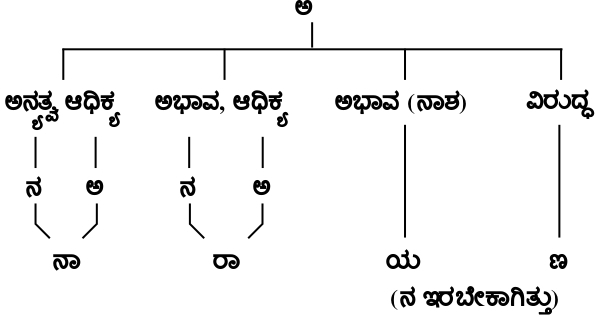
\includegraphics[scale=.4]{images/fig1.jpg}
\end{figure}

ಅನ್ಯತ್ವ= ಭಿನ್ನತೆ, ಆಧಿಕ್ಯ=ಮುಕ್ತಾಮುಕ್ತರಿಂದ ಆಧಿಕ್ಯ, ಅಭಾವ= ದೋಷಾಭಾವ,\break ವಿರುದ್ಧ=ಸರ್ವದೋಷವಿರುದ್ಧ ಗುಣಪೂರ್ಣತ್ವ.

\textbf{(೩೦)} ಅರಾಃ ಅನಿತ್ಯತ್ವವಿಕಾರಿತ್ವ ಪಾರತಂತ್ರ್ಯಾದಯೋ ದೋಷಾಃ-ಅರಾಃ ಎಂದರೆ ನಿತ್ಯತ್ವವಿಲ್ಲದಿರುವುದು (ನಾಶಹೊಂದುವಿಕೆ), ವಿಕಾರಿತ್ವ (ವಿಕಾರ ಹೊಂದುವಿಕೆ), ಪಾರತಂತ್ರ್ಯಾ\-ದಯಃ=ಸ್ವತಂತ್ರನಲ್ಲದೇ ಬೇರೆಯವರ ಅಧೀನದಲ್ಲಿರುವಿಕೆ ಇವೇ ಮೊದಲಾದ ದೋಷಗಳು. ತೇ ನ ವಿದ್ಯಂತೇ ಯಸ್ಯ ತತ್ ನಾರಂ-ಯಸ್ಯ=ಯಾರಿಗೆ, ತೇ=ಮೇಲೆ ಹೇಳಿದ ದೋಷಗಳು, ನ ವಿದ್ಯಂತೇ=ಇರುವುದಿಲ್ಲವೋ, ತತ್=ಅದು, ನಾರಂ= 'ನಾರಂ' ಎಂದು ಕರೆಸಿಕೊಳ್ಳಲಡುತ್ತದೆ. ಅಯನಮಿತಿ ಚ ಭಾವೇ ಲ್ಕುಟ್- ಅಯನಂ ಎಂಬ ಶಬ್ದಕ್ಕೆ ಲ್ಯುಟ್ ಪ್ರಯೋಗದಲ್ಲಿ ಭಾವೇ=ಇರುವಿಕೆ ಎಂಬರ್ಥದಲ್ಲಿ 'ಭಾವ' ಎಂಬರ್ಥವಾಗುತ್ತದೆ. ತಥಾ ಚ=ಆದುದರಿಂದ, ನಾರಂ ಅನಿತ್ಯತ್ವಾದಿದೋಷಶೂನ್ಯಂ ಅಯನಂ ಜ್ಞಾನಂ ಯಸ್ಯಾಸೌ ನಾರಾಯಣಃ-ಅನಿತ್ಯತ್ವಾದಿದೋಷಶೂನ್ಯಂ=ಅನಿತ್ಯತ್ವವೇ ಮೊದಲಾದ ದೋಷಗಳು ಇಲ್ಲದಿರುವ, ಅಯನಂ ಜ್ಞಾನಂ=ಜ್ಞಾನವು, ಯಸ್ಯ=ಯಾರಿಗೆ ಇದೆಯೋ, ಅಸೌ=ಅಂತಹವನು, ನಾರಾಯಣ (ಇಲ್ಲಿ ಅಯನಂ ಎಂದರೆ ಜ್ಞಾನವೆಂದರ್ಥ).

ಅನಿತ್ಯತ್ವ ವಿಕಾರಿತ್ವ ಮೊದಲಾದ ದೋಷರಹಿತವಾದ ಜ್ಞಾನ ಉಳ್ಳವನು ನಾರಾಯಣ (ನಾರಂ ಅಯನ).

ಯಥೋಕ್ತಂ- ಪ್ರಮಾಣಗಳಲ್ಲಿ ಹೀಗೆ ಹೇಳಲಾಗಿದೆ:-

ನಿತ್ಯಾನಂದೋ, ನಿತ್ಯಜ್ಞಾನೋ, ನಿತ್ಯಬಲಃ ಪರಮಾತ್ಮಾ-ಸರ್ವೋತ್ತಮನಾದ ಪರಬ್ರಹ್ಮನು, ನಿತ್ಯವಾದ (ನಾಶರಹಿತವಾದ) ಆನಂದವುಳ್ಳವನು, ನಿತ್ಯವಾದ (ತಿರೋಧಾನ ಹೊಂದದ) ಜ್ಞಾನಪೂರ್ಣನು, ನಿತ್ಯವಾದ (ಏಕಪ್ರಕಾರವಾದ) ಬಲವುಳ್ಳವನು.

\begin{center}
\textbf{ನಿತ್ಯವಾದ ಜ್ಞಾನವುಳ್ಳವನು ಎಂಬ ಕಾರಣದಿಂದ ನಾರಾಯಣ.}
\end{center}

\noindent
\textbf{ವಿಶೇಷಾಂಶ:\enginline{-}}

\begin{verse}
\textbf{ಸರ್ವೇ ನಿತ್ಯಾಃ ಶಾಶ್ವತಾಶ್ಚ ದೇಹಾಸ್ತಸ್ಯ ಪರಾತ್ಮನಃ~।}\\\textbf{ಪರಮಾನಂದ ಸಂದೋಹ ಜ್ಞಾನಮಾತ್ರಾಶ್ಚ ಸರ್ವಶಃ~।।}\\\textbf{ಸರ್ವೇ ಸರ್ವ ಗುಣಾತ್ಮಾನಃ ಸರ್ವಕರ್ತಾರ ಏವ ಚ~।।}
\end{verse}

\vauthor{(ಸತ್ತತ್ವರತ್ನಮಾಲಾ)}

ಪರಮಾತ್ಮನ (ಪರಬ್ರಹ್ಮನ) ಎಲ್ಲ ದೇಹಗಳೂ (ಮೂಲರೂಪ, ಅಸಂಖ್ಯಾತ ಅವತಾರರೂಪಗಳು) ನಿತ್ಯವಾದುವು, ವಿಕಾರವಿಲ್ಲದೇ ಸದಾ ಏಕ ಪ್ರಕಾರವಾಗಿರುವುವು; ಎಲ್ಲವೂ ನಿರ್ದೋಷವಾದ, ಜ್ಞಾನಾನಂದಮಯ ವಾಗಿರುವುವು; ಸರ್ವಸದ್ಗುಣಮೂರ್ತಿಗಳೇ, ಎಲ್ಲ ರೂಪಗಳೂ ಸೃಷ್ಟಾದಿ ಸಕಲ ಕಾರ್ಯಗಳನ್ನೂ ಮಾಡತಕ್ಕವುಗಳೇ,

\textbf{(೩೧)} ನಾರೇತ್ಯಸ್ಯ ಆವೃತ್ತಿಃ="ನಾರ" ಎಂದು ಎರಡು ಸಲ ಹೇಳತಕ್ಕದ್ದು. (i) ಅಯನಮಿತಿ ಚ ಭಾವೇ ಲ್ಯುಟ್=ಲ್ಯುಟ್ ಪ್ರಯೋಗದಲ್ಲಿ "ಅಯನಂ" ಶಬ್ದಕ್ಕೆ ಭಾವ (ಇರುವುದು) ಎಂದರ್ಥ. ತಥಾಚ=ಆದುದರಿಂದ, ನ ರೀಯತೆ=ನಾಶಹೊಂದುವುದಿಲ್ಲ (ವಿಕಾರ ಹೊಂದುವುದಿಲ್ಲ), ಇತಿ=ಹೀಗಿರುವುದರಿಂದ, ನರೋ ಭಗವಾನ್ ಹರಿಃ=ಷಡ್ಗುಣೈಶ್ಚರ್ಯಪೂರ್ಣನಾದ ಹರಿಗೆ "ನರ" ಎಂದು ಹೆಸರು. ತದಂಗಸ್ವೇದಜನಿತತ್ವೇನ=ಅವನ ("ನರ" ನ) ದೇಹದಿಂದ ಹುಟ್ಟಿದ ಬೆವರಿನ, ತತ್ಸಂಬಂಧಿನೀ=(ಬೆವರಿನ) ಸಂಬಂಧಉಳ್ಳದ್ದರಿಂದ, "ನಾರಾ" ವಿರಜಾನದೀ=ಎಂದರೆ ವಿರಜಾನದೀ (ವಿರಜಾನದಿಯಲ್ಲಿ ಹರಿಯುವುದು ಶ‍್ರೀಹರಿಯ ದೇಹದಿಂದ ಹುಟ್ಟಿದ ಬೆವರು ಎಂದು ತಾತ್ಪರ್ಯ), ತಸ್ಯಾಂ= ಅದರಲ್ಲಿ (ವಿರಜಾನದಿಯಲ್ಲಿ), ತತ್ಸ್ವಾನೇನ ಇತಿ ಯಾವತ್- ಸ್ನಾನಮಾಡುವುದರಿಂದ ಎಂಬ ಕಾರಣದಿಂದ;\break (ii) ನರಾಣಾಂ ಅಯಂ ನಾರಃ=ಚೇತನರ ಸಂಬಂಧ ಹೊಂದಿರುವುದಕ್ಕೆ "ನಾರ" ಎಂದು ಹೆಸರು. ಅಂದರೆ ಅನಾದಿಲಿಂಗ ಶರೀರರೂಪ ಪ್ರಕೃತಿಬಂಧಃ=ಚೇತನರ ಸ್ವರೂಪ ದೇಹದ ಮೇಲೆ ಅನಾದಿ ಕಾಲದಿಂದ ಲಿಂಗಶರೀರದ ರೂಪದಿಂದ ಇರುವ ಪ್ರಕೃತಿಬಂಧ (ಸತ್ತ್ವ\-ರಜಸ್ತಮೋ ಗುಣಗಳಿಂದ ಬಂಧಿಸಲ್ಪಟ್ಟಿರುವುದು). ತಸ್ಯ=ಈ ಅನಾದಿಪ್ರಕೃತಿಬಂಧನದ, ಅಯನಂ ಗಮನಂ=ನಾಶವು, ಯಸ್ಮಾತ್=ಯಾರಿಂದ ಆಗುತ್ತದೆಯೋ, ಅಸೌ=ಅಂತಹವನು, ನಾರಾಯಣ (ನಾರಂ ಅಯನಂ), ಜ್ಞಾನಿನಾಯಿತಿ ಯೋಗ್ಯತಯಾ ಸಂಬಂಧಃ (ಪ್ರಕೃತಿ ಬಂಧನಾಶವು), ಜ್ಞಾನಿನಾಂ=ಅಪರೋಕ್ಷ ಜ್ಞಾನ ಪಡೆದವರಿಗೆ, ಇತಿ= ಹೀಗೆಂದು, ಯೋಗ್ಯತಯಾ=ಯೋಗ್ಯವಾದ ರೀತಿಯಲ್ಲಿ, ಸಂಬಂಧಃ= ನಾಶದ ಸಂಬಂಧವನ್ನು (ತಿಳಿಯಬೇಕು) (ಪ್ರಕೃತಿ ಬಂಧನವು ಅಪರೋಕ್ಷ ಜ್ಞಾನಾನಂತರ ಪ್ರಾರಬ್ಧಕರ್ಮಭೋಗಿಸಿದ ನಂತರ ಲಿಂಗಶರೀರದ ನಾಶದೊಂದಿಗೆ ಆಗುತ್ತದೆ ಎಂದು ತಾತ್ಪರ್ಯ).

ಯಥೋಕ್ತಂ ವರಾಹಪುರಾಣೇ-ವರಾಹಪುರಾಣದಲ್ಲಿ ಹೀಗೆ ಹೇಳಲಾಗಿದೆ:-

\begin{verse}
\textbf{"ಪ್ರಧಾನಪರಮವ್ಯೋಮ್ನೋರಂತರಾ ವಿರಜಾನದೀ~।}\\\textbf{ಹರ್ಯಂಗಸ್ವೇದಜನಿತಾ ಗಂಗೈವಾಪರನಾಮಿಕಾ~।।}\\\textbf{ವಿಧೇರ್ದೇಹಾಪಗಮನೇ ಭಿನ್ನಲಿಂಗಶರೀರಕಾಃ~।}\\\textbf{ವಾಸುದೇವಂ ವಿಶಂತ್ಯೇತೇ ಪರಮಾನಂದರೂಪಿಣಮ್~।।"}
\end{verse}

ಪ್ರಧಾನಪರಮವ್ಯೋಮ್ನಃ=ಪ್ರಧಾನವೆಂದು ಹೇಳಲ್ಪಡುವ ಶ್ರೇಷ್ಠವಾದ ಅವ್ಯಾಕೃತಾಕಾಶದ, ಅಂತರಾ=ಒಳಗೆ, ಹರ್ಯಂಗಸ್ನೇದಜನಿತಾ=ಶ‍್ರೀಹರಿಯ ಶರೀರದ ಬೆವರಿನಿಂದ ಹುಟ್ಟಿದ, ಗಂಗಾ ಏವ ಅಪರನಾಮಿಕಾ=ಗಂಗೆಯೇ ಇನ್ನೊಂದು ಬೇರೆ ಹೆಸರಿನಿಂದ, ವಿರಜಾನದೀ=ವಿರಜಾನದೀ ಎಂದು ಪ್ರವಹಿಸುತ್ತದೆ. ವಿಧೇಃ=ಬ್ರಹ್ಮದೇವರ, ದೇಹಾಪಗಮನೇ=\-ಪ್ರಾಕೃತದೇಹವು ಬಿಟ್ಟುಹೋಗುತ್ತಿರಲು, ಭಿನ್ನಲಿಂಗ ಶರೀರಕಾಃ ತೇ=ಭಂಗಮಾಡಲ್ಪಟ್ಟ ಲಿಂಗಶರೀರ ಉಳ್ಳ ಈ ಚೇತನರು (ಲಿಂಗಶರೀರವನ್ನು ವಿರಜಾನದೀ ಸ್ನಾನದಿಂದ ಕಳೆದುಕೊಂಡ ಚೇತನರು), ಪರಮಾನಂದರೂಪಿಣಂ=ಶ್ರೇಷ್ಠವಾದ ಆನಂದಸ್ವರೂಪಿಯಾದ, ವಾಸುದೇವಂ=\-ವಾಸುದೇವ ನಾಮಕನಾದ ಶ‍್ರೀವಿಷ್ಣುವನ್ನು, ವಿಶಂತಿ=ಪ್ರವೇಶಿಸುತ್ತಾರೆ.

ಉಕ್ತಂ ಚ ಅನುವ್ಯಾಖ್ಯಾನೇ-ಅನುವ್ಯಾಖ್ಯಾನದಲ್ಲಿ ಈ ರೀತಿ ಹೇಳಲಾಗಿದೆ:- ಜ್ಞಾನಿನಾಂ ಮೋಕ್ಷದಶ್ಚ ಸಃ- ಜ್ಞಾನಿನಾಂ=ಅಪರೋಕ್ಷ ಜ್ಞಾನಯುಕ್ತರಾದವರಿಗೆ, ಮೋಕ್ಷದಃ ಚ=ಮೋಕ್ಷವನ್ನು ಕೊಡುವವನೂ ಸಹ, ಸ=ಅವನೇ (ಶ‍್ರೀವಿಷ್ಣುವೇ).

ವ್ಯಾಖ್ಯಾತಂ ಚೈವಂ ಸುಧಾಯಾಂ-ಈ ಪ್ರಮೇಯವು ಸುಧಾ ಗ್ರಂಥದಲ್ಲಿ ಈ ರೀತಿ ವ್ಯಾಖ್ಯಾನ ಮಾಡಲ್ಪಟ್ಟಿದೆ-"ಮೋಕ್ಷದಃ ಪ್ರಾಗುಕ್ತಬಂಧಾತ್" ಇತಿ-ಪ್ರಾಗುಕ್ತ ಬಂಧಾತ್=ಹಿಂದೆ ಹೇಳಿದ ಪ್ರಕೃತಿ ಬಂಧನದ ದೆಸೆಯಿಂದ (ಸಂಸಾರಾಖ್ಯ ಬಂಧನದಿಂದ), ಮೋಕ್ಷದಃ= ಮೋಕ್ಷವನ್ನು ಕೊಡುವವನು (ಬಿಡಿಸುವವನು), ಶ‍್ರೀಹರಿಯೇ.

\begin{center}
\textbf{ಅಪರೋಕ್ಷಜ್ಞಾನಿಗಳಿಗೆ ವಿರಜಾನದಿಸ್ನಾನದ ನಂತರ ಅನಾದಿ ಲಿಂಗಶರೀರರೂಪದಿಂದ ಇರುವ ಪ್ರಕೃತಿಬಂಧನವನ್ನು ನಾಶಮಾಡುವ ಕಾರಣದಿಂದ ನಾರಾಯಣ.}
\end{center}

\noindent
\textbf{ವಿಶೇಷಾಂಶ:\enginline{-}}

\begin{verse}
\textbf{ವಿಧೇರ್ದೇಹಾಪಗಮನೇ ಲಿಂಗಮಾತ್ರ ಶರೀರಿಣಃ~।}\\\textbf{ವಿರಾಜಾಯಾಂ ಕೃತಸ್ನಾನಾ ಬ್ರಹ್ಮಣಾ ಸಹ ಸರ್ವಶಃ~।}\\\textbf{ತ್ಯಕ್ತಲಿಂಗಾಃ ತತಃ ಸರ್ವೇ ಸ್ವರೂಪೇಣ ವ್ಯವಸ್ಥಿತಾಃ~।}\\\textbf{ವಿಶಂತಿ ವಾಸುದೇವಾಖ್ಯಂ ಹರೇ ರೂಪಂ ಚತುರ್ಥಕಂ~।।}
\end{verse}

\vauthor{-ವಿಷ್ಣು ರಹಸ್ಯ}

ಬ್ರಹ್ಮದೇವರ ಪ್ರಾಕೃತದೇಹವು ಬಿಟ್ಟುಹೋಗುತ್ತಿರಲು ಲಿಂಗಶರೀರ ಮಾತ್ರದಿಂದ ಇರುವವರು, ವಿರಜಾನದಿಯಲ್ಲಿ ಸ್ನಾನಮಾಡಿ, ಎಲ್ಲರೂ ಲಿಂಗಶರೀರಗಳನ್ನು ತ್ಯಜಿಸಿ ತಮ್ಮ ಸ್ವರೂಪ\-ದಿಂದ ಇರುತ್ತಾರೆ. ನಂತರ ಶ‍್ರೀಹರಿಯ ನಾಲ್ಕನೇ ರೂಪವಾದ (ಅನಿರುದ್ದ ಪ್ರದ್ಯುಮ್ನ ಸಂಕರ್ಷಣ, ವಾಸುದೇವ) ವಾಸುದೇವನೆಂಬ ರೂಪವನ್ನು ಬ್ರಹ್ಮದೇವರೊಡನೆ ಪ್ರವೇಶಿಸುತ್ತಾರೆ.

\begin{verse}
\textbf{ವಿರಜಾ ಚ ನದೀ ತತ್ರ ಗಂಗೈವಾಪರನಾಮಿಕಾ~।}\\\textbf{ಅಂತಿಮಾವರಣವ್ಯೋಮ್ನೋರಂತರೇ ವಿರಜಾನದೀ~।।}
\end{verse}

\vauthor{-ವಿಷ್ಣು ರಹಸ್ಯ}

ವೈಕುಂಠಲೋಕದಲ್ಲಿ ಗಂಗೆಯೇ (ವಿರಜಾ ಎಂಬ) ಮತ್ತೊಂದು ಹೆಸರಿನಿಂದ ಕರೆಯಲ್ಪಡು\-ತ್ತಾಳೆ. ಬ್ರಹ್ಮಾಂಡದ ಬಹಿರಾವರಣಗಳಲ್ಲಿ ಕಡೆಯದಾದ ಸತ್ವಗುಣಾವರಣ ಮತ್ತು ಅವ್ಯಾಕೃತಾಕಾಶಗಳ ಮಧ್ಯದಲ್ಲಿ ವಿರಜಾನದಿ ಪ್ರವಹಿಸುತ್ತದೆ.

\begin{verse}
\textbf{ವೈಕುಂಠಪರಿಘಾಕೃತ್ಯಾಂ ವಿರಜಾಯಾಂ ಸಮಸ್ತಶಃ~।}\\\textbf{ಮಹಾಲಕ್ಷ್ಮೀ ಸ್ವರೂಪಿಣ್ಯಾಂ ವಿಗಾಹ್ಯ ಪ್ರಕೃತೇಃ ಪರಂ~।।}\\\textbf{ಪ್ರಾರಬ್ಧಕರ್ಮಶೇಷಂ ಚ ಲಿಂಗದೇಹಾದಿಕಂ ತಥಾ~।}\\\textbf{ವಿನಾಶ್ಯ ಜಠರೇ ವಿಷ್ಣೋಃ ಪ್ರವಿಶ್ಯಾನುಗ್ರಹಾದ್ದರೇಃ~।।}
\end{verse}

\vauthor{-ಸತ್ತತ್ವರತ್ನಮಾಲಾ}

ಲಕ್ಷ್ಮೀಸ್ವರೂಪವಾದ ವೈಕುಂಠನಗರವನ್ನು ಸುತ್ತುವರಿದಿರುವ, ಮಹಾಲಕ್ಷ್ಮೀ ಸ್ವರೂಪವೇ ಆದ ವಿರಜಾನದಿಯಲ್ಲಿ ಸ್ನಾನಮಾಡಿ ಪ್ರಾರಬ್ಧಕರ್ಮಶೇಷವನ್ನೂ ಲಿಂಗದೇಹವನ್ನೂ ಕಳೆದುಕೊಂಡು ಶ‍್ರೀಹರಿಯ ಅನುಗ್ರಹದಿಂದ ವಿಷ್ಣುವಿನ ಉದರವನ್ನು ಪ್ರವೇಶಮಾಡಿ (ಸೃಷ್ಟಿಕಾಲ ಬಂದನಂತರ ಸ್ವಯೋಗ್ಯ ಆನಂದವನ್ನು ಅನುಭವಿಸುತ್ತಾರೆ).

\newpage

\begin{verse}
\textbf{ಅಜ್ಞಾನಾಂ ಜ್ಞಾನದೋ ವಿಷ್ಣುಃ ಜ್ಞಾನಿನಾಂ ಮೋಕ್ಷದಶ್ಚ ಸಃ~।}\\\textbf{ಆನಂದದಶ್ಚ ಮುಕ್ತಾನಾಂ ಸ ಏವೈಕೋ ಜನಾರ್ದನಃ~।।}
\end{verse}

\vauthor{-ಶ್ರುತಿ}

ಅಜ್ಞಾನಿಗಳಿಗೆ ಅಪರೋಕ್ಷ ಜ್ಞಾನವನ್ನು ಕೊಡುವವನೂ, ಅಪರೋಕ್ಷ ಜ್ಞಾನಿಗಳಿಗೆ ಮೋಕ್ಷವನ್ನು ದಯಪಾಲಿಸುವವನೂ, ಮೋಕ್ಷದಲ್ಲಿ ಮುಕ್ತರಿಗೆ ಆನಂದವನ್ನು ದೊರಕಿಸುವವನೂ ಆ ಜನಾರ್ದನ ಎಂಬ ನಾಮದ ಶ‍್ರೀಹರಿಯೇ, ಅನ್ಯರಲ್ಲ,

\begin{verse}
\textbf{ಬಂಧಕೋ ಭವಪಾಶೇನ ಮೋಚಕಶ್ಚ ಸ ಏವ ಹಿ~।}
\end{verse}

\vauthor{-ಶ್ರುತಿ.}

ಸಂಸಾರಪಾಶದಿಂದ ಬಂಧಿಸುವವನೂ, ಆ ಪಾಶದಿಂದ ಬಿಡುಗಡೆ ಮಾಡುವವನೂ ಆ ಶ‍್ರೀಹರಿಯೇ.

\textbf{(೩೨)} ನರಶಬ್ದೋ ಜ್ಞಾನಿಮಾತ್ರಪರಃ -"ನರ" ಶಬ್ದವು ಜ್ಞಾನಿಗಳನ್ನು ಉದ್ದೇಶಿಸಿ ಹೇಳು\-ವಂತಹುದು. ಲ್ಯುಟ್ ಚ ಭಾವೇ-ಭಾವ (ಇರುವುದು) ಎಂಬರ್ಥದಲ್ಲಿ ಲ್ಯುಟ್ ಪ್ರಯೋಗ ಬರುತ್ತದೆ. ತಥಾ ಚ=ಹೀಗಿರುವುದರಿಂದ, ನರಾಣಾಂ ಇದಂ ನಾರಂ ಚೇತಃ-"ನರ"ರ (ಜ್ಞಾನಿಗಳ) ಸಂಬಂಧ ಹೊಂದಿರುವುದು, ನಾರಂ ಚೇತಃ=ಹೃದಯ, ತತ್ಪ್ರತಿ ತದ್ವಿಷಯ ಭಾವನಾಯೇತಿಯಾವತ್-ನಾರಂ (ಹೃದಯ) ಕುರಿತು, ಅಂದರೆ ಹೃದಯದಲ್ಲಿ ದರ್ಶನಕೊಡುವುದೂ ಬಿಡುವುದೂ ಎಂಬ ಕಾರಣದಿಂದ, ಅಯನಂಗಮನಾಗಮನಂ ಯಸ್ಯಾಸೌ\break ನಾರಾಯಣಃ- ಯಸ್ಯ=ಯಾರಿಗೆ, ಅಯನಂ=ಗಮನಾಗಮನಂ=ಹೋಗುವುದು, ಹಿಂದಿರು\-ಗುವುದು (ಸಾಧ್ಯವೋ), ಅಸೌ=ಅಂತಹವನು, ನಾರಾಯಣ (ಜ್ಞಾನಿಗಳ ಹೃದಯದಲ್ಲಿ ಕಾಣಿಸಿ\-ಕೊಳ್ಳುವುದು, ಅದೃಶ್ಯನಾಗುವುದು ಎಂದು ತಾತ್ಪರ್ಯ, ಜ್ಞಾನಿಗಳೆಂದರೆ ಅಪರೋಕ್ಷ\-ಜ್ಞಾನಿಗಳೆಂಬುದು ಸ್ಪಷ್ಟ).

\textbf{ಯಥೋಕಂ, ಭಾಗವತೇ ನಾರದೇನ}-ನಾರದರಿಂದ ಹೇಳಲ್ಪಟ್ಟ ವಿಷಯ ಭಾಗವತದಲ್ಲಿ ಹೀಗೆ ನಿರೂಪಿಸಲಾಗಿದೆ-\textbf{"ಆಹೂತ ಇವ ಮೇ ಶೀಘ್ರಂ ದರ್ಶನಂ ಯಾತಿ ಚೇತಸಿ"}\break -ಕರೆಸಿಕೊಂಡವನಂತೆ ನನ್ನ ಹೃದಯದಲ್ಲಿ ಶೀಘ್ರವಾಗಿ ದರ್ಶನವನ್ನು ಕೊಡುತ್ತಾನೆ.

ಪರಮಾತ್ಮನು ತನ್ನ ಇಚ್ಛಾನುಸಾರ ಅಪರೋಕ್ಷಜ್ಞಾನಿಗಳ ಹೃದಯಲ್ಲಿ ದರ್ಶನಕೊಡುತ್ತಾನೆ ಹಾಗೂ ಅದೃಶ್ಯನಾಗುತ್ತಾನೆಂದು ತಾತ್ಪರ್ಯ.

\begin{center}
\textbf{ಅಪರೋಕ್ಷ ಜ್ಞಾನಿಗಳ ಅಂತಃಕರಣಕ್ಕೆ ವಿಷಯನಾಗಿರುವ ಕಾರಣದಿಂದ ನಾರಾಯಣ.}
\end{center}

\textbf{(೩೩)} ಪೂರ್ವವನ್ನರಶಬ್ದೋ ಜ್ಞಾನಿಪರಃ-ಹಿಂದೆ ಹೇಳಿದಂತೆ "ನರ" ಶಬ್ದವು ಜ್ಞಾನಿಗಳನ್ನು ಕುರಿತು ಹೇಳುವುದಾಗಿದೆ. ಲ್ಯುಟ್ ಚ ಭಾವೇ=ಭಾವಾರ್ಥದಲ್ಲಿ (ಸಂಬಂಧ ಎಂದು ಹೇಳುವಾಗ) ಲ್ಯುಟ್ ಪ್ರಯೋಗ ಬರುತ್ತದೆ. ತಥಾ ಚ=ಹಾಗೆಯೇ, ನರಾಣಾಂ ಜ್ಞಾನಿನಾಂ= ಜ್ಞಾನಿಗಳ, ಸಮೂಹಃ=ಗುಂಪು, ನಾರಶಬ್ದೇನೋಚ್ಯತೇ="ನಾರ" ಎಂಬ ಶಬ್ದದಿಂದ ಹೇಳಲ್ಪಡುತದೆ. ಏವಂ ಚ=ಆದುದರಿಂದ, ನರಾನ್= ಜ್ಞಾನಿಸಂಘಾನ್=ಜ್ಞಾನಿಗಳ ಸಮುದಾಯವನ್ನು ಉದ್ದಿಶ್ಯ ಸ್ವಾಂಫ್ರಿರೇಣುಭಿರ್ವಾತನೀತೈಃ ಅಗ್ರೇಸರಾನ್ ತಾನ್ ಶೋಧ\-ಯಾಮಿ ಇತ್ಯಾಶಯೇನ ಇತಿ ಯಾವತ್‌-ಉದ್ದಿಶ್ಯ=ಲಕ್ಷ್ಮದಲ್ಲಿಟ್ಟು, ಸ್ವಾಂಫ್ರಿರೇಣುಭಿಃವಾತನೀತೈಃ=ಗಾಳಿಯಿಂದ ತರಲ್ಪಟ್ಟ ತನ್ನ ಪಾದದ ಧೂಳಿನಿಂದ, ತಾನ್ ಅಗ್ರೇಸರಾನ್=ಮುಂದೆ ಹೋಗುತ್ತಿರುವವರನ್ನು ಶೋಧಯಾಮಿ=(ನಿರ್ದೋಷರಾಗುವರಂತೆ) ಸ್ವಚ್ಛಮಾಡುತ್ತೇನೆ,\break ಇತ್ಯಾಶಯೇನ ಇತಿ ಯಾವತ್=ಹೀಗೆಂಬ ಅಭಿಪ್ರಾಯದಿಂದ ಎಂಬಂತೆ; ಅಯನಂ ತದೀಯಪಶ್ಚಾದ್ಘಾಗೇ ಗಮನಂ ಯಸ್ಯಾಸೌ ನಾರಾಯಣಃ-ಅಯನಂ=ತದೀಯ ಪಶ್ಚಾದ್ಭಾಗೇ ಗಮನಂ= ನಂತರ (ಸ್ವಚ್ಛಮಾಡಲು) ಅವರ ಹಿಂದುಗಡೆ ಹೋಗುವುದು, ಯಸ್ಯ= ಯಾರಿಗೋ, ಅಸೌ=ಅಂತಹವನು, ನಾರಾಯಣ (ನಾರಂ ಅಯನಂ).

(ಜ್ಞಾನಿಗಳನ್ನು ತನ್ನ ಪಾದರಜಸ್ಸಿನಿಂದ ಪಾಪರಹಿತರನ್ನಾಗಿ ಮಾಡಲು ಅವರ ಹಿಂದೆ\break ಹೋಗುವವನು-ಅಯನಂ ಅಂದರೆ ಅವನಿಗೆ ಯೋಗ್ಯವಾದ ಗತಿಯನ್ನು ಕೊಡುವವನು).

ಯಥೋಕ್ತಂ ಭಾಗವತೇ-ಭಾಗವತದಲ್ಲಿ ಹೇಳಿದಂತೆ-

\begin{verse}
\textbf{ನಿರಪೇಕ್ಷಂ ಮುನಿಂ ಶಾಂತಂ ನಿರ್ವೈರಂ ಸಮದರ್ಶಿನಂ~।}\\\textbf{ಅನುವ್ರಜಾಮ್ಯಹಂ ನಿತ್ಯಂ ಪೂಯೇಯೇತ್ಯಂಫ್ರಿರೇಣುಭಿಃ~।।}
\end{verse}

ನಿರಪೇಕ್ಷಂ= ಐಹಿಕ ಫಲದಲ್ಲಿ ಅಪೇಕ್ಷೆ ಇಲ್ಲದ, ಶಾಂತಂ=ಶಾಂತ ಸ್ವಭಾವದಿಂದ ಕೂಡಿದ, ನಿರ್ವೈರಂ=ಯಾರಲ್ಲಿಯೂ ದ್ವೇಷಮಾಡದ, ಸಮದರ್ಶಿನಂ=ನಿರ್ದೋಷನಾದ ಪರಮಾತ್ಮ\-ನನ್ನು ನೋಡುವ, ಮುನಿಂ= ಮನನಶೀಲರಾದ, (ಜ್ಞಾನಿಗಳನ್ನು) ನಿತ್ಯಂ=ಯಾವಾಗಲೂ, ಅಂಫ್ರಿ ರೇಣುಭಿಃ=ನನ್ನ ಪಾದದ ಧೂಳಿನಿಂದ, ಪೂಯೇಯ ಇತಿ= ಪವಿತ್ರರನ್ನಾಗಿ ಮಾಡಲು, ಅಹಂ=ನಾನು, ಅನುವ್ರಜಾಮಿ=ಅನುಸರಿಸಿ ಹೋಗುತ್ತೇನೆ.

ವ್ಯಾಖ್ಯಾತಂ ಭಗವತ್ಪಾದೈಃ-ಶ‍್ರೀಮದಾಚಾರ್ಯರಿಂದ ಹೀಗೆ ವ್ಯಾಖ್ಯಾನ ಮಾಡಲ್ಪ\-ಟ್ಟಿದೆ-

\begin{verse}
\textbf{ಸ್ವಾಂಘ್ರಿರೇಣುಭಿಃ ತಂ ಶೋಧಯಾಮಿ ಇತ್ಯುನುವ್ರಜಾಮಿ~।}\\\textbf{ಅಗ್ರತೋ ಗಮನೇ ವಿಷ್ಣೋಃ ಪಾದಸ್ಪೃಷ್ಟರಜೋ ಭವೇತ್~।।}\\\textbf{ತಸ್ಯಾಂಫ್ರಿರೇಣುಭಿರ್ವಾತನೀತ್ಸೆಃ ಅಗ್ರೇಸರಃ ಶುಚಿಃ~।}\\\textbf{ಅತಃ ಸ್ವಭಾಕ್ತಂ ಪೂಯೇಯೇತ್ಪನುವ್ರಜತಿ ಕೇಶವಃ~।।}
\end{verse}

ತಂ=ಅವನನ್ನು (ಭಕ್ತನನ್ನು), ಸ್ವಾಂಘ್ರಿರೇಣುಭಿಃ=ತನ್ನ ಪಾದದ ಧೂಳಿನ ಕಣಗಳಿಂದ, ಶೋಧಯಾಮಿ=ಶುದ್ಧನನ್ನಾಗಿ ಮಾಡುತ್ತೇನೆ. ಇತಿ=ಈ ಉದ್ದೇಶದಿಂದ, ಅನು\-ವ್ರಜಾಮಿ=\break ಅನುಸರಿಸಿ ಹೋಗುತ್ತೇನೆ. (ಭಕ್ತನು) ಅಗ್ರತಃ=ಮುಂದೆ, ಗಮನೇ (ಸತಿ)=ಹೋಗುತ್ತಿರಲು, ವಿಷ್ಣೋ=ವಿಷ್ಣುವಿನ, ಪಾದಸ್ಸಷ್ಟರಜಃ-ಪಾದಕ್ಕೆ ಸ್ಪರ್ಶವಾದ ಧೂಳು, ಭವೇತ್=ಹುಟ್ಟುತ್ತದೆ, ವಾತನೀತೈಃ=ಗಾಳಿಯಿಂದ ತರಲ್ಪಟ್ಟ, ತಸ್ಯಾಂಫ್ರಿ ರೇಣುಭಿಃ=ಅವನ ಪಾದದ ಧೂಳಿನ ಕಣಗಳಿಂದ, ಅಗ್ರೇಸರಃ=ಮುಂದೆ ಹೋಗುತ್ತಿರುವ ಭಕ್ತನು, ಶುಚಿಃ ಭವೇತ್=ಶುದ್ದನಾಗಿ ಆಗುವನು, ಅತಃ=ಆ ಕಾರಣದಿಂದ ಸ್ವಭಕ್ತಂ=ತನ್ನ ಭಕ್ತನನ್ನು, ಪೂಯೇಯ ಇತಿ=ಪವಿತ್ರನನ್ನಾಗಿ ಮಾಡಲು, ಕೇಶವಃ=ಶ‍್ರೀಹರಿಯು, ಅನುವ್ರಜತಿ=ಭಕ್ತರನ್ನು ಅನುಸರಿಸಿ ಹೋಗುತ್ತಾನೆ.

\textbf{ತಾತ್ಪರ್ಯ:} ಪರಮಾತ್ಮನ ಪಾದಧೂಳು ಶರೀರಕ್ಕೆ ಸ್ವರ್ಶವಾದರೆ ಭಕ್ತನು ಪವಿತ್ರನಾಗುತ್ತಾನೆ. ಭಕ್ತನು ಮುಂದೆ ಪ್ರಯಾಣಮಾಡುತ್ತಿರುವಾಗ, ಪರಮಾತ್ಮನು ಅವನನ್ನು ಹಿಂಬಾಲಿಸುತ್ತಾನೆ. ಪರಮಾತ್ಮನ ಪಾದಸ್ಪರ್ಶವಾದ ಧೂಳು ಗಾಳಿಬೀಸುವುದರಿಂದ ತರಲ್ಪಟ್ಟು ಮುಂದೆ ಹೋಗುತ್ತಿರುವ ಭಕ್ತನ ಮೇಲೆ ಬೀಳುತ್ತದೆ. ಈ ಕಾರಣದಿಂದ ಭಗವಂತನು ತನ್ನ ಭಕ್ತರನ್ನು ಅನುಸರಿಸಿ ಹೋಗುತ್ತಾನೆ.

\begin{center}
\textbf{ಮುಂದೆ ಹೋಗುತ್ತಿರುವ ಜ್ಞಾನಿಗಳಿಗೆ ಗಾಳಿಯಿಂದ ತರಲ್ಪಟ್ಟ ತನ್ನ ಪಾದದ ಧೂಳಿನಿಂದ ಪವಿತ್ರರನ್ನಾಗಿ ಮಾಡುವ ಅಭಿಪ್ರಾಯದಿಂದ ಜ್ಞಾನಿಗಳ ಹಿಂದೆ ಹೋಗುವ ಕಾರಣದಿಂದ ನಾರಾಯಣ}
\end{center}

\textbf{(೩೪)} ಉಕ್ತರೀತ್ಯಾ ನರಃ ಚತುರ್ಮುಖಃ-ಮೇಲೆ ಹೇಳಿದಂತೆ ಚತುರ್ಮುಖ ಬ್ರಹ್ಮದೇವರಿಗೆ "ನರ'' ಎಂದು ಹೇಳಲಾಗುತ್ತದೆ. ಲ್ಯುಟ್ ಚ ಭಾವೇ=ಭಾವಾರ್ಥದಲ್ಲಿ ಲ್ಯುಟ್ ಪ್ರಯೋಗ ಬರಲಾಗಿ, ತಸ್ಯೇದಂ ಶರೀರಂ ನಾರಂ=ಬ್ರಹ್ಮನ ಶರೀರಕ್ಕೆ ಸಂಬಂಧಿಸಿದುದು "ನಾರಂ'' ಎಂದಾಗುತ್ತದೆ. ಪದಾಗ್ರಪರಪರ್ಯಾಯ ಪ್ರಪದೋಪಲಕ್ಷಣಮೇತತ್-ಇಲ್ಲಿರುವ ಅರ್ಥ ವಿವರಣೆಯಲ್ಲಿ ಪದಾಗ್ರ (ಪಾದದ ಮುಂದಿನ ಭಾಗ) ಅಪರ ಪರ್ಯಾಯ ಪ್ರಪದ=ಪದಾಗ್ರ ಪದಕ್ಕೆ ಸಮಾನಾರ್ಥವುಳ್ಳ "ಪ್ರಪದ' ಎಂಬ ಪದದಿಂದ ಉಪಲಕ್ಷಿತವಾಗಿದೆ.

("ಪದಾಗ್ರ" ಮತ್ತು "ಪ್ರಪದ" ಎಂಬ ಪದಗಳು ಒಂದೇ ಅರ್ಥ ಉಳ್ಳವುಗಳು, ಅಂದರೆ ಪಾದದ ಮುಂಭಾಗ ಎಂದರ್ಥ. ಬ್ರಹ್ಮದೇವರ "ಶರೀರವನ್ನು" ಎಂದು ಹೇಳುವ ಬದಲಾಗಿ ಬ್ರಹ್ಮದೇವರ "ಪಾದದ ಮುಂಭಾಗ" ಎಂದು ಉಪಲಕ್ಷಣದಿಂದ ಹೇಳಲಾಗಿದೆ. ಪಾದದ ಮುಂಭಾಗವೆಂದರೆ ಇಡೀ ಶರೀರವೇ ಎಂದರ್ಥ).

ತದ್ವಾರಾ ಅಯನಂ ಗಮನಂ ಚತುರ್ಮುಖಶರೀರೇ ಯಸ್ಯಾಸೌ ವಾಸುದೇವೋ ನಾರಾಯಣಃ ಯಸ್ಯ=ಯಾರಿಗೆ, ತದ್ವಾರಾ=ಪಾದದ ಮುಂದಿನ ಭಾಗದಿಂದ, ಚತುರ್ಮುಖಶರೀರೇ=ಬ್ರಹ್ಮನ ಶರೀರದಲ್ಲಿ, ಅಯನಂ ಗಮನಂ=ಪ್ರವೇಶವು (ಆಗುತ್ತದೆಯೋ), ಅಸೌ-ಅಂತಹವನು, ವಾಸುದೇವಃ=ವಾಸುದೇವನೆಂದು ಕರೆಯಲ್ಪಡುವ ನಾರಾಯಣ (ನಾರಂ ಅಯನಂ).

ಯಥೋಕ್ತಂ- "ತಂ ಪ್ರಪದಾಭ್ಯಾಂ ಪ್ರಾಪದ್ಯತ ಬ್ರಹೇಮಂ ಪುರುಷಂ" ಬ್ರಹ್ಮ=\-ಪರಬ್ರಹ್ಮನು (ನಾರಾಯಣನು), ಇಮಂ ಪುರುಷಂ=ಈ ಚತುರ್ಮುಖನನ್ನು, ಪ್ರಪದಾಭ್ಯಾಂ= ಅವನ ಎರಡು ಪಾದಗಳ ಮುಂಭಾಗದ ಮೂಲಕ, ಪ್ರಾಪದ್ಯತ=ಹೊಂದಿದನು (ಪ್ರವೇಶಿಸಿದನು) ಹೀಗೆ ಪ್ರಮಾಣದಲ್ಲಿ ಹೇಳಲಾಗಿದೆ.

ಉಕಂ ಚ ಐತರೇಯಭಾಷ್ಯೇ-ಐತರೇಯ ಭಾಷ್ಯದಲ್ಲಿಯೂ ಹೇಳಲಾಗಿದೆ:-

\begin{verse}
\textbf{ತಮಿಮಂ ಪ್ರಥಮಜ್ಞಾನೀ ಪುರುಷಂ ಚತುರಾನನಂ~।}\\\textbf{ವಾಸುದೇವಾಭಿದಂ ಬ್ರಹ್ಮ ಪ್ರಾಪ ಪ್ರಪದಯೋಃ ಪುರಾ~।।}
\end{verse}

ಪ್ರಥಮಜ್ಞಾನೀ=ಜ್ಞಾನೋತ್ಪಾದಕನಾದ, ವಾಸುದೇವಾಭಿದಂ ಬ್ರಹ್ಮ= ವಾಸುದೇವನೆಂದು ಹೇಳಲ್ಪಡುವ ಪರಬ್ರಹ್ಮನು, ಇಮಂ ಚತುರಾನನಂ ಪುರುಷಂ= ಈ ಚತುರ್ಮುಖನ ಶರೀರವನ್ನು, ಪುರಾ=ಹಿಂದೆ, ಪ್ರಪದಯೋಃ =ಪಾದಗಳ ಮುಂಭಾಗದಿಂದ, ಪ್ರಾಪ=ಹೊಂದಿದನು (ಪ್ರವೇಶಿಸಿದನು).

\begin{center}
\textbf{ಪಾದದ ಮುಂದಿನ ಭಾಗದ ಮೂಲಕ ಚತುರ್ಮುಖಬ್ರಹ್ಮದೇವರ ಶರೀರದಲ್ಲಿ ಪ್ರವೇಶಮಾಡಿದ ಕಾರಣದಿಂದ ನಾರಾಯಣ.}
\end{center}

\textbf{(೩೫)} ನ ವಿದ್ಯತೇ ರಂ ರಮಣಂ ಯೇಷಾಂ ತೇ- ಯೇಷಾಂ= ಯಾರಿಗೆ, ರಂ ರಮಣಂ=ಸುಖದಿಂದ ಕ್ರೀಡೆಯು, ನ ವಿದ್ಯತೇ= ಇರುವುದಿಲ್ಲವೋ, ತೇ=ಅಂತಹವರು, ಇತಿ=ಹೀಗೆಂಬ, ವ್ಯುತ್ಪತ್ತ್ಯಾ= ಪದರಚನೆಯಿಂದ, ನರ ಶಬ್ದೋ="ನರ" ಎಂಬ ಶಬ್ದವು,\break ದೋಷಿಜನಪರ=ದೋಷದಿಂದ ಕೂಡಿದ (ಪಾಪಿಗಳ) ಜನರನ್ನು ಕುರಿತು ಹೇಳುವಂತಹುದು; ತಥಾ ಚ=ಆದುದರಿಂದ, ನರಾನಾಂ ದೋಷಜನಾನಾಂ ಇದಂ ನಾರಂ= ದೋಷಯುಕ್ತ ಜನಗಳಿಗೆ ಸಂಬಂಧಿಸಿದುದು "ನಾರಂ" ಎಂದಾಗುತ್ತದೆ. ತದೀಯಂ ಚಿತ್ತಮಿತಿ ಯಾವತ್=ಅವರ ಸಂಬಂಧವೆಂದರೆ ಅವರ ಮನಸ್ಸು ಎಂದರ್ಥ. ತಸ್ಮಾತ್ ಅಯನಂ ಗಮನಂ ಯಸ್ಯಾಸೌ ನಾರಾಯಣಃ- ಯಸ್ಯ=ಯಾರಿಗೆ, ತಸ್ಮಾತ್=ದೋಷಯುಕ್ತ ಜನರ ಮನಸ್ಸಿನ ದೆಸೆಯಿಂದ, ಅಯನಂ ಗಮನಂ=ಹೊರಗೆ ಹೋಗುವಿಕೆಯು (ಇರುತ್ತದೆಯೋ), ಅಸೌ=ಅಂತಹವನು ನಾರಾಯಣ (ನಾರಂ ಅಯನಂ).

ದೋಷಿಣಾಂ ಚಿತ್ತವಿಷಯೋ ನ ಭವತೀತ್ಯರ್ಥಃ-ದೋಷಿಣಾಂ= ದೋಷಯುಕ್ತರಾದ ಜನರ, ಚಿತ್ತವಿಷಯ=ಮನಸ್ಸಿಗೆ ವಿಷಯನಾಗಿ (ಅಂದರೆ ಧ್ಯಾನಮಾಡಲ್ಪಡುವವನಾಗಿ), ನ ಭವತಿ ಇತಿ ಅರ್ಥಃ= ಆಗುವುದಿಲ್ಲವೆಂದರ್ಥ (ಪಾಪಯುಕ್ತರಾದ ಜನರ ಮನಸ್ಸಿಗೆ ಪರಮಾತ್ಮನು ಧ್ಯಾನವಿಷಯನಾಗುವುದಿಲ್ಲ. ಪಾಪಿಗಳು ಅವನನ್ನು ಧ್ಯಾನ ಮಾಡುವುದಿಲ್ಲವೆಂದು ತಾತ್ಪರ್ಯ. ಪರಮಾತ್ಮನು ಪಾಪಿಗಳ ಹೃದಯದಲ್ಲಿ ಇರುವುದೇ ಇಲ್ಲ ಎಂಬರ್ಥವಲ್ಲ. ಹೀಗೆ ಅರ್ಥಮಾಡಿದರೆ ಅವನ ವ್ಯಾಪ್ತತ್ವಕ್ಕೆ ಹಾನಿ ಬರುತ್ತದೆ. ಹೃದಯದಲ್ಲಿದ್ದರೂ ಧ್ಯಾನಕ್ಕೆ ವಿಷಯನಾಗುವುದಿಲ್ಲವೆಂದೇ ತಿಳಿಯಬೇಕು).

\newpage

ಯಥೋಕ್ತಂ ಭಾಗವತೇ-ಭಾಗವತದಲ್ಲಿ ಹೀಗೆ ಹೇಳಲಾಗಿದೆ-

\begin{verse}
\textbf{ಸಮೀಪಸ್ಥೋಽಪಿ ದೂರಸ್ಥೋ ಭಗವಾನ್ ದುಷ್ಟಚೇತಸಾಮ್~।}
\end{verse}

ದುಷ್ಟಚೇತಸಾಂ=ಪಾಪಿಗಳಿಗೆ (ವಿಷ್ಣುದ್ವೇಷಿಗಳಿಗೆ), ಭಗವಾನ್= ಷಡ್ಗುಣೈಶ್ಚರ್ಯಪೂರ್ಣನಾದ ಶ‍್ರೀಹರಿಯು, ಸಮೀಪಸ್ಥಃ ಅಪಿ=ಹತ್ತಿರದಲ್ಲಿಯೇ ಇದ್ದರೂ ಸಹ, ದೂರಸ್ಥಃ=(ಅವರ ಮನಸ್ಸಿನಿಂದ) ದೂರದಲ್ಲಿಯೇ ಇರುವನು. (ಸಮೀಪದಲ್ಲಿಯೇ ಪರಮಾತ್ಮನು ಇದ್ದರೂ ಸಹ ಅರಿಯದೆ ಪಾಪಾತ್ಮರು ಅವನನ್ನು ಧ್ಯಾನಿಸುವುದಿಲ್ಲ).

\begin{center}
\textbf{ಪಾಪಿಷ್ಠರ ಅಂತಃಕರಣಕ್ಕೆ ವಿಷಯನಾಗುವುದಿಲ್ಲವೆಂಬ ಕಾರಣದಿಂದ ನಾರಾಯಣ.}
\end{center}

\noindent
\textbf{ವಿಶೇಷಾಂಶ:\enginline{-}}

\begin{verse}
\textbf{ನ ಹೈಪುಣ್ಯವತಾಂ ಲೋಕೇ ಮೂಢಾನಾಂ ಕುಟಿಲಾತ್ಮನಾಂ~।}\\\textbf{ಭಕ್ತಿರ್ಭವತಿ ಗೋವಿಂದೇ ಸ್ಮರಣಂ ಕೀರ್ತನಂ ತಥಾ~।।}
\end{verse}

\vauthor{(ಕೃಷ್ಣಾಮೃತಮಹಾರ್ಣವ)}

ಮೂರ್ಖರಿಗೂ, ಮಿಥ್ಯಾಜ್ಞಾನಿಗಳಿಗೂ, ಪುಣ್ಯರಹಿತರಿಗೂ, ಗೋವಿಂದನಲ್ಲಿಯೂ ಅವನ ಸ್ಮರಣೆ ಗುಣಕೀರ್ತನೆಗಳಲ್ಲಿಯೂ ಆಸಕ್ತಿ ಹುಟ್ಟುವುದಿಲ್ಲ, ಭಕ್ತಿ ಆಸಕ್ತಿ ಇಲ್ಲದ ಮೇಲೆ ಅವನ ದರ್ಶನ ಸಾಧ್ಯವೇ? ಇಲ್ಲವೇ ಇಲ್ಲ.

\begin{verse}
\textbf{ಭಕ್ತ್ಯಾ ತ್ವನನ್ಯಯಾ ಶಕ್ಯ ಅಹಮೇವಂ ವಿಧೋಽರ್ಜುನ~।}\\\textbf{ಜ್ಞಾತುಂ ದ್ರಷ್ಟುಂ ಚ ತತ್ವೇನ ಪ್ರವೇಷ್ಟುಂ ಚ ಪರಂತಪ~।।}
\end{verse}

\vauthor{(ಗೀತಾ)}

ಅರ್ಜುನನೇ, ನಾನು ಹೇಗಿರುವೆನೋ ಆ ರೀತಿಯಲ್ಲಿ ತಿಳಿಯಲು, ನೋಡಲು, ನನ್ನಲ್ಲಿ ಪ್ರವೇಶಿಸಲು ಅಸಾಧಾರಣವಾದ ಭಕ್ತಿಯಿಂದಲೇ ಶಕ್ಯನು. ಅನ್ಯಥಾ ಇಲ್ಲ,

\begin{verse}
\textbf{ದೂರಾದ್ದೂರತರಂ ಯತ್ತು ತದೇವಾಂತಿಕಮಂತಿಕಾತ್~।}\\\textbf{ಆನಂದಸ್ಯ ಪದಂ ವಂದೇ ಬ್ರಹೇಂದ್ರಾದ್ಯಭಿವಂದಿತಮ್~।।}
\end{verse}

\vauthor{(ದ್ವಾದಶಸ್ತೋತ್ರ)}

ಆನಂದಶಬ್ದವಾಚ್ಯನಾದ ಶ‍್ರೀಹರಿಯ ಪಾದವು ಭಕ್ತಿರಹಿತನಾಗಿರುವವನಿಗೆ ಅತ್ಯಂತದೂರ; ಆದರೆ ಭಕ್ತನಿಗೆ ಅತ್ಯಂತ ಸಮೀಪ. ಬ್ರಹ್ಮಾದಿಗಳಿಂದ ವಂದಿತವಾದ ಅಂತಹ ಶ‍್ರೀಹರಿಯ ಪಾದವನ್ನು ನಮಸ್ಕರಿಸುತ್ತೇನೆ.

\textbf{(೩೬)} ನ ವಿದ್ಯತೇ ರಂ ರಮಣಂ ಯೇಷಾಂ ತೇ ನರಾಃ-ಯೇಷಾಂ=ಯಾರಿಗೆ, ರಂ=ರಮಣಂ=ಕ್ರೀಡಿಸುವ ಸುಖವು, ನ ವಿದ್ಯತೇ-ಇಲ್ಲವೋ, ತೇ=ಅವರು, ನರಾಃ="ನರಾ?" ಎಂದು ಕರೆಯಲ್ಪಡುವರು. ತೇಷಾಂ ಸಂಬಂಧಿ=ಅವರ ಸಂಬಂಧ ಉಳ್ಳದ್ದು ನರಕಾದಿ ಸ್ಥಾನಂ ನಾರಂ=ನರಕವೇ ಮುಂತಾದ (ದುಃಖಪೂರಿತವಾದ) ಪ್ರದೇಶವು, ನಾರಂ ಎಂದು ಹೇಳಲ್ಪಡುತ್ತದೆ. "ನ ಚ ರಮಂತ್ಯಹೋ ಅಸದುಪಾಸನಯಾಽತ್ಮಹಾನಃ"-ಇತಿ ಶ್ರುತಿಗೀತಾವಚನಾತ್, ಅಸದುಪಾಸನಯಾ=ಮಿಥ್ಯಾ ಜ್ಞಾನದಿಂದ ಉಪಾಸನೆ ಮಾಡುವ, ಆತ್ಮಹನಃ=ತಮ್ಮ ಸ್ವರೂಪವನ್ನೇ ನಾಶಮಾಡಕೊಳ್ಳುವ ಜನರು, ನ ಚ ರಮಯಂತಿ=(ಸ್ವರ್ಗಾದಿ) ಸುಖವನ್ನು ಹೊಂದುವುದೇ ಇಲ್ಲ, ಅಹೋ=ಆಶ್ಚರ್ಯ-ಹೀಗೆಂದು ಶ್ರುತಿಗೀತೆಯಲ್ಲಿ ಹೇಳಲಾಗಿದೆ.

ತದೇವ ಅಯನಂ ತತ್ರತ್ಯಜನಪ್ರೇರಣಾಯ ಅವಾಸಸ್ಥಾನಂ ಯಸ್ಯಾಽಸೌ ಭಗವಾನ್ ನಾರಾಯಣಃ-ತತ್ರತ್ಯಜನಪ್ರೇರಣಾಯ=ನರಕಾದಿ ಪ್ರದೇಶಗಳಲ್ಲಿರುವ ಚೇತನರಿಗೆ ಪ್ರೇರಣೆಮಾಡಲು, ತತ ಏವ=ಅ `ನಾರಂ' ನರಕಪ್ರದೇಶವೇ ಅಯನ=ಆವಾಸಸ್ಥಾನಂ=ವಾಸಮಾಡುವ ಸ್ಥಳವು, ಯಸ್ಯ=ಯಾರಿಗೆ ಇರುತ್ತದೆಯೋ, ಅಸೌ=ಅಂತಹವನು, ಭಗವಾನ್ ನಾರಾಯಣಃ=\-ಷಡ್ಗುಣೈಶ್ಚರ್ಯಪೂರ್ಣನಾದ ನಾರಾಯಣ,

(ನರಕಾದಿ ದುಃಖಸ್ಥಳಗಳಲ್ಲಿ ಹಿಂಸೆಯನ್ನು ಅನುಭವಿಸುವ ಚೇತನರಿಗೂ ಪ್ರೇರಕನಾಗಿ ತಾನೂ ಅವರೊಂದಿಗೆ ಅಲ್ಲಿಯೇ ಇರುತ್ತಾನೆಂದು ಅರ್ಥ. ಹಾಗಿಲ್ಲದಿದ್ದರೆ ಪರಮಾತ್ಮನ ವ್ಯಾಪಕತ್ವಕ್ಕೆ ಹಾನಿ).

ಯಥೋಕ್ತಂ ಸೂತ್ರಕೃತ-ಸೂತ್ರಕಾರರಿಂದ (ಶ‍್ರೀ ವೇದವ್ಯಾಸರಿಂದ) ಹೀಗೆ ಹೇಳಲ್ಪಟ್ಟಿದೆ:-

\begin{verse}
\textbf{ಓಂ ತತ್ರಾಪಿ ಚ ತದ್ವ್ಯಾಪಾರಾದವಿರೋಧಃ ಓಂ} (೩-೧-೧೭)
\end{verse}

ತತ್ರಾಪಿ=ಆ ನರಕಪ್ರದೇಶದಲ್ಲಿಯೂ, ಚ=ದುಃಖಾನುಭವ ಇಲ್ಲದೇ, ತದ್ವ್ಯಾಪಾ\-ರಾತ್=\-ದುಃಖಪ್ರೇರಕ ವ್ಯಾಪಾರವೂ ಅವನಿಂದಲೇ ನಡೆಯುವುದರಿಂದ, ಅವಿರೋಧಃ=(ಪರಮಾತನು ನರಕದಲ್ಲಿ ದುಃಖವನ್ನು ಅನುಭವಿಸುವ ಚೇತನರಲ್ಲಿದ್ದು ನಿಯಮನ ಮಾಡುವನೆಂದೂ, ಅದರೂ ಅವನಿಗೆ ದುಃಖಭೋಗವಿಲ್ಲ, ಸುಖಪೂರ್ಣನಾಗಿಯೇ ಇರುವನೆಂದು ಹೇಳುವ) ಕೌಷಾರವ ಶ್ರುತಿಗೆ ವಿರೋಧವಿಲ್ಲ,

ಉಕ್ತಂ ಚ ಶ್ರುತೌ-ಶ್ರುತಿಯಲ್ಲಿ ಹೀಗೆ ಹೇಳಲಾಗಿದೆ:

\begin{verse}
\textbf{ಸ ಸ್ವರ್ಗೇ ಸ ಭೂಮೌ ಸ ನರಕೇ ಸೋಽಂಧೀ ತಮಸಿ ಪ್ರವೃತ್ತಿಕೃದೇಕ ಏವಾನುವಿಷ್ಟಃ ಇತಿ~।}
\end{verse}

\vauthor{(ಪೌತ್ರಾಯಣ ಶ್ರುತಿ)}

ಸ ಸ್ವರ್ಗೇ=ಆ ಹರಿಯು ಸ್ವರ್ಗದಲ್ಲಿಯೂ, ಸ ಭೂಮೌ=ಅವನೇ ಭೂಮಿಯಲ್ಲಿಯೂ, ಸ ನರಕೇ=ಅವನೇ ನರಕದಲ್ಲಿಯೂ, ಸಃ ಅಂಧೇ ತಮಸಿ=ಅವನೇ ಅಂಧಂತಮಸ್ಸಿನಲ್ಲಿಯೂ, ಏಕ ಏವ=ಒಬ್ಬನೇ, ಅನುವಿಷ್ಟ=ಅಂತಃಪ್ರವಿಷ್ಟನಾಗಿ, ಪ್ರವೃತ್ತಿಕೃತ್=ಪ್ರವರ್ತಕನಾಗಿದ್ದಾನೆ.

(ಇದೇ ಶ್ರುತಿಯ ಮುಂದಿನ ಭಾಗಃ-"ನಾಽಸೌ ದುಃಖಭುಗೀಶ್ವರಃ ಪ್ರಭುವಾತ್ಸರ್ವಂ ಪಶ್ಯತಿ ಸರ್ವಂ ಕಾರಯತಿ ನಾಽಸೌ ದುಃಖಭುಕ್ ಯ ಏವಂ ವೇದ"-ನರಕದಲ್ಲಿರುವವರಿಗೆ ಪ್ರೇರಕನಾಗಿ ಅಲ್ಲಿಯೇ ಅವರೊಡನೆಯೇ ಇದ್ದರೂ ಇವನು ದುಃಖಭೋಗಿಯಲ್ಲ, ಸರ್ವಸಮರ್ಥನು, ಸರ್ವಸ್ವಾಮಿಯಾದುದರಿಂದ ಎಲ್ಲವನ್ನೂ ನೋಡುತ್ತಾನೆ, ಸಮಸ್ತ ವ್ಯಾಪಾರವನ್ನೂ ಮಾಡಿಸುತ್ತಾನೆ, ಇವನು ದುಃಖವನ್ನು ಅನುಭವಿಸುವುದೇ ಇಲ್ಲ-ಹೀಗೆಂದು ಯಾರು ತಿಳಿಯುತ್ತಾರೆಯೋ ಅವರೇ ಕೃತಾರ್ಥರು).

\begin{center}
\textbf{ನರಕದಲ್ಲಿ ದುಃಖಪಡುತ್ತಿರುವ ಜೀವರಿಗೂ ಪ್ರೇರಕನಾಗಿ ನರಕದಲ್ಲಿಯೇ ಇರುವ ಕಾರಣದಿಂದ ನಾರಾಯಣ.}
\end{center}

\noindent
\textbf{ವಿಶೇಷಾಂಶ:\enginline{-}}

\begin{verse}
\textbf{(i) ನರಕೇಪಿ ವಸನ್ ಶ‍್ರೀಶೋ ನಾಸೌ ದುಃಖಭುಗುಚ್ಯತೇ~।}\\\textbf{ನಿರ್ಲೇಪೋ ನಿರ್ವಿಕಾರಶ್ಚ ಸದಾ ಸರ್ವತ್ರ ಸನ್ನಪಿ~।।}
\end{verse}

\vauthor{(ಸತ್ತತ್ವರತ್ನಮಾಲಾ)}

ಶ‍್ರೀಹರಿಯು ನರಕಾದಿ ದುಃಖಸ್ಥಾನಗಳಲ್ಲಿದ್ದರೂ ಅವನಿಗೆ ದುಃಖಭೋಗವು ಇಲ್ಲವೇ ಇಲ್ಲ; ಸರ್ವಕಾಲ, ಸರ್ವದೇಶಗಳಲ್ಲಿ ಅವನು ಇದ್ದರೂ, ಅವುಗಳ ಸಂಪರ್ಕವಿಲ್ಲದವನು, ವಿಕಾರರಹಿತನು.

(ii) ಮಿಥ್ಯಾಜ್ಞಾನದಿಂದ ಕೂಡಿದವರು ಅಂಧಂತಮಸ್ಸಿಗೇ ಹೋಗುತ್ತಾರಲ್ಲದೆ ಬೇರೆ ಸದ್ಧತಿಯನ್ನೇ ಕಾಣಲಾರರು:

\begin{verse}
\textbf{ಅಂಧಂತಮಃ ಪ್ರವಿಶಂತಿ ಯೇsವಿದ್ಯಾಮುಪಾಸತೇ~।}
\end{verse}

\vauthor{(ಈಶೋಪನಿಷತ್ತು)}

ಅವಿದ್ಯೆಯನ್ನು ಉಪಾಸನೆ ಮಾಡುವವರು ಕಡೆಯಲ್ಲಿ ಅಂಧಂತಮಸ್ಸಿಗೇ ಹೋಗುವರು.

(iii) ಅವಿದ್ಯಾ, ಮಿಥ್ಯಾಜ್ಞಾನ, ತಾಮಸರು-ಇವರ ಲಕ್ಷಣಗಳನ್ನು ಶ‍್ರೀಕೃಷ್ಣನು ಅರ್ಜುನನಿಗೆ ಗೀತೋಪದೇಶ ಸಂದರ್ಭದಲ್ಲಿ ೧೬ನೇ ಅಧ್ಯಾಯದಲ್ಲಿ ವಿವರಿಸಿ ಕಡೆಯಲ್ಲಿ ಹೀಗೆ ಹೇಳುತ್ತಾನೆ:-

\begin{verse}
\textbf{ಆಸುರೀಂ ಯೋನಿಮಾಪನ್ನಾ ಮೂಢಾ ಜನ್ಮನಿ ಜನ್ಮನಿ~।}\\\textbf{ಮಾಮಪ್ರಾಪ್ಯೈವ ಕೌಂತೇಯ ತತೋ ಯಾಂತ್ಯಧಮಾಂ ಗತಿಂ~।।}
\end{verse}

\noindent
ಮೂಢರಾದ ಆ ಅವಿದ್ಯೆಯನ್ನು ಉಪಾಸನೆ ಮಾಡುವವರು ಪ್ರತಿಜನ್ಯದಲ್ಲಿಯೂ ಅಸುರಯೋನಿಯಲ್ಲಿ ಹುಟ್ಟುತ್ತಾ ನನ್ನನ್ನು ಹೊಂದದೆಯೇ ನಿತ್ಯ ದುಃಖಪ್ರದವಾದ ಅಂಧಂತಮಸ್ಸನ್ನು ಹೊಂದುತ್ತಾರೆ.

\textbf{(೩೭)} ನ ರೀಯಂತೇ ಇತಿ ನಾರಾಃ ಅಮರಾಃ-ನ ರೀಯಂತೇ= ನಾಶ ಹೊಂದುವುದಿಲ್ಲ, ಇತಿ=ಹೀಗೆಂಬ ಕಾರಣದಿಂದ, ಅಮರಾಃ = ದೇವತೆಗಳು, ನರಾಃ=ನರಾಃ ಎಂದು ಹೇಳಲ್ಪಡುತ್ತಾರೆ. (ಅಮರರೆಂದರೆ ಮರಣರಹಿತರು). ತೇಷಾಂ ಇದಂ ಸ್ಥಾನಂ ಸ್ವರ್ಗೋ ನಾರಂ-ತೇಷಾಂ= ಆ ದೇವತೆಗಳ, ಇದಂ ಸ್ಥಾನಂ=ವಾಸಸ್ಥಳವಾದ, ಸ್ವರ್ಗಃ=ಸ್ವರ್ಗಲೋಕವು, ನಾರಂ=ನಾರಂ ಎಂದೆನಿಸುತ್ತದೆ. ತದೇವ ಅಯನಂ ತತ್ರತ್ಯಜನ ಪ್ರೇರಣಾಯಾವಾಸಸ್ಥಾನಂ ಯಸ್ಯಾಸೌ ಭಗವಾನ್ ನಾರಾಯಣಃ-ಯಸ್ಯ= ಯಾರಿಗೆ, ತದೇವ=ಆ ಸ್ವರ್ಗವೇ, ತತ್ರತ್ಯಜನ\-ಪ್ರೇರಣಾಯ=ಅಲ್ಲಿರುವವರಿಗೆ ಪ್ರೇರಣೆಮಾಡುವ ಸಲುವಾಗಿ, ಅವಾಸಸ್ಥಾನಂ=ಅಯನಂ=\break ವಾಸಸ್ಥಳವಾಗಿದೆಯೋ, ಅಸೌ ಭಗವಾನ್=ಅಂತಹ ಷಡ್ಗುಣೈಶ್ವರ್ಯ ಪೂರ್ಣನಾದವನು ನಾರಾಯಣ (ನಾರಂ ಅಯನಂ).

ಯಥೋಕ್ತಂ "ಸ ಸ್ವರ್ಗೇ ಇತ್ಯಾದಿ"-ಸ ಸ್ವರ್ಗೇ ಮುಂತಾದ ಪ್ರಮಾಣ ವಾಕ್ಯಗಳು ಹೇಳುವುದನ್ನು (೩೬) ರಲ್ಲಿ ಕಾಣಬಹುದು.

\begin{center}
\textbf{ಸ್ವರ್ಗದಲ್ಲಿ ಸುಖಾನುಭವಮಾಡುವವರಿಗೆ ಪ್ರೇರಕನಾಗಿ ಸ್ವರ್ಗದಲ್ಲಿ ಇರುವ ಕಾರಣದಿಂದ ನಾರಾಯಣ.}
\end{center}

\textbf{(೩೮)} ಉಕ್ತರೀತ್ಯಾ ನರಃ ಶೇಷೋ ಗರುಡಶ್ಚ- ಮೇಲೆ ಹೇಳಿದ ರೀತಿಯಲ್ಲಿ ಶೇಷ ಮತ್ತು ಗರುಡರು 'ನರ' ಎಂದು ಹೇಳಲ್ಪಡುತ್ತಾರೆ. (೧೮ ಮತ್ತು ೧೯ರಲ್ಲಿ). ತದುಭಯ ಸಂಬಂಧಿ ಶರೀರಂ ನಾರಂ-ಅವರಿಬ್ಬರ ('ನರ' ಕ್ಕೆ) ಶರೀರಕ್ಕೆ ಸಂಬಂಧಿಸಿದುದು 'ನಾರಂ' ಎಂದಾಗುತ್ತದೆ. ತದೇವ ವಾರೀಶ ಸೋಮಾದೀನಾಂ ಚ ಅನಿರುದ್ದಗುರ್ವಾದಿದ್ವಾರಾಽಯನಮ್ ಆಶ್ರಯಃ ಪ್ರವೇಶ ಸ್ಥಾನಂ ಯಸ್ಮಾತ್ ಭವತಿ ಅಸೌ ಭಗವಾನ್ ನಾರಾಯಣಃ-ತದೇವ='ನಾರಂ' ಎಂದು ಹೇಳಲ್ಪಡುವ ಆ ಶೇಷ ಗರುಡರ ಶರೀರಗಳೇ, ವಾರೀಶ ಸೋಮಾದೀನಾಂ ಚ=ವರುಣ ಮತ್ತು ಚಂದ್ರನೇ ಮೊದಲಾದ ದೇವತೆಗಳಿಗೆ, ಅನಿರುದ್ದಗುರ್ವಾದಿ ದ್ವಾರಾ=ಅನಿರುದ್ಧ, ಬೃಹಸ್ಪತಿ ಇವರ ಮೂಲಕ, ಅಯನಂ= ಆಶ್ರಯಃ = ಪ್ರವೇಶಸ್ಥಾನಂ=ಪ್ರವೇಶಮಾಡುವ ಪ್ರದೇಶವು, ಯಸ್ಮಾತ್ ಭವತಿ=ಯಾರಿಂದ ಆಗುತ್ತದೆಯೋ, ಅಸೌ=ಅಂತಹವನು, ಭಗವಾನ್\-= ಷಡ್ಗುಣೈಶ್ವರ್ಯ ಪೂರ್ಣನಾದ, ನಾರಾಯಣ (ನಾರಂ ಅಯನಂ).

ಯಥೋಕ್ತಂ ಅನುವ್ಯಾಖ್ಯಾನೇ-ಅನುವ್ಯಾಖ್ಯಾನ ಗ್ರಂಥದಲ್ಲಿ ಹೇಳಿದಂತೆ-

\begin{verse}
\textbf{"ಸೋಮಸ್ತು ವಾರೀಶಯುತೋsನಿರುದ್ದಂ ವಿಶತ್ಯಸಸೌ ಕಾಮಮಸೌ ತು ವಾರುಣೀಂ~। ಸಾ ಶೇಷದೇವಂ" ಇತಿ.}
\end{verse}

ಸೋಮಂ =ಚಂದ್ರನು, ಚ=ಮತ್ತು ವಾರೀಶ=ವರುಣನು, ಯುತಃ=ಇವರಿಂದ ಯುಕ್ತವಾದ, ಅಸೌ=ದೇವತೆಗಳ ಸಮೂಹವು (ಗಂಗಾದಿ ತೀರ್ಥಾಭಿಮಾನಿ ದೇವತೆಗಳೂ, ಅಶ್ವಿನಿ ದೇವತೆಗಳೂ), ಅನಿರುದ್ದಂ=ಅನಿರುದ್ಧನನ್ನು, ವಿಶತಿ=ಪ್ರವೇಶಮಾಡುತ್ತದೆ. ಅಸೌ=ಈ ಸಮೂಹವು, ಕಾಮಂ ವಿಶತಿ=ಕಾಮನಲ್ಲಿ ಪ್ರವೇಶಮಾಡುತ್ತದೆ; ನಂತರ, ವಾರುಣೀಂ=\break ವಾರುಣಿಯನ್ನು (ಶೇಷಪತ್ನಿಯನ್ನು), ಸಾ ತು=ಆ ವಾರುಣಿಯಾದರೋ, ಶೇಷದೇವಂ=ಶೇಷ\-ದೇವರನ್ನು (ಪ್ರವೇಶಿಸುತ್ತಾಳೆ).

ತಥಾ-ಹಾಗೆಯೇ,

\begin{verse}
\textbf{"ಸೂರ್ಯೋಽಗ್ನಿಯುಕ್ತೋ ಗುರುಮಾಪ್ಯ ತೇನ ಶಕ್ರಂ ಸಹೈತೇನ ಸುಪರ್ಣಪತ್ನೀಂ~। ತಥಾ ಸುಪರ್ಣಂ" ಇತಿ.}
\end{verse}

ಸೂರ್ಯ ಅಗ್ನಿಯುಕ್ತಃ=ಸೂರ್ಯ, ಅಗ್ನಿ ಇವರಿಂದ ಸಹಿತವಾದ ದೇವತಾ ಸಮೂಹವು (ಋಭುಗಳು, ಮೃತ್ಯುದೇವತೆಗಳು), ಗುರುಂ ಆಪ್ಯ=ಬೃಹಸ್ಪತಿಯನ್ನು ಹೊಂದಿ, ತೇನ ಶಕ್ರಂ (ಆಪ್ಪ)=ಗುರುವಿನೊಡನೆ ಇಂದ್ರನನ್ನು (ಹೊಂದಿ) ಸಹ ಏತೇನ=ಅವರಿಂದ ಸಹಿತನಾದ(ಗಿ), ಸುಪರ್ಣಪತ್ನೀಂ =ಸೌಪರ್ಣಿಯನ್ನು (ಗರುಡಪತ್ತಿಯನ್ನು), ತಥಾ= ಮುಂದೆ, ಸುಪರ್ಣಂ=ಗರುಡನನ್ನೂ (ಪ್ರವೇಶಿಸುತ್ತಾರೆ).

\begin{center}
\textbf{ಶೇಷ ಗರುಡ ಮಾರ್ಗಗಳಿಂದ ಹೋಗುವವರಿಗೆ ವರುಣ, ಚಂದ್ರ, ಸೂರ್ಯ, ಅನಿರುದ್ಧ, ಬೃಹಸ್ಪತಿಯೇ ಮೊದಲಾದವರ ಮೂಲಕ ಶೇಷಗರುಡಶರೀರಪ್ರವೇಶವನ್ನು ನಿಯಮನ ಮಾಡುವ ಕಾರಣದಿಂದ ನಾರಾಯಣ.}
\end{center}

\noindent
\textbf{ವಿಶೇಷಾಂಶ:\enginline{-}}

ಮುಕ್ತಿಗೆ ಹೋಗುವಾಗ ದೇವತೆಗಳು ತಮಗಿಂತ ಉತ್ತಮ ದೇವತೆಗಳನ್ನು ಪ್ರವೇಶಿಸಿ ಲಯವನ್ನು ಹೊಂದುವ ಮಾರ್ಗವು ಇಲ್ಲಿಯ ಉದಾಹೃತ ಪ್ರಮಾಣಗಳಿಂದ ವಿವಿಕ್ಷಿತವಾಗಿದೆ.

\begin{verse}
\textbf{ಓಂ ನೈಕಸ್ಥಿನ್ ದರ್ಶಯತೋ ಹಿ ಓಂ} (೪-೨-೬)
\end{verse}

\noindent
ಎಂಬ ಬ್ರಹ್ಮಸೂತ್ರಕ್ಕೆ ವ್ಯಾಖ್ಯಾನಮಾಡಿರುವ ಭಾಷ್ಯದ ಅಭಿಪ್ರಾಯ ಇಲ್ಲಿ ನಿರೂಪಿಸಲ್ಪಟ್ಟಿದೆ.

ಉದಾಹೃತ ದೇವತಾಸಮೂಹಕ್ಕೆ ಸಂಬಂಧಿಸಿದ ಲಯಮಾರ್ಗಗಳನ್ನು ಈ ರೀತಿ ಹೇಳಬಹುದು:-

(i) ಗರುಡಮಾರ್ಗ; (ii) ಶೇಷಮಾರ್ಗ.

\begin{figure}[!htbp]
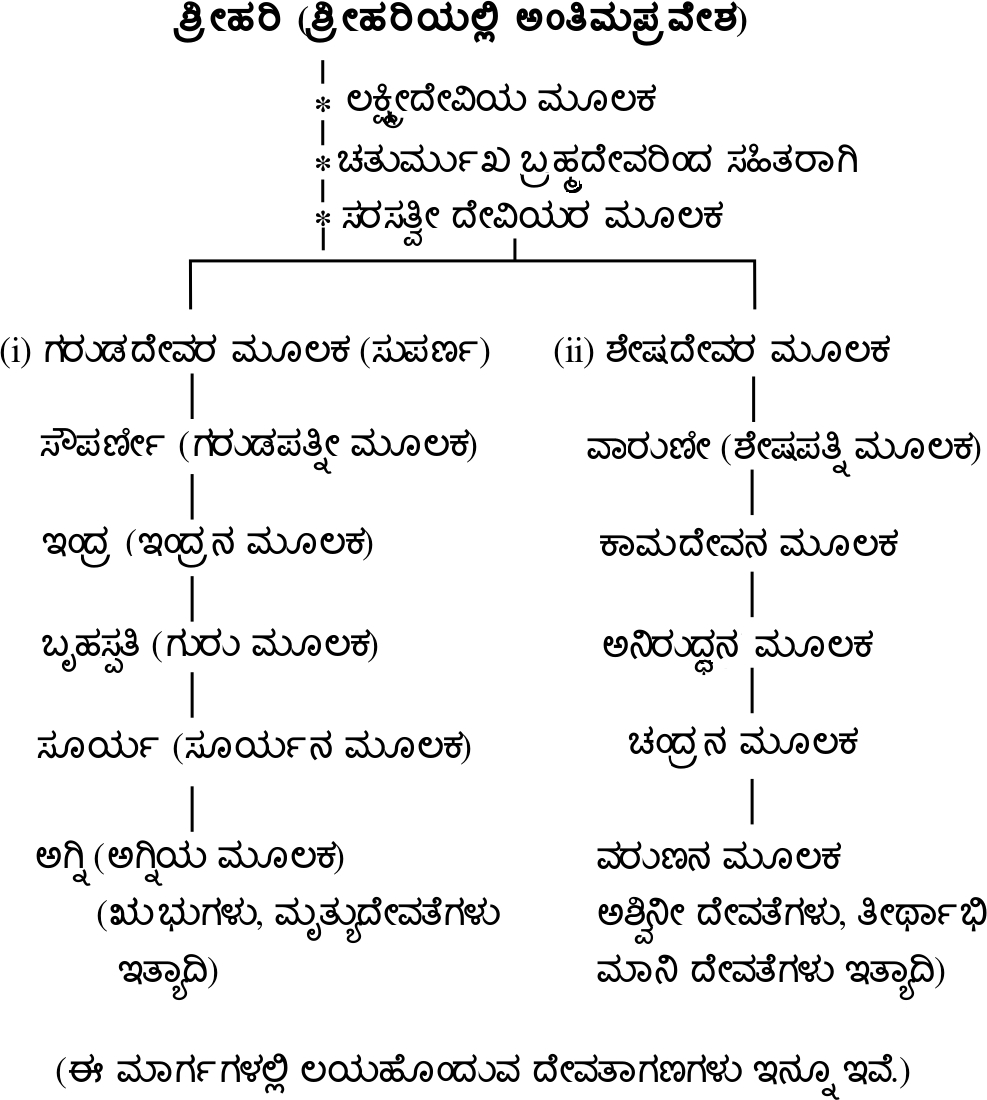
\includegraphics[scale=.85]{images/fig2.jpg}
\end{figure}

(ಈ ಮಾರ್ಗಗಳಲ್ಲಿ ಲಯಹೊಂದುವ ದೇವತಾಗಣಗಳು ಇನ್ನೂ ಇವೆ.)

\textbf{(೩೯)} ಉಕ್ತರೀತ್ಯಾ ನರೋ ಭಗವಾನ್-ಮೇಲೆ ಹೇಳಿದ ರೀತಿಯಲ್ಲಿ ಷಡ್ಗುಣೈಶ್ವರ್ಯಪೂರ್ಣನಾದ ಶ‍್ರೀಹರಿಗೆ 'ನರ' ಎಂದು ಹೆಸರು. ತಸ್ಯೇದಂ ಸಂಬಂಧಿ ಸುದರ್ಶನಚಕ್ರಾದ್ಯಾಯುಧಜಾತಂ ನಾರಂ- ತಸ್ಯ=ಆ `ನರ' ನ, ಇದಂ ಸಂಬಂಧಿ (ಸಂಬಂಧ ಉಳ್ಳದ್ದು), 'ನಾರಂ'= ನಾರಂ ಎಂದು ಹೇಳಲ್ಪಡುತ್ತದೆ. (ಹೇಗೆಂದರೆ), ಸುದರ್ಶನ ಚಕ್ರಾದ್ಯಾಯುಧ\-ಜಾತಂ=ಸುದರ್ಶನಚಕ್ರವೇ ಮೊದಲಾದ ಆಯುಧ ಸಮೂಹಕ್ಕೆ ನಾರ ಎಂದು ಹೆಸರು. ತದೇವ ಅಯನಂ ಗತಿಸಾಧನಂ ಗಮನಸಾಧನಂ ವೈರಿನಿರಸನಸಾಧನಮಿತಿ ಯಾವತ್-ತದೇವ=ಅದೇ, (ನಾರ ಎಂದು ಹೇಳಲ್ಪಡುವ ಆಯುಧಸಮೂಹವೇ), ಅಯನಂ=ಗತಿಸಾಧನಂ=ಗಮನ\-ಸಾಧನ=ವೈರಿನಿರಸನಸಾಧನಮಿತಿ ಯಾವತ್=ಶತ್ರುಗಳ ಸಂಹಾರರೂಪಕವಾಗಿ ಅವರವರ ಗತಿಗಳಿಗೆ ಹೋಗಲು ಸಹಾಯಕವಾಗಿರುವುದರಿಂದ (ಅಯನಂ), ಯಸ್ಯ ಹರೇರಸೌ‌ ನಾರಾಯಣಃ\-- ಯಸ್ಯ. ಹರೇಃ=ಯಾವ ಹರಿಗೆ, ಸುದರ್ಶನಚಕ್ರಾದಿ ಆಯುಧಗಳು ಸಾಧನವಾಗಿವೆಯೋ, ಅಸೌ= ಅಂತಹವನು, ನಾರಾಯಣ.

ಯಥೋಕ್ತಂ=ಹೀಗೆ ಪ್ರಮಾಣವಿದೆ:-

\begin{verse}
\textbf{"ಚಕ್ರಂ ಯುಗಾಂತಾನಲತಿಗ್ಮನೇಮಿ ಭ್ರಮತ್ಸಮಂತಾತ್ ಭಗವತ್ಪ್ರಯುಕ್ತಂ~। ದಂದದ್ಧಿ ದಂದಗ್ಧರಿಸೈನ್ಯಮಾಶು"} ಇತ್ಯಾದಿ.
\end{verse}

\noindent
ಯಾಗಾಂತದ ಬೆಂಕಿಯಂತೆ ಇರುವ ತೀಕ್ಷ್ಣವಾದ ನೇಮಿ (Spokes) ಉಳ್ಳ, ಪರಮಾತ್ಮನಿಂದ ಬಿಡಲ್ಪಟ್ಟ ಸುದರ್ಶನವು ಎಲ್ಲ ಕಡೆಯಲ್ಲಿಯೂ ಸುತ್ತಿ ಶತ್ರುಸೈನ್ಯವನ್ನು ಶೀಘ್ರವಾಗಿಯೂ ಚೆನ್ನಾಗಿಯೂ ಸುಡುತ್ತದೆ.

\begin{center}
\textbf{ಶತ್ರುನಾಶಕರವಾದ ಸುದರ್ಶನ ಚಕ್ರವೇ ಮೊದಲಾದ ಆಯುಧಗಳನ್ನು ಹೊಂದಿರುವ ಕಾರಣದಿಂದ ನಾರಾಯಣ.}
\end{center}

\textbf{(೪೦)} ಉಕ್ತರೀತ್ಯಾ ನರೋ ಭಗವಾನ್-ಮೇಲೆ ಹೇಳಿದ ರೀತಿಯಲ್ಲಿ, ಭಗವಾನ್=\-ಷಡ್ಗುಣೈಶ್ವರ್ಯಪೂರ್ಣನಾದ ಶ‍್ರೀಹರಿಯು, ನರಃ='ನರ' ನೆಂದು ಕರೆಸಿಕೊಳ್ಳಲ್ಪಡುತ್ತಾನೆ. ತತ್ತ್ವಪ್ರತ್ಯೇನ ತತ್ಸಂಬಂಧಿ ತ್ವಾನ್ನಾರಾಃ ಬಹಿರಾವರಣ ಭೂತಾ ಆಪ-ತತ್ ಸೃಷ್ಟ ತ್ತೇನ=ಅದನ್ನು ಸೃಷ್ಟಿಮಾಡಿರುವ ಕಾರಣದಿಂದ, ತತ್ಸಂಬಂಧಿತ್ವಾತ್=ಅದರ ಸಂಬಂಧ ಹೊಂದಿರುವುದರಿಂದ, ಬಹಿರಾವರಣ ಭೂತಾಃ=ಬ್ರಹ್ಮಾಂಡದ ಹೊರಗಿನ ಆವರಣದಲ್ಲಿರುವ, ಆಪಃ=ಜಲವು, ನಾರಾಃ =`ನಾರಾ' ಎಂದು ಹೇಳಲ್ಪಡುತದೆ. (ಬ್ರಹ್ಮಾಂಡದ ಹೊರ ಆವರಣದಲ್ಲಿರುವ ಜಲವು ಶ‍್ರೀಹರಿಯಿಂದ ಸೃಷ್ಟಿಯಾದುದು ಎಂದು ತಾತ್ಪರ್ಯ) ತಾಸಾಂ ವಾಮಪಾದಾಂಗುಷ್ಠನಖಾದ್ ಬ್ರಹ್ಮಾಂಡಭೇದನದ್ವಾರಾಽಯನಂ ಬ್ರಹ್ಮಾಂಡಾಂತರಾಗಮನಂ ಯಸ್ಮಾತ್ ಭವತ್ಯಸೌ ತ್ರಿವಿಕ್ರಮರೂಪೀ ಭಗವಾನ್ ನಾರಾಯಣಃ-ತಾಸಾಂ=ಆ ನೀರಿಗೆ, ವಾಮಪಾದಾಂಗುಷ್ಠನಖಾತ್=ತನ್ನ ಎಡಗಾಲಿನ ಹೆಬ್ಬೆರಳಿನ ಉಗುರಿನಿಂದ, ಬ್ರಹ್ಮಾಂಡಛೇದನದ್ವಾರಾ=ಬ್ರಹ್ಮಾಂಡಖರ್ಪರವನ್ನು ಛೇದಿಸಿ ಮಾಡಿದ ದಾರಿಯಿಂದ \textbf{ಅಯನಂ}=ಬ್ರಹ್ಮಾಂಡಾಂತರಾಗಮನಂ= ಬ್ರಹ್ಮಾಂಡದ ಒಳಗೆ ಬರುವುದು, ಯಸ್ಮಾತ್=ಯಾರಿಂದ, ಭವತಿ= ಆಗುತ್ತದೆಯೋ, ಅಸೌ= ಅಂತಹವನು,\break ಭಗವಾನ್= ಷಡ್ಗುಣೈಶ್ವರ್ಯ ಪೂರ್ಣನಾದ, ತ್ರಿವಿಕ್ರಮ ರೂಪ ಧರಿಸಿರುವ, ನಾರಾಯಣ.

ಯಥೋಕ್ತಂ-"ತತ್ರ ಭಗವತಃ ಸಾಕ್ಷಾದ್ಯಜ್ಞಲಿಂಗಸ್ಯ ವಿಷ್ಣೋ ವಿಕ್ರಮತಃವಾಮಪಾದಾಂ\-ಗುಷ್ಠನಖನಿರ್ಭಿನ್ನೋರ್ಧ್ವಾಂಡಕಟಾಹವಿವರೇಣಾಂತಃ ಪ್ರವಿಷ್ಟಾಯಾ ಬಾಹ್ಯಜಲಧಾರಾ"\break ಇತ್ಯಾದಿ.

ತತ್ರ=ಅಲ್ಲಿ (ಬಲಿಚಕ್ರವರ್ತಿಯು ಯಾಗಮಾಡುತ್ತಿದ್ದ ಸ್ಥಳದಲ್ಲಿ), ಭಗವತಃ=ಷಡ್ಗುಣೈ\-ಶ್ವರ್ಯಪೂರ್ಣನಾದ, ಸಾಕ್ಷಾದ್ಯಜ್ಞಲಿಂಗಸ್ಯ=ಯಜ್ಞದ ಫಲಭೋಕ್ತೃವಾಗಿ ಎದುರಿಗೇ ಇರುವ, ವಿಷ್ಣೋಃ=( ತ್ರಿವಿಕ್ರಮರೂಪದಿಂದ ಇರುವ) ವಿಷ್ಣುವಿನ, ವಿಕ್ರಮತಃ=ಮಹಾಸಾಮರ್ಥ್ಯದಿಂದ, ವಾಮ ಪಾದಾಂಗುಷ್ಟನಖ=ಎಡಗಾಲಿನ ಹೆಬ್ಬೆಟ್ಟಿನ ಉಗುರಿನಿಂದ, ನಿರ್ಭಿನ್ನ= ಭೇದಿಸಲ್ಪಟ್ಟ ಉರ್ಧ್ವಾಂಡಕಟಾಹ=ಮೇಲಿನ ಬ್ರಹ್ಮಾಂಡ ಖರ್ಪರದಲ್ಲಿ ವಿವರೇಣ=ಉಂಟಾದ ದಾರಿಯಿಂದ, ಅಂತಃಪ್ರವಿಷ್ಟಾ-ಬ್ರಹ್ಮಾಂಡದ ಒಳಗೆ ಪ್ರವೇಶ ಮಾಡಿದ, ಯಾ=ಯಾವ, ಬಾಹ್ಯ ಜಲ\-ಧಾರಾ=ಬ್ರಹ್ಮಾಂಡದ ಹೊರಗಿದ್ದ ನೀರಿನ ಪ್ರವಾಹವು ಇವೇ ಮೊದಲಾಗಿ ಹೇಳಿದಂತೆ.

(ತ್ರಿವಿಕ್ರಮರೂಪವನ್ನು ಧರಿಸಿದ ವಾಮನದೇವರು ತನ್ನ ಒಂದು ಪಾದವನ್ನು ಇಟ್ಟು ಭೂಮಿಯನ್ನೆಲ್ಲ ಆಕ್ರಮಿಸಿದ ನಂತರ, ಎರಡನೇ ಪಾದವನ್ನು ಬ್ರಹ್ಮಾಂಡದಲ್ಲಿ ಇಡಲು ಆಗ ತ್ರಿವಿಕ್ರಮದೇವರ ಎಡಗಾಲಿನ ಹೆಬ್ಬೆರಳಿನ ಉಗುರಿನಿಂದ ಬ್ರಹ್ಮಾಂಡಖರ್ಪರವು ಸೀಳಿ, ಬ್ರಹ್ಮಾಂಡದ ಹೊರಗೆ ಇದ್ದ ಜಲವು ಬ್ರಹ್ಮಾಂಡದ ಒಳಗೆ ಪ್ರವಾಹರೂಪದಿಂದ ಬಂದು 'ಗಂಗಾ' ಎಂದು ಪ್ರಸಿದ್ಧಳಾದಳೆಂಬ ವಿಚಾರವು ಪುರಾಣೋಕ್ತ).

\newpage

\begin{center}
\textbf{ಬ್ರಹ್ಮಾಂಡದ ಬಹಿರಾವರಣದಲ್ಲಿದ್ದ ನೀರಿಗೆ ತ್ರಿವಿಕ್ರಮ ರೂಪ ಧರಿಸಿ ಎಡಗಾಲಿನ ಹೆಬ್ಬೆಟ್ಟಿನ ಉಗುರಿನಿಂದ ಬ್ರಹ್ಮಾಂಡಖರ್ಪರವನ್ನು ಸೀಳಿ ಒಳಗೆ ಬರಲು ದಾರಿಮಾಡಿಕೊಟ್ಟ ಕಾರಣದಿಂದ ನಾರಾಯಣ.}
\end{center}

\textbf{(೪೧)} ಉಕ್ತರೀತ್ಯಾ ನರೋ ಭಗವಾನ್=ಮೇಲೆ ಹೇಳಿದ ರೀತಿಯಲ್ಲಿ ಭಗವಾನ್=ಷಡ್ಗುಣೈ\-ಶ್ವರ್ಯಪೂರ್ಣನಾದ ಶ‍್ರೀಹರಿಯು, ನರಃ='ನರ' ಎಂದು ಕರೆಯಲ್ಪಡುತ್ತಾನೆ. ತಜ್ಜನ್ಯತಯಾ ತತ್ಸಂಬಂಧಿ ನಾರಂ ಪದಂತಜ್ಜನ್ಯತಯಾ=ಅವನಿಂದ ಹುಟ್ಟಿರುವ ಕಾರಣದಿಂದ, ತತ್ಸಂಬಂಧಿ=ಅವನ ಸಂಬಂಧ ಹೊಂದಿರುವುದರಿಂದ, ಪದ್ಯ=ಪದ್ಮವು (ಕಮಲಪುಷ್ಪ),\break ನಾರ-'ನಾರಂ' ಎಂದು ಹೇಳಲ್ಪಡುತ್ತದೆ. ('ನರ' ಸಂಬಂಧ ಉಳ್ಳದ್ದು 'ನಾರ'), ತಸ್ಯಾಯನಮಾಶ್ರಯಃ ಪದ್ಮನಾಭೋ ನಾರಾಯಣಃ -ತಸ್ಯ=ಆ ಪದ್ಮಕ್ಕೆ, ಅಯನಂ=ಆಶ್ರಯ=ಆಶ್ರಯ\-ನಾಗಿರುವುದರಿಂದ, ಪದ್ಮನಾಭಃ= ಪದ್ಮವನ್ನು ತನ್ನ ನಾಭಿಯಲ್ಲಿಟ್ಟುಕೊಂಡು ಅದಕ್ಕೆ ಆಶ್ರಯನಾಗಿರುವುದರಿಂದ, ನಾರಾಯಣಃ (ನಾರಂ ಅಯನಂ).

ಯಥೋಕ್ತಂ-"ಅಜಸ್ಯ ನಾಭಾವಿತಿ ಯಸ್ಯ ನಾಭೌರಭೂಚ್ಛ್ರುತೇಃ ಪುಷ್ಕರಂ ಲೋಕಸಾರಂ" ಇತಿ.

ಅಜಸ್ಯ ನಾಭೌ = ಜನನರಹಿತನಾದ ಪರಮಾತ್ಮನ ಹೊಕ್ಕಳಿನಲ್ಲಿ, ಇತಿ=ಹೀಗೆಂದು ಹೇಳುವ, ಶ್ರುತೇಃ=ವೇದದ (ವೇದದಿಂದ), ಯಸ್ಯ= ಯಾವ ಶ‍್ರೀಹರಿಯ, ನಾಭೇಃ=ಹೊಕ್ಕಳಿನ ದೆಸೆಯಿಂದ, ಲೋಕಸಾರಂ= ಹದಿನಾಲ್ಕು ಲೋಕಗಳಿಗೂ ಆಶ್ರಯಭೂತವಾದ, ಪುಷ್ಕರಂ=\-ಪದ್ಮವು, ಅಭೂತ್=ಹುಟ್ಟಿತು (ಎಂದು ತಿಳಿಯುತ್ತದೆ).

\begin{center}
\textbf{ತನ್ನ ನಾಭಿಯಿಂದ ಉತ್ಪನ್ನವಾದ ಪದ್ಮವನ್ನು ಧರಿಸಿರುವ ಕಾರಣದಿಂದ ನಾರಾಯಣ.}
\end{center}

\textbf{(೪೨)} ನರಶಬ್ದೋ ಜೀವಮಾತ್ರಪರಃ-'ನರ' ಶಬ್ದವು, ಜೀವಮಾತ್ರಪರಃ =ಜೀವನನ್ನು ಕುರಿತು ಹೇಳುವಂತಹುದು. ತಥಾ ಚ=ಹೀಗಿರುವುದರಿಂದ, ನರಾಣಾಮಿದಂ ನಾರಂ='ನರ'\-ನಿಗೆ ಸಂಬಂಧಪಟ್ಟಿರುವುದು \textbf{'ನಾರಂ'} ಎಂದೆನಿಸಿಕೊಳ್ಳುತ್ತದೆ. ಅಂದರೆ ಚತುರ್ದಶಸಂಖ್ಯೋ\-ಪೇತಂ ಭುವನಂ=ಹದಿನಾಲ್ಕು ಲೋಕಗಳು. ತಸ್ಯಾಯನಮಾಶ್ರಯೋ ವಿರಾಡ್ರೂಪೀ\break ಭಗವಾನ್ನಾ\-ರಾಯಣಃ- ತಸ್ಯ=ಆ ಹದಿನಾಲ್ಕು ಲೋಕಗಳಿಗೆ, (ನಾರಂ) \textbf{ಅಯನಂ}=ಆಶ್ರಯಂ\-=ಆಶ್ರಯ\-ನಾದವನು, ವಿರಾಡ್ರೂಪೀ=ವಿರಾಟ್ರೂಪ ಧರನಾದ, ಭಗವನ್ನಾರಾಯಣಃ =\-ಷಡ್ಗುಣೈಶ್ವರ್ಯಪೂರ್ಣನಾದ ನಾರಾಯಣ (ನಾರಂ ಅಯನಂ).

ಯಥೋಕ್ತಂ-"ಪಾತಾಲಮೇತಸ್ಯ ಹಿ ಪಾದಮೂಲಂ" ಇತ್ಯಾದಿ.

ಏತಸ್ಯ=ಈ ವಿರಾಟ್ರೂಪೀ ಪರಮಾತ್ಮನ, ಪಾದಮೂಲಂ=ಪಾದದ ಕೆಳಗಿನ ಭಾಗವು, ಪಾತಾಲಂ ಹಿ=ಪಾತಾಳಲೋಕದಲ್ಲಿಯೇ ಇದೆ ಎಂಬುದು ಪ್ರಸಿದ್ಧ ಇವೇ ಮೊದಲಾಗಿ ಹೇಳಲ್ಪಟ್ಟಿದೆ.

\begin{center}
\textbf{ವಿರಾಡ್ರೂಪದಿಂದ ಹದಿನಾಲ್ಕು ಲೋಕಗಳಿಗೆ ಆಶ್ರಯನಾಗಿರುವ ಕಾರಣದಿಂದ ನಾರಾಯಣ.}
\end{center}

\noindent
\textbf{ವಿಶೇಷಾಂಶ:\enginline{-}}

\begin{verse}
\textbf{(i) ಸ್ವಯಮೇಕಂ ಚ ಬಹುವತ್ ಪ್ರತ್ಯೇಕಂ ರೋಮಕೂಪಗಂ~।}\\\textbf{ರಮಾಬ್ರಹ್ಮಾದಿಕಂ ದೇಶ ಕಾಲಾವರ್ಣಾಂಡ ಪೂರ್ವಕಂ~।।}
\end{verse}

\vauthor{(ಸತ್ತತ್ವರತ್ನಮಾಲಾ)}

ರಮಾಬ್ರಹ್ಮಾದಿ ಸಕಲ ಚೇತನಸಮೂದಾಯವನ್ನೂ ಆಕಾಶ, ಕಾಲ ಸಹಿತ ಬ್ರಹ್ಮಾಂಡವನ್ನೂ ತನ್ನ ರೋಮಕೂಪಗಳಲ್ಲಿ ತಾನೊಬ್ಬನೇ (ಇತರರ ಸಹಾಯವಿಲ್ಲದೇ) ಆಶ್ರಯಕೊಟ್ಟು ಧರಿಸಿರುತ್ತಾನೆ.

\begin{verse}
\textbf{(ii) ಮಯಾ ತತಮಿದಂ ಸರ್ವಂ ಜಗದವ್ಯಕಮೂರ್ತಿನಾ~।}\\\textbf{ಮತ್ಸ್ಥಾನಿ ಸರ್ವಭೂತಾನಿ ನ ಚಾಹಂ ತೇಷ್ಟವಸ್ಥಿತಃ~।।}
\end{verse}

ಅವ್ಯಕ್ತನಾದ ನನ್ನಿಂದ ಈ ಸಮಸ್ತ ಜಗತ್ತು ವ್ಯಾಪಿಸಲ್ಪಟ್ಟಿರುತ್ತದೆ. ಸಮಸ್ತ ಜೀವಜಡಾತ್ಮಕ ಭೂತಗಳು ನನ್ನನ್ನು ಆಶ್ರಯಿಸಿಕೊಂಡಿವೆ. ಆದರೆ ನಾನು ಅವುಗಳ ಆಶ್ರಯದಲ್ಲಿಲ್ಲ.

\textbf{(೪೩)} ನರಾಣಾಮಿದಂ ನಾರಂ-ನರಾಣಾಂ=ಚೇತನರ, ಇದಂ= ಸಂಬಂಧಉಳ್ಳದ್ದು ನಾರಂ=ನಾರಂ ಎಂದು ಹೇಳಲ್ಪಡುತ್ತದೆ. ಅಂದರೆ, ಜಾಗ್ರದಾದ್ಯವಸ್ಥಾತ್ರಯಂ= ಚೇತನದ ಜಾಗ್ರತ್ ಮುಂತಾದ ಮೂರು ಅವಸ್ಥೆಗಳು (ಜಾಗ್ರತ್=ಎಚ್ಚರಿಕೆಯಿಂದ ಇದ್ದು ವ್ಯಾಪಾರಗಳನ್ನು ಮಾಡುವುದು, ಸುಷುಪ್ತಿ=ಗಾಢನಿದ್ರೆ, ಸ್ವಪ್ಪ=ಕನಸುಕಾಣುವುದು), ಪ್ರವರ್ತಕತಯಾ=ಈ ಮೂರು ಅವಸ್ಥೆಗಳನ್ನು ಚೇತನರಲ್ಲಿ ಪ್ರವರ್ತನೆಮಾಡುವುದರಿಂದ, ತದಯನತ್ವಾತ್=ಆ ಅವಸ್ಥೆಗಳಿಗೆ ಆಶ್ರಯನಾಗಿರುವುದರಿಂದ (ಅಯನಂ), ವಿಶ್ವಾದಿರೂಪೀ= "ವಿಶ್ವ" ಮುಂತಾದ ರೂಪಧರನಾದ (ವಿಶ್ವ, ತೈಜಸ, ಪ್ರಾಜ್ಞ) ಭಗವನ್ನಾರಾಯಣಃ=ಷಡ್ಗುಣೈಶ್ವರ್ಯ\-ಪೂರ್ಣನಾದ ನಾರಾಯಣ. (ನಾರಂ ಅಯನಂ)

\begin{center}
\textbf{ವಿಶ್ವಾದಿರೂಪಗಳಿಂದ ಜಾಗ್ರದಾದಿ ಅವಸ್ಥೆಗಳಿಗೆ ಪ್ರೇರಕನಾಗಿರುವ ಕಾರಣದಿಂದ ನಾರಾಯಣ.}
\end{center}

\noindent
\textbf{ವಿಶೇಷಾಂಶ:\enginline{-}}

ಜೀವರಲ್ಲಿ ಜಾಗ್ರದವಸ್ಥೆ, ಸ್ವಪ್ನಾವಸ್ಥೆ, ಸುಷುಪ್ತಿಗಳನ್ನು ಉಂಟುಮಾಡುವವನು\break ಶ‍್ರೀಹರಿಯೇ.

\begin{verse}
\textbf{(i) ಓಂ ಪರಾಭಿಧ್ಯಾನಾತ್ತು ತಿರೋಹಿತಂ ತತೋ ಹ್ಯಸ್ಯ ಬಂಧವಿಪರ್ಯಯೌ ಓಂ (೩\enginline{-}೨\enginline{-}೫)}
\end{verse}

ತತಃ=ಪರಮಾತ್ಮನದೆಸೆಯಿಂದ, ಅಸ್ಯ=ಜೀವನಿಗೆ, ಬಂಧವಿಪರ್ಯಯೌ= ಬಂಧಮೋಕ್ಷಗಳು (ಆಗುತ್ತವೆಯೋ), ಪರಾಭಿಧ್ಯಾನಾತ್ತು=(ಆ ಕಾರಣದಿಂದ) ಪರಮಾತ್ಮನ ಇಚ್ಛೆಯಿಂದಲೇ, ತಿರೋಹಿತಂ=ಸ್ವಪ್ನನಾಶವೂ ಆಗುತ್ತದೆ.

\noindent
\textbf{ಭಾಷ್ಯ-}

\begin{verse}
\textbf{ಸ್ವಪ್ನಾದಿಬುದ್ಧಿಕರ್ತಾ ಚ ತಿರಸ್ಕರ್ತಾ ಸ ಏವ ಚ~।}\\\textbf{ತದಿಚ್ಛಯಾ ಯತೋ ಹ್ಯಸ್ಯ ಬಂಧಮೋಕ್ಷೌ ಪ್ರತಿಷ್ಠಿತೌ~।।}
\end{verse}

\vauthor{- ಕೂರ್ಮಪುರಾಣ.}

ಯಾರಿಂದ ಈ ಜೀವನಿಗೆ ಸಂಸಾರದಲ್ಲಿ ಬಂಧ ಮತ್ತು ಅದರ ಬಿಡುಗಡೆಗಳು ಆಗುತ್ತ\-ವೆಯೋ, ಅವನ (ಪರಮಾತ್ಮನ) ಇಚ್ಛೆಯಿಂದಲೇ ಸ್ವಪ್ನಾದಿಗಳ ಮರೆ ಮತ್ತು ಸ್ವಪ್ನದ ಅನು\-ಭವವೂ ಸಹ ಆಗುತ್ತವೆ. ಅಂದರೆ, ಸ್ವಪ್ನದ ತಿಳಿವಳಿಕೆ ಕೊಡುವವನೂ ಅವನೇ, ಸ್ವಪ್ನದ ಪರಿಹಾರ ಮಾಡುವವನೂ ಅವನೇ, ಜೀವನಿಗೆ ಬಂಧಮೋಕ್ಷಗಳೂ ಸಹ ಅವನಿಂದಲೇ-ಅನ್ಯರಿಂದಲ್ಲ.

\begin{verse}
\textbf{(ii) ಓಂ ದೇಹಯೋಗಾದ್ವಾಸೋಽಪಿ ಓಂ (೩\enginline{-}೨\enginline{-}೬)}
\end{verse}

ದೇಹಯೋಗಾತ್ ವಾಸಃ ಅಪಿ=ದೇಹದಮೇಲಿನ ಅಭಿಮಾನದಿಂದ ಇರುವುದೆಂಬ\break ಜಾಗ್ರದವಸ್ಥೆಯೂ ಕೂಡ, (ಪರಾಭಿಧ್ಯಾನಾತ್) ಆ ಭಗವಂತನ ಇಚ್ಛೆಯಿಂದಲೇ-ಜಾಗೃದ\-ವಸ್ತಾಪ್ರವರ್ತಕನೂ ಸಹ ಶ‍್ರೀಹರಿಯೇ.

\textbf{ಭಾಷ್ಯ\enginline{-}ದೇಹಯೋಗೇನ ವಾಸೋ ಜಾಗ್ರದಪಿ ತತ ಏವ~। ಸ ಏವ ಜಾಗರಿತೇ ಸ್ಥಾಪಯತಿ ಸ ಸ್ವಪ್ನೇ ಸ ಪ್ರಭುಃ ತುರಾಷಾಟ್ ಸ ಏಕೋ ಬಹುಧಾ ಭವತಿ, ಇತಿ ಕೌಂಠರವ್ಯ ಶ್ರುತೇಃ\enginline{-}}

ದೇಹಾಭಿಮಾನದಿಂದ ಜಾಗ್ರದವಸ್ಥೆಯೂ ಸಹ ಆ ಪರಬ್ರಹ್ಮನಿಂದಲೇ; ಅವನೇ (ವಿಶ್ವರೂಪದಿಂದ) ಜಾಗ್ರದವಸ್ಥೆಯನ್ನು ಉಂಟುಮಾಡುತ್ತಾನೆ; ಅವನೇ ಸ್ವಪ್ನದಲ್ಲಿ ಇಡುತ್ತಾನೆ. ಅವನೇ ಸರ್ವಸಮರ್ಥನು, ಸರ್ವವನ್ನೂ ನಿಗ್ರಹಿಸುವವನು, ಅವನು ಒಬ್ಬನೇ ಅನೇಕ ರೂಪಗಳಿಂದ ಪ್ರಕಟಗೊಳ್ಳುತ್ತಾನೆ-ಹೀಗೆಂದು ಕೌಂಠರವ್ಯಶ್ರುತಿ ತಿಳಿಸುತ್ತದೆ.

\begin{verse}
\textbf{(i) ಓಂ ತದಭಾವೋ ನಾಡೀಷು ತಚ್ಛ್ರುತೇರಾತ್ಮನಿ ಹ ಓಂ (೩\enginline{-}೨\enginline{-}೭)}
\end{verse}

ನಾಡೀಷು=ನಾಡಿಗಳಲ್ಲಿ, (ಇರುವ), ಆತ್ಮನಿ=ಪರಮಾತ್ಮನು, (ಪ್ರವೇಶಿಸುತ್ತಿರಲು), ತದಭಾವಃ =ಜಾಗ್ರತ್ ಮತ್ತು ಸ್ವಪ್ನಾವಸ್ಥೆಗಳ ಅಭಾವವು (ಎಂದರೆ ಸುಷುಪ್ತಿ ಎಂಬ ಗಾಢನಿದ್ರಾ\-ವಸ್ಥೆಯು) ಉಂಟಾಗುತ್ತದೆ. ತತ್ ಶ್ರುತೇಃ =ಛಾಂದೋಗ್ಯಶ್ರುತಿಯು ಈ ರೀತಿ ಹೇಳುವುದರಿಂದ, ಹ=ಈ ಅರ್ಥವು ಯುಕ್ತವು.

\begin{verse}
\textbf{ಭಾಷ್ಯ\enginline{-}ಜಾಗ್ರತ್ಸ್ವಪ್ನಾಭಾವಃ ಸುಪ್ತಿಃ ನಾಡಿಸ್ಥೇ ಪರಮಾತ್ಮನಿ~। "ಅಸು ತದಾ ನಾಡೀಷು ಸುಪ್ತೋ ಭವತಿ~। ಸತಾ ಸೋಮ್ಯ ತದಾ ಸಂಪನ್ನೋ ಭವತಿ" ಇತಿ ಶ್ರುತೇಃ~।।}
\end{verse}

ಜಾಗ್ರತ್, ಸ್ವಪ್ನ ಇವುಗಳ ವಿರೋಧವಾದ ಗಾಢನಿದ್ರಾವಸ್ಥೆಯು (ಜೀವನಿಗೆ) ಪರಮಾತ್ಮನು ಸುಷುಮ್ನಾ ನಾಡಿಗಳಲ್ಲಿ ಇರುವಾಗ ಉಂಟಾಗುತ್ತದೆ. ಸೋಮಪಾನಕ್ಕೆ ಅರ್ಹನಾದವನೇ (ಶ್ವೇತಕೇತುವೇ), ಯಾವಾಗ ಸುಷುಮ್ನಾ ನಾಡಿಗಳಲ್ಲಿ ಪರಮಾತ್ಮನು ಪ್ರವೇಶಮಾಡುತ್ತಾ\-ನೆಯೋ ಆಗ ಜೀವನು ಗಾಢನಿದ್ರೆಯನ್ನು ಹೊಂದುತ್ತಾನೆ. ಆಗ ಆ ಜೀವನು ಸತ್ಯಶಬ್ದವಾಚ್ಯನಾದ ಪರಮಾತ್ಮನಿಂದ ಸಹಿತನಾಗಿ ಇರುತ್ತಾನೆ. (ಜೀವನು ನಾಡೀಸ್ಥ ಪರಮಾತ್ಮನನ್ನು ಆಲಂಗಿಸಿ\-ಕೊಳ್ಳುತ್ತಾನೆ; ಇದೇ ಗಾಢನಿದ್ರೆಯು).

\begin{verse}
\textbf{(iv) ಜಾಗ್ರತ್ ಸ್ವಪ್ನಸುಷುಪ್ತ್ಯಾದಿ ಸರ್ವಾವಸ್ಥಾ ಪ್ರವರ್ತಕಃ~।}\\\textbf{ತತ್ತಿರೋಧಾನಕರ್ತಾ ಚ ಸ್ವತ ಏವ ಪ್ರಬೋಧಕಃ~।।}
\end{verse}

\vauthor{(ಸತ್ತತ್ವರತ್ನಮಾಲಾ)}

ಜಾಗ್ರತ್, ಸ್ವಪ್ನ, ಸುಷುಪ್ತಿ ಇತ್ಯಾದಿ (ಮೂರ್ಛೆ, ಮರಣ, ಸಮಾಧಿ) ಅವಸ್ಥೆಗಳ ಪ್ರವರ್ತಕನೂ, ಮತ್ತು ಅಂತಹ ಅವಸ್ಥೆಗಳ ತಿರೋಧಾನಕರ್ತನೂ ಪರಮಾತ್ಮನೇ; ಎಲ್ಲ ಅವಸ್ಥೆಗಳಲ್ಲಿಯೂ ಸಮಸ್ತ ಕಾರ್ಯಪ್ರಚೋದಕನೂ ಅವನೇ, ಅನ್ಯರಲ್ಲ.

\textbf{(೪೪)} ನರಾಣಾಮಿದಂ ನಾರಂ-ನರಾಣಾಂ=ಚೇತನಸಮುದಾಯಕ್ಕೆ, ಇದಂ=ಸಂಬಂಧಿ\-ಸಿದುದು, ನಾರಂ=\textbf{'ನಾರಂ'} ಎಂದು ಹೇಳಲಾಗುತದೆ. ಚಕ್ಷುರ್ಮನೋಹೃದಯರೂಪಸ್ಥಾನ\-ತ್ರಯಂ ಚ ಹೇಗೆಂದರೆ, ಚಕ್ಷುಃ =ನೇತ್ರ, ಮನಃ =ಮನಸ್ಸು, ಹೃದಯ=ಹೃದಯ, ರೂಪ ಸ್ಥಾನತ್ರಯಂ=ರೂಪಗಳಿಂದ ಇರುವ ಮೂರು ಪ್ರದೇಶ (ಅಧಿಷ್ಠಾನ)ಗಳು (ಈ ಮೂರು ಸ್ಥಾನಗಳು ನಾರಂ-ಚೇತನಸಂಬಂಧಿ), ತದೇವಾಯನಮಾಶ್ರಯೋ, ತತ್ ಏವ=ಆ ಮೂರು ಸ್ಥಾನಗಳು, \textbf{ಅಯನಂ}=ಆಶ್ರಯಃ = ಆಶ್ರಯವು, ಯಸ್ಯ=ಯಾರಿಗೆ ಇದೆಯೋ, ಅಸೌ=ಅಂತಹವನು, ವಿಶ್ವಾದಿರೂಪೀ=ವಿಶ್ವ ಮೊದಲಾದ ರೂಪಗಳನ್ನುಳ್ಳ, ಭಗವಾನ್ನಾ\-ರಾಯಣಃ = ಷಡ್ಗುಣೈಶ್ವರ್ಯಪೂರ್ಣನಾದ ನಾರಾಯಣನು; ಆಶ್ರಯವು ಹೇಗೆಂದರೆ, ಜಾಗ್ರದಾದ್ಯವಸ್ಥಾಪ್ರವರ್ತನೆ=\-ಜಾಗ್ರತ್, ಸ್ವಪ್ನ, ಸುಷುಪ್ತಿ ಮೊದಲಾದ ಅವಸ್ಥೆಗಳ (ಚೇತನರಲ್ಲಿ) ಪ್ರವರ್ತಕನಾಗಿರುವುದರಿಂದ (ನಾರಂ ಅಯನಂ), ಅಸ್ಕಿನ್=ಈ, ಅರ್ಥದ್ವಯೇ=ಎರಡು ಬಗೆಯ ಅರ್ಥಗಳಲ್ಲಿ (ಆಶ್ರಯತ್ವ, ಪ್ರೇರಕತ್ವ), ಮಾಂಡೂಕ್ಯೋಪನಿಷದೇವ=ಮಾಂಡೂಕ್ಯೋಪನಿಷತ್ತೇ, ಪ್ರಮಾಣಂ ಇತಿ=ಪ್ರಮಾಣವೆಂದು, ಅವಗಂತವ್ಯಂ=ತಿಳಿಯಬೇಕು.

\begin{center}
\textbf{ವಿಶ್ವಾದಿರೂಪಗಳಿಂದ ಜಾಗ್ರದಾದಿ ಅವಸ್ಥೆಗಳನ್ನು ಉಂಟುಮಾಡಲು ಚಕ್ಷು ಮನಸ್ಸು, ಹೃದಯರೂಪಸ್ಥಾನಗಳಲ್ಲಿ ನೆಲಸಿರುವ ಕಾರಣದಿಂದ ನಾರಾಯಣ.}
\end{center}

\noindent
\textbf{ವಿಶೇಷಾಂಶ:\enginline{-}}

\begin{verse}
\textbf{(i) ಏತಸ್ಮಾಜ್ಜಾಯತೇ ಪ್ರಾಣೋ ಮನಃ ಸರ್ವೇಂದ್ರಿಯಾಣಿ ಚ~। ಅಗ್ನಿರ್ಮೂರ್ಧಾ ಚಕ್ಷುಷೀ ಚಂದ್ರಸೂರ್ಯೌ ದಿಶಃ ಶೋತ್ರೇ ವಾಗ್ವಿವೃತಾಶ್ಚ ವೇದಾಃ~। ವಾಯುಃ ಪ್ರಾಣೋ ಹೃದಯಂ ವಿಶ್ವಮಸ್ಯ ಪದ್ಭ್ಯಾಂ ಪೃಥಿವೀ ಹ್ಯೇಷ ಸರ್ವಭೂತಾಂತರಾತ್ಮಾ~।।}
\end{verse}

\vauthor{-ಮಾಂಡೂಕ್ಯೋಪನಿಷತ್}

ಪ್ರಾಣ, ಮನಸ್ಸು, ಎಲ್ಲ ಇಂದ್ರಿಯಗಳು ಇವನಿಂದ ಹುಟ್ಟುವುವು. ಅಗ್ನಿಯು, ಇವನ ಶಿರಸ್ಸು, ಚಂದ್ರಸೂರ್ಯರು ಇವನ ಕಣ್ಣುಗಳು, ದಿಕ್ಕುಗಳು ಕಿವಿಗಳು, ಇವನ ಕಂಠದಿಂದ ಉದ್ಯೋತಿದವಾದ ಅಮರವಾಣಿಯೇ ವೇದಗಳು, ವಾಯುವು ಇವನ ಪ್ರಾಣವು. ವಿಶ್ವವು ಇವನ ಹೃದಯ, ಇವನ ಪಾದಗಳ ಆಶ್ರಯದಲ್ಲಿ ಪೃಥ್ವಿಯು ಇರುವುದು, ಇವನು ಸಮಸ್ತ ಚೇತನರಲ್ಲಿ ಅಂತರಾತ್ಮನಾಗಿದ್ದಾನೆ. (ಸಮಸ್ತ ಇಂದ್ರಿಯಗಳೂ ಇವನಿಂದ ಹುಟ್ಟಿದವು; ಅವುಗಳಲ್ಲಿ ಇವನು ಉಪಸ್ಥಿತನಿದ್ದು ಇಂದ್ರಿಯಗಳ ವ್ಯಾಪಾರಗಳನ್ನು ನಿಯಂತ್ರಿಸುತ್ತಾನೆ ಎಂದು ತಾತ್ಪರ್ಯ).

\begin{verse}
\textbf{(ii) ಸ್ತೋತ್ರಂ ಚಕ್ಷುಃ ಸ್ಪರ್ಶನಂ ಚ ರಸನಂ ಫ್ರಾಣಮೇವ ಚ~।}\\\textbf{ಅಧಿಷ್ಠಾಯ ಮನಶ್ಚಾಯಂ ವಿಷಯಾನುಪಸೇವತೇ~।।}
\end{verse}

\vauthor{-ಗೀತಾ}

ಈ ಪರಮಾತ್ಮನು ಶ್ರೋತ್ರೇಂದ್ರಿಯ, ಚಕ್ಷುರಿಂದ್ರಿಯ, ತ್ವಗಿಂದ್ರಿಯ, ಜಿಹ್ವೇಂದ್ರಿಯ, ಘ್ರಾಣೇಂದ್ರಿಯ ಮತ್ತು ಮನಸ್ಸು ಇವುಗಳಲ್ಲಿದ್ದು, ಪ್ರೇರಕನಾಗಿ ಶುಭವಿಷಯಗಳನ್ನು ಅನುಭವಿಸುತ್ತಾನೆ (ಪರಮಾತ್ಮನು ಶುಭ ವಿಷಯಗಳನ್ನು ಮಾತ್ರವೇ ಭೋಗಿಸುತ್ತಾನಲ್ಲದೆ, ಅಶುಭ ವಿಷಯಗಳನ್ನು ಎಂದಿಗೂ ಅನುಭವಿಸುವುದಿಲ್ಲ).

\textbf{(೪೫)} ನರಾಣಾಂ ಇಮೇ= ಚೇತನಸಮುದಾಯಕ್ಕೆ ಸಂಬಂಧಪಟ್ಟವುಗಳು, ರಾಕ್ಷಸ\-ಬಾಧಾದ್ಯುಪದ್ರವಪರಿಹಾರಾದಿನೋಪಕಾರಕತಯಾ-ರಾಕ್ಷಸ= ರಾಕ್ಷಸರ, ಬಾಧಾದಿ=\break ತೊಂದರೆಯೇ ಮೊದಲಾದ, ಉಪದ್ರವ=ಸಂಕಟಗಳ, (ಕಷ್ಟಗಳ), ಪರಿಹಾರಾದಿನಾ=ಪರಿಹಾರ\-ಮಾಡುವುದೇ ಮೊದಲಾದ, ಉಪಕಾರಕತಯಾ= ಉಪಕಾರಮಾಡುವುದರಿಂದ, ತತ್ಸಂಬಂಧಿನಃ =ಅದಕ್ಕೆ (ಚೇತನ ವರ್ಗಕ್ಕೆ) ಸಂಬಂಧಪಟ್ಟವುಗಳಾದ, ರಾಮಾದ್ಯವತಾರಾಃ = "ರಾಮ" ಇತ್ಯಾದಿ ಅವತಾರಗಳ, \textbf{ನಾರಾಃ} = "ನಾರಾ'' ಎಂದು ಹೇಳಲ್ಪಡುತ್ತವೆ. ತೇಷಾಂ=ಆ ಅವತಾರಗಳ, ಕಾರ್ಯಾಂತೇ= ಕೆಲಸ ಮುಗಿದನಂತರ, \textbf{ಅಯನಂ}=ಆಶ್ರಯಃ =ಆಶ್ರಯನಾದವನು, ನಿಧಾನಮೇಕೀ ಭವನಾಧಿಕರಣಮಿತಿ ಯಾವತ್‌ ಏಕೀಭವನಾಧಿಕರಣಂ = ಐಕ್ಯವಾಗುವುದಕ್ಕೆ, ನಿಧಾನಂ ಇತಿ ಯಾವತ್=ಭದ್ರವಾದ ಆಶ್ರಯದಾತನಂತೆ ಇರುವ, ಪದ್ಮನಾಭರೂಪೀ ಭಗವಾನ್=ಪದ್ಮನಾಭರೂಪದಿಂದಿರುವ ಷಡ್ಗುಣೈಶ್ವರ್ಯಪೂರ್ಣನಾದ, ನಾರಾಯಣ. (ರಾಮ ಕೃಷ್ಣಾದಿ ಅವತಾರ ಕೃತ್ಯಗಳು ಮುಗಿದನಂತರ ಅವತಾರ ರೂಪಗಳು ಮೂಲರೂಪದೊಂದಿಗೆ ಐಕ್ಯವಾಗುವುದರಿಂದ, ಮೂಲರೂಪನಾದ ನಾರಾಯಣನು ಅವತಾರರೂಪಗಳಿಗೆ ಆಶ್ರಯನೆಂದು ಅಭಿಪ್ರಾಯ).

ಯಥೋಕ್ತಂ-

\begin{verse}
\textbf{"ಏತನ್ನಾನಾವತಾರಾಣಾಂ ನಿಧಾನಂ ಬೀಜಮವ್ಯಯಂ~।}\\\textbf{ಯಸ್ಯಾಂಶಾಂಶೇನ ಸೃಜ್ಯಂತೇ ದೇವತಿರ್ಯಕ್‌ನರಾದಯಃ''}
\end{verse}

ಯಸ್ಯ=ಯಾವ ಪರಮಾತ್ಮನ, ಅಂಶಾಂಶೇನ=ಅನೇಕ ಅಂಶಗಳಿಂದ, ದೇವ=ದೇವತೆಗಳು, ತಿರ್ಯಕ್=ಮೂಕಜಂತುಗಳು, ನರಾದಯಃ = ಮನುಷ್ಯರೇ ಮೊದಲಾದ ಚೇತನರು, ಸೃಜ್ಯಂತೇ=ಸೃಷ್ಟಿಸಲ್ಪಡುತ್ತಾರೆಯೋ, (ಅಂತಹ ಪರಮಾತ್ಮನ) ಏತತ್ ನಾನಾವತಾರಾಣಾಂ=ಈ ಅನೇಕ ಅವತಾರ ರೂಪಗಳ, ನಿಧಾನ=ಆಶ್ರಯಸ್ಥಾನವು, ಬೀಜಂ ಅವ್ಯಯಂ=ನಾಶರಹಿತವಾದ ಮೂಲರೂಪವು, (ನಾರಾಯಣ ರೂಪವು)-ಎಂದು ಹೇಳಲಾಗಿದೆ.

(ಬ್ರಹ್ಮದೇವರೇ ಮೊದಲಾದ ದೇವತೆಗಳಿಂದ ತೃಣಜೀವಿಪರ್ಯಂತ ಎಲ್ಲ ಚೇತನರ ಶರೀರಗಳಲ್ಲಿಯೂ ಇರುವ ಜೀವನು ಪರಮಾತ್ಮನ ಅಂಶಕ್ಕೆ ಸದೃಶನೇ ಎಂದರೆ ಜ್ಞಾನಾದಿ\-ಸ್ವರೂಪನೇ).

\begin{center}
\textbf{ರಾಮಾದಿ ಅವತಾರ ಕಾರ್ಯಗಳು ಮುಗಿದನಂತರ ಪದ್ಮನಾಭ ರೂಪವಾದ ಮೂಲರೂಪದಲ್ಲಿ ಐಕ್ಯವಾಗುವ ಕಾರಣದಿಂದ ನಾರಾಯಣ.}
\end{center}

\noindent
\textbf{ವಿಶೇಷಾಂಶ:\enginline{-}}

\begin{verse}
\textbf{ಮಮೈವಾಂಶೋ ಜೀವಲೋಕೇ ಜೀವಭೂತಃ ಸನಾತನಃ~।}
\end{verse}

\vauthor{-ಗೀತಾ}

ಚತುರ್ಮುಖಾದಿ ಜೀವರ ಶರೀರಗಳಲ್ಲಿ ಇರುವ ಅನಾದಿ ನಿತ್ಯನಾದ ಜೀವನು ನನ್ನ ಅಂಶಕ್ಕೆ ಸದೃಶನೇ ಎಂದರೆ ಅಂಶದಂತೆ ಜ್ಞಾನಾದಿ ಸ್ವರೂಪನೇ!

\textbf{(೪೬) ನರಾಣಾಂ ಸ್ವಸಹಾಯೇನ ಪಠತಾಮರ್ಭಕಾಣಾಮಯಂ ತತ್ವೋಪದೇಷ್ಟೃತಯಾ ಸಂಬಂಧೀ ಪ್ರಹ್ಲಾದೋ ನಾರಾಶಬ್ಧೇನೋಚ್ಯತೇ~।}

ಸ್ವಸಹಾಯೇನ=ತನ್ನ ಸಹಾಯದಿಂದ, ಪಠತಾಂ=ವ್ಯಾಸಂಗ ಮಾಡುತ್ತಿರುವ,\break ಅರ್ಭಕಾಣಾಂ ನರಾಣಾಂ= ಬಾಲಕರಿಗೆ (ನರರಿಗೆ), ತತ್ತೋಪದೇಷ್ಟೃತಯಾ=ಯಥಾರ್ಥ\-ಜ್ಞಾನೋಪದೇಶವನ್ನು ಮಾಡುವ ದೃಷ್ಟಿಯಿಂದ, ಅಯಂ=ಈ, ಪ್ರಹ್ಲಾದಃ =ಪ್ರಹ್ಲಾದನು, ನಾರಶಬ್ದನ \textbf{'ನಾರ'} ಎಂಬ ಶಬ್ದದಿಂದ, ಉಚ್ಯತೇ=ಹೇಳಲ್ಪಡುತ್ತಾನೆ. (ಇಲ್ಲಿ 'ನರ' ಎಂದರೆ ತನ್ನ ಸಹಪಾಠಿಗಳೆಂದು ಅರ್ಥ. ಅವರಿಗೆ ಜ್ಞಾನೋಪದೇಶದ ಕಾರಣದಿಂದ ಸಂಬಂಧ ಹೊಂದಿರುವುದರಿಂದ ಪ್ರಹ್ಲಾದನಿಗೆ, 'ನಾರ' ಎಂದು ಹೆಸರು). ತಸ್ಯಾಯನಂ ಆಶ್ರಯಃ = ಆ ಪ್ರಹ್ಲಾದನಿಗೆ ಅಯನಂ=ಆಶ್ರಯಃ = ಆಶ್ರಯನಾಗಿರುವವನು, ನೃಸಿಂಹರೂಪೀ ಭಗವನ್ನಾರಾಯಣ=ನರಸಿಂಹ ರೂಪದಿಂದ ಪ್ರಕಟನಾದ ಷಡ್ಗುಣೈಶ್ವರ್ಯ ಭರಿತನಾದ ನಾರಾಯಣ. ಪ್ರಸಿದ್ಧಂ ಚೈತತ್ಸಪ್ತಮಸ್ಕಂಧೆ=ಈ ವಿಷಯವು (ಪ್ರಹ್ಲಾದನಿಗೆ ನರಸಿಂಹ ದೇವರು ಆಶ್ರಯ ಎಂಬುದು) ಭಾಗವತ ಸಪ್ತಮಸ್ಕಂಧದಲ್ಲಿ ಪ್ರಸಿದ್ಧವಾಗಿದೆ.

ಬಾಲಕರಿಗೆ ಜ್ಞಾನೋಪದೇಶ ಸಂದರ್ಭದಲ್ಲಿ ಪ್ರಹ್ಲಾದನ ನುಡಿಯು:-

\begin{verse}
\textbf{"ಹಂತಾರ್ಭಕಾಃ ಮೇ ಶೃಣುತ ವಚೋ ವಃ ಸರ್ವತಃ ಶಿವಂ~।}\\\textbf{ವಯಸ್ಯಾನ್ಪಶ್ಯತ ಮೃತಾನ್ ಕ್ರೀಡಾಂಧಾ ಮಾ ಪ್ರಮಾದ್ಯಥ"~।।}
\end{verse}

ಹಂತ=ಅಯ್ಯೋ, ಅರ್ಭಕಾಃ=ಬಾಲಕರೇ, ವಃ=ನಮಗೆಲ್ಲ, ಸದ್ವತ= ಸಮಸ್ತವಾದ, ವಯಸ್ಯಾನ್=ಸಂಸಾರದಲ್ಲಿ ವೈರಾಗ್ಯ ಉತ್ಪಾದಿಸಿ ಪರಮ ಪುರುಷಾರ್ಥಕ್ಕೆ ಕಾರಣವಾದ, ಶಿವ=ಮಂಗಳಕರವಾದ, ವಚಃ=ಮಾತನ್ನು ಶೃಣುತ=ಕೇಳಿರಿ. ಮೃತಾನ್=ಸತ್ತವರನ್ನು, ಪಶ್ಯತ=ನೋಡಿರಿ. ಕ್ರೀಡಾಂಧಾಃ=ಆಟಪಾಟಗಳಲ್ಲಿಯೇ ಮಗ್ನರಾಗಿ ಮಾ ಪ್ರಮಾದ್ಯಥ= ಅಕಾರ್ಯವನ್ನು ಮಾಡಬೇಡಿರಿ.

(ಬಾಲಕರೆ, ಸಾಯುವವರನ್ನು ನೋಡಿರಿ; ಆಟಪಾಟಗಳಲ್ಲಿಯೇ ಕಾಲವನ್ನು ವ್ಯರ್ಥಮಾಡಬೇಡಿರಿ. ಪುರುಷಾರ್ಥಹೇತುವಾದ ಸಮಸ್ತ ಮಂಗಳಗಳನ್ನೂ ನಮಗೆಲ್ಲ ದೊರಕಿಸುವ ನನ್ನ ಉಪದೇಶದ ಮಾತನ್ನು ಕೇಳಿರಿ.)

ನರಸಿಂಹರೂಪದಿಂದ ಪ್ರಹ್ಲಾದನಿಗೆ ಆಶ್ರಯನಾಗಿರುವ ಕಾರಣದಿಂದ ನಾರಾಯಣ.

\textbf{(೪೭)} ನರೋ ಮುಖ್ಯವಾಯುಃ-ಮುಖ್ಯವಾಯುದೇವರಿಗೆ 'ನರ' ಎಂದು ಹೆಸರು. ತಸ್ಯೇದಂ ಸಂಬಂಧಿ-ಆ 'ನರ' ಶಬ್ದವಾಚ್ಯ ಮುಖ್ಯವಾಯು ದೇವರಿಗೆ ಸಂಬಂಧಪಟ್ಟಿರು\-ವಂತಹುದು, ಹನುಮದಾಖ್ಯಂ ರೂಪಂ-ಹನುಮಂತನೆಂಬ ಹೆಸರಿನ ರೂಪವು, ನಾರಂ='ನಾರ' ಎಂದು ಕರೆಯಲ್ಪಡುತ್ತದೆ. ತಸ್ಯ ಅಯನಂ ಆಶ್ರಯಃ =ಆ 'ನಾರ' ನೆಂಬ ಹನುಮಂತ ದೇವರಿಗೆ, ಅಯನಂ=ಆಶ್ರಯಃ =ಆಶ್ರಯದಾತನಾದುದರಿಂದ, ರಾಮ ರೂಪೀ ಭಗವಾನ್=ಶ‍್ರೀರಾಮರೂಪದಿಂದ ಇರುವ ಷಡ್ಗುಣೈಶ್ವರ್ಯಪೂರ್ಣನಾದವನು, ನಾರಾಯಣ (ನಾರಂ ಅಯನಂ)...

\begin{center}
\textbf{ರಾಮದೇವರ ರೂಪದಿಂದ ಹನುಮಂತ ದೇವರಿಗೆ ಆಶ್ರಯನಾದ ಕಾರಣದಿಂದ ನಾರಾಯಣ}
\end{center}

\noindent
\textbf{ವಿಶೇಷಾಂಶ:\enginline{-}}

(i) ಹನುಮಂತದೇವರ ಅಪಾರವಾದ ಅಸದೃಶವಾದ ಭಕ್ತಿಯನ್ನು ಕಂಡು ಶ‍್ರೀರಾಮಚಂದ್ರ\-ದೇವರು ತಮ್ಮನ್ನೇ ಅವರಿಗೆ ಕೊಟ್ಟುಬಿಟ್ಟರೆಂದು ಸುಮಧ್ವವಿಜಯದಲ್ಲಿ ಹೀಗೆ ವರ್ಣಿಸಲಾಗಿದೆ;

\begin{center}
\textbf{ಸ್ವಾತ್ಮಾನಮೇವೈಷ ದದೌ ಯದಸ್ಮೈ}
\end{center}

\noindent
ಇದರಿಂದ ಶ‍್ರೀರಾಮಚಂದ್ರದೇವರು ಹನುಮಂತದೇವರಿಗೆ ಎಷ್ಟರಮಟ್ಟಿಗೆ ಆಶ್ರಯರಾದರು ಎಂಬುದು ತಿಳಿಯುತ್ತದೆ.

(ii) ಶ‍್ರೀಮನ್ಮಹಾಭಾರತತಾತ್ಪರ್ಯ ನಿರ್ಣಯದಲ್ಲಿ ಶ‍್ರೀಮದಾನಂದತೀರ್ಥರು ಹೀಗೆ ಹೇಳಿದ್ದಾರೆ:-

\begin{verse}
\textbf{ರಾಮೋಪಿ ನಾನ್ಯದನುದಾತುಮಮುಷ್ಯ ಯೋಗ್ಯಂ}\\\textbf{ಅತ್ಯಂತಭಕ್ತಿಭರಿತಸ್ಯ ವಿಲಕ್ಷ್ಯ ಕಿಂಚಿತ್~।}\\\textbf{ಸ್ವಾತಪ್ರದಾನಮಧಿಕಂ ಪವನಾತ್ಕಜಸ್ಯ}\\\textbf{ಕುರ್ವನ್ ಸಮಾಶ್ಲಿಷದಮುಂ ಪರಮಾಭಿತುಷ್ಟಃ~।।}
\end{verse}

\noindent
ಅಸದೃಶವಾದಭಕ್ತಿಭರಿತರಾದ ಹನುಮಂತದೇವರಿಗೆ ಯೋಗ್ಯವಾದ ಪ್ರತ್ಯುಪಕಾರಕವಾದ ವಸ್ತುವನ್ನು ಕಾಣದೇ ಶ‍್ರೀರಾಮಚಂದ್ರದೇವರು ವಾಯುಕುಮಾರರಾದ ಹನುಮಂತದೇವರಿಗೆ ಅತ್ಯಂತ ಸಂತೋಷದಿಂದ ತನ್ನ ಶರೀರದ ಆಲಿಂಗನದ ಸೌಭಾಗ್ಯವನ್ನು ದಯಪಾಲಿಸಿದರು.

(ii) ವಾಯುಸ್ತುತಿಯ ೨೧ನೇ ಶ್ಲೋಕದ ತಾತ್ಸರ್ಯವೂ ಸಹ ಹೀಗೆಯೇ ಇದೆ:-

ಸೀತಾದೇವಿಯವರಿಗೆ ಶ‍್ರೀರಾಮನ ಸಂದೇಶವನು ಒಯ್ದುದು, ಬ್ರಹ್ಮರುದ್ರ ವರಬಲದಿಂದ ಅವಧ್ಯರಾದ ರಾಕ್ಷಸರನ್ನು ಸಂಹರಿಸಿದುದು, ಇವೇ ಮೊದಲಾದ ಸೇವೆಯಿಂದ ಮೋಕ್ಷದಾತನಾದ ಶ‍್ರೀರಾಮನು ತೃಪ್ತನಾಗಿ ಬೇರೆ ಯಾರಿಗೂ ದೊರೆಯದ ಚತುರ್ಮುಖರೂಪ ಪ್ರಾಪ್ತಿಯಾಗುವಂತೆ ಶಿರಸ್ಸಿನಲ್ಲಿ ಕೈಯಿಟ್ಟು ಧನ್ಯನನ್ನಾಗಿ ಮಾಡಿ, ಮೋಕ್ಷದಲ್ಲಿ ಸಾಯುಜ್ಯಮೋಕ್ಷವನ್ನು ಅನುಗ್ರಹಿಸಿದನು.

\textbf{(೪೮)} ಉಕ್ತರೀತ್ಯಾ ನರೋ ವಾಯುಃ- ಮೇಲೆ ಹೇಳಿದ ರೀತಿಯಲ್ಲಿ ವಾಯುದೇವರಿಗೆ 'ನರ' ಎಂದು ಹೆಸರು. ತದ್ರೂಪಾಂತರತ್ತೇನ ತತ್ಸಂಬಂಧಿತ್ವಾತ್ ನರಾಣಾಂ ಅರ್ಜುನಾದಿರೂಪೇಣ ಉತ್ಪನ್ನಾನಾಂ ಇಂದ್ರಾದಿ ದೇವಾನಾಂ ತತ್ತೋಪದೇಶದ್ರಷೃತಯಾ ಗುರುತ್ತೇನ ತತ್ಸಂಬಂಧಿತ್ವಾತ್ ವಾ ನಾರೋ ಭೀಮಸೇನಃ-ತದ್ರೂಪಾಂತರತ್ವೇನ=ಬೇರೆ ರೂಪದಿಂದ, ತತ್ಸಂಬಂಧಿತ್ವಾತ್=ವಾಯುದೇವರಿಗೆ (ನರ ಶಬ್ದವಾಚ್ಯರಿಗೆ) ಸಂಬಂಧ ಹೊಂದಿರುವುದರಿಂದ, ಭೀಮಸೇನಃ = ಭೀಮಸೇನದೇವರು, ನಾರಃ = ನಾರ ಎಂದು ಹೇಳಲ್ಪಡುತ್ತಾರೆ. (ಇನ್ನೊಂದು ರೀತಿಯಲ್ಲಿಯೂ ಇದನ್ನೇ ಉಪಪಾದಿಸುತ್ತಾರೆ). ಅರ್ಜುನಾದಿ ರೂಪೇಣ= ಅರ್ಜುನನೇ ಮೊದಲಾದ ರೂಪದಿಂದ (ಅರ್ಜುನ, ಧರ್ಮರಾಯ, ನಕುಲ, ಸಹದೇವ ಇತ್ಯಾದಿ), ಉತ್ಪನ್ನಾನಾಂ=ಅವತಾರ ಮಾಡಿದ, ಇಂದ್ರಾದಿ ದೇವಾನಾಂ ನರಾಣಾಂ=ಮನುಷ್ಟರೂಪ\-ದಿಂದಿದ್ದ ಇಂದ್ರನೇ ಮೊದಲಾದ ದೇವತೆಗಳಿಗೆ, ತತ್ತೋಪದೇಶದ್ರಷ್ಟೃತಯಾ ಗುರುತ್ವೇನ=\-ಯಥಾರ್ಥಜ್ಞಾನವನ್ನು ಉಪದೇಶಮಾಡಿ ಗುರುಗಳ ಸ್ಥಾನದಲ್ಲಿ ಇದ್ದುದರಿಂದ, ತತ್ಸಂಬಂಧಿ\-ತ್ವಾತ್=ಅರ್ಜುನಾದಿರೂಪಗಳಲ್ಲಿದ್ದವರಿಗೆ (ಸಹೋದರ ಮುಂತಾದ) ಸಂಬಂಧಹೊಂದಿದ್ದರಿಂದ, ಭೀಮಸೇನ ದೇವರಿಗೆ \textbf{'ನಾರ'} ಎಂದು ಹೆಸರು. ತಸ್ಯ=ಆ ಭೀಮಸೇನದೇವರಿಗೆ ಅಯನತ್ವಾತ್=ಆಶ್ರಯನಾದುದರಿಂದ, ಭಗವಾನ್=ಷಡ್ಗುಣೈಶ್ವರಪೂರ್ಣನಾದ, ಕೃಷ್ಣರೂಪೀ=ಕೃಷ್ಣರೂಪದಿಂದ ಇರುವವನು ನಾರಾಯಣ. (ನಾರಂ ಅಯನ) ಭೀಮಸೇನದೇವರಿಗೆ ಆಶ್ರಯನು ಎಂದು ತಾತ್ಪರ್ಯ.

\begin{center}
\textbf{ಕೃಷ್ಣರೂಪದಿಂದ ಭೀಮಸೇನದೇವರಿಗೆ ಆಶ್ರಯನಾದ ಕಾರಣದಿಂದ ನಾರಾಯಣ.}
\end{center}

\noindent
\textbf{ವಿಶೇಷಾಂಶ:\enginline{-}}

ಅರ್ಜುನ ಮೊದಲಾದವರಿಗೆ ಭೀಮಸೇನದೇವರು ಶ‍್ರೀಕೃಷ್ಣನ ಸರ್ವೋತ್ತಮತ್ವ ಮುಂತಾದ ಮಹಾಮಹಿಮೆಗಳನ್ನು ಉಪದೇಶಮಾಡಿರುವುದು ಪ್ರಸಿದ್ಧವಾದ ವಿಷಯ. ಅಲ್ಲದೆ ಶ‍್ರೀಕೃಷ್ಣ\-ನಿಂದ ಮಾಡಲ್ಪಟ್ಟ ಗೀತೋಪದೇಶವು ಮುಖ್ಯವಾಗಿ ಅರ್ಜುನನ ರಥದ ಮೇಲಿದ್ದ ಕಪಿಧ್ವಜದ ಶ‍್ರೀಭೀಮಸೇನದೇವರನ್ನು ಕುರಿತದ್ದೇ. ಸರೋತ್ತಮನಾದ ಶ‍್ರೀಕೃಷ್ಣನಿಂದ ನೇರವಾಗಿ ಉಪದೇಶ ಪಡೆಯಲು ಅರ್ಜುನನು (ಇಂದ್ರಾಂಶ) ಅರ್ಹನಲ್ಲ. ಆದುದರಿಂದ ಮುಂದಿನ ಕಲಿಯುಗದಲ್ಲಿ ಭೀಮಸೇನದೇವರು ಆನಂದತೀರ್ಥರಾಗಿ ಅವತಾರಮಾಡಿದಾಗ, ಅರ್ಜುನನು ಎತ್ತಿನ ರೂಪದಿಂದ ಅವರ ಮುಂದೆ ಕುಳಿತುಕೊಂಡು, ಭಾಷ್ಯಾದಿ ಸಕಲ ಸಚ್ಛಾಸ್ತ್ರಗಳನ್ನೂ ಶ್ರವಣಮಾಡಿ ಮುಂದೆ ಆ ಎತ್ತೇ (ಇಂದ್ರಾಂಶರೇ) ಶ‍್ರೀಜಯತೀರ್ಥರೆಂಬ ಅಭಿಧಾನದಿಂದ ಅವತರಿಸಿ ಶ‍್ರೀಮದ್ವಾಚಾರ್ಯರ ಅನೇಕ ಪ್ರೌಢ ಗ್ರಂಥಗಳಿಗೆ ಜಗದ್ವಿಖ್ಯಾತವಾದ ಟೀಕಾಗಳನ್ನು ರಚಿಸಿದರೆಂಬುದು ಅತ್ಯಂತ ಪ್ರಸಿದ್ಧವಾದ ವಿಷಯ.

\textbf{(೪೯)} ನರೋ ವಾಯುಃ-ವಾಯುದೇವರಿಗೆ 'ನರ' ಎಂದು ಹೆಸರು. ತದ್ರೂಪಾಂತರತ್ಯೇನ ತತ್ಸಂಬಂಧಿತ್ವಾದ್ವಾನರಾಣಾಂ-ತದ್ರೂಪಾಂತರತ್ವೇನ=ಆ ವಾಯುದೇವರ (ನರ) ಇನ್ನೊಂದು ರೂಪದಿಂದ, ತತ್ಸಂಬಂಧಿತ್ವಾತ್ ವಾ=ಅದಕ್ಕೆ ಸಂಬಂಧಪಟ್ಟಿರುವುದರಿಂದಲೂ, ನರಾಣಾಂ=\break ಜನರಿಗೆ, ಕಲಿಕಾಲಕಲುಷಿತಾಂತಃಕರಣಾನಾಂ ಸಜ್ಜನಾನಾಂ= ಕಲಿಗಾಲದ ಪ್ರಭಾವದಿಂದ, ದೋಷಪೂರಿತವಾದ ಮನಸ್ಸು ಉಳ್ಳ ಸಜ್ಜನರಿಗೆ (ಮುಕ್ತಿಯೋಗ್ಯರಿಗೆ), ದಿವ್ಯಜ್ಞಾನೋಪದೇಶಾಯ=ಮುಕಿಪ್ರದವಾದ = ಯಥಾರ್ಥಜ್ಞಾನವನ್ನು ಉಪದೇಶ ಮಾಡಲು, ಅವತೀರ್ಣತ್ವೇನ= ಅವತಾರಮಾಡಿರುವುದರಿಂದ, ಗುರುತಯಾ=ಸಜ್ಜನರಿಗೆ ಗುರುಗಳಾದ ಕಾರಣದಿಂದ, ತತ್ಸಂಬಂಧಿತ್ವಾದ್ವಾ=ಅವರಿಗೆ ಸಂಬಂಧವನ್ನು ಹೊಂದಿರುವುದರಿಂದ, ನಾರಃ ಶ‍್ರೀಮದಾನಂದ\-ತೀರ್ಥಃ=ಶ‍್ರೀಮದಾನಂದತೀರ್ಥರು 'ನಾರ' ಎಂದು ಹೇಳಲ್ಪಡುತ್ತಾರೆ. ತಸ್ಮಾಯನಮಾ\-ಶ್ರಯಃ=ಆ ಆನಂದತೀರ್ಥರಿಗೆ, ಅಯನಂ=ಆಶ್ರಯಃ =ಆಶ್ರಯನಾಗಿರುವುದರಿಂದ,\break ಶ‍್ರೀವೇದವ್ಯಾಸರೂಪೀ ಭಗವನ್ನಾರಾಯಣಃ =ಶ‍್ರೀವೇದವ್ಯಾಸರೂಪದಿಂದಿರುವ ಷಡ್ಗುಣೈ\-ಶ್ವರ್ಯಪೂರ್ಣನಾದವನು ನಾರಾಯಣ. (ನಾರಂ ಅಯನಂ).

(ಶ‍್ರೀಮದಾನಂದತೀರ್ಥರು ವಾಯುದೇವರ (ನರ) ಅವತಾರಭೂತರಾದುದರಿಂದ\break ಅಂದರೆ ಮೂಲರೂಪದ ಸಂಬಂಧ ಹೊಂದಿರುವುದರಿಂದ, `ನಾರ' ಎಂದು ಹೇಳಲ್ಪಡುತ್ತಾರೆ. ಅಲ್ಲದೆ ಸಜ್ಜನರಿಗೆ (ಸಜ್ಜನರಿಗೆ ನರ ಎಂದು ಹೆಸರು). ಯಥಾರ್ಥಜ್ಞಾನವನ್ನು ಉಪದೇಶಮಾಡಲು ಅವತಾರಮಾಡಿರುವ ಕಾರಣದಿಂದಲೂ ಸಹ, ಅಂದರೆ 'ನರ' ರಿಗೆ ಗುರುತ್ತೇನ ಸಂಬಂಧ ಹೊಂದಿರುವುದರಿಂದಲೂ ಸಹ, ಶ‍್ರೀಮದಾನಂದತೀರ್ಥರಿಗೆ 'ನಾರ' ಎಂದು ಹೆಸರು).

\begin{center}
\textbf{ಶ‍್ರೀವೇದವ್ಯಾಸರೂಪದಿಂದ ಶ‍್ರೀಮದಾನಂದತೀರ್ಥರಿಗೆ ಆಶ್ರಯನಾದ ಕಾರಣದಿಂದ ನಾರಾಯಣ.}
\end{center}

\noindent
\textbf{ವಿಶೇಷಾಂಶ:\enginline{-}}

(i) ಶ‍್ರೀಮದಾಚಾರ್ಯರಿಗೆ ಶ‍್ರೀವೇದವ್ಯಾಸರು ಯಾವ ರೀತಿ ತಮ್ಮ ಪ್ರೀತ್ಯಾದರಗಳನ್ನು ಸೂಚಿಸಿ ಅನುಗ್ರಹಮಾಡಿದರೆಂಬ ವಿಚಾರವು ಸುಮಧ್ವವಿಜಯದಲ್ಲಿ ಹೀಗೆ ವರ್ಣಿಸಲಾಗಿದೆ:-

\begin{verse}
\textbf{ಅಮಿತಪ್ರಮತಿಂ ಶ್ರುತೀಶ್ವರಃ~।}\\\textbf{ಪರಿರೇಭೇ ಪರಿಗೃಹ್ಯ ತಂ ದ್ರುತಂ~।}\\\textbf{ಪ್ರಣಯಾಮೃತಪೂರ್ಣಮಾನಸಃ}\\\textbf{ಸ್ಮಿತವಕ್ತ್ರಃ ಪರಿಫುಲ್ಲಲೋಚನಃ~।।}
\end{verse}

ಶ‍್ರೀವೇದವ್ಯಾಸರು ಪ್ರೇಮದಿಂದ ತುಂಬಿದ ಮನಸ್ಸು ಉಳ್ಳವರಾಗಿದ್ದರು. ಮಂದಹಾಸದಿಂದಲೂ ತೆರೆದ ಕಣ್ಣುಗಳಿಂದಲೂ ಕೂಡಿದ ಅವರು ಶ‍್ರೀಮಧ್ವಾಚಾರ್ಯರನ್ನು ತ್ವರೆಯಿಂದ ತಬ್ಬಿಕೊಂಡರು.

\begin{verse}
\textbf{ಸಹಭೋಗಮನನ್ಯಲಭಭ್ಯಮಸ್ಮೈ}\\\textbf{ಹನುಮದ್ರೂಪವತೇ ದದೌ ಪುರಾ ಹಿ~।}\\\textbf{ಅನವೇಕ್ಷ್ಯ ಪರಂ ಸ್ವಭೀಷ್ಟಕರ್ತ್ರೇ}\\\textbf{ಪ್ರತಿದಾತುಂ ಹರಿರೈಧಯತ್ತಮೇವ~।}
\end{verse}

ಹನುಮಂತದೇವರಾಗಿ ಅವತಾರಮಾಡಿದ್ದಾಗ ಶ‍್ರೀರಾಮನ ರೂಪದಿಂದ ಸಹಭೋಗವೆಂಬ ಸೌಖ್ಯವನ್ನು ಕೊಟ್ಟಿದ್ದರು. ಮಧ್ವಾವತಾರದಲ್ಲಿ ತಮಗೆ ಪ್ರಿಯವಾದ ಕಾರ್ಯಗಳನ್ನು ಮಾಡಿರುವ ಇವರಿಗೆ ಬೇರೆ ಯಾವುದನ್ನೂ ಕೊಡಲು ಕಾಣದೆ ಆ ಸಹಭೋಗವನ್ನೇ ಇನ್ನೂ ಅಧಿಕಗೊಳಿಸಿದರು.

(ii) ಶ‍್ರೀವಾಯುದೇವರ ಹನುಮ, ಭೀಮ, ಮಧ್ವಾವತಾರಗಳು ಶ್ರುತಿ ಪ್ರಸಿದ್ದ. ಶ‍್ರೀಮದಾಚಾರ್ಯರೇ ತಾವು ಯಾರು, ಹಿಂದೆ ಯಾವ ಅವತಾರಗಳಿಂದ ಪರಮಾತ್ಮನ ಸೇವೆಯನ್ನು ಮಾಡಿದ್ದರು ಎಂಬ ವಿಷಯವನ್ನು "ಯಸ್ಯತ್ರೀಣ್ಯುದಿತಾನಿ ವೇದವಚನೇ...." ಈ ಶ್ಲೋಕದಿಂದ ಹೇಳಿರುತ್ತಾರೆ. ತ್ರಿವಿಕ್ರಮ ಪಂಡಿತಾಚಾರ್ಯರು ಈ ಮೂರು ರೂಪಗಳನ್ನು ಪ್ರತ್ಯಕ್ಷವಾಗಿ ನೋಡಿರುತ್ತಾರೆಂಬ ಐತಿಹ್ಯವಿದೆ. ಸುಮಧ್ವವಿಜಯದಲ್ಲಿ ಉಲ್ಲೇಖಿಸಿರುವ ಅನೇಕ ನಿದರ್ಶನಗಳಿಂದಲೂ (ಅನುಮಾನಗಳು) ಶ‍್ರೀಮದಾಚಾರ್ಯರು ಜೀವೋತ್ತಮರಾದ ವಾಯುದೇವರ ಅವತಾರಭೂತರೆಂದು ಸ್ಪಷ್ಟವಾಗುತ್ತದೆ. ವಾಯುಪುರಾಣದಿಂದಲೂ ಇದು ವೇದ್ಯವಾಗುತ್ತದೆ.

\begin{verse}
\textbf{ ಪ್ರಥಮೋ ಹನುಮಾನ್ನಾಮ ದ್ವಿತೀಯೋ ಭೀಮ ಏವ ಚ~।}\\\textbf{ಪೂರ್ಣಪ್ರಜ್ಞಸ್ಟೃತೀಯಸ್ತು ಭಗವತ್ಕಾರ್ಯಸಾಧಕಃ~।।}
\end{verse}

\noindent
ಮುಂತಾದ ವಾಕ್ಯಗಳೂ ಸಹ ಇದನ್ನೇ ಸಮರ್ಥಿಸುತ್ತವೆ.

(iii) ಎಲ್ಲ ಅವತಾರಗಳಲ್ಲಿಯೂ ಭಗವಂತನ ಸೇವೆಯನ್ನು ಅತ್ಯುತ್ತಮವಾಗಿ ಮಾಡಿದ ಇವರಿಗೆ ಪರಮಾತ್ಮನು ಆಲಿಂಗನಾದಿಗಳನ್ನು ಕೊಟ್ಟು ಆಶ್ರಯಭೂತನಾದುದರಲ್ಲಿ ಆಶ್ಚರ್ಯವೇನು?

\textbf{(೫೦)} ನರಾಣಾಂ ಸಜ್ಜನಾನಾಂ ದರ್ಶನವಂದನಾದಿನಾ ಪಾಪ ಪರಿಹಾರಕತ್ವೇನ ಉಪಕಾರತಯಾ ತತ್ಸಂಬಂಧಿತ್ವಾತ್ ನಾರಾಃ ಅಷ್ಟೌ ಗ್ರಾಮಾಣಃ-ನರಾಣಾಂ=ಸಜ್ಜನಾನಾಂ=ಸಜ್ಜನರ, ದರ್ಶನವಂದನಾದಿನಾ= ದರ್ಶನ ಮಾಡುವುದು, ನಮಸ್ಕಾರಾದಿಗಳನ್ನು ಮಾಡುವುದು ಈ ಕಾರ್ಯಗಳಿಂದ, ಪಾಪಪರಿಹಾರಕತ್ವೇನ=ಪಾಪಗಳನ್ನು ನಿವಾರಣೆಮಾಡುವುದರ ಮೂಲಕ, ಉಪಕಾರತಯಾ=ಉಪಕಾರ ಮಾಡುವುದರಿಂದ, ತತ್ಸಂಬಂಧಿತ್ವಾತ್=ಆ ಸಜ್ಜನರ ಸಂಬಂಧಹೊಂದಿರುವ ಕಾರಣದಿಂದ, ಅಷ್ಟೌಗ್ರಾವಾಣ=ಎಂಟು ವ್ಯಾಸಮುಷ್ಟಿಗಳೆಂಬ ಸಾಲಿಗ್ರಾಮಗಳಿಗೆ ನಾರಾಃ ಎಂದು ಹೆಸರು. ತಾನ್ಯೇವ ಅಯನಂ ಆಶ್ರಯಃ ಸನ್ನಿಧಾನತ್ವಾತ್ ಯಸ್ಯಾಸೌ\break ನಾರಾಯಣಃ-ತಾನಿ ಏವ=ಆ ಸಾಲಿಗ್ರಾಮಗಳೇ, ಯಸ್ಯ=ಯಾರಿಗೆ, ಸನ್ನಿಧಾನತ್ವಾತ್=\-ಸನ್ನಿಧಾನದ ಕಾರಣದಿಂದ, ಅಯನಂ=ಆಶ್ರಯಃ= ಆಶ್ರಯವಾಗಿ ಇವೆಯೋ, ಅಸೌ=\-ಅಂತಹವನು, ನಾರಾಯಣ (ನಾರಂ ಅಯನಂ).

ಯಥೋಕ್ತಂ ಸುಮಧ್ವವಿಜಯೇ-ಸುಮಧ್ವವಿಜಯದಲ್ಲಿ ಹೀಗೆ ಹೇಳಲಾಗಿದೆ-

\begin{verse}
\textbf{ಪ್ರಾಪ ಸ ನಾರಾಯಣತಃ ಶುದ್ಧಶಿಲಾತಪ್ರತಿಮಾಃ} \\\textbf{ಯಾಸು ಸ ಪದ್ಮಾಸಹಿತೋ ದೋಷ್ಯಹಿತಃ ಸನ್ನಿಹಿತಃ~।।}
\end{verse}

ಯಾಸು=ಯಾವ ಶಿಲಾರೂಪದವಿಗ್ರಹಗಳಲ್ಲಿ ದೋಷಿ=ಭಗವಂತನಲ್ಲಿ ದ್ವೇಷ ಮೊದಲಾದ ದೋಷ ಉಳ್ಳವರಿಗೆ, ಅಹಿತ=ಶತ್ರುವಾದ, ಸಃ=ಆ ನಾರಾಯಣನು, ಪದ್ಮಾಸಹಿತಃ=ಲಕ್ಷ್ಮೀ\-ಸಮೇತನಾಗಿ, ಸನ್ನಿಹಿತಃ= ಸನ್ನಿಧಾನದಿಂದ ಇರುವನೋ ಅಂತಹ, ಶುದ್ಧಶಿಲಾತ್ಮಪ್ರತಿಮಾಃ=\-ಪವಿತ್ರವಾದ ಶಿಲಾ ರೂಪದಿಂದ ಇರುವ ವಿಗ್ರಹಗಳನ್ನು ನಾರಾಯಣತಃ= ಶ‍್ರೀನಾರಾಯಣನ ಅವತಾರಭೂತರಾದ ಶ‍್ರೀವೇದವ್ಯಾಸದೇವರಿಂದ, ಸಃ=ಆ ಮಧ್ವಾಚಾರ್ಯರು, ಪ್ರಾಪ=\-ಪಡೆದರು.

ಬದರಿಕಾಶ್ರಮಕ್ಕೆ ಶ‍್ರೀಮದಾಚಾರ್ಯರು ಹೋಗಿದ್ದಾಗ ಶ‍್ರೀವೇದವ್ಯಾಸದೇವರು ಪರಮಪವಿತ್ರವಾದ ಎಂಟು ವ್ಯಾಸಮುಷ್ಟಿಗಳೆಂಬ ಪ್ರತಿಮಾರೂಪದಲ್ಲಿರುವ ಸಾಲಿಗ್ರಾಮಗಳನ್ನು ದಯಪಾಲಿಸಿದರು. (ಈ ವ್ಯಾಸಮುಷ್ಟಿಗಳು ಶ‍್ರೀಮದುತ್ತರಾದಿ ಮಠವೇ ಮುಂತಾದ ಆಚಾರ್ಯರ ಪರಂಪರಾನುಗತವಾಗಿ ಬಂದಿರುವ ಪೀಠಾಧಿಪತಿಗಳಿಂದ ಈಗಲೂ ಪೂಜಿಸಲ್ಪಡುತ್ತಿವೆ).

ಉಕ್ತಂ ಚ ವಾಯುಪುರಾಣೇ ಮಧ್ವಾವತರಣಖಂಡೇ ೨೯ ಅಧ್ಯಾಯೇ-ವಾಯು\-ಪುರಾಣದ ಮಧ್ಯಾವತರಣಖಂಡದಲ್ಲಿ ೨೯ನೇ ಅಧ್ಯಾಯದಲ್ಲಿ ಹೀಗೆ ಹೇಳಲಾಗಿದೆ:-

\begin{verse}
\textbf{"ನಿಶಮ್ಯ ತಸ್ಯ ವಾಕ್ಯಾನಿ ವ್ಯಾಸಃ ಸರ್ವಾಂತರಾತ್ಮಕಃ~।}\\\textbf{ಸ್ವಾಧಿಷ್ಟಾನಾನ್ ಪರಾನಷ್ಟೌ ಗ್ರಾವ್ಣೋ ನಾನಾಸುವರ್ಣಕಾನ್~।।}\\\textbf{ದದೌ ಸ್ತುತ್ವಾ ಪುನಸ್ತೋಷಾನ್ಮಧ್ವಃ ಪ್ರತಿಜಗಾಮ ಹ~।।”}
\end{verse}

ಸರ್ವಾಂತರಾತ್ಮಕಃ=ಸಮಸ್ತರಲ್ಲಿಯೂ ಅಂತರಾತ್ಮರಾದ, ವ್ಯಾಸಃ= ಶ‍್ರೀವೇದವ್ಯಾಸರು, ತಸ್ಯ=ಆ ಮಧ್ವರ, ವಾಕ್ಯಾನಿ=ಮಾತುಗಳನ್ನು, ನಿಶಮ್ಯ= ಕೇಳಿ, ನಾನಾಸುವರ್ಣಕಾನ್=ಅನೇಕ ಚಿನ್ನದ ನಾಣ್ಯಗಳನ್ನೂ, ಸ್ವಾಧಿಷ್ಠಾನ್= ತನ್ನ ಸನ್ನಿಧಾನದಿಂದ ಕೂಡಿರುವ, ಪರಾನ್=ಪವಿತ್ರ\-ವಾದ, ಅಷ್ಟೌಗ್ರಾವ್ಣಃ= ಎಂಟು ಶಿಲಾಪ್ರತಿಮೆಗಳನ್ನು (ಶಿಲಾಪ್ರತಿಮೆಯಂತಿರುವ ಸಾಲಿಗ್ರಾಮಗಳನ್ನು), ದದೌ=ಕೊಟ್ಟರು. ಮಧ್ವಃ=ಶ‍್ರೀಮಧ್ವಾಚಾರ್ಯರು, ಪುನಃ= ತಿರುಗಿ, ಸುತ್ವಾ\break =ಶ‍್ರೀವೇದವ್ಯಾಸರನ್ನು ಸ್ತೋತ್ರಮಾಡಿ, ತೋಷಾತ್= ಸಂತೋಷದಿಂದ, ಪ್ರತಿಜಗಾಮ=\break ಹಿಂತಿರುಗಿದರು. ಹ=ಇದು ಪ್ರಸಿದ್ದ.

(ಸುಮಧ್ವವಿಜಯದಲ್ಲಿ ನಾರಾಯಣದೇವರಿಂದ ಪಡೆದರು ಎಂದು ಹೇಳಿದೆ. ವಾಯುಪುರಾಣದಲ್ಲಿ ವೇದವ್ಯಾಸರಿಂದ ಪಡೆದರು ಎಂದಿದೆ. ಇದರಿಂದ ಸಾಕ್ಷಾತ್ ನಾರಾಯಣನೇ\break ವೇದವ್ಯಾಸರೆಂದು ಸ್ಪಷ್ಟ. ಕೆಲವರು ಹೇಳುವಂತೆ ವೇದವ್ಯಾಸರು ಒಬ್ಬ ಸಾಮಾನ್ಯ ಋಷಿಯಲ್ಲ).

\begin{center}
\textbf{ನರನಾರಾಯಣ ರೂಪದಿಂದ ಶ‍್ರೀಮದಾನಂದತೀರ್ಥರಿಗೆ ಕೊಟ್ಟ ಎಂಟು ವ್ಯಾಸಮುಷ್ಟಿಗಳೆಂಬ ಸಾಲಿಗ್ರಾಮದಲ್ಲಿ ತನ್ನ ಸನ್ನಿಧಾನವಿರುವ ಕಾರಣದಿಂದ ನಾರಾಯಣ.}
\end{center}

\textbf{(೫೧)} ನರಾಣಾಂ ಭೋಕ್ತೃಣಾಂ ಸಮೂಹಃ ನಾರಃ-ನರಾಣಾಂ= ಭೋಕೃಣಾಂ=ಭೋಜನ\-ಮಾಡುವ ಜನರ, ಸಮೂಹಃ=ಗುಂಪು, ನಾರಃ= ನಾರ ಎಂದು ಹೇಳಲ್ಪಡುತ್ತದೆ. ಸ ಏವ ಅಯನಂ ಸನ್ನಿಧಾನಸ್ಥಾನಂ ಯಸ್ಯಪ್ರದ್ಯುಮ್ನಸಂಕರ್ಷರೂಪಿಣಃ ಭಗವತಃ ಸಃ ನಾರಾ\-ಯಣಃ-ಸ ಏವ= ಆ ಭೋಜನಮಾಡುವ ಜನರ ಸಮೂಹವೇ, ಯಸ್ಯ ಭಗವತಃ=ಯಾವ ಷಡ್ಗುಣೈಶ್ವರ್ಯ ಪೂರ್ಣನಾದ, ಪ್ರದ್ಯುಮ್ನ ಸಂಕರ್ಷಣ ರೂಪಿಣಃ= ಪ್ರದ್ಯುಮ್ನ, ಸಂಕರ್ಷಣ ರೂಪಗಳಿಂದ, ಸನ್ನಿಧಾನಸ್ಥಾನಂ=ಸನ್ನಿಧಾನವಿರುವ ಪ್ರದೇಶವೋ (ಅಯನಂ=ಆಶ್ರಯಃ), ಸಃ=ಅವನು ನಾರಾಯಣ. (ಭೋಜನಮಾಡುವಾಗ ಚೇತನರಲ್ಲಿ ಪ್ರದ್ಯುಮ್ನ ಸಂಕರ್ಷಣರೂಪಗಳಿಂದ ಇದ್ದು, ತಾನೇ ಭೋಕ್ತೃವಾಗಿ, ಆಹಾರವನ್ನು ಸ್ವೀಕರಿಸುತ್ತಾನೆಂದು ತಾತ್ಪರ್ಯ) (ನಾರಂ ಆಯನಂ).

ಯಥೋಕ್ತಂ-ಹೀಗೆ ಪ್ರಮಾಣದಲ್ಲಿ ಹೇಳಲಾಗಿದೆ-

\begin{verse}
\textbf{"ಸಂಕರ್ಷಣಶ್ಚ ಪ್ರದ್ಯುಮ್ನಸ್ತತ್ರ ಭೋಕ್ತೃಷು ಸಂಸ್ಥಿತೌ~।"} ಇತಿ
\end{verse}

\noindent
ಭೋಜನಮಾಡುವ ಜನರಲ್ಲಿ ಸಂಕರ್ಷಣ ಮತ್ತು ಪ್ರದ್ಯುಮ್ನ ಎಂಬ ರೂಪಗಳು ಇರುತ್ತವೆ.

\begin{center}
\textbf{ಭೋಕ್ತೃಗಳಲ್ಲಿ ಸಂಕರ್ಷಣ ಪ್ರದ್ಯುಮ್ನರೂಪಗಳಿಂದ ಸನ್ನಿಧಾನದಿಂದಿರುವ ಕಾರಣದಿಂದ ನಾರಾಯಣ.}
\end{center}

\textbf{(೫೨)} ನರಾಣಾಮಿದಂ ಭೋಜ್ಯಮನ್ನಾದಿಜಾತಂ ನಾರಂ= ನರಾಣಾಂ=ಚೇತನಸಮು\-ದಾಯಕ್ಕೆ, ಇದಂ=ಸಂಬಂಧಪಟ್ಟಿದ್ದು, ಅಂದರೆ ಭೋಜ್ಯಂ =ತಿನ್ನಲ್ಪಡುವ, ಅನ್ನಾದಿ\-ಜಾತಂ=\break ಅನ್ನವೇ ಮೊದಲಾದ ಆಹಾರಗಳ ಸಮೂಹಗಳು, ನಾರಂ=ನಾರ ಎಂದೆನಿಸಿಕೊಳ್ಳುತ್ತವೆ. ತದೇವ ಅಯನಂ. ಸನ್ನಿಧಾನಸ್ಥಾನಂ ಯಸ್ಯ ನಾರಾಯಣಾನಿರುದ್ಧರೂಪಸ್ಯ ಹರೇಃ ಸ\break ನಾರಾಯಣಃ-ತತ್ ಏವ=ಆ ಅನ್ನಾದಿ ಆಹಾರ ಸಮೂಹವೇ (ನಾರಂ), ಯಸ್ಯ-ಯಾರ, ನಾರಾಯಣಾನಿರುದ್ಧರೂಪಸ್ಯ=ನಾರಾಯಣ ಮತ್ತು ಅನಿರುದ್ಧರೂಪಗಳನ್ನು ಹೊಂದಿರುವ, ಹರೇಃ-ಪರಮಾತ್ಮನ, ಸನ್ನಿಧಾನ ಸ್ಥಾನಂ=ತನ್ನ ಸನ್ನಿಧಾನವನ್ನಿಡಲು ಸ್ಥಳವಾಗಿದೆಯೋ, ಸಃ=\break ಅವನು ನಾರಾಯಣ.

(ನಾವು ಸ್ವೀಕರಿಸುವ ಆಹಾರಪದಾರ್ಥಗಳಲ್ಲಿ ಶ‍್ರೀಹರಿಯು ನಾರಾಯಣ ಮತ್ತು ಅನಿರುದ್ಧ ರೂಪಗಳಿಂದ ಸನ್ನಿಹಿತನಾಗಿರುತ್ತಾನೆಂದು ತಾತ್ಪರ್ಯ).

ಯಥೋಕ್ಕಂ-ಹೀಗೆ ಹೇಳಲಾಗಿದೆ-

\begin{verse}
\textbf{"ನಾರಾಯಣಾನಿರುದ್ಧೌ ತು ಭೋಜ್ಯವಸ್ತುಷು ಸಂಸ್ಥಿತೌ"} ಇತಿ-
\end{verse}

\noindent
ನಾವು ತಿನ್ನುವ ವಸ್ತುಗಳಲ್ಲಿ ನಾರಾಯಣ, ಅನಿರುದ್ಧ ರೂಪಗಳಿವೆ.

\begin{center}
\textbf{ಭೋಜ್ಯಪದಾರ್ಥಗಳಲ್ಲಿ ನಾರಾಯಣ, ಅನಿರುದ್ಧರೂಪಗಳಿಂದಿರುವ ಕಾರಣದಿಂದ ನಾರಾಯಣ.}
\end{center}

\textbf{(೫೩)} ನರಾಣಾಂ ಸಂಬಂಧಿ ನಾರೋ ಭುಕ್ತಾನ್ನಪಚನೇನೋದರೇ ಪುನರವಕಾಶಃ-\-ನರಾಣಾಂ ಸಂಬಂಧಿ=ಚೇತನರ ಸಮೂಹಕ್ಕೆ ಸಂಬಂಧಪಟ್ಟಿದುದು, ನಾರಃ =ನಾರ ಎಂದು ಹೇಳಲ್ಪಡುತ್ತದೆ; ಭುಕ್ತಾನ್ನ =ನಾವು ತಿಂದಿರುವ ಆಹಾರವನ್ನು ಪಚನೇನ=ಜೀರ್ಣವಾಗುವಂತೆ ಮಾಡಲು, ಉದರೇ=ನಮ್ಮ ಹೊಟ್ಟೆಯಲ್ಲಿ (ಜಠರದಲ್ಲಿ), ಪುನಃ ಅವಕಾಶಃ=ಸಾಕಷ್ಟುಸ್ಥಳ (ಬೇಕು). ತಸ್ಯ ದಾತೃತಯಾ ಅಯನಮಾಶ್ರಯೋ ವಾಸುದೇವರೂಪೀ ಭಗವಾನ್ನಾರಾಯಣಃ-ತಸ್ಯ ದಾತೃತಯಾ= ಅಂತಹ ಸ್ಥಳವನ್ನು ಕೊಡುವುದರ ಮೂಲಕ, ಅಯನಂ=ಆಶ್ರಯಃ=\break ಆಹಾರದ ಪಚನಕ್ಕೆ ಆಶ್ರಯನಾದುದರಿಂದ, ವಾಸುದೇವರೂಪೀ=ವಾಸುದೇವರೂಪಉಳ್ಳ (ಈ ರೂಪದಿಂದ ಸ್ಥಳಾವಕಾಶ ಮಾಡಿಕೊಡುತ್ತಾನೆ) ಭಗವಾನ್=ಷಡ್ಗುಣೈಶ್ವರ್ಯಪೂರ್ಣನಾದ\-ವನು, ನಾರಾಯಣ, (ನಾರಃ ಅಯನಂ).

ಯಥೋಕ್ತಂ-ಹೀಗೆ ಹೇಳಲಾಗಿದೆ-

\begin{verse}
\textbf{"ಅವಕಾಶಪ್ರದೋ ನಿತ್ಯಂ ವಾಸುದೇವೋ ನಭಃಸ್ಥಿತಃ"} ಇತಿ.
\end{verse}

ವಾಸುದೇವಃ=ವಾಸುದೇವರೂಪದಿಂದಿರುವ ಪರಮಾತ್ಮನು, ನಿತ್ಯಂ= ಯಾವಾಗಲೂ, ನಭಃ ಸ್ಥಿತಃ=ಜಠರಾಕಾಶಾದಿಗಳಲ್ಲಿದ್ದು, ಅವಕಾಶಪ್ರದಃ= ಆಹಾರವು ಪಚನವಾಗಲು\break ಸಹಾಯಕನಾಗಿರುತ್ತಾನೆ.

\begin{center}
\textbf{ವಾಸುದೇವರೂಪದಿಂದ ಪಚನಕ್ಕೆ ಅವಕಾಶಪ್ರದನಾದುದರಿಂದ ನಾರಾಯಣ.}
\end{center}

\noindent
\textbf{ವಿಶೇಷಾಂಶ:\enginline{-}}

ಮೇಲೆ ಹೇಳಿದ ಪ್ರಮೇಯವನ್ನೇ ಜ್ಞಾನಿಗಳಾದ ಶ‍್ರೀ ಜಗನ್ನಾಥದಾಸರು ಹರಿಕಥಾಮೃತಸಾರದಲ್ಲಿ ಈ ರೀತಿ ನಿರೂಪಿಸಿರುತ್ತಾರೆ:-

\begin{verse}
\textbf{ನಿರುಪಮಾನಂದಾತ್ಮ ಹರಿ ಸಂ}\\\textbf{ಕರುಷಣ ಪ್ರದ್ಯುಮ್ನ ರೂಪದಿ}\\\textbf{ಇರುತಿಹನು ಭೋಕ್ತೃಗಳೊಳಗೆ ತಚ್ಛಕ್ತಿದನುಯೆನಿಸಿ~।}\\\textbf{ಕರೆಸುವನು ನಾರಾಯಣನಿರು}\\\textbf{ದ್ದೆರಡು ನಾಮದಿ ಭೋಜ್ಯವಸ್ತುಗ}\\\textbf{ನಿರುತ ತರ್ಪಕನಾಗಿ ತೃಪ್ತಿಯನೀವ ಚೇತನಕೆ~।।}\\\textbf{ವಾಸುದೇವನು ಒಳಹೊರಗೆಯವ}\\\textbf{ಕಾಶ ಕೊಡುವ ನಭಸ್ಥನಾಗಿ ರ\enginline{-}}\\\textbf{ಮಾ ಸಮೇತ ವಿಹಾರ ಮಾಳ್ಪನು ಪಂಚರೂಪದಲಿ~।}
\end{verse}

\textbf{(೫೪)} ನರಾಣಾಂ ಸ್ಪರ್ಶನಪೂಜನಾದಿನಾ ಪಾವಿತ್ರ್ಯಕರ್ತೃತ್ವೇನ ತತ್ಸಂಬಂಧಿತ್ವಾತ್ ನಾರಾ ಸಾಲಿಗ್ರಾಮಶಿಲಾ-ನರಾಣಾಂ=ಸಜ್ಜನರಿಗೆ, ಸ್ಪರ್ಶನ ಪೂಜನಾದಿನಾ =ತನ್ನನ್ನು ಮುಟ್ಟುವುದರಿಂದಲೂ, ಪೂಜೆಯೇ ಮೊದಲಾದವುಗಳನ್ನು ಮಾಡುವುದರಿಂದಲೂ, ಪಾವಿತ್ರ್ಯಕರ್ತೃತ್ವೇನ= ಪವಿತ್ರರನ್ನಾಗಿ ಮಾಡುವ ಕಾರಣದಿಂದ, ತತ್ಸಂಬಂಧಿತ್ವಾತ್=ಆ ನರರಿಗೆ (ಸಜ್ಜನರಿಗೆ) ಸಂಬಂಧ ಹೊಂದಿರುವುದರಿಂದ, ಸಾಲಿಗ್ರಾಮಶಿಲಾ= ಸಾಲಿಗ್ರಾಮಶಿಲೆಯು, ನಾರಾ=ನಾರಾ ಎಂದು ಕರೆಯಲ್ಪಡುತ್ತದೆ.

\begin{verse}
\textbf{ಸಾಲಿಗ್ರಾಮಶಿಲಾಸ್ಪರ್ಶಂ ಯೇ ಕುರ್ವಂತಿ ದಿನೇ ದಿನೇ~।} \\\textbf{ವಾಂಛಂತಿ ಕರಸಂಸ್ಪರ್ಶಂ ತೇಷಾಂ ದೇವಾಃ ಸವಾಸವಾಃ~।।}
\end{verse}

ಯೇ=ಯಾರು, ದಿನೇದಿನೇ=ಪ್ರತಿನಿತ್ಯವೂ, ಸಾಲಿಗ್ರಾಮಶಿಲಾ ಸ್ಪರ್ಶಂ=ಸಾಲಿಗ್ರಾಮ\-ಶಿಲೆಯ ಸ್ಪರ್ಶವನ್ನು, ಕುರ್ವಂತಿ=(ಭಕ್ತಿಯಿಂದ) ಮಾಡುತ್ತಾರೆಯೋ, ತೇಷಾಂ=ಅಂತಹವರ, ಕರಸಂಸ್ಪರ್ಶಂ=ಹಸ್ತಲಾಘವವನ್ನು (ಕೈಯನ್ನು ಮುಟ್ಟುವುದು), ಸವಾಸವಾಃ=ಇಂದ್ರನಿಂದ ಸಹಿತರಾದ ದೇವತೆಗಳು, ವಾಂಛಂತಿ=ಅಪೇಕ್ಷಿಸುತ್ತಾರೆ. (ಭಕ್ತಿಯಿಂದ ಸಾಲಿಗ್ರಾಮಸ್ಪರ್ಶ, ಪೂಜೆ, ಇತ್ಯಾದಿಗಳನ್ನು ಮಾಡುವವರನ್ನು ದೇವತೆಗಳು ತಮ್ಮ ಲೋಕಗಳಲ್ಲಿ ಹಸ್ತಲಾಘವವನ್ನು ಕೊಟ್ಟು ಸ್ವಾಗತಿಸುತ್ತಾರೆಂದು ತಾತ್ಪರ್ಯ), ಇತ್ಯಾದಿ ವಚನಾತ್-ಇವೇ ಮುಂತಾದ ಪ್ರಮಾಣಗಳಂತೆ, ಸೈವಾಯನಮಾಶ್ರಯಃ ಸದಾ ಸನ್ನಿಧಾನಸ್ಥಾನಂ ಯಸ್ಯಾಸೌ ಭಗವಾನ್ನಾರಾಯಣಃ- ಸಾ ಏವ=ಆ ಸಾಲಿಗ್ರಾಮವೇ, ಸದಾ=ನಿತ್ಯದಲ್ಲಿಯೂ, ಸನ್ನಿಧಾನಸ್ಥಾನಂ=ತನ್ನ ಸನ್ನಿಧಾನವನ್ನು ಇಡಲು, ಯಸ್ಯ=ಯಾರಿಗೆ, ಅಯನಂ=ಆಶ್ರಯಃ= ಆಶ್ರಯವಾಗಿದೆಯೋ, ಅಸೌ=ಅಂತಹವನು, ಭಗವಾನ್=ಷಡ್ಗುಣೈಶ್ವರ್ಯ ಪೂರ್ಣನಾದ, ನಾರಾಯಣಃ=ನಾರಾ\-ಯಣನು (ನಾರಾ ಅಯನಂ).

(ಅಂದರೆ ಸಾಲಿಗ್ರಾಮದಲ್ಲಿ ಪರಮಾತ್ಮನ ಸನ್ನಿಧಾನವು ಸದಾ ಇರುತ್ತದೆ ಎಂದು ತಾತ್ಪರ್ಯ).

ಯಥೋಕ್ತಂ ಶ‍್ರೀರಂಗಮಾಹಾತ್ಮ್ಯೇ-ಶ‍್ರೀರಂಗಮಹಾತ್ಮೆಯೆಂಬ ಗ್ರಂಥದಲ್ಲಿ ಹೀಗೆ\break ಹೇಳಲಾಗಿದೆ-

\begin{verse}
\textbf{"ಲಕ್ಷ್ಮೀನಾರಾಯಣಃ ಸಾಕ್ಷಾತ್ ಸಾಲಿಗ್ರಾಮ ಶಿಲಾಂ ಹರಿಃ~।}\\\textbf{ಅಧ್ಯಾಸ್ತೇ ಭಗವಾನ್ವಿಷ್ಣುಃ ಸ್ಪರ್ಶದೋಷೋ ನ ವಿದ್ಯತೇ~।।}\\\textbf{ತಾಂ ವಿನಾ ತು ಕೃತಾ ಪೂಜಾ ವೃಥಾ ಭಸ್ಮನಿ ಹೋಮವತ್~।।"}
\end{verse}

\vauthor{ಇತಿ.}

ಭಗವಾನ್-ಷಡ್ಗುಣೈಶ್ವರ್ಯಪೂರ್ಣನಾದ, ವಿಷ್ಣುಃ ಹರಿಃ, ಲಕ್ಷ್ಮೀ ನಾರಾಯಣಃ=\break ಸರ್ವತ್ರವ್ಯಾಪ್ತನಾದ, ಪಾಪಪರಿಹಾರಕನಾದ, ಲಕ್ಷ್ಮೀ ಸಮೇತನಾದ ನಾರಾಯಣನು, ಸಾಲಿಗ್ರಾಮಶಿಲಾಂ=ಸಾಲಿಗ್ರಾಮಶಿಲೆಯನ್ನು ಸಾಕ್ಷಾತ್=ನಿಸ್ಸಂದೇಹವಾಗಿ, ಅಧ್ಯಾಸ್ತೇ=ತನ್ನ ವಾಸ\-ಸ್ಥಾನವನ್ನಾಗಿ ಮಾಡಿಕೊಂಡಿರುವನು. ಸರ್ಶದೋಷಃ=ಸಾಲಿಗ್ರಾಮವನ್ನು ಇತರರು ಮುಟ್ಟು\-ತ್ತಾರೆಂಬ ಕಾರಣದಿಂದ ಯಾವ ದೋಷವೂ, ನ ವಿದ್ಯತೇ=ಇಲ್ಲ. ತಾಂ ವಿನಾ=ಆ ಸಾಲಿಗ್ರಾಮವನ್ನು ಬಿಟ್ಟು (ಅದು ಇಲ್ಲದೆ), ಕೃತಾ ಪೂಜಾ=ಮಾಡಲ್ಪಟ್ಟ ಪರಮಾತ್ಮನ ಪೂಜೆಯು (ಪ್ರತಿಮಾದಿಗಳ ಪೂಜೆಯು), ಭಸ್ಮನಿ ಹೋಮವತ್=ಬೂದಿಯಲ್ಲಿ ಮಾಡಿದ ಹೋಮದಂತೆ, ವೃಥಾ ತು=ವ್ಯರ್ಥವೇ ಸರಿ.

ಸಾಲಿಗ್ರಾಮದಲ್ಲಿ ಪರಮಾತ್ಮನು ಲಕ್ಷ್ಮೀಸಮೇತನಾಗಿ ಸದಾ ಸನ್ನಿಹಿತನಾಗಿರುತ್ತಾನೆ.\break ಯಾರು ಮುಟ್ಟಿದರೂ ಸಾಲಿಗ್ರಾಮವು ಅಪವಿತ್ರವಾಗುವುದಿಲ್ಲ. ಸಾಲಿಗ್ರಾಮವಿಲ್ಲದೇ ಮಾಡಿದ ದೇವರಪೂಜೆಯು ಬೂದಿಯಲ್ಲಿ ಮಾಡಿದ ಹೋಮದಂತೆ ನಿರರ್ಥಕ).

\begin{center}
\textbf{ಸಾಲಿಗ್ರಾಮಗಳಲ್ಲಿ ನಿತ್ಯದಲ್ಲಿಯೂ ಸನ್ನಿಹಿತನಾಗಿರುವ ಕಾರಣದಿಂದ ನಾರಾಯಣ.}
\end{center}

\noindent
\textbf{ವಿಶೇಷಾಂಶ:\enginline{-}}

\begin{verse}
\textbf{(i) ಶಾಲಗ್ರಾಮ ಶಿಲಾಯಾಂ ತು ಪೂಜನಂ ಸರ್ವಸಂಮಂತಂ~।}\\\textbf{ತಸ್ಯಾಃ ಸಹಜಮೂರ್ತಿತ್ವಾಚ್ಛ್ವ ಪಾಕಸ್ಪರ್ಶನಾದಿನಾ~।।}\\\textbf{ಸಾನ್ನಿಧ್ಯಂ ಮಮ ನಾಪೈತಿ ಸರ್ವದಾ ಮಮ ಸನ್ನಿಧಿಃ~।}\\\textbf{ನಾತ್ರ ಪ್ರತಿಷ್ಠಾಪೇಕ್ಷಾಸ್ತಿ ಪೂಜಯೇತ್ತಾಂ ದಿನೇ ದಿನೇ~।।}\\\textbf{ಬ್ರಾಹ್ಮಣಾದ್ಯಾ ಶ್ವಪಾಕಾಂತಾಸ್ತತ್ಪೂಜಾಧಿಕೃತಾ ಮತಾ~।}\\\textbf{ನಾತ್ರ ಜಾತಿವಿವೇಕೋಸ್ತಿ ತಥೈವೈಕಾದಶೀವ್ರತೇ~।।}
\end{verse}

\vauthor{-ವಿಷ್ಣುರಹಸ್ಯ}

\noindent
ಹಯಗ್ರೀವದೇವರು ಬ್ರಹ್ಮದೇವರಿಗೆ ಹೇಳುವುದು:-

ಶಾಲಗ್ರಾಮಶಿಲೆಯಲ್ಲಿ ನನ್ನನ್ನು ಪೂಜಿಸುವುದು ಸಕಲ ಜ್ಞಾನಿಗಳ ಅಭಿಮತವಾಗಿದೆ. ಅದು ಸಹಜಮೂರ್ತಿಯಾದುದರಿಂದ ಚಂಡಾಲರೇ ಮೊದಲಾದವರಿಂದ ಸ್ಪರ್ಶಿತವಾದರೂ ನನ್ನ (ಅದರಲ್ಲಿರುವ) ಸಾನ್ನಿಧ್ಯವು ನಷ್ಟವಾಗುವುದಿಲ್ಲ, ನಿತ್ಯದಲ್ಲಿಯೂ ನನ್ನ ಸನ್ನಿಧಿಯು ಅದರಲ್ಲಿ ಇದ್ದೇ ಇರುತ್ತದೆ. ಶಾಲಿಗ್ರಾಮದಲ್ಲಿ ಪ್ರತಿಷ್ಠಾಮಾಡಬೇಕಾದ ಅವಶ್ಯಕತೆ ಇಲ್ಲ (ಪ್ರಾಣಪ್ರತಿಷ್ಠೆಗೋಸ್ಕರ ಹೇಳಬೇಕಾದ ವೇದಮಂತ್ರಗಳನ್ನು ಉಚ್ಚರಿಸಿ ಸಾನ್ನಿಧ್ಯವನ್ನು ತರಿಸುವ ಅವಶ್ಯಕತೆ ಇಲ್ಲ). ಪ್ರತಿ ದಿನದಲ್ಲಿಯೂ ಶಾಲಗ್ರಾಮವನ್ನು ಪೂಜಿಸತಕ್ಕದ್ದು, ಬ್ರಾಹ್ಮಣರಿಂದ ಮೊದಲುಗೊಂಡು ಚಂಡಾಲಪರ್ಯಂತ ಯಾರು ಬೇಕಾದರೂ ಅದನ್ನು ಪೂಜಿಸಬಹುದು (ಪೂಜಿಸಲು ಅಧಿಕಾರವಿದೆ). ಇದರಲ್ಲಿ ಜಾತಿ ನಿಯಮವು ಏನೂ ಇಲ್ಲ, ಹಾಗೆಯೇ ಏಕಾದಶೀ ವ್ರತಾಚರಣೆಯಲ್ಲಿಯೂ ಜಾತಿ ನಿಯಮವಿಲ್ಲ

(ii) ಶಾಲಗ್ರಾಮಕ್ಕೆ ಶಂಖದಿಂದ ಅಭಿಷೇಕ ಮಾಡಲ್ಪಟ್ಟ ಜಲವೇ ತೀರ್ಥ, ಸ್ವೀಕರಿಸಲು ಯೋಗ್ಯ, ಶಾಲಗ್ರಾಮಕ್ಕೆ ಅಭಿಷೇಕ ಮಾಡದಿದ್ದರೆ ಆ ಜಲವು ತೀರ್ಥವೆನಿಸುವುದಿಲ್ಲ. (ಪ್ರತಿಮಾ\-

\textbf{(೫೫)} ಉಕರೀತ್ಯಾ ನರೋ ಬ್ರಹ್ಮಾ-ಮೇಲೆ ಹೇಳಿದ ರೀತಿಯಲ್ಲಿ ಚತುರ್ಮುಖಬ್ರಹ್ಮದೇವರು 'ನರ' ಎಂದು ಹೇಳಲ್ಪಡುತ್ತಾರೆ. ತತ್ಫೂಜಿತತ್ವೇನ ತತ್ಸಂಬಂಧಿತ್ವಾತ್ ನಾರಾಃ ಶ‍್ರೀರಂಗವೆಂಕಟೇಶಾದಿಪ್ರತಿಮಾ-ತತ್ಪೂಜಿತತ್ವೇನ=ಆ ಬ್ರಹ್ಮದೇವರಿಂದ ಪೂಜಿಸಲ್ಪಟ್ಟಿರುವುದರಿಂದ, ತತ್ಸಂಬಂಧಿತ್ವಾತ್=ಆ (ನರ ಶಬ್ದ ವಾಚ್ಯರಾದ) ಬ್ರಹ್ಮದೇವರ ಸಂಬಂಧವಿರುವುದರಿಂದ, ಶ‍್ರೀರಂಗವೆಂಕಟೇಶಾದಿ ಪ್ರತಿಮಾಃ=ಶ‍್ರೀರಂಗದಲ್ಲಿರುವ ಶ‍್ರೀರಂಗನಾಥ, ವೆಂಕಟಾದ್ರಿಯಲ್ಲಿರುವ ಶ‍್ರೀ ಶ‍್ರೀನಿವಾಸ ಮೊದಲಾದ ಪ್ರತಿಮೆಗಳು, ನಾರಾಃ=ನಾರಾ ಎಂದು ಕರೆಸಿಕೊಳ್ಳಲಡುತವೆ. (ಬ್ರಹ್ಮದೇವರು ರಂಗನಾಥನನ್ನೂ, ಶ‍್ರೀನಿವಾಸನನ್ನೂ ಪೂಜಿಸಿದರೆಂಬುದು ಪುರಾಣಪ್ರಸಿದ್ದ), ಸೈವಾಯನಂ ಆಶ್ರಯಃ ಸರ್ವದಾ ಸನ್ನಿಧಾನಸ್ಥಾನಂ ಯಸ್ಯಾಸೌ ಭಗವಾನ್ ನಾರಾಯಣಃ-ಸ ಏವ=ಅಂತಹ ಪ್ರತಿಮೆಯೇ, ಸರ್ವದಾ=ನಿತ್ಯವೂ, ಸನ್ನಿಧಾನ\-ಸ್ಥಾನಂ=ತನ್ನ ಸನ್ನಿಧಾನವನ್ನು ಇಡುವ ಸ್ಥಳವು, ಅಯನಂ ಆಶ್ರಯಃ=ಆಶ್ರಯವು, ಯಸ್ಯ=\break ಯಾರಿಗೆ ಇದೆಯೋ, ಅಸೌ= ಅಂತಹವನು, ಭಗವಾನ್=ಷಡ್ಗುಣೈಶ್ವರ್ಯಪೂರ್ಣನಾದ, ನಾರಾಯಣಃ = ನಾರಾಯಣನು. (ನಾರಂ ಅಯನಂ).

(ಶ‍್ರೀರಂಗನಾಥನಲ್ಲಿಯೂ, ಶ‍್ರೀ ಶ‍್ರೀನಿವಾಸನಲ್ಲಿಯೂ ಸಹಜವಾಗಿಯೇ ಪರಮಾತ್ಮನ ಪೂರ್ಣ ಸನ್ನಿಧಾನವಿದೆ ಎಂಬುದು ತಾತ್ಪರ್ಯ).

ಯಥೋಕ್ತಂ ಶ‍್ರೀರಂಗಮಾಹಾತ್ಮ್ಯೇ-ಶ‍್ರೀರಂಗಮಹಾತ್ಮೆ ಎಂಬ ಗ್ರಂಥದಲ್ಲಿ ಹೀಗೆ ಹೇಳಲಾಗಿದೆ:-

\begin{verse}
\textbf{"ಬ್ರಹ್ಮಣಾ ಪೂಜಿತತ್ವೇನ ಸದಾ ಸನ್ನಿಹಿತೋ ಹರಿಃ~।}\\\textbf{ಶ‍್ರೀರಂಗಪ್ರತಿಮಾಯಾಂ ತು ಸ್ಪರ್ಶದೋಷೋ ನ ಹಿ ಕ್ವಚಿತ್~।।}\\\textbf{ಕಾವೇರೀ ವಿರಜಾತೋಯಂ ವೈಕುಂಠಂ ರಂಗಮಂದಿರಂ~।}\\\textbf{ಸ ವಾಸುದೇವೋ ರಂಗೇಶಃ ಪ್ರತ್ಯಕ್ಷಂ ಪರಮಂ ಪದಂ~।।"}
\end{verse}

\vauthor{ಇತ್ಯಾದಿ.}

ಬ್ರಹ್ಮಣಾ=ಚತುರ್ಮುಖ ಬ್ರಹ್ಮದೇವರಿಂದ, ಪೂಜಿತತ್ವೇನ= ಪೂಜಿಸಲ್ಪಟ್ಟಿರುವುದರಿಂದ, ಶ‍್ರೀರಂಗಪ್ರತಿಮಾಯಾಂ ತು=ಶ‍್ರೀರಂಗದಲ್ಲಿನ ರಂಗನಾಥನ ಪ್ರತೀಕದಲ್ಲಿಯಾದರೋ, ಹರಿ=ಪಾಪಪರಿಹಾರಕನಾದ ವಿಷ್ಣುವು, ಸದಾ=ನಿತ್ಯದಲ್ಲಿಯೂ, ಸನ್ನಿಹಿತಃ=ತನ್ನ ಸನ್ನಿಧಾನದಿಂದ ಇದ್ದಾನೆ. ಸ್ಪರ್ಶದೋಷಃ=ಇತರರ ಸ್ಪರ್ಶದಿಂದ ಆಗಬಹುದಾದ ದೋಷವು, ಕ್ವಚಿತ್=\-ಸ್ವಲ್ಪವೂ ಸಹ, ನ ಹಿ=ಇಲ್ಲವೇ ಇಲ್ಲ. ಕಾವೇರೀ=(ಶ‍್ರೀರಂಗದಲ್ಲಿರುವ) ಕಾವೇರೀ ನದಿಯ ಜಲವೇ, ವಿರಜಾತೋಯಂ = (ವೈಕುಂಠದಲ್ಲಿರುವ) ವಿರಜಾ ನದಿಯ (ಗಂಗೆ) ಜಲ, ರಂಗಮಂದಿರಂ= ಶ‍್ರೀರಂಗನಾಥನ ದೇವಸ್ಥಾನವು, ಪ್ರತ್ಯಕ್ಷಂ ಪರಮಂ ಪದಂ=ಎದುರಿಗಿರುವ ಅತ್ಯಂತ ಶ್ರೇಷ್ಠಸ್ಥಳವಾದ, ವೈಕುಂಠಂ=ವೈಕುಂಠಲೋಕ, ಸಃ ರಂಗೇಶಃ=ಅಲ್ಲಿ ನೆಲಸಿರುವ ರಂಗನಾಥನು, ವಾಸುದೇವಃ=ಸಾಕ್ಷಾತ್ ನಾರಾಯಣನೇ.

(ಬ್ರಹ್ಮದೇವರ ಕರಾರ್ಚಿತವಾದುದರಿಂದ ರಂಗನಾಥನ ಪ್ರತಿಮೆಯಲ್ಲಿ ಪರಮಾತ್ಮನು ಯಾವಾಗಲೂ ಸನ್ನಿಹಿತನಾಗಿರುತ್ತಾನೆ; ಯಾರು ಸ್ಪರ್ಶ ಮಾಡಿದರೂ ದೋಷವಿಲ್ಲ. ಶ‍್ರೀರಂಗ\-ದಲ್ಲಿರುವ ಕಾವೇರೀ ನದಿಯೇ ವೈಕುಂಠದ ವಿರಜಾ (ಗಂಗಾ) ನದೀ ಸದೃಶ, ರಂಗನಾಥನ ದೇವಾಲಯವೇ ಪ್ರತ್ಯಕ್ಷವೈಕುಂಠ ಸದೃಶ. ರಂಗನಾಥನು ಸಾಕ್ಷಾತ್ ನಾರಾಯಣನೇ).

ಉಕ್ತಂ ಚ ಶ‍್ರೀ ವೆಂಕಟೇಶಮಾಹಾತ್ಮ್ಯೇ- ಶ‍್ರೀ ವೆಂಕಟೇಶಮಹಾತ್ಮೆ ಎಂಬ ಗ್ರಂಥದಲ್ಲಿ ಹೀಗೆ ಹೇಳಲಾಗಿದೆ:-

\begin{verse}
\textbf{ವೆಂಕಟೇಶಸ್ಯ ಮಹಿಮಾ ನೈವ ಶಕ್ಕೋ ಹಿ ವರ್ಣಿತುಂ~।}\\\textbf{ಬ್ರಹ್ಮಣಾ ಪೂಜಿತಸ್ತತ್ರ ಸದಾ ಸನ್ನಿಹಿತೋ ಹರಿಃ~।।}\\\textbf{ಮಾಯಾವೀ ಪರಮಾನಂದಂ ತ್ಯಕ್ತ್ವಾ ವೈಕುಂಠಮುತ್ತಮಂ~।}\\\textbf{ಸ್ವಾಮಿಪುಷ್ಕರಿಣೀತೀರೇ ರಮಯಾ ಸಹ ಮೋದತೇ~।।}
\end{verse}

ವೆಂಕಟೇಶಸ್ಯ = ವೆಂಕಟೇಶನ, ಮಹಿಮಾ = ಮಹಿಮೆಯನ್ನು ವರ್ಣಿತುಂ=ವರ್ಣಿಸಲು, ನ ಏವ ಶಕ್ಯಃ=ಸಾಧ್ಯವೇ ಇಲ್ಲ. ಬ್ರಹ್ಮಣಾ= ಚತುರ್ಮುಖ ಬ್ರಹ್ಮದೇವರಿಂದ, ಪೂಜಿತಃ\break =ಪೂಜಿಸಲ್ಪಟ್ಟ, ಹರಿಃ= ಶ‍್ರೀವಿಷ್ಣುವು, ತತ್ರ=ಅಲ್ಲಿ, ಸದಾ=ಯಾವಾಗಲೂ, ಸನ್ನಿಹಿತಃ=\break ಸನ್ನಿಧಾನ ಇಟ್ಟಿರುತ್ತಾನೆ. ಮಾಯಾವೀ=ಎಲ್ಲರನ್ನೂ ಮೋಹಗೊಳಿಸುವ ಶ‍್ರೀಹರಿಯು, ಪರಮಾನಂದಂ ಉತ್ತಮಂ ವೈಕುಂಠo=ಶ್ರೇಷ್ಠವಾದ ಮತ್ತು ಆನಂದದಾಯಕವಾದ ವೈಕುಂಠಲೋಕವನ್ನು ತ್ಯಕ್ತ್ವಾ=ಬಿಟ್ಟು, ಸ್ವಾಮಿಪುಷ್ಕರಣಿ ತೀರೇ=ಸ್ವಾಮಿಪುಷ್ಕರಣೀ ದಡದಲ್ಲಿ, ರಮಯಾ ಸಹ=ಲಕ್ಷ್ಮೀದೇವಿಯಿಂದ ಸಹಿತನಾಗಿ, ಮೋದತೇ= ಆನಂದಪಡುತ್ತಿದ್ದಾನೆ.

(ರಂಗನಾಥನಂತೆಯೇ, ತಿರುಪತಿಯ ಶ‍್ರೀನಿವಾಸನ ಪ್ರತೀಕದಲ್ಲಿಯೂ ಪರಮಾತ್ಮನ ಸನ್ನಿಧಾನವು ಪೂರ್ಣವಾಗಿದೆಯೆಂದು ತಾತ್ಪರ್ಯ).

\begin{center}
\textbf{ಬ್ರಹ್ಮದೇವರಿಂದ ಪೂಜಿಸಲ್ಪಟ್ಟ ಶ‍್ರೀ ರಂಗನಾಥ ಮುಂತಾದ ಪ್ರತೀಕಗಳಲ್ಲಿ ನಿತ್ಯದಲ್ಲಿಯೂ ಸನ್ನಿಹಿತನಾಗಿರುವ ಕಾರಣದಿಂದ ನಾರಾಯಣ.}
\end{center}

\noindent
\textbf{ವಿಶೇಷಾಂಶ:\enginline{-}}

\begin{verse}
\textbf{(i) ಆದ್ಯಂ ಸ್ವಯಂ ವ್ಯಕ್ತಮಿದಂ ವಿಮಾನಂ ರಂಗಸಂಜ್ಞಕಂ~।}\\\textbf{ಶ‍್ರೀಮುಷ್ಠಂ ವೇಂಕಟಾದ್ರಿಂ ಚ ಸಾಲಗ್ರಾಮಂ ಚ ನೈಮಿಷಂ~।।}\\\textbf{ತೋತಾದ್ರಿಂ ಪುಷ್ಕರಂ ಚೈವ ನರನಾರಾಯಣಾಶ್ರಮಂ~।}\\\textbf{ಅಷ್ಟೌ ಮೇ ಮೂರ್ತಯಸ್ಸಂತಿ ಸ್ವಯಂ ವ್ಯಕ್ತಾ ಮಹೀತಲೇ~।।}
\end{verse}

ಶ‍್ರೀರಂಗ, ಶ‍್ರೀಮುಷ್ಣ, ವೆಂಕಟಾಚಲ (ತಿರುಪತಿ), ಸಾಲಿಗ್ರಾಮ, ನೈಮಿಷಾರಣ್ಯ, ತೋತಾದ್ರಿ, ಪುಷ್ಕರ, ನರನಾರಾಯಣಾಶ್ರಮ-ಈ ಎಂಟು ಸ್ಥಳಗಳೂ 'ಸ್ವಯಂ ವ್ಯಕ್ತ' ಎಂದು ಹೇಳಲ್ಪಡುತ್ತವೆ; ಅಲ್ಲಿ ನನ್ನ ಪೂರ್ಣ ಸನ್ನಿಧಾನವಿರುವ ರೂಪಗಳಿವೆ.

ಈ ಪ್ರಮಾಣವು ಮೇಲೆ ಹೇಳಿದ ವಿಷಯವನ್ನೇ ಸಮರ್ಥಿಸುತ್ತದೆ.

(ii) ತಂತ್ರಸಾರ ಗ್ರಂಥದಲ್ಲಿ ಹೇಳಿದ ಪ್ರಕಾರ ಪ್ರತಿಮೆಗಳನ್ನು ತಯಾರಿಸಿ ಪ್ರತಿಷ್ಠೆ ಮಾಡಬೇಕು. 'ಸ್ವಯಂವ್ಯಕ್ತ'ವಲ್ಲದ ಪ್ರತಿಮೆಗಳಲ್ಲಿರುವ ಪರಮಾತ್ಮನ ಸನ್ನಿಧಾನ ವಿಶೇಷವು ಪ್ರತಿಷ್ಠೆಮಾಡಿದವರ ಜ್ಞಾನ, ತಪಸ್ಸು ವೈರಾಗ್ಯ, ಭಕ್ತಾದಿಗಳನ್ನು ಅವಲಂಬಿಸಿರುತ್ತದೆ.

ಶ‍್ರೀಮದಾನಂದತೀರ್ಥರು ಸ್ಪರ್ಶಮಾಡಿದಮಾತ್ರದಿಂದಲೇ ಶ‍್ರೀ ಕೃಷ್ಣನ ಸಾನ್ನಿಧ್ಯವು ಪೂರ್ಣವಾಗಿ ಬಂದು ಮೂವತ್ತು ಜನರಿಂದಲೂ ಪ್ರತಿಮೆಯನ್ನು ಎತ್ತಲು ಸಾಧ್ಯವಿಲ್ಲದೇ ಹೋದುದು, ಆಚಾರ್ಯರು ಒಬ್ಬರೇ ಲೀಲೆಯಿಂದ ಅದನ್ನು ತಂದು ಪ್ರತಿಷ್ಠೆಮಾಡಿದ ವಿಚಾರವು ಸುಮಧ್ವವಿಜಯದಲ್ಲಿ ಹೀಗೆ ವರ್ಣಿಸಲಾಗಿದೆ:-

\begin{verse}
\textbf{ಸ್ಪರ್ಶನಾದ್ಭಗವತೋಽತಿ ಪಾವನಾತ್}\\\textbf{ಸನ್ನಿಧಾನಪದತಾಂ ಗತಾಂ ಹರೇಃ~।}\\\textbf{ತ್ರಿಂಶದುದ್ಯತನರೈಃ ಸುದುರ್ಧರಾಂ~।}\\\textbf{ಲೀಲಯಾsನಯದಿಮಾಮಸೌ ಮಠಮ್~।।}
\end{verse}

(iii) ಮುಂದೆ ಪೂಜಿಸುವ ಅರ್ಚಕರೂ ಸಹ ಶಾಸ್ತ್ರವಿಧಿಯನ್ನರಿತು ಪೂಜಿಸಬೇಕು. ಇಲ್ಲದಿದ್ದರೆ ಪ್ರತಿಮೆಯಲ್ಲಿರುವ ಸನ್ನಿಧಾನವು ನಷ್ಟವಾಗುತ್ತದೆ.

\begin{verse}
\textbf{ಯೇ ತು ವೇದೇಷ್ಟಧಿಕೃತಾಸ್ತೈಸ್ತೈರೇವಾಭಿಪೂಜ್ಯತೇ~।}\\\textbf{ಶೂದ್ರಸಂಸ್ಪರ್ಶನಾತ್ಸದ್ಯಃ ಸನ್ನಿಧಾನಂ ವಿನಶ್ಯತಿ~।।}
\end{verse}

\begin{verse}
\textbf{ಚಾಂಡಾಲಪತಿತೋದಕ್ಕಾ ಸೂತಿಕಾದಿ ನಿರೀಕ್ಷಣೈಃ~।}\\\textbf{ಪೂಜಾಭಾವಾದ್ದಶಾಹಂ ಚ ಸನ್ನಿಧಾನಂ ವಿನಶ್ಯತಿ~।।}
\end{verse}

\begin{verse}
\textbf{ಪರದಾರರತಾಸ್ಪರ್ಶಾತ್ ಪರದ್ರವ್ಯಾಪಹಾರಿಣಃ~।}\\\textbf{ಕುಯೋಗಗಾಮಿನಃ ಸ್ಪರ್ಶಾತ್ ಸನ್ನಿಧಾನಂ ವಿನಶ್ಯತಿ~।।}
\end{verse}

\begin{verse}
\textbf{ನೀಲಕಾರ್ಪಾಸವಸ್ತ್ರಸ್ಯ ತಥಾ ಮಲಿನವಾಸಸಃ~।}\\\textbf{ಸ್ಪರ್ಶಾಚ್ಚ ದೀಪತೈಲಸ್ಯ ಸನ್ನಿಧಾನಂ ವಿನಶ್ಯತಿ~।।}
\end{verse}

\begin{verse}
\textbf{ಯಃ ಸ್ಯಾದ್ರಜಸ್ವಲಾ ಗಂತಾ ಮದ್ಯಪೋ ವ್ಯರ್ಥಮಾಂಸಭುಕ್~।}\\\textbf{ಮಹಾಪಾತಕಸಂಸರ್ಗೀ ವೃಥಾ ಹಿಂಸಾಪರಾಯಣಃ~।।}
\end{verse}

\begin{verse}
\textbf{ಚೋರಚಂಡಾಲಪತಿತಶ್ವೋದಕ್ಕಾದಿ ಪ್ರವೇಶನೇ~।}\\\textbf{ಶವಾದ್ಯುಪಹತತೌ ಚೈವ ಪೂಜಾವಿಚ್ಛೇದನೇ ತಥಾ~।।}
\end{verse}

\begin{verse}
\textbf{ವೇದಾಧ್ಯಯಯಹೀನಶ್ಚ ನಾಸ್ತಿಕೋ ವೇದನಿಂದಕಃ~।}\\\textbf{ದ್ರೋಹೀ ಚ ದೇವತಾವಿಪ್ರವಿತೀರ್ಥಕ್ಷೇತ್ರಾದಿಕಸ್ಯ ಚ~।।}
\end{verse}

\begin{verse}
\textbf{ಕನ್ಯಾಯಾ ದೂಷತೋ ಯಶ್ಚ ಮಾತಾಪಿತ್ರೋಶ್ಚ ನಿಂದಕಃ~।}\\\textbf{ತಸ್ಯ ಸ್ಪರ್ಶನಮಾತ್ರೇಣ ಸನ್ನಿಧಾನಂ ವಿನಶ್ಯತಿ~।।}
\end{verse}

\vauthor{-ವಿಷ್ಣುರಹಸ್ಯ}

ವೇದಾಧಿಕಾರಿಗಳು ಮಾತ್ರ ಪ್ರತಿಮೆಗಳನ್ನು (ಆವಾಹನ, ಪ್ರಾಣ ಪ್ರತಿಷ್ಠಾಪನೆ ಮಾಡಿದ ತರುವಾಯ) ಪೂಜಿಸಬೇಕು. ಆಗ ಮಾತ್ರ ಪ್ರತಿಮಾಂತರ್ಗತನಾದ ಶ‍್ರೀಹರಿಯು ಪೂಜೆಯನ್ನು ಸ್ವೀಕರಿಸುತ್ತಾನೆ. ಶೂದ್ರ ಸ್ಪರ್ಶದಿಂದ, ಚಾಂಡಾಲ, ಪತಿತ, ಬಹಿಷ್ಠಸ್ತ್ರೀ, ಸೂತಕದಲ್ಲಿರುವವರು, ಪರಸ್ತ್ರೀರತ, ಪರದ್ರವ್ಯವನ್ನು ಅಪಹಾರ ಮಾಡಿದವನು, ನೀಚಸ್ತ್ರೀ ಸಂಪರ್ಕಹೊಂದಿದವನು, ಕಪ್ಪುಬಟ್ಟೆ, ಅಶುದ್ಧವಸ್ತ್ರ, ದೀಪದ ಎಣ್ಣೆಗಳ ಸ್ಪರ್ಶ, ಬಹಿಷ್ಠೆಯಾದ ಸ್ತ್ರೀಸಂಗ ಮಾಡಿದವನು, ಮದ್ಯಪಾನ ಮಾಡಿದವನು, ಮಾಂಸಭಕ್ಷಕನು, ಹಿಂಸಾಪರಾಯಣನು, ಚೋರ, ನಾಯಿ, ಶವ ಇವುಗಳ ಪ್ರವೇಶ, ಹತ್ತು ದಿನಗಳು ಪೂಜೆ ನಿಂತು ಹೋಗಿರುವುದು, ವೇದಾಧ್ಯಯನ ಮಾಡದವನು, ನಾಸ್ತಿಕ, ವೇದದ್ವೇಷಿ, ದೇವ ಬ್ರಾಹ್ಮಣತೀರ್ಥಕ್ಷೇತ್ರಗಳ ದೂಷಕ, ಕನ್ಯೆಯನ್ನು ಸಂಗಮಾಡಿ ಕೆಡಿಸಿದವನು, ತಂದೆತಾಯಿಯರನ್ನು ದ್ವೇಷಿಸು\-ವವನು-ಈ ಮೇಲೆ ಹೇಳಿದ ವ್ಯಕ್ತಿಗಳು ಸ್ಪರ್ಶಮಾಡಿದರೆ ಅಥವಾ ಮೇಲೆ ಹೇಳಿದ ಪರಿಸ್ಥಿತಿಯಲ್ಲಿ ಪ್ರತಿಮೆಯಲ್ಲಿರುವ ಭಗವತ್ಸನ್ನಿಧಾನವು ನಷ್ಟವಾಗುತ್ತದೆ.

\textbf{(೫೬)} ನರೋಽರ್ಜುನಃ-ಅರ್ಜುನನಿಗೆ 'ನರ' ಎಂದೂ ಹೆಸರು. ಇಂದ್ರೋ ನರಾಂಶ\-ಸಂಪತ್ಯಾ ಪಾರ್ಥೋಪೀಷತ್ತದಾತ್ಮಕಃ" ಇತಿ ವಚನಾತ್. 'ನರ' ವಾಚಕ ಇಂದ್ರನು ತನ ಕಿಂಚಿತ್ ಅಂಶದಿಂದ ಪಾರ್ಥನಾಗಿ ಅವತಾರ ಮಾಡಿದ ಕಾರಣ, ಪಾರ್ಥನೂ ಸಹ ಅದೇ ಹೆಸರು (ನರ) ಉಳ್ಳವನಾದನು-ಈ ವಚನದಂತೆ. ಸ್ವಾರ್ಥೇ ಅಣ್ ಪ್ರತ್ಯಯಂ ಅಂಗೀಕೃತ್ಯ ಸ ಏವ ನಾರಃ-ಸ್ವಾರ್ಥದಲ್ಲಿ (ತನ್ನದೇ ಎಂಬ ಅರ್ಥದಲ್ಲಿ) ಅಣ್ ಪ್ರತ್ಯಯವನ್ನು ಪ್ರಯೋಗ ಮಾಡಿದರೆ, ಸ ಏವ=ಆ 'ನರ' ಎಂಬ ಪದವೇ, ನಾರಃ='ನಾರ' ಎಂದಾಗುತ್ತದೆ. ತಸ್ಯ ಅಯನಂ ಆಶ್ರಯಃ ಕೃಷ್ಣರೂಪೀ ಭಗವಾನ್ ನಾರಾಯಣಃ-ತಸ್ಯ=ಆ 'ನಾರ' ನಿಗೆ, ಅಯನಂ= ಆಶ್ರಯಃ=ಆಶ್ರಯದಾತನು, ಕೃಷ್ಣರೂಪೀ=ಕೃಷ್ಣನ ರೂಪದಿಂದಿರುವ, ಭಗವಾನ್=ಷಡ್ಗುಣೈ\-ಶ್ವರ್ಯಪೂರ್ಣನಾದ, ನಾರಾಯಣಃ=ನಾರಾಯಣ. (ನಾರಃ ಅಯನಂ).

(ಶ‍್ರೀಕೃಷ್ಣನು ಅರ್ಜುನನಿಗೆ ಯಾವ ರೀತಿಯಲ್ಲಿ ಆಶ್ರಯನಾಗಿದ್ದನೆಂಬ ವಿಚಾರವು ಮಹಾಭಾರತದಲ್ಲಿ ವಿಶೇಷವಾಗಿ ವರ್ಣಿಸಲ್ಪಟ್ಟಿದೆ. ಯುದ್ಧದಲ್ಲಿ ಸಾರಥಿಯಾಗಿ ಅರ್ಜುನನಿಗೆ ಜಯವನ್ನು ತಂದುಕೊಟ್ಟದ್ದೂ, ಅರ್ಜುನನು ಪ್ರತಿಜ್ಞೆಗಳನ್ನು ಮಾಡಿದಾಗ ಅವನು ವಚನಭ್ರಷ್ಟನಾಗದಂತೆ ಪ್ರತಿಜ್ಞೆಗಳನ್ನು ಈಡೇರಿಸಿದ ವಿಚಾರಗಳು, ಶ‍್ರೀಕೃಷ್ಣನು ಕೃಪೆಯಿಂದ ಹೇಗೆ ಅರ್ಜುನನಿಗೆ ಆಶ್ರಯನಾಗಿದ್ದನು ಎಂಬುದನ್ನು ತಿಳಿಸುತ್ತದೆ.

\begin{center}
\textbf{ಕೃಷ್ಣರೂಪದಿಂದ ಅರ್ಜುನನಿಗೆ ಆಶ್ರಯನಾದ ಆ ಕಾರಣದಿಂದ ನಾರಾಯಣ.}
\end{center}

\textbf{(೫೭)} ನರೋಽರ್ಜುನಃ-ಅರ್ಜುನನಿಗೆ 'ನರ' ಎಂದು ಹೆಸರು. ಸಖಿತ್ವಾದಿನಾ ತತ್ಸಂಬಂಧಿ\-ತ್ವಾತ್ ಕೃಷ್ಣರೂಪೀ ಭಗವಾನ್ ನಾರಃ-ಸಖಿತ್ವಾದಿನಾ=(ಅರ್ಜುನನೊಡನೆ) ಸ್ನೇಹವೇ\break ಮೊದಲಾದ ಕಾರಣದಿಂದಲೂ, ತತ್ಸಂಬಂಧಿತ್ವಾತ್=ಅರ್ಜುನನೊಡನೆ ಸಂಬಂಧ ಹೊಂದಿರುವುದರಿಂದ ಕೃಷ್ಣರೂಪೀ-ಕೃಷ್ಣರೂಪದಿಂದಿರುವ, ಭಗವಾನ್= ಷಡ್ಗುಣೈಶ್ವರ್ಯಪೂರ್ಣನಾದವನು, ನಾರಃ ='ನಾರ' ಎಂದು ಹೇಳಲ್ಪಡುತ್ತಾನೆ. (ಶ‍್ರೀಕೃಷ್ಣನಿಗೂ ನಾರ ಎಂದು ಹೆಸರು). ಯಥೋಕ್ತಂ-"ಹೇ ಕೃಷ್ಣ, ಹೇ ಯಾದವ, ಹೇ ಸಖೇ" ಇತಿ "ಶ‍್ರೀಕೃಷ್ಣ, ಕೃಷ್ಣ ಸಖ" ಇತ್ಯಾದಿ-"ಹೇ ಕೃಷ್ಣ ಹೇ ಯದುಕುಲೋದ್ಭವ, ಹೇ ಮಿತ್ರನೇ, ಶ‍್ರೀಕೃಷ್ಣನೇ, ಮಿತ್ರನಾದ ಕೃಷ್ಣನೇ" ಮುಂತಾಗಿ ಹೇಳಿದಂತೆ, ಅಯನಮಾಶ್ರಯಶ್ಚ ಸರ್ವಸ್ವೇತಿ ನಾರಾಯಣಃ-\-ಸರ್ವಸ್ಯ=ಎಲ್ಲ ವಸ್ತುಗಳಿಗೂ (ನಾರ' ಎಂದು ಕರೆಸಿಕೊಳ್ಳುವ ತನಗೂ ಸಹ), ಅಯನಂ=\break ಆಶ್ರಯಃ = ಆಶ್ರಯದಾತನಾದುದರಿಂದ, ನಾರಾಯಣ. (ನಾರಃ ಅಯನಂ) ನಾರಶ್ಚಾಸೌ ಅಯನಂ ಚ ಇತಿ ವ್ಯುತ್ಪತ್ತಿಃ-'ನಾರ'ನೂ ಆಗಿ 'ಅಯನ'ನೂ ಆಗಿರುವುದರಿಂದ ನಾರಾಯಣ ಎಂದು ಶಬ್ದ ರಚನೆ. (ರಕ್ತಶ್ಚಾಸೌ ಪಟಶ್ಚ ರಕ್ತಪಟಃ-ಕೆಂಪು ಬಟ್ಟೆ ಎಂಬಂತೆ).

\begin{center}
\textbf{ಕೃಷ್ಣರೂಪದಿಂದ ಅರ್ಜುನನೊಡನೆ ಮೈತ್ರಿಯೇ ಮುಂತಾದ ಕಾರಣದಿಂದಲೂ; ಸಮಸ್ತವಸ್ತುಗಳಿಗೂ (ತನಗೂ ಸಹ) ಆಶ್ರಯನಾದ ಕಾರಣದಿಂದ ನಾರಾಯಣ.}
\end{center}

\noindent
\textbf{ವಿಶೇಷಾಂಶ:\enginline{-}}

(i) ಅರ್ಜುನನು ಶ‍್ರೀಕೃಷ್ಣನ ವಿಶ್ವರೂಪದರ್ಶನ ಮಾಡಿದಾಗ ಹೇಳಿದ ನುಡಿ:-

\begin{verse}
\textbf{ಸಖೇತಿ ಮತ್ವಾ ಪ್ರಸಭಂ ಯದುಕ್ತಂ}\\\textbf{ಹೇ ಕೃಷ್ಣ ಹೇ ಯಾದವ ಹೇ ಸಖೇತಿ~।}\\\textbf{ಅಜಾನತಾ ಮಹಿಮಾನಂ ತವೇದಂ}\\\textbf{ಮಯಾ ಪ್ರಮಾದಾತ್ಪ್ರಣಯೇನ ವಾಪಿ~।।}
\end{verse}

\vauthor{-ಗೀತಾ (೧೧-೪೧)}

ನಿನ್ನ ಮಹಿಮೆಯನ್ನು ತಿಳಿಯದ ನನಿಂದ ಪ್ರಮಾದದಿಂದಾಗಲೀ, ಸ್ನೇಹದಿಂದಾಗಲೀ, ಸಮವಯಸ್ಕನೆಂದು ತಿಳಿದು ಹೇ ಕೃಷ್ಣ, ಹೇ ಯಾದವ, ಹೇ ಸ್ನೇಹಿತ ಈ ರೀತಿ ಅಪಮಾನಕರವಾಗಿ ಹೇಳಲ್ಪಟ್ಟಿದೆ.

(ii) ಶ‍್ರೀ ಕೃಷ್ಣನಿಗೆ ಆಶ್ರಯನು ಶ‍್ರೀಕೃಷ್ಣನೇ, ಅನ್ಯರಲ್ಲ ಎಂಬ ಅರ್ಥ ವಿಶೇಷವು ಇಲ್ಲಿ ಹೇಳಲಾಗಿದೆ. ಶ್ರುತಿಗಳು, ಬ್ರಹ್ಮಸೂತ್ರಗಳು, ಗೀತಾ, ಪುರಾಣಗಳು, ಇತಿಹಾಸಗಳು, ಸಮಸ್ತವೂ ಶ‍್ರೀಕೃಷ್ಣನು ಸರ್ವೋತ್ತಮ, ಸರ್ವವ್ಯಾಪಿ, ನಾಶರಹಿತ, ಉತ್ಸತ್ತಿರಹಿತ, ಸೃಷ್ಟ್ಯಾದಿ ಅಷ್ಟಕರ್ತೃತ್ವವನ್ನು ನೆರವೇರಿಸುವವನು, ಮೋಕ್ಷದಾತ, ಮೋಕ್ಷದಲ್ಲಿ ಆನಂದದಾತನೂ ಅವನೇ, ಜಗದ್ವಿಲಕ್ಷಣನು, ನಿರ್ದೋಷನು, ಇಡೀ ಬ್ರಹ್ಮಾಂಡಕ್ಕೇ ಆಶ್ರಯನು ಇತ್ಯಾದಿಯಾಗಿ ಘೋಷಿಸುತ್ತಿವೆ. ಹೀಗಿರುವ ಶ‍್ರೀಹರಿಗೆ ತಾನೇ ಅಲ್ಲದೆ ಬೇರೊಬ್ಬರು ಆಶ್ರಯರಾಗಲು ಸಾಧ್ಯವೇ? ತಾನು ಯಾರ ವಶದಲ್ಲಿಯೂ ಇಲ್ಲ, ಯಾರ ಆಶ್ರಯವೂ ತನಗಿಲ್ಲ ಎಂಬ ಸ್ಪಷ್ಟೋಕ್ತಿಗಳು ಹೇರಳವಾಗಿವೆ.

ಉದಾ:-

\begin{verse}
\textbf{ಮತಃ ಪರತರಂ ನಾನ್ಯತ್ಕಿಂಚಿದಸ್ತಿ ಧನಂಜಯ~।}\\\textbf{ಮಯಿ ಸರ್ವಮಿದಂ ಪ್ರೋತಂ ಸೂತ್ರ ಮಣಿಗಣಾ ಇವ~।।}
\end{verse}

\vauthor{-ಗೀತಾ (೭-೭)}

ನನಗಿಂತಲೂ ಉತ್ತಮರಾದವರು ಯಾರೂ ಇಲ್ಲ. ಈ ಸಮಸ್ತ ಜಗತ್ತು ದಾರದಲ್ಲಿ\break ಪೋಣಿಸಿದ ಮಣಿಗಳಂತೆ ನನ್ನ ಆಶ್ರಯದಲ್ಲಿದೆ.

\begin{verse}
\textbf{ಅಹಂ ಸರ್ವಸ್ಯ ಪ್ರಭವೋ ಮತ್ತಃ ಸರ್ವಂ ಪ್ರವರ್ತತೇ}
\end{verse}

\vauthor{-ಗೀತಾ (೧೦-೮)}

ನಾನು ಸಮಸ್ತಜಗತ್ತಿಗೆ ಉತ್ಪಾದಕನು. ಇಷ್ಟಾನಿಷ್ಟ ಪ್ರಾಪ್ತಿ ಪರಿಹಾರಗಳಿಗೆ ಕಾರಣವಾದ ವ್ಯಾಪಾರಗಳು ಸಮಸ್ತವೂ ನನ್ನಿಂದಲೇ.

ಆದುದರಿಂದ ಶ‍್ರೀಕೃಷ್ಣನಿಗೆ ಶ‍್ರೀಕೃಷ್ಣನೇ ಆಶ್ರಯನು ಎಂಬ ಅರ್ಥವನ್ನು ಕೊಡುವ ಈ ಶಬ್ದರಚನೆಯು ಅತ್ಯಂತ ಪ್ರಾಮಾಣಿಕವೂ ಸಮಂಜಸವೂ ಆಗಿರುತ್ತದೆ.

\textbf{(೫೮)} ನರೈರಾರ್ಜಿತತ್ವೇನ ತತ್ಸಂಬಂಧಿತ್ವಾತ್ ಪ್ರಾರಬ್ದಂ ಪಾಪಕರ್ಮ ಜಾತಂ ತಥಾ ಅಪ್ರಾರಬ್ಧಮನಭೀಷ್ಟಂ ಪುಣ್ಯಂ ಚ ನಾರಮಿತ್ಯುಚ್ಯತೇ-

ನರೈಃ=ಚೇತನರಿಂದ, ಆರ್ಜಿತತ್ವೇನ=ಸಂಪಾದಿಸಿದ ಕಾರಣದಿಂದ, ತತ್ಸಂಬಂಧಿತ್ವಾತ್=\break ಚೇತನರ ಸಂಬಂಧ ಹೊಂದಿರುವುದರಿಂದ, ಪ್ರಾರಬ್ದಂ = ಪ್ರಾರಬ್ದವೆಂಬ, ಪಾಪಕರ್ಮಜಾತಂ=ಪಾಪಕರ್ಮದ ಸಮೂಹವು, ತಥಾ= ಹಾಗೆಯೇ, ಅಪ್ರಾರಬ್ದಂ=ಫಲಕೊಡಲು ಆರಂಭವಾಗದೇ ಇರುವ ಹಾಗೂ ಅಭೀಷ್ಟವಲ್ಲದ, ಪುಣ್ಯಂ ಚ=ಪುಣ್ಯವೂ ಸಹ, ನಾರಂ=\break 'ನಾರ', ಇತ್ಯುಚ್ಯತೇ=ಎಂದು ಹೇಳಲ್ಪಡುತ್ತದೆ. ತಸ್ಯಾಯನಂ ಭಾವೇ ಲ್ಯುಟ್-ಭಾವಾರ್ಥದಲ್ಲಿ (ಇದೆ ಎಂದು ಹೇಳುವಲ್ಲಿ) ಲ್ಯುಟ್ ಪ್ರಯೋಗದಿಂದ, ತಸ್ಯ=ಮೇಲೆ ಹೇಳಿದ ಪಾಪ ಪುಣ್ಯಗಳ, ಅಯನಂ= ಗಮನಂ=ಇತಿ ಯಾವತ್=ನಾಶಕಾರಕವಾದುದು ಎಂದರ್ಥ. ಜ್ಞಾನಿನಾಂ ಯಸ್ಮಾದಪರೋಕ್ಷೀಕೃತಾತ್ ಪ್ರಸನ್ನಾತ್ ಭಗವತಃ ಭವತಿ ಅಸೌ ನಾರಾಯಣಃ-ಜ್ಞಾನಿಗಳ (ಪಾಪಪುಣ್ಯಗಳ ನಾಶವು), ಭಗವತಃ= ಪರಮಾತ್ಮನ, ಯಸ್ಮಾತ್ ಅಪರೋಕ್ಷೀ\-ಕೃತಾತ್=ಸಾಕ್ಷಾದ್ದರ್ಶನದ ಕಾರಣವಾಗಿ, ಹಾಗೂ ಪ್ರಸನ್ನಾತ್=ಪರಮಾತ್ಮನ ಪ್ರಸನ್ನತೆಯಿಂದ, ಭವತಿ= ಆಗುತ್ತದೆಯೋ, ಅಸೌ=ಅಂತಹವನು, ನಾರಾಯಣ. ಅಂದರೆ ನಾರಾಯಣನ ಸಾಕ್ಷಾದ್ದರ್ಶನವಾದ ನಂತರ ಮುಕ್ತಿಯೋಗ್ಯ ಚೇತನರ ಮೇಲೆ ಹೇಳಿದ ಅಪ್ರಾರಬ್ಧ ಪಾಪಗಳೂ ಮತ್ತು ಅನಭೀಷ್ಟ ಅಪ್ರಾರಬ್ಧ ಪುಣ್ಯಗಳೂ ನಾಶಹೊಂದುತ್ತವೆ ಎಂದು ತಾತ್ಪರ್ಯ-ಪ್ರಾರಬ್ಧ ಪುಣ್ಯಪಾಪಗಳ ಫಲವನ್ನು ಅನುಭವಿಸಲೇ ಬೇಕು.

ತಥೋಕ್ಕಂ=ಪ್ರಮಾಣವು ಹೀಗೆ ಹೇಳುತ್ತದೆ:-

\begin{verse}
\textbf{ಓಂ ತದಧಿಗಮ ಉತ್ತರಪೂರ್ವಾಘಯೋರಶ್ಲೇಷವಿನಾಶೌ‌ ತದ್ವ್ಯಪದೇಶಾತ್ ಓಂ (೪\enginline{-}೧\enginline{-}೧೩)}
\end{verse}

ತತ್-ಆ ಪರಬ್ರಹ್ಮನ, ಅಧಿಗಮೇ-(ಸತಿ)=ಸಾಕ್ಷಾತ್ಕಾರವಾಗುತ್ತಿರಲು, ಉತ್ತರಪೂರ್ವಾ\-ಘಯೋಃ= ಅಪರೋಕ್ಷಜ್ಞಾನವಾಗುವ ಮೊದಲಿನ ಮತ್ತು ನಂತರದ ಪಾಪಗಳ, ಅಶ್ಲೇಷ\-ವಿನಾಶೌ=ನಂತರ ಮಾಡಿದ ಪಾಪದ ಲೇಪವಾಗದಿರುವಿಕೆಯು ಮತ್ತು ಮೊದಲು ಮಾಡಿದ ಪಾಪದ ನಾಶವು, (ಭವತಃ= ಆಗುತ್ತವೆ), ತದ್ವ್ಯಪದೇಶಾತ್=ಹೀಗೆ ಶ್ರುತಿಗಳು ಹೇಳುವುದರಿಂದ.

\begin{verse}
\textbf{"ತದ್ಯಥಾ ಪುಷ್ಕರಪಲಾಶ ಆಪೋ ನ ಶ್ಲಿಷ್ಯಂತೇ ಏವಂ ಏವಂ ವಿದಿ ಪಾಪಂ ಕರ್ಮ ನ ಶ್ಲಿಷ್ಯತೇ"}
\end{verse}

ತದ್ಯಥಾ=ಅದು ಹೇಗೆಂದರೆ, ಪುಷ್ಕರಪಲಾಶೇ=ಕಮಲದ ಎಲೆಯಲ್ಲಿ, ಆಪಃ=ನೀರು, ನ ಶ್ಲಿಷ್ಯಂತೇ=ಅಂಟಿಕೊಳ್ಳುವುದಿಲ್ಲವೋ, ಏವಂ=ಆ ರೀತಿಯಲ್ಲಿ, ಏವಂವಿದಿ-ಅಪರೋಕ್ಷ ಜ್ಞಾನಿಯಲ್ಲಿ, ಪಾಪಂ ಕರ್ಮ=ಅಪರೋಕ್ಷ ಜ್ಞಾನಾನಂತರ ಮಾಡಬಹುದಾದ ಪಾಪಗಳು, ನ. ಶ್ಲಿಷ್ಯತೇ=ಲೇಪವಾಗುವುದಿಲ್ಲ.

\begin{verse}
\textbf{ಓಂ ಅತೋಽನ್ಯದಪೀತ್ಯೆಕೇಷಾಮುಭಯೋಃ ಓಂ (೪-೧-೧೭)}
\end{verse}

ಅತಃ=ಪ್ರಾರಬ್ಧಕರ್ಮದಿಂದ, ಅನ್ಯತ್=ಬೇರೆಯಾದ, ಅಪಿ= ಅಪರೋಕ್ಷ ಜ್ಞಾನಕ್ಕೆ\break ಮೊದಲು ಮತ್ತು ನಂತರ ಅನಿಶ್ಚಿತ ಪುಣ್ಯಗಳೆರಡೂ ನಷ್ಟವಾಗುತ್ತವೆ ಎಂದು, ಇತಿ=ಕೆಲವರ ಅಭಿಪ್ರಾಯ, ಏಕೇಷಾಂ=ಮತ್ತೆ ಕೆಲವರ ಪ್ರಕಾರ, ಉಭಯೋಃ=ಜ್ಞಾನೋತ್ತರಪೂರ್ವಕಾಲೀನ\-ಗಳಾದ ಅಪ್ರಾರಬ್ದ ಅನಿಷ್ಟಕಾಮ್ಯ ಪುಣ್ಯಗಳಿಗೆ ನಾಶ ಮತ್ತು ಅಶ್ಲೇಷಗಳು ಹೇಳಿರುತ್ತವೆ.

\begin{verse}
\textbf{"ಅನಭೀಷ್ಟಂ ಅನಾರಬ್ದಂ ಪುಣ್ಯಮಷ್ಯಸ್ಯ ನಶ್ಯತಿ~।}\\\textbf{ಕಿಮು ಪಾಪಂ ಪರಂ ಬ್ರಹ್ಮಜ್ಞಾನಿನೋ ನಾತ್ರ ಸಂಶಯಃ~।।"}
\end{verse}

\vauthor{ಇತಿ ಪಾದ್ಮೇ.}

ಅಸ್ಯ=ಇವನ, ಅನಭೀಷ್ಟಂ ಅನಾರಬ್ದಂ=ಅಪ್ರಾರಬ್ದ ಅನಿಶ್ಚಿತ, ಪುಣ್ಯಂ ಅಪಿ=ಪುಣ್ಯವೂ ಸಹ, ನಶ್ಯತಿ=ನಾಶ ಹೊಂದುತ್ತದೆ. (ಹೀಗಿರಲು), ಪರಬ್ರಹ್ಮಜ್ಞಾನಿನಃ= ಅಪರೋಕ್ಷಜ್ಞಾನಿಗಳ, ಕಿಮು ಪಾಪಂ=ಪಾಪಲೇಪವಿಲ್ಲವೆಂದು ಹೇಳಬೇಕಾದುದೇ ಇಲ್ಲ. ಅತ್ರ=ಪಾಪ ನಾಶವಿಷಯದಲ್ಲಿ, ನ ಸಂಶಯಃ=ಸಂದೇಹವೇ ಇಲ್ಲ (ಪದ್ಮಪುರಾಣದಲ್ಲಿ ಹೀಗೆ ಹೇಳಲಾಗಿದೆ).

\begin{verse}
ಜ್ಞಾನಾಗ್ನಿಃ ಸರ್ವಕರ್ಮಾಣಿ ಭಸ್ಮಸಾತ್ಕುರುತೇರ್ಜುನ~।
\end{verse}

\vauthor{-ಗೀತಾ}

\begin{verse}
\textbf{ಭಿನತ್ತಿ ಕರ್ಮಸಂಘಾತಂ ಪ್ರಸನ್ನೋ ಭಗವಾನ್ ಹರಿಃ~।।}
\end{verse}

ಅರ್ಜುನ=ಅರ್ಜುನನೇ, ಜ್ಞಾನಾಗ್ನಿಃ= ಅಪರೋಕ್ಷಜ್ಞಾನವೆಂಬ ಅಗ್ನಿಯು, ಸರ್ವ\break ಕರ್ಮಾಣಿ=ಸಮಸ್ತ ಸಂಚಿತ ಕರ್ಮಗಳನ್ನು ಭಸ್ಮಸಾತ್ ಕುರುತೇ=ಬೂದಿಯಂತೆ ಮಾಡುತ್ತದೆ. ಪ್ರಸನ್ನಃ ಭಗವಾನ್ ಹರಿಃ= ಪ್ರಸನ್ನನಾದ ಷಡ್ಗುಣೈಶ್ವರ್ಯಪೂರ್ಣನಾದ, ಪಾಪಪರಿಹಾರಕನಾದ ಹರಿಯು, ಕರ್ಮಸಂಘಾತಂ-ಸಂಚಿತ ಕರ್ಮರಾಶಿಯನ್ನು ಭಿನತ್ತಿ= ನಾಶಮಾಡುತ್ತಾನೆ.

\begin{verse}
\textbf{ಕರ್ಮಾಣ್ಯನಂತಾನಿ ಯಥೇಷ್ಟಮೀಶಃ}\\\textbf{ಸಂಪಾದ್ಯ ತೇಷಾಂ ಫಲಮಿಚ್ಛಯೈವ~।}\\\textbf{ಕ್ವಚಿದ್ದದಾತಿ ಕ್ವಚಿನ್ನೋ ದದಾತಿ}\\\textbf{ನ ಹ್ಯಾನಂತ್ಯಾತ್ಕರ್ಮಣಾಂ ಭೋಗನಾಶಃ~।।}
\end{verse}

ಈಶಃ=ಪ್ರಭುವಾದ ಶ‍್ರೀಹರಿಯು, ಯಥಾ ಇಷ್ಟಂ=ತನ್ನ ಇಚ್ಛೆಯಂತೆ, ತೇಷಾಂ=ಚೇತನ\-ರಿಗೆ, ಫಲಂ ಇಚ್ಛಯಾ ಏವ=ಫಲವನ್ನು ಕೊಡಬೇಕೆಂಬ ಅಭಿಪ್ರಾಯದಿಂದಲೇ, ಅನಂತಾನಿ ಕರ್ಮಾಣಿ=ಅನಂತವಾದ ಕರ್ಮರಾಶಿಯನ್ನು ಸಂಪಾದ್ಯ=ಸಂಪಾದಿಸುವಂತೆ ಮಾಡಿ, ಕ್ವಚಿತ್ ದದಾತಿ= ಕೆಲವಕ್ಕೆ ಫಲ ಕೊಡುತ್ತಾನೆ, ಕ್ವಚಿತ್ ನೋ ದದಾತಿ=ಕೆಲವಕ್ಕೆ ಕೊಡುವುದಿಲ್ಲ, ಕರ್ಮಣಾಂ=ಕರ್ಮಗಳ, ಆನಂತ್ಯಾತ್=ಕೊನೆಯೇ ಇಲ್ಲದಿರುವುದರಿಂದ, ಭೋಗನಾಶಃ=\-ಅವುಗಳನ್ನು ಅನುಭವಿಸಿ ಕಳೆದುಕೊಳ್ಳುವುದು, ನ ಹಿ= ಸಾಧ್ಯವೇ ಇಲ್ಲ.

\begin{center}
\textbf{ಅಪರೋಕ್ಷಜ್ಞಾನದ ಮೂಲಕ ಅಪ್ರಾರಬ್ಧ ಅನಿಷ್ಟಪುಣ್ಯ ಮತ್ತು ಸಂಚಿತ ಪಾಪರಾಶಿಯನ್ನು ಸುಡುವ ಕಾರಣದಿಂದ ನಾರಾಯಣ.}
\end{center}

\noindent
\textbf{ವಿಶೇಷಾಂಶ:\enginline{-}}

ಕರ್ಮಗಳ ಭೋಗ, ಕರ್ಮನಾಶ ಇವುಗಳಿಗೆ ಸಂಬಂಧಪಟ್ಟ ಪ್ರಮೇಯ ಭಾಗವನ್ನು ಸ್ಥೂಲವಾಗಿಯೂ, ಸಂಕ್ಷೇಪವಾಗಿಯೂ ಈ ರೀತಿ ನಿರೂಪಿಸಬಹುದು:-

\begin{verse}
\textbf{ಅನಾದ್ಯನಂತ ಕಾಲಂ ಹಿ ಕುರ್ವನ್ನೇವಂ ಸದೈವ ತು~।}\\\textbf{ಕ್ರೀಡಾಮಿ ಲೀಲಯಾ ಬ್ರಹ್ಮನ್ ಕಸ್ಯಚಿನ್ನ ವಶೇ ಸ್ಥಿತಃ~।।}
\end{verse}

\begin{verse}
\textbf{ತಸ್ಮಾದ್ಭೋಗಾದಿನಾ ಕೋಽಪಿ ಕ್ಷೇಪ್ತುಂ ಕರ್ಮ ನ ಶಕ್ಯತೇ~।}\\\textbf{ತಸ್ಮಾನ್ಮಾಂ ಶರಣಂ ಯಾಯಾನ್ಮುಮುಕ್ಷೌ ಯಸ್ಯ ಜಾಯತೇ~।।}
\end{verse}

\begin{verse}
\textbf{ಯತಃ ಪೂರ್ವಾಣಿ ಕರ್ಮಾಣಿ ಭೋಕ್ತುಂ ಪ್ರಾರಬ್ಧಕಾನಿ ಚ~।}\\\textbf{ಪ್ರಾಪ್ತೇ ಶರೀರೇ ಕುರ್ವಂತಿ ನಿತ್ಯಂ ಕರ್ಮಾಣ್ಯನೇಕಶಃ~।।}
\end{verse}

\begin{verse}
\textbf{ಕ್ರಿಯಮಾಣಾನಿ ತಾನಿ ಸ್ಯುರಶುಭಾನಿ ಶುಭಾನಿ ಚ~।}\\\textbf{ತಾನ್ಯೇವ ಪರತಃ ಕಾಲೇ ಸಂಚಿತಾನಿ ಭವಂತಿ ಹಿ~।।}
\end{verse}

\begin{verse}
\textbf{ಸಂಚಿತಾನಿ ಚ ಕಾಲೇನ ಲಾಭಾಚ್ಯ ಸಹಕಾರಿಣಃ~।}\\\textbf{ಪುಲೋನ್ಮುಖಾನಿ ಜಾಯಂತೇ ತಾನಿ ಪ್ರಾರಬ್ಧಕಾನಿ ತು~।।}
\end{verse}

\begin{verse}
\textbf{ತೇಷಾಂ ಫಲಸ್ಯ ಭೋಗಾಯ ಧ್ರಿಯಮಾಣಶರೀರಕಂ~।}\\\textbf{ಪುನಃ ಕರೋತಿ ಕರ್ಮಾಣಿ ಸ್ಯಾದೇವಂ ತು ಪುನಃ ಪುನಃ~।।}
\end{verse}

\begin{verse}
\textbf{ಕರ್ಮಣಾಂ ಹಿ ಪ್ರವಾಹೋಯಮೇವಮೇವಾದಿಕಾಲತಃ~।}\\\textbf{ಬಧ್ವಾ ಭ್ರಾಮಯತೇ ಜೀವಾತ್ಮದಾಪರೋಕ್ಷವರ್ಜಿತಾನ್~।}
\end{verse}

\vauthor{-ವಿಷ್ಣುರಹಸ್ಯ}

\newpage

\begin{verse}
ಹಯಗ್ರೀವದೇವರು ಬ್ರಹ್ಮದೇವರನ್ನು ಕುರಿತು ಹೇಳಿದುದು:-
\end{verse}

ಜೀವರುಗಳ ಕರ್ಮಪೂರ್ತಿಗೂ, ಫಲಸಿದ್ಧಿಗೂ, ನಾನೇ ಸ್ವತಂತ್ರ ಕಾರಣನಾಗಿ ಅನಾದ್ಯನಂತಕಾಲದಲ್ಲಿ ನಿರಂತರವಾಗಿ ಅಸಂಖ್ಯಾತ ಜೀವರುಗಳನ್ನು ನಿಯಮಿಸುತ್ತ ಸ್ನೇಚ್ಛೆಯಾಗಿ ವಿಹರಿಸುತ್ತೇನೆ. ಫಲಗಳನ್ನು ಅನುಭವಿಸಿ ಕರ್ಮನಾಶಮಾಡಿಕೊಳ್ಳಲು ಯಾರೂ ಶಕ್ತರಲ್ಲ. ಆದ್ದರಿಂದ ನನ್ನನ್ನೇ ಶರಣುಹೊಂದಬೇಕು. ಪೂರ್ವದ ಪ್ರಾರಬ್ಧಕರ್ಮವನ್ನು ಅನುಭವಿಸಲು ಬಂದ ದೇಹಗಳಲ್ಲಿ ಜೀವರು ನಿತ್ಯವೂ ನಾನಾ ಕರ್ಮಗಳನ್ನು ಮಾಡುತ್ತಾರೆ. ಹೀಗೆ ಮಾಡುವ ಶುಭಾಶುಭಪ್ರದವಾದ ಕರ್ಮಗಳು ಮುಂದೆ ಸಂಚಿತ ಕರ್ಮವಾಗುತ್ತವೆ. ಅವುಗಳೇ ಜನ್ಮಾಂತರಗಳಲ್ಲಿ ಫಲದಾಯಕವಾಗುತ್ತವೆ. ಆಗ ಅವು ಪ್ರಾರಬ್ಧಕರ್ಮಗಳು ಎಂದು ಹೇಳಲ್ಪಡುತ್ತವೆ. ಅವುಗಳನ್ನು ಅನುಭವಿಸುವಾಗ ಪುನಃ ಕರ್ಮಗಳು ನಡೆದು ಸಂಚಿತವಾಗಿ ಮುಂದೆ ಪ್ರಾರಬ್ಧವಾಗಿ ಫಲವನ್ನು ಕೊಡುತ್ತವೆ. ಹೀಗೆಯೇ ನಡೆಯುತ್ತಲೇ ಇರುತ್ತದೆ. ಈ ಪ್ರವಾಹವು ನನ್ನ ಸಾಕ್ಷಾತ್ಕಾರವಾಗುವವರೆಗೆ ಜೀವರನ್ನು ಸಂಸಾರದಲ್ಲಿ ಬಂಧಿಸಿ ಸುತ್ತಿಸುತ್ತದೆ.

\begin{verse}
\textbf{ಆಚತುರ್ದಶಮಾದ್ವರ್ಷಾತ್ಕರ್ಮಾಣಿ ನಿಯಮೇನ ತು~।}\\\textbf{ದಶಾವರಾಣಾಂ ದೇಹಾನಾಂ ಕಾರಣಾನಿ ಕರೋತ್ಯಯಂ~।।}\\\textbf{ಅತಃ ಕರ್ಮಕ್ಷಯಾನ್ಮುಕ್ತಿಃ ಕುತ ಏವ ಭವಿಷ್ಯತಿ~।।}
\end{verse}

ಹದಿನಾಲ್ಕು ವರ್ಷವಯಸ್ಸಿನಿಂದ ಕರ್ಮಗಳನ್ನು ತಪ್ಪದೇ ಮಾಡುತ್ತಾನೆ. ಒಂದು ದಿವಸದಲ್ಲಿ ಮಾಡಿದ ಕರ್ಮಗಳು (ಅವುಗಳ ಫಲಗಳನ್ನು ಅನುಭವಿಸಲು) ಹತ್ತು ಜನ್ಮಗಳಿಗೆ ಅವಕಾಶ ಮಾಡಿಕೊಡುತ್ತದೆ. ಆದುದರಿಂದ ಅನುಭವಿಸಿ ಕರ್ಮದಿಂದ ಬಿಡುಗಡೆ ಹೊಂದುವುದು ಹೇಗೆ ತಾನೇ ಆಗುತ್ತದೆ?

\begin{verse}
\textbf{ಹರ್ಯತ್ಯರ್ಥಪ್ರಸಾದಸ್ಯ ಜನಕಂ ಜಾಯತೇ ಯದಾ~।}\\\textbf{ಜ್ಞಾನಂ ತದಾತ್ವನಾರಬ್ಧಂ ಪಾಪಂ ಪುಣ್ಯಮನಿಷ್ಟಕಂ~।।}\\\textbf{ಸಮ್ಯಗ್ಭಸ್ಮೀಭವೇತ್ಸರ್ವಂ ನಾತ್ಮನಃ ಫಲದಂ ಭವೇತ್~।}\\\textbf{ತದಾ ಪುಣ್ಯಂ ತು ಸುಹೃದೋ ದ್ವಿಷಂತಃ ಪಾಪಮಾಪ್ನುಯುಃ~।।}\\\textbf{ಜ್ಞಾನೋತ್ತರಂ ತು ಯತ್ಪಾಪಂ ನ ಶ್ಲೇಷಂ ಯಾತಿ ತದ್ಧೃವಂ~।}\\\textbf{ಅಶುಚಿತ್ವಾದಿಕಂ ತಸ್ಯ ನ ಭವೇದಿತಿ ತತ್ಫಲಂ~।।}\\\textbf{ಶುಭಾಶುಭಾಭ್ಯಾಂ ಯದ್ವೃದ್ಧಿಹ್ರಾಸಾವಪಿ ಭವಿಷ್ಯತಃ~।।}
\end{verse}

\vauthor{-ಸತ್ತತ್ವರತ್ನಮಾಲಾ}

ಅಪರೋಕ್ಷಜ್ಞಾನವಾದ ಕ್ಷಣದಲ್ಲಿಯೇ ಜೀವನ ಸಂಚಿತ ಕರ್ಮರಾಶಿಯೊಳಗಿನ ಸಕಲ ಪಾಪವು ಭಸ್ಮವಾಗುತ್ತದೆ. (ಫಲಕಾರಿಯಾಗುವುದಿಲ್ಲ) ಅದರ ಜೊತೆಯಲ್ಲಿ ಅನಿಷ್ಟ ಪುಣ್ಯವೂ ನಾಶಹೊಂದುತ್ತದೆ. (ಫಲಕಾರಿಯಾಗುವುದಿಲ್ಲ) ಫಲಕೊಡಲು ಉದ್ಯುಕ್ತವಾಗಿರುವ ಕರ್ಮ (ಪಾಪವಾಗಲಿ, ಪುಣ್ಯವಾಗಲಿ) ನಾಶವಾಗುವುದಿಲ್ಲ. ಪುಣ್ಯವು ಅಪರೋಕ್ಷಜ್ಞಾನಿಯ ಸುಹೃತ್, ಬಂಧು, ಭಕ್ತರಿಗೂ, ಪಾಪವು ದ್ವೇಷಿಗಳಿಗೂ ಹಂಚಿ ಹೋಗುತ್ತದೆ.

ಅಪರೋಕ್ಷಜ್ಞಾನಾನಂತರ ಮಾಡಿದ ಪಾಪವು ಲೇಪಿಸುವುದಿಲ್ಲ. ಆಶುಚ್ಯಾದಿ ದೋಷಗಳ ಸಂಪರ್ಕವಿಲ್ಲ. ಇದು ನಿಶ್ಚಯ. ಹೀಗಿದ್ದರೂ ಪಾಪಪುಣ್ಯಗಳು ಮುಕ್ತಿಯಲ್ಲಿ ಆನಂದದ ಹ್ರಾಸ ವೃದ್ಧಿಗಳಿಗೆ ಕಾರಣವಾಗುತ್ತವೆ.

ಕರ್ಮಗಳು (ಪಾಪಪುಣ್ಯ ರೂಪಗಳು) (೧) ಸಂಚಿತ (೨) ಪ್ರಾರಬ್ಧ (೩) ಆಗಾಮಿ ಎಂದು ಮೂರು ವಿಧ. ಸಂಚಿತವೆಂದರೆ ಅನಾದಿಕಾಲದಿಂದ, ಅನೇಕ ಜನ್ಮಗಳಲ್ಲಿ ನಾವು ಮಾಡಿದ ಕರ್ಮಗಳ ರಾಶಿ, ನಮ್ಮೊಡನೆ ಸದಾ ಇರುವುದು. ಪ್ರಾರಬ್ದವೆಂದರೆ ಸಂಚಿತದ ಒಂದು ಏಕದೇಶ-ಈಗ ಫಲಕೊಡುವುದಕ್ಕೆ ಪ್ರಾರಂಭಿಸಿರುವುದು. ಆಗಾಮಿ ಎಂದರೆ ನಾವು ಈಗ ಮಾಡುತ್ತಿರುವ ಮತ್ತು ಮುಂದಿನ ಜನ್ಮಗಳಲ್ಲಿ ಮಾಡುವ ಕರ್ಮಗಳು.

ಪುಣ್ಯದಲ್ಲಿ ಕಾಮ್ಯ, ಅಕಾಮ್ಯ (ಫಲಾಪೇಕ್ಷೆಯಿಂದ ಕೂಡಿದ್ದು, ನಿಷ್ಕಾಮ) ಎಂದು ಎರಡು ವಿಧ. ಅಕಾಮ್ಯ ಪುಣ್ಯವು ಅಪರೋಕ್ಷಜ್ಞಾನಕ್ಕೆ ಸಾಧನೆಯಾಗುತ್ತದೆ. ಅಪರೋಕ್ಷಜ್ಞಾನಾನಂತರದ ಅಕಾಮ್ಯ ಪುಣ್ಯವು, ಮೋಕ್ಷದಲ್ಲಿ ಆನಂದಾತಿಶಯಕ್ಕೆ ಕಾರಣವಾಗುತ್ತದೆ. ಕಾಮ್ಯ ಪುಣ್ಯದಲ್ಲಿ ಪ್ರಾರಬ್ಧ, ಅಪ್ರಾರಬ್ಧ ಎಂದು ಎರಡು ವಿಧ. ಅಪ್ರಾರಬ್ಧಕಾಮ್ಯದಲ್ಲಿ ಇಷ್ಟ ಅನಿಷ್ಟಗಳೆಂದು ಮತ್ತೆ ಎರಡು ವಿಧ. ಅಪರೋಕ್ಷಜ್ಞಾನಾನಂತರ ಅಪ್ರಾರಬ್ಧಪಾಪ, ಅಪ್ರಾರಬ್ಧ ಅನಿಷ್ಟಪುಣ್ಯ ನಾಶವಾಗುತ್ತವೆ.

ಫಲಕೊಡಲು ಉದ್ಯುಕ್ತವಾಗಿರುವ ಕರ್ಮಕ್ಕೆ (ಇದು ಸಂಚಿತಕರ್ಮದ ಒಂದು ಭಾಗವೇ) ಪುಣ್ಯವಾಗಲೀ ಪಾಪವಾಗಲೀ, 'ಪ್ರಾರಬ್ದ' ಎಂದು ಹೆಸರು. ಅಪರೋಕ್ಷಜ್ಞಾನಾನಂತರವೂ ಸಹ ಇದನ್ನು ಅನುಭವಿಸಿಯೇ ಕಳೆದುಕೊಳ್ಳಬೇಕಲ್ಲದೆ ನಾಶವಾಗುವುದಿಲ್ಲ. ಇದನ್ನೇ ಶ‍್ರೀಮದಾಚಾರ್ಯರು ಅಣುಭಾಷ್ಯದಲ್ಲಿ ಹೀಗೆ ಹೇಳಿದ್ದಾರೆ:-

\begin{verse}
\textbf{ಪ್ರಾರಬ್ಧಕರ್ಮಣೋಽನ್ಯಸ್ಯ ಜ್ಞಾನಾದೇವ ಪರಿಕ್ಷಯಃ~।}
\end{verse}

(ಪ್ರಾರಬ್ಧಕರ್ಮವನ್ನು ಬಿಟ್ಟು ಉಳಿದ ಸಂಚಿತಕರ್ಮವು ಅಪರೋಕ್ಷಜ್ಞಾನವಾದ ತಕ್ಷಣವೇ ನಾಶವಾಗುವುದು).

ಮೇಲೆ ಹೇಳಿದ ಪ್ರಮೇಯವನ್ನು ಬುದ್ಧ್ಯಸ್ಥವಾಗಲು ಹೀಗೆ ನಿರೂಪಿಸಬಹುದು:

\begin{figure}[!htbp]
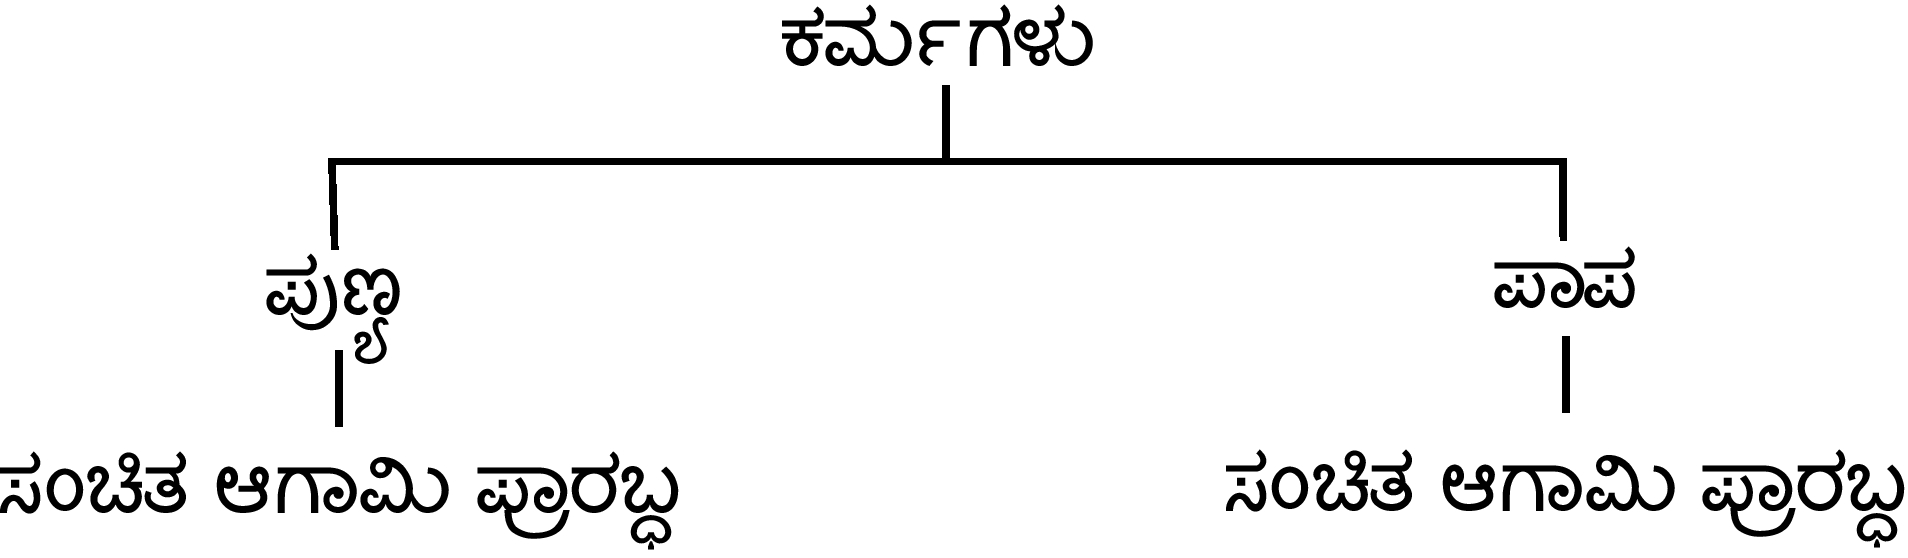
\includegraphics[scale=.95]{images/fig3.jpg}
\end{figure}


\begin{figure}[!htbp]
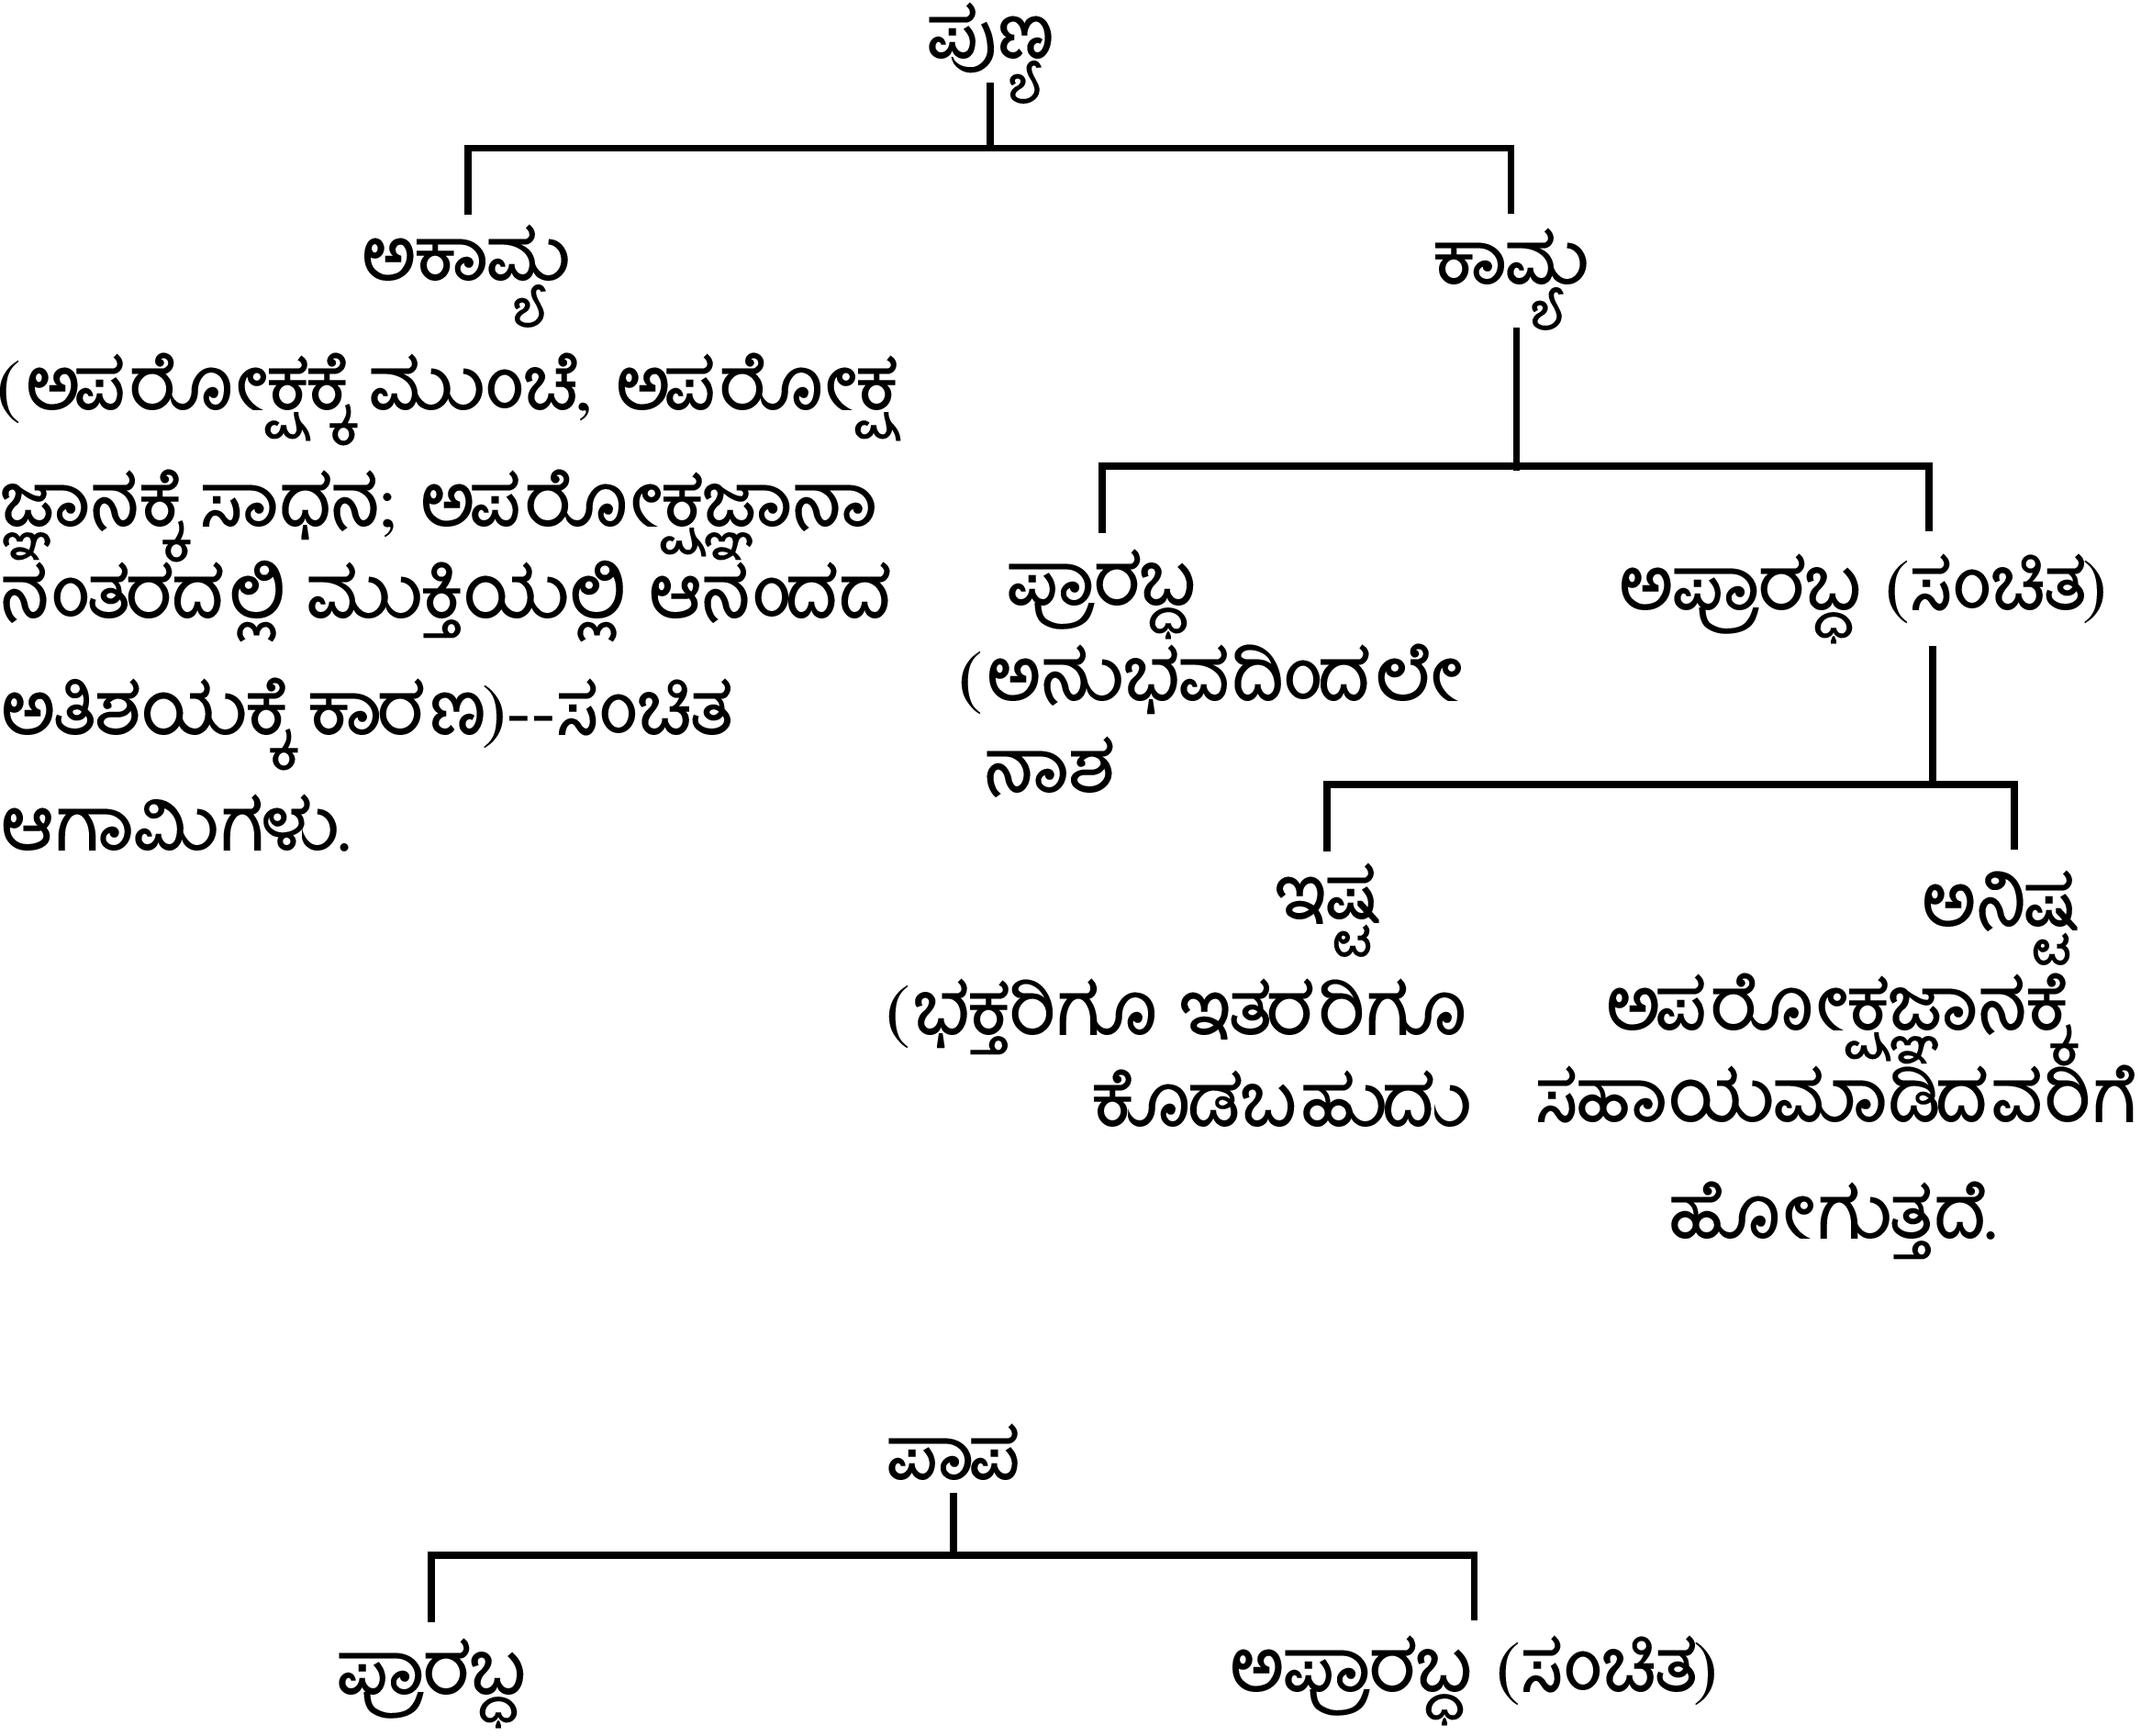
\includegraphics[scale=.95]{images/fig4.jpg}
\end{figure}

ಈ ರೀತಿಯಿಂದ ಈ ಕರ್ಮಕ್ಷಯವಾಗುವುದು ಪರಮಾತ್ಮನ ಇಚ್ಛೆಯಿಂದಲೇ ಹೊರತು ಅನ್ಯಥಾ ಅಲ್ಲ.

\textbf{(೫೯)} ನೃಣಾಂ ಸಜ್ಜನಾನಾಂ ಅರಾನ್ ದೋಷಾನ್ ಅಯತಿ ಗಮಯತಿ ಜ್ಞಾನದ್ವಾರಾ ನಾಶಯತಿ ಇತಿ ಭಗವಾನ್ ನಾರಾಯಃ-

ನೃಣಾಂ-ಸಜ್ಜನಾನಾಂ=ಸಜ್ಜನರ, ಅರಾನ್=ದೋಷಾನ್=ಪಾಪಗಳನ್ನು ಅಯತಿ=ಗಮ\-ಯತಿ=ಜ್ಞಾನದ್ವಾರಾ ನಾಶಯತಿ=ಅಪರೋಕ್ಷ ಜ್ಞಾನವನ್ನು ಕೊಟ್ಟು ನಾಶಮಾಡುತ್ತಾನೆಯಾದುದರಿಂದ, ಭಗವಾನ್= ಷಡ್ಗುಣೈಶ್ವರ್ಯಪೂರ್ಣನಾದನು, ನಾರಾಯಃ=' ನಾರಾಯ'\break ಎಂದೆನಿಸುವನು. ಣಕಾರೋ ಬಲಮಿತಿ ಶ್ರುತೇಃ ಬಲರೂಪತ್ವಾತ್ ಣಃ-'ಣ' ಎಂಬ ವರ್ಣವು, ಬಲಂ ಇತಿ=ಬಲ (ಸಾಮರ್ಥ್ಯವನ್ನು ನಿರೂಪಿಸುತ್ತದೆ ಎಂಬ ಶ್ರುತೇಃ=ಶ್ರುತಿರೀತಿಯಾಗಿ, ಬಲರೂಪತ್ವಾತ್ ಣಃ=ಬಲವನ್ನು ನಿರ್ದೇಶಿಸಲು 'ಣ' ಕಾರವನ್ನು ಉಪಯೋಗಿಸಬೇಕು. ನಾರಾಯಶ್ವಾಸೌ ಣಶ್ಚೇತಿ ನಾರಾಯಣಃ- ನಾರಾಯ ಎಂಬ ಪದಕ್ಕೆ ಬಲಸೂಚಕವಾದ ಣ ಕಾರವು ಸೇರಿ, ನಾರಾಯಣ, ನಾರಾಯನೂ ಅಗಿ 'ಣ' ನೂ ಆಗಿರುವುದರಿಂದ.

ನನ್ವೇವಂ ಸತಿ ನೃ ಅರಾಯೇತ್ಯತ್ರ ಯಣಾದೇಶೇ ನರಾಯಣೇತಿ ಸ್ಯಾದಿತಿ ಚೇತ್ ನ-

\newpage

ಏವಂ ಸತಿ=ವಿಚಾರವು ಹೀಗಿರುವಾಗ, ನೃ ಅರಾಯ ಇತ್ಯತ್ರ=ನೃ. ಅರಾಯ ಎಂದು ಸಂಧಿಕಾಲದಲ್ಲಿ, ಯಣಾದೇಶೇ=ಯಣ್ ಆದೇಶದಿಂದ ನರಾಯಣ ಇತಿ ಸ್ಯಾತ್='ನರಾಯಣ' ಎಂದು ಆಗಬೇಕು, ಇತಿ ಚೇತ್=ಹೀಗೆಂದು ಹೇಳಿದರೆ, ನ=ಅದು ಅಲ್ಲ.

(ಯಾಕೆಂದರೆ) ನೃ ಇತ್ಯತ್ರ ಋವರ್ಣಸ್ಯ ನಿರುಕ್ತೇನ ಅಕಾರ ರೂಪವರ್ಣ ವಿಕಾರಾಂಗೀಕಾರಾತ್=ನೃ ಇತ್ಯತ್ರ = ನೃ ಎಂಬಲ್ಲಿ, 'ಋ' ವರ್ಣಸ್ಯ=ಋ ಎಂಬ ವರ್ಣದ, ನಿರುಕ್ತೇನ=ರಚನೆಯ ವಿಮರ್ಶೆಯಿಂದ, ಅಕಾರರೂಪವರ್ಣ ವಿಕಾರಾಂಗೀಕಾರಾತ್='ಅ' ಎಂಬ ರೂಪ ವರ್ಣದ ವಿಕಾರಸ್ವರೂಪವೇ 'ಋ' ಕಾರ ಎಂದು ಪ್ರಾಪ್ತವಾಗುವುದರಿಂದ, (ನರಾಯಣ ಎಂದಾಗುವುದಿಲ್ಲ).

ಏವಂ ಚ ನೃ ಇತ್ಯತ್ರ ಋವರ್ಣಸ್ಯ ಅಕಾರೇ ಸತಿ ನ ಇತಿ ಜಾತೇ ನ ಅರೇತ್ಯತ್ರ ಸವರ್ಣದೀರ್ಘೇ ನಾರೇತಿ ಯುಕ್ತಮಿತ್ಯವಗಂತವ್ಯಂ-

ಏವಂ ಚ ಹೀಗಿರುವಾಗ, ನೃಇತ್ಯತ್ರ=ನೃ ಎಂಬ ವರ್ಣದಲ್ಲಿ ಅ ಕಾರೇ ಸತಿ='ಅ' ಎಂಬ ವರ್ಣವು ಇರುವಾಗ, ನ ಇತಿ ಜಾತೇ=ಇಲ್ಲ ಎಂದು ಹೇಳಬೇಕಾದ ಸಂದರ್ಭದಲ್ಲಿ, ನ ಅರೇತ್ಯತ್ರ=ನ ಅರಾಃ ಹೀಗೆ ಹೇಳುವಾಗ, ಸವರ್ಣದೀರ್ಘೇ=ಸವರ್ಣದೀರ್ಘಸಂಧಿಯಿಂದ, ನಾರಾ ಇತಿ ಯುಕ್ತಂ=ನಾರಾ ಎಂಬುವುದೇ ಸರಿ, ಇತಿ ಅವಗಂತವ್ಯಂ=ಹೀಗೆ ತಿಳಿಯಬೇಕು.

ಏವಮೇವ ಉತ್ತರತ್ರಾಪಿ ಸಮಾಧೇಯಂ-ಏವಮೇವ=ಹೀಗೆಯೇ, ಉತ್ತರತ್ರಾಪಿ=ಇನ್ನು ಮುಂದೆಯೂ ಸಹ, ಸಮಾಧೇಯಂ=ಸಮಾಧಾನ ಮಾಡಿಕೊಳ್ಳತಕ್ಕದ್ದು.

(ನೃಣಾಂ=ಸಜ್ಜನರ ಎಂಬಲ್ಲಿ, ನೃ ಎಂಬುದು ಮೂಲರೂಪ: ಈ ನೃ ಎಂಬ ವರ್ಣಕ್ಕೆ ಅರಾನ್ (ಅಯತಿ) ಎಂದು ಸಂಧಿಯಿಂದ ಸೇರಿಸಿದಾಗ, ನರಾಯ ಎಂದಾಗಬೇಕೇ ವಿನಃ ನಾರಾಯ ಎಂದಾಗುವುದಿಲ್ಲ ಎಂಬ ಅಕ್ಷೇಪಕ್ಕೆ ಉತ್ತರ ರೂಪವಾಗಿ ಹೀಗೆ ಹೇಳುತ್ತಾರೆ:-ನೃ ಎಂಬಲ್ಲಿ ನಕಾರದಮೇಲೆ ಋಕಾರವು ಇರುವುದು ಸರಿಯಷ್ಟೆ ಈ ಋಕಾರವಾದರೋ 'ಅ' ಎಂಬ ವರ್ಣದ ವಿಕಾರವೇ ಇನ್ನೊಂದು ರೂಪವೇ ಆದುದರಿಂದ ನೃ ಎಂಬಲ್ಲಿ, ನ ಮತ್ತು ಅ ಎಂದೇ ಆಗುತ್ತದೆ. ಆಗ ನ ಅರಾಃ (ದೋಷಗಳು 'ಇಲ್ಲ') ಎಂದು ಹೇಳುವಾಗ ಸವರ್ಣದೀರ್ಘ ಸಂಧಿಯಿಂದ ನಾರಾಃ ಎಂದೇ ಆಗುತ್ತದೆ, ನ+ ಅ (ನೃ ವರ್ಣದ ರೂಪಾಂತರ) + ಅರಾಃ=ನಾರಾಃ)

\begin{center}
\textbf{ಅಪರೋಕ್ಷಜ್ಞಾನದ ಮೂಲಕ ಸಜ್ಜನರ ಪಾಪ ಪರಿಹಾರ ಮಾಡುವ ಕಾರಣದಿಂದಲೂ, ಬಲರೂಪನಾದ ಕಾರಣದಿಂದಲೂ ನಾರಾಯಣ.}
\end{center}

\textbf{(೬೦)} ನೄನ್ ಅಸಜ್ಜನಾನ್ ಅರಾನ್ ದೋಷಾನ್ ಸಜ್ಜನ ದ್ರೋಹಾದಿ ರೂಪಾನ್=ನೄನ್=\-ಅಸಜ್ಜನಾನ್-ಸಜ್ಜನರಲ್ಲದವರನ್ನು, ಸಜ್ಜನ ದ್ರೋಹಾದಿ ರೂಪಾನ್=ಸತ್ಪುರುಷರಿಗೆ ದ್ರೋಹಮಾಡುವುದೇ ಮುಂತಾದ, ಅರಾನ್= ದೋಷಾನ್=ದೋಷಗಳನ್ನು; ಆ ಸಮಂತಾತ್=\-ಪೂರ್ಣವಾಗಿ; ಯಾ ಪ್ರಾಪಣ ಇತಿ ಧಾತೋ ಯಾಪಯತಿ ಪ್ರಾಪಯತಿ ಇತಿ ಭಗವಾನ್\break ನಾರಾಯಃ=ಪ್ರಾಪಣ=ತಂದೊದಗಿಸು, ಇತಿ=ಹೀಗೆಂದು ಅರ್ಥವುಳ್ಳ, ಯಾಧಾತೋಃ=ಯಾ ಎಂಬ ಧಾತುವಿನ (ಕ್ರಿಯಾಪದದ ಮೂಲ ರೂಪ) ಪ್ರಕಾರವಾಗಿ, ಯಾಪಯತಿ=ಪ್ರಾಪಯತಿ=\-ತಂದೊದಗಿಸುತ್ತಾನೆ, ಇತಿ=ಈ ಕಾರಣದಿಂದ, ಭಗವಾನ್=ಷಡ್ಗುಣೈಶ್ವರ್ಯಪೂರ್ಣನಾದ ಶ‍್ರೀಹರಿಯು, ನಾರಾಯಃ='ನಾರಾಯ' ಎಂದೆನಿಸುವನು. ಅಜಾಂ ಗ್ರಾಮಂ ಅನಯ ಇತಿವತ್ ದ್ವಿಕರ್ಮಕಃ (ಈ ಪ್ರಯೋಗದಲ್ಲಿ ಎರಡು ಕರ್ಮಪದಗಳು ನೄನ್, ಅರಾನ್-ಇರುವುದರಿಂದ ಒಂದು ಉದಾಹರಣೆಯನ್ನು ಕೊಟ್ಟು ಅದರಂತೆ ಎಂದು ಹೇಳುತ್ತಾರೆ). ಅಜಾಂ= ಆಡನ್ನು ಗ್ರಾಮಂ= ಗ್ರಾಮವನ್ನು, ಆನಯ=ಕರೆದುಕೊಂಡು ಬಾ, ಇತಿವತ್=ಇದರಂತೆ, ದ್ವಿಕರ್ಮಕಃ=ಎರಡು ಕರ್ಮಪದಗಳಿವೆ.

ಸಂಸ್ಕೃತ ಭಾಷೆಯಲ್ಲಿ ಹೀಗೆ ಎರಡು ಕರ್ಮಪದಗಳೂ ದ್ವಿತಿಯಾವಿಭಕ್ತಿಯಲ್ಲಿದ್ದರೂ, ಕನ್ನಡದಲ್ಲಿ ಅದನ್ನು ಹೇಳುವಾಗ ''ಆಡನ್ನು ಗ್ರಾಮಕ್ಕೆ (ಗ್ರಾಮವನ್ನು ಎಂದಲ್ಲ) ಕರೆದುಕೊಂಡು ಬಾ ಎಂದೇ ಹೇಳುತ್ತೇವೆ. (ಇಂಗ್ಲಿಷ್ ಭಾಷೆಯ `Tell' ಎಂಬ ಸಕರ್ಮಕ ಕ್ರಿಯಾಪದಕ್ಕೆ ಎರಡು ಕರ್ಮಪದಗಳ ಅವಶ್ಯಕತೆ ಇದ್ದಂತೆ).

"ಣಶ್ಚ ನಿರ್ವೃತಿ ವಾಚಕಃ" ಇತಿ ವಚನಾತ್ ಆನಂದರೂಪತ್ವಾತ್ ಣಃ-`ಣ' ಎಂಬ ವರ್ಣವು ಆನಂದವಾಚಕವಾದುದು ಎಂಬ ವಚನದಂತೆ ಇಲ್ಲಿ 'ಣ' ಎಂಬ ವರ್ಣವನ್ನು ಆನಂದರೂಪತ್ವಾತ್=ಆನಂದರೂಪವನ್ನು ಪಡೆದಿರುವ ಕಾರಣದಿಂದ ಎಂಬರ್ಥದಲ್ಲಿ ಉಪಯೋಗಿಸಿದರೆ, ನಾರಾಯಶ್ವಾಸೌ ಣಶ್ಚೇತಿ ನಾರಾಯಣಃ ಇತಿ ಪೂರ್ವವದ್ವಿಗ್ರಹಃ- 'ನಾರಾಯ'ನೂ ಆಗಿ, 'ಣ' ನು ಆಗಿರುವುದರಿಂದ ನಾರಾಯಣ ಎಂದಾಗುತ್ತದೆ. ಇತಿ=ಹೀಗೆಂಬ, ವಿಗ್ರಹಃ\-=ವಿಗ್ರಹವು ( ಅರ್ಥಕ್ಕೆ ಅನುಸಾರವಾಗಿ ಪದಬಿಡಿಸುವುದು), ಪೂರ್ವವತ್=ಹಿಂದಿನಂತೆಯೇ ಆಗಿದೆ-(೫೯) ರಲ್ಲಿ ಇದ್ದಂತೆ.

\begin{center}
\textbf{ ದ್ವೇಷಿಗಳಿಗೆ ಪಾಪ ಫಲವನ್ನು ಒದಗಿಸುವ ಕಾರಣದಿಂದಲೂ ಮತು ತಾನು ಆನಂದರೂಪನಾದ ಕಾರಣದಿಂದಲೂ ನಾರಾಯಣ.}
\end{center}

\noindent
\textbf{ವಿಶೇಷಾಂಶ:-}

ಅಸಜ್ಜನರಿಗೆ (ಪರಮಾತ್ಮನ ದ್ವೇಷಿಗಳಿಗೆ) ದೋಷಗಳನ್ನು ತಂದು ಒದಗಿಸುತ್ತಾನೆಂಬ ಪ್ರಮೇಯವನ್ನು ಗ್ರಹಿಸಬೇಕು.

\begin{verse}
\textbf{ಪಾಪಕರ್ಮಸಹಾಯಾ ಯೇ ಪಾಪಾತ್ಮಾನಸ್ತು ಯೇ ನರಾಃ~।}\\\textbf{ದೇವಭಾಗಗತಾತ್ಪಾಪಾತ್ತೇಭ್ಯೋಂಶಂ ದದತೇ ಹರಿಃ~।।}
\end{verse}

\vauthor{- ವಿಷ್ಣುರಹಸ್ಯ}

ಪಾಪಕರ್ಮಗಳಿಗೆ ಸಹಾಯಮಾಡುವ ಪಾಪತ್ಕರಿಗೆ (ಅಸಜ್ಜನರಿಗೆ), ತತ್ವಾಭಿಮಾನಿದೇವತೆಗಳಿಗೆ ಅವರ ಸ್ವಾತಂತ್ರ್ಯಾಂಶದಷ್ಟು ಸೇರಬೇಕಾದ ಪಾಪದಲ್ಲಿ ಒಂದಂಶವನ್ನು ಕೊಡುತ್ತಾನೆ.

ಜೀವನಿಗೆ ತಾನು ಮಾಡಿದ ಪಾಪ ಪುಣ್ಯದ ಫಲವು ಸೇರುವ ಅಂಶವು ೪೦೦ ರಲ್ಲಿ ೧೦ ಪಾಲು ಮಾತ್ರ. ಇಷ್ಟು ಅಲ್ಪಾಂಶ ಸುಖದುಃಖದಿಂದಲೇ ಮನುಷ್ಯರು ತೃಪ್ತರಾಗುತ್ತಾರೆ. ಉಳಿದ ೩೯೦ ಭಾಗವು ತತ್ವಾಭಿಮಾನಿ ದೇವತೆಗಳಿಗೂ, ತಾತ್ವಿಕದೈತ್ಯರಿಗೂ ಅವರವರ ತಾರತಮ್ಯ ಯೋಗ್ಯತೆಗೆ ಅನುಸಾರವಾಗಿ ಸೇರುತ್ತದೆ. ತತ್ವಾಭಿಮಾನಿದೇವತೆಗಳಿಗೆ ಜೀವನು ಮಾಡುವ ಪಾಪಕರ್ಮದ ಭಾಗವು ಸೇರುವುದಿಲ್ಲ. ಪಾಪಕರ್ಮದ ಅಂಶಗಳು ತಾತ್ವಿಕ ದೈತ್ಯರಿಗೂ, ಪಾಪಮಾಡಲು ಸಹಾಯಮಾಡಿದ ಇತರ ದುಷ್ಟರಿಗೂ ಸೇರುತ್ತವೆ. ಇದು ಶ‍್ರೀಹರಿಯ ಇಚ್ಛಾನುಸಾರವಾಗಿ ನಡೆಯುತ್ತದೆ.

\begin{verse}
\textbf{ಪಾಪಕರ್ಮಾಣಿ ಯೇsಪಿ ಸ್ಯುಃ ಸಹಾಯಾಃ ಪಾಪರೂಪಿಣಃ~।}\\\textbf{ಯಥಾಪರಾಧಂ ತೇಭ್ಯೋಽಪಿ ಪಾಪಾನಾಂ ವಿಭಜತ್ಯಸೌ~।।}
\end{verse}

\vauthor{-ವಿಷ್ಣುರಹಸ್ಯ}

ಪಾಪಕರ್ಮಾಚರಣೆಯಲ್ಲಿ ಯಾರು ಸಹಾಯಕರಾಗಿರುವರೋ ಅಂತಹ ಪಾಪಿಷ್ಟರಿಗೂ ಸಹ ಅವರ ಅಪರಾಧಕ್ಕೆ ಅನುಗುಣವಾಗಿ ಪಾಪಫಲವು ವಿಭಾಗಿಸಲ್ಪಡುತ್ತದೆ.

\textbf{(೬೧)} ನೄ-ಅ-ರ-ಆ ಯ ಇತ್ಯಕ್ಷರ ವಿಭಾಗಃ-'ನಾರಾಯ' ಎಂಬ ಪದದಲ್ಲಿ ನೄ + ಆ + ರ + ಆ + ಯ ಎಂಬುದಾಗಿ ಅಕ್ಷರಗಳನ್ನು ವಿಭಾಗ ಮಾಡಬಹುದು, ತತ್ರಾದ್ಯಃ ಅಜ್ ಅಭಿವಿಧ್ಯರ್ಥಕತಯಾ ಸಮಂತಾದಿತ್ಯರ್ಥಕಃ-ತತ್ರಾದ್ಯಃ ಅಜ್=ಅಲ್ಲಿ ಮೊದಲಿನ 'ಆ' ಎಂಬ ವರ್ಣವು, ಅಭಿವದ್ಯರ್ಥಕತಯಾ= ಅಭಿವ್ಯಕ್ತಿಗೊಳಿಸು ಎಂಬ ಅರ್ಥವಿರುವ ಕಾರಣದಿಂದ, ಸಮಂತಾದಿತ್ಯರ್ಥಕಃ='ಪೂರ್ಣವಾಗಿ' ಎಂಬ ಅರ್ಥವನ್ನೂ ಹೊಂದಿರುವುದು. ಅಜ್ ಮರ್ಯಾದಾಭಿವಿಧೋರಿತಿ ವಚನಾತ್-ಆ ಎಂಬ ವರ್ಣವು, ಎಲ್ಲೆಯನ್ನು ಹೆಚ್ಚುಗೊಳಿಸುವುದು ಮತ್ತು ಸಮಸ್ತವು ಎಂಬ ವಚನದಂತೆ (ಪೂರ್ಣವಾಗಿ ಎಂದು ಅರ್ಥಮಾಡಿರುವುದಕ್ಕೆ ಕಾರಣವನ್ನು ಕೊಟ್ಟಿರುತ್ತಾರೆ). ದ್ವಿತೀಯಃ ಸಮ್ಯಕ್ತ್ವಾರ್ಥಕಃ-ಎರಡನೆಯ 'ಆ' ಎಂಬ ವರ್ಣವು 'ಸರಿಯಾಗಿ', 'ಪೂರ್ಣವಾಗಿ' ಎಂಬರ್ಥವುಳ್ಳದ್ದು, ತಥಾ ಚ=ಹೀಗಿರುವುದರಿಂದ, ನೃಣಾಂ ಸಜ್ಜನಾನಾಂ ಆ ಸಮಂತಾತ್ ಸರ್ವಸ್ಟಿನ್ ಕಾಲೇ ರಂ ರಮಣಂ ಆನಂದಂ ಆ ಸಮ್ಯಕ್ ವ್ಯಕ್ತಮಿತಿ ಯಾವತ್ - 

ನೄಣಾಂ=ಸಜ್ಜನಾನಾಂ=ಸಜ್ಜನರಿಗೆ, ಆ ಸಮಂತಾತ್=ಸರ್ವಸ್ಮಿನ್ ಕಾಲೇ=ಎಲ್ಲ ಕಾಲದಲ್ಲಿಯೂ (ಪೂರ್ಣವಾಗಿ), ರಂ=ರಮಣಂ= ಆನಂದಂ=ಸುಖವು, (ಸ್ವರೂಪಸುಖವು), ಆ ಸಮ್ಯಕ್=ಒಂದೇ ಸಮನೆ (ವಿಚ್ಛತ್ತಿ ಇಲ್ಲದೆ), ವ್ಯಕ್ತಮಿತಿ ಯಾವತ್=ಅಭಿವ್ಯಕ್ತವಾಗುವುದು (ಅನುಭವಕ್ಕೆ ಬರುವುದು) ಎಂದರ್ಥ.

ಮುಕ್ತೌ ಯಾಪಯತಿ ಪ್ರಾಪಯತಿ ದದಾತಿ ಇತಿ ಯಾವದಿತಿ ಭಗವಾನ್ನಾರಾಯಃ

ಮುಕ್ತೌ=ಮುಕ್ತಿಯಲ್ಲಿ ಯಾಪಯತಿ=ಪ್ರಾಪಯತಿ=ದದಾತಿ=(ವಿಚ್ಛತ್ತಿ ಇಲ್ಲದೆ ನಿರಂತರವಾಗಿ ಪೂರ್ಣವಾದ ಸ್ವರೂಪದ ಆನಂದದ ಅನುಭವವನ್ನು) ಒದಗಿಸುವವನು, ಭಗವಾನ್=\-ಷಡ್ಗುಣೈಶ್ವರ್ಯಪೂರ್ಣನು, ನಾರಾಯಃ=ನಾರಾಯ ಎಂದೆನಿಸುವನು.

ಪೃಕ್ಷೌದರಾದಿವತ್ 'ೠ' ಕಾರಲೋಪಃ=ಈ ಉದಾಹರಣೆಯಂತೆ 'ನೃ' ಎಂಬಲ್ಲಿನ 'ೠ' ಕಾರವು ಲೋಪಹೊಂದಿತು. ಣಕಾರಾರ್ಥಶ್ಯ ಪೂರ್ವವತ್='ಣ' ಎಂಬ ವರ್ಣದ ಅರ್ಥವು ಹಿಂದಿನಂತೆಯೇ, ಅಂದರೆ ಆನಂದರೂಪೀ ಎಂದು. ಪೂರ್ವವದೇವ ವಿಗ್ರಹಃ=ವಿಗ್ರಹವೂ ಸಹ ಹಿಂದಿನ ರೀತಿಯಂತೆಯೇ.

ಅಂದರೆ, ನಾರಾಯಶ್ಚಾಸೌ ಣಶ್ಚ ನಾರಾಯಣಃ-` ನಾರಾಯ' ನೂ ಆಗಿ, 'ಣ' ನೂ ಆಗಿರುವುದರಿಂದ ನಾರಾಯಣ.

(ನಾರಾಯ ಎಂಬ ಶಬ್ದರಚನಾ ಕ್ರಮವನ್ನು ಇಲ್ಲಿ ಬೇರೊಂದು ರೀತಿಯಲ್ಲಿ ಪ್ರದರ್ಶಿಸಿ, ಣ ಎಂಬ ವರ್ಣದ ಆನಂದರೂಪೀ ಎಂಬರ್ಥವನ್ನೇ ಉಪಯೋಗಿಸಿ ನಾರಾಯಣ ಪದದ ಅರ್ಥವನ್ನು ತೋರಿಸಿರುತ್ತಾರೆ)

\begin{center}
\textbf{ಸಜ್ಜನರಿಗೆ ಮುಕ್ತಿಯಲ್ಲಿ ನಿತ್ಯಾನಂದವನ್ನು ಕೊಡುವ ಕಾರಣದಿಂದಲೂ ಮತ್ತು ತಾನು ಆನಂದಸ್ವರೂಪನಾದ ಕಾರಣದಿಂದಲೂ ನಾರಾಯಣ.}
\end{center}

\noindent
\textbf{ವಿಶೇಷಾಂಶ:-}

ಆನಂದಶ್ಯ ಮುಕ್ತಾನಾಂ ಸ ವೈ ಏಕೋ ಜನಾರ್ದನಃ ಎಂಬ ಪ್ರಮಾಣವನ್ನು ನೆನಪಿಗೆ ತಂದುಕೊಳ್ಳಬಹುದು.

\textbf{(೬೨)} ನೄಣಾಂ ಜ್ಯೋತಿಷ್ಟೋಮಾಶ್ವಮೇಧರಾಜಸೂಯಾದಿಕರ್ಮಕೃತಾಂ ಆ ಮರ್ಯಾ\-ದಯಾ ಕರ್ಮಸ್ವರೂಪತಾರತಮ್ಯೇನೇತಿ ಯಾವತ್- ನೃಣಾಂ ಜ್ಯೋತಿಷ್ಟೋಮ-ಅಶ್ವಮೇಧ-ರಾಜಸೂಯಾದಿ ಕರ್ಮಕೃತಾಂ= ಜ್ಯೋತಿಷ್ಟೋಮ, ಅಶ್ವಮೇಧ, ರಾಜಸೂಯ ಮುಂತಾದ ಕರ್ಮಗಳನ್ನು ಮಾಡಿರುವ ಸಜ್ಜನರ, ಆ=ಮರ್ಯಾದಯಾ=ಅನುಸಾರವಾಗಿ, ಕರ್ಮ\-ಸ್ವರೂಪ ತಾರತಮ್ಯೇನ=ಅವರವರ ಕರ್ಮಮಾಡಿದ ರೀತಿ ನೀತಿಗಳ ತಾರತಮ್ಯವನ್ನು ಅನುಸರಿಸಿ, ಇತಿ ಯಾವತ್=ಹೀಗೆಂಬ ಅರ್ಥದಲ್ಲಿ ರಂ=ರಮಣಂ= ಸುಖಂ=ಆನಂದವನ್ನು (ಸುಖವನ್ನು), ಆ ಲೋಕಾಪೇಕ್ಷಯಾ ಸಮ್ಯಕ್ ಸ್ವರ್ಗೇ ಯಾಪಯತೀತಿ ಭಗವಾನ್ನಾರಾಯಃ-ಆ=ಲೋಕಾಪೇಕ್ಷಯಾ= ಕರ್ಮಾನುಸಾರವಾಗಿ, ಸಮ್ಯಕ್=ಪೂರ್ತಿಯಾಗಿ, ಸ್ವರ್ಗೇ=ಸ್ವರ್ಗ\-ಲೋಕದಲ್ಲಿ ಯಾಪಯತಿ ಇತಿ=ತಂದೊದಗಿಸುತ್ತಾನೆ, ಎಂಬ ಕಾರಣದಿಂದ, ಭಗವಾನ್=\-ಷಡ್ಗುಣೈಶ್ವರ್ಯಪೂರ್ಣನಾದವನು, (ಶ‍್ರೀಹರಿಯು), ನಾರಾಯಃ= 'ನಾರಾಯ' ಎಂದು ಕರೆಯಲ್ಪಡುತ್ತಾನೆ. ಣ ಕಾರಾರ್ಥೋ ವಿಗ್ರಹಶ್ಚ ಪೂರ್ವವತ್ ದ್ರಷ್ಟವ್ಯಃ-ಣ ಎಂಬ ವರ್ಣದ ಅರ್ಥವಿವರಣೆಯನ್ನು ಹಿಂದೆ ಹೇಳಿದಂತೆ ನೋಡಿಕೊಳ್ಳತಕ್ಕದ್ದು, ಅಂದರೆ ಣ ಕಾರವು ಆನಂದರೂಪೀ ಎಂದರ್ಥ. ನಾರಾಯಣಶ್ವಾಸೌ ಣ ಶ್ವನಾರಾಯಣಃ-'ನಾರಾಯ' ನೂ ಆಗಿ ಣ ನೂ ಆಗಿರುವವನು (ಆನಂದರೂಪಿ) ನಾರಾಯಣ.

\newpage

(ಇಲ್ಲಿ 'ನಾರಾಯ' ಪದವನ್ನು ನೄ ಆ ರ ಆ ಯ ಎಂಬುದಾಗಿಯೇ ಹಿಂದಿನಂತೆ ಬಿಡಿಸಿ ಒಂದೊಂದು ವರ್ಣಕ್ಕೂ ಬೇರೆ ಅರ್ಥವಿಶೇಷವನ್ನು ಹೇಳಿರುತ್ತಾರೆ. 'ನೄ' ಎಂದರೆ ಯಜ್ಞಯಾಗಾದಿಗಳನ್ನು ಮಾಡಿರುವ ಸಜ್ಜನರೆಂದೂ, ಆ ಎಂದರೆ ಕರ್ಮಾಚರಣೆಗೆ ಅನುಗುಣವಾದ ತಾರತಮ್ಯವನ್ನು ಅನುಸರಿಸಿ ಎಂದೂ, ರ ಎಂದರೆ ರಮಣ (ಆನಂದ, ಸುಖ) ಎಂದೂ, ಆ ಎಂಬುದಕ್ಕೆ ಲೋಕಾಪೇಕ್ಷಯಾ ಪೂರ್ಣವಾಗಿ ಎಂದೂ, ಯ ಎಂದರೆ ಯಾಪಯತಿ (ಹೊಂದಿಸುತ್ತಾನೆ) ಎಂಬುದಾಗಿಯೂ ನಿರೂಪಿಸಿರುತ್ತಾರೆ. ಣ ಕ್ಕೆ ಆನಂದರೂಪೀ ಎಂದರ್ಥ. ಇಲ್ಲಿ ಸ್ವರ್ಗವೆಂಬುದನ್ನು ಉಪಲಕ್ಷಣದಿಂದ ನೋಡಬೇಕು. ಅಂದರೆ ಸ್ವರ್ಗ ಮತ್ತು ಇತರ ಸುಖಸ್ಥಾನಗಳೆಂದು ಅಭಿಪ್ರಾಯ).

\begin{center}
\textbf{ಜ್ಯೋತಿಷ್ಟೋಮವೇ ಮೊದಲಾದ ಸತ್ಕರ್ಮಮಾಡಿದವರಿಗೆ ಕರ್ಮಸ್ವರೂಪದ ತಾರತಮ್ಯಕ್ಕೆ ಅನುಗುಣವಾಗಿ ಸ್ವರ್ಗಾದಿಗಳಲ್ಲಿ ಸುಖವನ್ನು ಒದಗಿಸುವ ಕಾರಣದಿಂದಲೂ ಮತ್ತು ತಾನೇ ಆನಂದರೂಪನಾದ ಕಾರಣದಿಂದಲೂ ನಾರಾಯಣ.}
\end{center}

\textbf{(೬೩)} ನ- ಆ-ರ- ಆಯ್ ಇತ್ಯಕ್ಷರವಿಭಾಗಃ-ನ ಆ ರ ಆಯ್ ಎಂಬುದಾಗಿ ಅಕ್ಷರಗಳನ್ನು ವಿಭಾಗಿಸಬಹುದು. ತಥಾ ಚ=ಹಾಗಾದರೆ, ನ ವಿದ್ಯತೇ ಆ ಸಮಂತಾತ್ ಸರ್ವಸ್ಟಿನ್ ಅಪಿ ಕಾಲೇ ರಂ ರಮಣಂ ಸುಖಂ ಯತ್ರ ತದಂಧಂತಮೇ ನಾರಮಿತ್ಯುಚ್ಯತೇ-ಯತ್ರ=ಯಾವ ಸ್ಥಳದಲ್ಲಿ ರಂ=ರಮಣಂ=ಸುಖ=ಸುಖವು, ಆ=ಸಮಂತಾತ್=ಸರ್ವಸ್ಮಿನ್ ಕಾಲೇ ಅಪಿ= ಯಾವ ಕಾಲದಲ್ಲಿಯೇ ಆಗಲಿ, ನ ವಿದ್ಯತೇ=ಇರುವುದಿಲ್ಲವೋ, ತತ್ ಅಂಧಂ ತಮಃ=ಅಂತಹ ಅಂಧಂತಮಸ್ಸೆಂಬ ನರಕಸ್ಥಾನವು, ನಾರಂ ಇತಿ ಉಚ್ಯತೇ='ನಾರ' ಎಂದು ಹೇಳಲ್ಪಡುತ್ತದೆ.

ತತ್ ಸಮಂತಾತ್ ಸರ್ವಸ್ಮಿನ್ ಅಪಿ ಕಾಲೇ ಪುನರಾವೃತ್ತರಾಹಿತ್ಯೇನ ಕಲಾದೀನ್ ಇತಿ ಯೋಗ್ಯತಯಾ ಲಾಭಃ-ತತ್=ಅದು (ಅಂಧಂತಮಸ್ಸು), ಸಮಂತಾತ್=ಸರ್ವಸ್ಮಿನ್ ಕಾಲೇ ಅಪಿ=ಎಂದೆಂದಿಗೂ, ಪುನರಾವೃತ್ತಿ ರಾಹಿತ್ಯೇನ=ಹೊರಗೆ ಪುನಃ ಬರುವ ಅವಕಾಶವೇ ಇಲ್ಲದ ಕಾರಣದಿಂದ, ಯೋಗ್ಯತಯಾ=ಇಂತಹ ಸ್ವರೂಪ ಅರ್ಹತೆಯನ್ನುಳ್ಳ, ಕಲ್ಯಾದೀನ್ ಇತಿ= ಕಲಿಯೇ ಮೊದಲಾದ ದೈತ್ಯರನ್ನು ಎಂಬುದಾಗಿ, ಲಾಭಃ=ಫಲಿತಾರ್ಥವಾಗುತ್ತದೆ. (ಅಂದರೆ ಕಲ್ಯಾದಿ ದೈತ್ಯರು ಸದಾ ದುಃಖವನ್ನು ಅನುಭವಿಸುವ ಅಂಧಂತಮಸ್ಸೆಂಬ ನಿತ್ಯನರಕಕ್ಕೆ ನಾರ ಎಂದರ್ಥ).

ಯಾಪಯತೀತಿ ಭಗವನ್ನಾರಾಯಃ-ಆ ಕಲ್ಯಾದಿ ದೈತ್ಯರಿಗೆ ತಮಸ್ಸಿನ ವಾಸವನ್ನು ಒದಗಿ\-ಸುವ ಕಾರಣದಿಂದ, ಭಗವಾನ್ ಷಡ್ಗುಣೈಶ್ವರ್ಯಪೂರ್ಣನಾದ ಶ‍್ರೀಹರಿಯು, ನಾರಾಯಃ ನಾರಾಯ=ಣಕಾರಾರ್ಥೋ ವಿಗ್ರಹಶ್ಚ ಪೂರ್ವವದೇವಾವಗಂತವ್ಯಃ—ಣ ಕಾರದ ವಿಗ್ರಹವು (ಅರ್ಥವು) ಹಿಂದಿನಂತೆಯೇ ಎಂದು ತಿಳಿಯತಕ್ಕದ್ದು-ಅಂದರೆ ಆನಂದರೂಪೀ.

ನಾರಾಯಶ್ಚಾಸೌ ಣ ಶ್ಚ ನಾರಾಯಣಃ- `ನಾರಾಯ' ನೂ 'ಣ' ನೂ ಆಗಿರುವುದರಿಂದ ನಾರಾಯಣಃ.

\begin{center}
\textbf{ಕಲಿಯೇ ಮೊದಲಾದ ಭಗವದ್ವೇಷಿಗಳನ್ನು ನಿತ್ಯದಲ್ಲಿಯೂ ಎಂದೆಂದಿಗೂ ಮೇಲಕ್ಕೆ ಬಾರದಂತಹ ಅಂಧಂತಮಸ್ಸಿಗೆ ಹೋಗುವಂತೆ ಮಾಡುವ ಕಾರಣದಿಂದಲೂ ಮತ್ತು ಸ್ವಯಂ ಆನಂದರೂಪಿಯಾಗಿರುವ ಕಾರಣದಿಂದಲೂ ನಾರಾಯಣ.}
\end{center}

\noindent
\textbf{ವಿಶೇಷಾಂಶ:\enginline{-}}

ಭಗವದ್ವೇಷಿಗಳಾದ ಕಲಿ, ಕಾಲನೇಮಿ ಮುಂತಾದ ದೈತ್ಯರೂ, ಇತರ ತಮೋಯೋಗ್ಯ ಚೇತನರೂ, ಲಿಂಗದೇಹ ಭಂಗವಾದನಂತರ ಕಲಿಯನ್ನು ಮುಂದೆ ಮಾಡಿಕೊಂಡು ಅಂಧಂತಮ\-ಸ್ಸೆಂಬ ಮಹಾ ನರಕದಲ್ಲಿ ಬಿದ್ದು ನಿರಂತರವಾಗಿ ನಾನಾ ವಿಧವಾದ ಶಿಕ್ಷೆಯನ್ನು ಅನುಭವಿಸುತ್ತಾರೆ. ಅಲ್ಲಿಂದ ಅವರು ಎಂದಿಗೂ ಸಂಸಾರಕ್ಕೆ ವಾಪಸ್ಸು ಬರುವುದಿಲ್ಲ. ಇಂತಹ ಸ್ಥಿತಿಯು ಅವರಿಗೆ ಶ‍್ರೀಹರಿಯಿಂದಲೇ ದೊರೆಯುತ್ತದೆ

\begin{verse}
\textbf{ವಾಯೋರ್ಗದಾಪ್ರಹಾರೇಣ ತೇ ಹಿ ಕಲ್ಯಾದಯೋಽಖಿಲಾಃ~।}\\\textbf{ಭಿನ್ನಲಿಂಗಾಃ ಪತಂತ್ಯಂಧೇ ಪುನರಾವರ್ತಿವರ್ಜಿತೇ~।।}\\\textbf{ಅನಾದ್ಯನಂತೇ ವವ್ರೇಽಸ್ಮಿನ್ ಪಂಚಕಷ್ಟೇತಿದಾರುಣೇ~।}\\\textbf{ಯಥಾ ಬ್ರಹ್ಮಾ ವ್ರಜತ್ಯೇಕಃ ಪರಾಂತೇ ಮುಕ್ತಸಜ್ಜನೈಃ~।।}\\\textbf{ತಥೈವ ದುರ್ಜನೈಃ ಸಾಕಂ ಪರಾಂತೇ ಕಲಿರೇಕಲಃ~।}\\\textbf{ತಮೋಂಧಂ ಯಾತಿ ನೈಕೋಪಿ ಕದಾಪಿ ಬಹಿರಾವ್ರಜೇತ್~।।}
\end{verse}

\vauthor{-ವಿಷ್ಣುರಹಸ್ಯ}

ಕಲಿಯೇ ಮೊದಲಾದ ಸಮಸ್ತ ದೈತ್ಯರೂ ವಾಯುದೇವರ ಗದಾಪ್ರಹಾರದಿಂದ ಲಿಂಗದೇಹವನ್ನು ಪರಿತ್ಯಜಿಸಿ ಎಂದೆಂದಿಗೂ ಪುನಃ ಎದ್ದು ಬರಲಾರದ ಅಂಧಂತಮಸ್ಸಿನಲ್ಲಿ ಬೀಳುತ್ತಾರೆ. ನಿತ್ಯವಾದ ಆ ವವ್ರ ಎಂಬ ನರಕವು ಅವರ ಸ್ವರೂಪ ಇಂದ್ರಿಯಗಳಿಗೆ ದಾರುಣವಾದ ದುಃಖವನ್ನೇ ಕೊಡುವ ನರಕವು. ಪ್ರಲಯಕಾಲದಲ್ಲಿ ಮುಕ್ತಿಯೋಗ್ಯ ಸಜ್ಜನರಿಂದ ಸಹಿತರಾಗಿ ಬ್ರಹ್ಮದೇವರು ಪರಮಾತ್ಮನ ಉದರವನ್ನು ಪ್ರವೇಶಿಸುವಂತೆ, ಕಲಿಯು ಇತರ ತಮೋಯೋಗ್ಯ ಚೇತನರಿಂದ ಕೂಡಿ ಅಂಧಂತಮಸ್ಸನ್ನು ಪ್ರವೇಶಿಸುತ್ತಾನೆ. ಅಲ್ಲಿಗೆ ಹೋದವರು ಯಾರೂ ಅಲ್ಲಿಂದ ಹೊರಗೆ ಬರುವುದೇ ಇಲ್ಲ,

\begin{verse}
\textbf{ಪಾಪಂ ಪ್ರಾರಬ್ಧಪುಣ್ಯಾನಿ ತ್ವನುಭೂಯ ತತಃ ಪರಂ~।}\\\textbf{ಪತಂತಿ ಚಾಂದೇ ತಮಸಿ ದ್ವಿಷಂತ್ಯತ್ರಾಪಿ ಕೇಶವಂ~।।}\\\textbf{ಪತಿತಾನಾಂ ತಮಸ್ಯಂಧೇ ನಿಃಶೇಷಸುಖವರ್ಜಿತೇ~।}
\end{verse}

\vauthor{- ಸತ್ತತ್ವರತ್ನಮಾಲಾ}

ತಮೋಯೋಗ್ಯಚೇತನರು ಪ್ರಾರಬ್ದಪಾಪ ಮತ್ತು ಪುಣ್ಯದ ಫಲಗಳನ್ನು ಅನುಭವಿಸಿದ ನಂತರ ಅಂಧಂತಮಸ್ಸಿನಲ್ಲಿ ಬಿದ್ದು ಅಲ್ಲಿಯೂ ಪರಮಾತ್ಮನನ್ನು ದ್ವೇಷಿಸುತ್ತಾರೆ. ಅಂಧಂತಮಸ್ಸಿನಲ್ಲಿ ಬಿದ್ದವರಿಗೆ ಸುಖಲೇಶವೂ ಇರುವುದಿಲ್ಲ. ಸದಾ ದುಃಖವನ್ನೇ ಅನುಭವಿಸುತ್ತಾರೆ.

\begin{verse}
\textbf{ವಾಯೋರ್ಗದಾಪ್ರಹಾರೇಣ ತದಾ ತಲ್ಲಿಂಗಭಂಜನಂ~।}\\\textbf{ವಾಯುದೂತೈಃ ಪುರೋನೀತೋ ಯಥಾಸ್ಥಾನಂ ನಿವೇಶಿತಾಃ~।}\\\textbf{ನೈವಾಯಾತಿ ಬಹಿಸ್ತಸ್ಮಾದೇವಂ ತಾಮಸದುರ್ಗತಿಃ~।।}
\end{verse}

\vauthor{-ವಿಷ್ಣುರಹಸ್ಯ}

ವಾಯುದೇವರ ಗದಾಪ್ರಹಾರದಿಂದ ತಮೋಯೋಗ್ಯರ ಲಿಂಗದೇಹವು ಭಂಗವಾಗುತ್ತದೆ. ವಾಯುದೂತರು ಇವರನ್ನು ಅವರವರ ಯೋಗ್ಯವಾದ ತಮಸ್ಸಿನ ಸ್ಥಳಗಳಲ್ಲಿ ದಬ್ಬುತ್ತಾರೆ. ಅತ್ಯಂತ ದುಃಖವನ್ನೇ ಅನುಭವಿಸುತ್ತಾ ಅಲ್ಲಿಯೇ ಇರುವ ತಮೋಯೋಗ್ಯರು ಎಂದಿಗೂ ಮೇಲೆ ಬರುವುದೇ ಇಲ್ಲ.

\begin{verse}
\textbf{ಓಂ ಸಂಯಮನೇ ತ್ವನುಭೂಯೇತರೇಷಾಮಾರೋಹಾವರೋಹೌ ತದ್ಗತಿದರ್ಶನಾತ್ ಓಂ (೩-೧-೧೪)}
\end{verse}

ಸಂಯಮನೇ=ನರಕಗಳಲ್ಲಿ (ಪಾಪಫಲವಾದ ದುಃಖಗಳನ್ನು), ಅನುಭೂಯ ತು=ಅನು\-ಭವಿಸಿಯೇ, ಇತರೇಷಾಂ=ಇತರರಿಗೆ (ಪುಣ್ಯ ಕೆಲಸ ಮಾಡಿದವರಿಗೆ), ಆರೋಹ ಅವರೋಹೌ=ನರಕದಿಂದ ಮೇಲೆ ಬರುವುದೂ, ಮತ್ತೆ ಕೆಲವರಿಗೆ ನಿತ್ಯನರಕದಲ್ಲಿ ಬೀಳುವುದೂ ಆಗುತ್ತದೆ. ತದ್ದತಿದರ್ಶನಾತ್=ಈ ರೀತಿಯಾಗಿ ಮೇಲೆ ಬರುವುದೂ, ಕೆಳಗೆ ಬೀಳುವುದೂ ಶ್ರುತಿಯಲ್ಲಿ ಹೇಳಿರುವುದರಿಂದ.

ಸರ್ವೇ ವಾ ಏತೇಽಶುಭಕೃತಃ ಸಂಯಮನೇ ಪ್ರಪತಂತಿ ತತ್ರ ಯೇ ಪರದ್ವಿಷೋ ಗುರುದ್ವಿಷಃ ಶ್ರುತಿದ್ವಿಷಃ ತದವಮಂತಾರಃ ಶಠಾ ಮೂರ್ಖಾ ಇತಿ ತೇ ವೈ ತತೋಽವರುಹ್ಯ ತಮಸಿ ಪ್ರಪತಂತಿ ನೈವೈತ ಉತ್ತಿಷ್ಠಂತೇಪಿ ಕರ್ಹಿಚಿತ್ ವವ್ರಂ ವಾ ಏತದಿತ್ಯಾಹುರಥ ಯೇನ್ಯೇ ಬ್ರಹೃದ್ವಿಷಃ ಸ್ತೇನಾಃ ಸುರಾಪಾಃ ಇತಿ ತೇ ವೈ ತದನುಭೂಯೇಯಂ ಲೋಕಂ ಅನುವ್ರಜಂತಿ ಇತಿ ಕೌಂಠರವ್ಯ ಶ್ರುತೇಃ-

ಅಯೋಗ್ಯಕರ್ಮಮಾಡಿದವರೆಲ್ಲ ನರಕದಲ್ಲಿ ಬೀಳುತ್ತಾರೆ. ಅಲ್ಲಿ ಹರಿದ್ವೇಷಿಗಳೂ, ಗುರುದ್ವೇಷಿಗಳೂ, ವೇದನಿಂದಕರೂ, ಶಠರು, ಮುರ್ಖರು, ಎಲ್ಲ ನರಕದಿಂದ ಕೆಳಗೆ ಇಳಿದು ನಿತ್ಯನರಕದಲ್ಲಿ ಬೀಳುತ್ತಾರೆ. ಇವರು ಎಂದೂ ಏಳುವುದಿಲ್ಲ, ಅಲ್ಲಿಂದ ಅವರನ್ನು ಮೇಲಕ್ಕೆ ಎತ್ತುವವರೂ ಇಲ್ಲ. ಮತ್ತೆ ಕೆಲವರು, ಅಂದರೆ ಬ್ರಾಹ್ಮಣದ್ವೇಷಿಗಳು, ಕಳ್ಳರು, ಮದ್ಯಪಾನಮಾಡುವವರು ನರಕದುಃಖವನ್ನು ಅನುಭವಿಸಿದ ಮೇಲೆ ಭೂಲೋಕಕ್ಕೆ ಬರುತ್ತಾರೆ-ಹೀಗೆಂದು ಕೌಂಠರವ್ಯ ಶ್ರುತಿ ಹೇಳುತ್ತದೆ.

\begin{verse}
\textbf{ಓಂ ಸ್ಮರಂತಿ ಚ ಓಂ}
\end{verse}

ಸ್ಮೃತಿಗಳೂ ಸಹ ಇದೇ ವಿಷಯವನ್ನೇ ಹೇಳುತ್ತವೆ.

\begin{verse}
\textbf{ಗಚ್ಛಂತಿ ಪಾಪಿನಃ ಸರ್ವೇ ನರಕಂ ನಾತ್ರ ಸಂಶಯಃ~।}\\\textbf{ತತ್ರ ಭುಕ್ತ್ವಾ ಪತಂತ್ಯೇವ ಯೇ ದ್ವಿಷಂತಿ ಜನಾರ್ದನಂ~।।}\\\textbf{ಮಹಾತಮಸಿ ಮಗ್ತಾನಾಂ ನ ತೇಷಾಂ ಉತ್ಥತಿಃ ಕ್ವಚಿತ್~।}\\\textbf{ಇತರೇಷಾಂ ತು ಪಾಪಾನಾಂ ಉತ್ಥಾನಂ ವಿದ್ಯದೇಪಿ ಚ~।।}
\end{verse}

ಪಾಪಿಗಳೆಲ್ಲರೂ ನರಕಕ್ಕೆ ಹೋಗುವರು. ಇದರಲ್ಲಿ ಸಂದೇಹವೇ ಇಲ್ಲ. ಅಲ್ಲಿ ದುಃಖವನ್ನು ಅನುಭವಿಸಿ, ಪರಮಾತ್ಮನನ್ನು ದ್ವೇಷಿಸುವವರು ಮಹಾತಮಸ್ಸಿನಲ್ಲಿ ಬೀಳುವರು. ಅಲ್ಲಿಂದ ಅಂತಹವರಿಗೆ ಮೇಲೆ ಬರೋಣವೆಂಬುದೇ ಇಲ್ಲ. ಇತರರಿಗೆ (ಹರಿದ್ವೇಷವಲ್ಲದ ಇತರ ಪಾಪಕರ್ಮ ಮಾಡಿದವರಿಗೆ) ಮೇಲೆ ಬರೋಣವು ಇರುತ್ತದೆ.

\begin{verse}
\textbf{ಕೇವಲೇನ ಹ್ಯಧರ್ಮೇಣ ಕುಟುಂಬ ಭರಣೋತ್ತುಕಃ~।}\\\textbf{ಯಾತಿ ಜೀವೋಂಧತಾಮಿಸ್ರಂ ಚರಮಃ ತಮಸಃ ಪದಂ~।।}
\end{verse}

\vauthor{-ಭಾಗವತ}

ಅಸುರ ಸ್ವಭಾವವುಳ್ಳ ಜೀವನು ಕುಟುಂಬ ರಕ್ಷಣೆಯಲ್ಲಿಯೇ ಸದಾ ಆಸಕ್ತನಾಗಿ ಶ‍್ರೀಹರಿಯ ದ್ವೇಷ ಹರಿಭಕ್ತರ ದ್ವೇಷ ಮುಂತಾದ ಅಧರ್ಮ ಕರ್ಮಗಳಿಂದ ಅಂತಿಮವಾದ ಅಂಧಂತಮಸ್ಸೆಂಬ ಅಜ್ಞಾನ ಅಂಧಕಾರಗಳಿಗೆ ಮುಖ್ಯಾಶ್ರಯವಾದ ಸ್ಥಾನವನ್ನು ಹೊಂದುತ್ತಾನೆ. ಇದು ಶ್ರುತಿ ಪ್ರಸಿದ್ಧವು.

ಹರಿಗುರು ದ್ವೇಷಿಗಳಿಗೆ ಆಗುವ ನರಕದುಃಖವನ್ನು ವಾಯುಸ್ತುತಿಯಲ್ಲಿಯೂ ವರ್ಣಿಸಲಾಗಿದೆ.

ಹರಿದ್ವೇಷವೆಂದರೆ ಪರಮಾತ್ಮನನ್ನು ಮಾತ್ರ ದ್ವೇಷ ಮಾಡುವುದು ಎಂದಲ್ಲ. ಹೇಗೆ ಪರಮಾತ್ಮನ ಭಕ್ತಿಯಲ್ಲಿ ಒಂಭತ್ತು ಬಗೆ ಇದೆಯೋ, ದ್ವೇಷದಲ್ಲಿಯೂ ಸಹ ಒಂಭತ್ತು ರೀತಿ ಇದೆ:-

\begin{verse}
\textbf{ಜೀವಾಭೇದೋ ನಿರ್ಗುಣತ್ವಂ ಅಪೂರ್ಣಗುಣತಾ ತಥಾ~।}\\\textbf{ಸಾಮ್ಯಾಧಿಕ್ಕೇ ತದನ್ಯೇಷಾಂ ಭೇದಃ ತದ್ಧತ ಏವ ಚ~।।}\\\textbf{ಪ್ರಾದುರ್ಭಾವವಿಪರ್ಯಾಸಃ ತದ್ಭಕ್ತದ್ವೇಷ ಏವ ಚ~।}\\\textbf{ತತ್ಪ್ರಮಾಣಸ್ಯ ನಿಂದಾ ಚ ದ್ವೇಷಾ ಏತೇsಖಿಲಾ ಮತಾಃ~।।}
\end{verse}

\vauthor{-ನಿರ್ಣಯ}

ಜೀವನೂ ಶ‍್ರೀಹರಿಯೂ ಒಂದೇ ಎಂದು ತಿಳಿಯುವುದು, ಶ‍್ರೀಹರಿಗೆ ಯಾವ ಗುಣವೂ ಧರ್ಮವೂ ಇಲ್ಲವೆನ್ನುವುದು, ಗುಣವಿದ್ದರೂ ಅಪೂರ್ಣನೆಂದು ಹೇಳುವುದು, ಇತರ ದೇವತೆಗಳು ಶ‍್ರೀಹರಿಗೆ ಸಮರೆಂದೋ ಅಧಿಕರೆಂದೂ ಹೇಳುವುದು, ಶ‍್ರೀಹರಿಯ ಅವಯವಗಳಲ್ಲಿ ಅವತಾರಗಳಲ್ಲಿ, ಅವತಾರೂಪಗಳಿಗೂ ಮೂಲರೂಪಕ್ಕೂ ಭೇದ ಇದೆ ಎಂದು ತಿಳಿಯುವುದು, ಅವತಾರರೂಪಗಳನ್ನು ಸಾಮಾನ್ಯ ಮಾನವನಂತೆ ಎಂದು ಹೇಳುವುದು, ಹರಿಭಕ್ತರನ್ನು ದ್ವೇಷಿಸುವುದು, ಹರಿಯನ್ನು ಪ್ರತಿಪಾದಿಸುವ ವೇದಗಳನ್ನು (ತದನುಸಾರಿಯಾದ ಇತರ ಶಾಸ್ತ್ರ ಗ್ರಂಥಗಳನ್ನೂ) ಅಪ್ರಮಾಣವೆಂದು ನಿಂದಿಸುವುದು-ಇವೆಲ್ಲ ವಿಷ್ಣುವನ್ನು ದ್ವೇಷಮಾಡಿದಂತೆಯೇ. ಹೀಗೆ ಮಾಡುವವರಿಗೆ ಮೇಲೆ ಹೇಳಿದ ಪ್ರಮಾಣಗಳಲ್ಲಿರುವಂತೆ ಅಂಧಂತಮಸ್ಸೇ ಗತಿ.

\textbf{(೬೪)} ನ-ಆ-ಅರ-ಆಯ ಇತಿ ಪದವಿಭಾಗಃ-`ನಾರಾಯ' ಎಂಬ ಪದದಲ್ಲಿರುವ ವರ್ಣಗಳನ್ನು ನ-ಆ-ಅರ-ಆಯ ಹೀಗೆ ವಿಭಜಿಸ ಬಹುದು. `ಅಮಾನೋನಾಃ ಪ್ರತಿಷೇಧೇ' ಇತಿ ಸ್ಮರಣಾತ್ ದೈತ್ಯಾನಾಂ ಸುಖಪ್ರತಿಷೇಧ ಕರ್ತೃತ್ವಾತ್ ನಃ- `ಅಮಾನೋನಾಃ ಪ್ರತಿಷೇಧೇ' ಇತಿ ಸ್ಮರಣಾತ್-ಅಮ, ನೋ, ನ ಈ ಪ್ರತ್ಯಯಗಳು `ಇಲ್ಲ, ಅಲ್ಲ ಬೇಡ' ಎಂಬ ಅರ್ಥ ಉಳ್ಳವುಗಳು ಎಂಬುದಾಗಿ ನೆನಸಿದರೆ, ದೈತ್ಯಾನಾಂ=ದೈತ್ಯರಿಗೆ, ಸುಖಪ್ರತಿಷೇಧಕರ್ತೃತ್ವಾತ್=ಸುಖ ಉಂಟಾಗದಂತೆ ತಡೆಮಾಡುವ ಕಾರಣದಿಂದ, ನಃ='ನ' ಎಂಬ ವರ್ಣವು ಪ್ರಯೋಗಿಸಲ್ಪಟ್ಟಿದೆ. ಪ್ರತಿಷೇಧೋ ಜಗದಭಾವಃ ಪ್ರಲಯಃ ಇತಿ ಯಾವತ್-ಪ್ರತಿಷೇಧಃ= ತಡೆಮಾಡುವುದು, ಜಗದಭಾವಃ=ಪ್ರಲಯಃ=ಜಗತ್ತು ಇಲ್ಲದಿರುವುದು ಅಂದರೆ ಪ್ರಳಯಕಾಲ, ಇತಿ, ಯಾವತ್=ಹೀಗೆಂದು ಹೇಳಬಹುದು. ತತ್ಕರ್ತೃತ್ವಾದ್ವಾ ನಃ- ಆ ಪ್ರಳಯಕಾರಕನೂ ಆಗಿರುವುದರಿಂದಲೂ 'ನ' ಎಂದು ಹೇಳಬಹುದು. ಋ ಗತೌ-ಋ ಎಂಬ ವರ್ಣವು ಗತಿಯನ್ನು ಸೂಚಿಸುವಂತಹುದು. ಅಸ್ಸಾತ್ ಕರ್ಮಣಿ ಆಕಾರ ಪ್ರತ್ಯಯೇ ಗುಣೇ ಚ ಸತಿ ಅರೇತಿ ರವತಿ-(ಈ 'ಋ' ಕಾರವು 'ಅ' ಕಾರದ ಇನ್ನೊಂದು ರೂಪವಾದುದರಿಂದ) ಋ ಕಾರಕ್ಕೆ 'ಅ' ಕಾರವನ್ನು ಕರ್ಮಣಿ ಪ್ರಯೋಗದಲ್ಲಿ ಸೇರಿಸಿ ದೀರ್ಘಮಾಡಿದಾಗ `ಅರಾ' ಎಂದಾಗುತ್ತದೆ. ತಥಾ ಚ=ಹಾಗೆಯೇ, ಆ ಸಮ್ಯಕ್ ಬ್ರಹ್ಮಾದಿಭಿಃ ಜ್ಞೇಯತ್ವಾತ್ ಆ ಅರೇತ್ಯುಚ್ಯತೇ-ಆ= ಸಮ್ಯಕ್=ಸಮಸ್ತರಾದ, ಬ್ರಹ್ಮಾದಿಭಿಃ=ಬ್ರಹ್ಮದೇವರೇ ಮುಂತಾದವರಿಂದ, ಜ್ಞೇಯತ್ವಾತ್=ಯಥಾ ಯೋಗ್ಯವಾಗಿ ತಿಳಿಯಲ್ಪಡುತ್ತಾನೆಯಾದುದರಿಂದ, `ಆ=ಅರಾ' ಎಂದು ಹೇಳಲಾಗುತ್ತದೆ. ಯಾ ಪ್ರಾಪಣೆ ಇತಿ ಧಾತೋಃ-'ಯಾ' ಎಂದರೆ ಹೊಂದಿಸುವುದು ಎಂದರ್ಥ ಉಳ್ಳ ಧಾತುವಿನ, ಪ್ರಾಪಣಾರ್ಥಾನಾಂ ಗತ್ಯರ್ಥತ್ವಾತ್=(ಪರಮಾತ್ಮನನ್ನು) ಹೊಂದಬೇಕೆಂಬ ಇಚ್ಛೆಯುಳ್ಳವರಿಗೆ ಗತಿಪ್ರದನಾಗಿರುವುದರಿಂದ, ಗತ್ಯರ್ಥಾನಾಂ ಚ ಅವಗತ್ಯರ್ಥತ್ವಾತ್=ಗತಿಯನ್ನು ಅಪೇಕ್ಷಿಸುವವರಿಗೆ (ತನ್ನ ವಿಷಯಕವಾದ) ಜ್ಞಾನವನ್ನು ಪಡೆದಿರಬೇಕೆಂದು ಇರುವುದರಿಂದಲೂ, ಆ ಸಮ್ಯಕ್ ಸ್ವಪರಗತಾಶೇಷವಿಶೇಷವಿಷಯಕೇತಿ ಯಾವತ್-ಅ=ಸಮ್ಯಕ್=ಪೂರ್ತಿಯಾದ, ಸ್ವಪರಗತ=ತನ್ನ ಮತ್ತು ಇತರರ ಸಂಬಂಧಪಟ್ಟ ಅಶೇಷ ವಿಶೇಷ=ಸಮಸ್ತವಾದ ಹಾಗೂ ಅಸಾಧಾರಣವಾದ, ವಿಷಯಕ ಇತಿ ಯಾವತ್=ವಿಷಯಸಂಬಂಧವಾದುದು ಎಂದರ್ಥ. ಯಂ ಜ್ಞಾನಂ ಯಸ್ಕಾಸೌ ಅಯಃ- ಯಸ್ಯ=ಯಾರಿಗೆ, ಯಂ=ಜ್ಞಾನಂ=ಜ್ಞಾನವು ಇದೆಯೋ, ಅಸೌ= ಅಂತಹವನು, ಆಯಃ=\-'ಆಯ' ಎಂದು ಹೇಳಲ್ಪಡುತ್ತಾನೆ. ಬಲಾನಂದ ರೂಪತ್ವಾತ್ ಣಃ=ಬಲ, ಆನಂದ ಇವುಗಳ ರೂಪವಾಗಿರುವುದರಿಂದ 'ಣ' ಎಂದು ಹೇಳಲ್ಪಡುತ್ತಾನೆ. ತಥಾ ಚ ನಶ್ಯಾಸೌ ಆ ಅರಶ್ಚಾಸೌ ಆಯಶ್ಚಾಸೌ ಣ ಶ್ಚೇತಿ, ಅಂದರೆ 'ನ' ಆಗಿ, 'ಆ' ಆಗಿ, 'ಅರ' ನು ಆಗಿ, 'ಆಯ' ನು ಆಗಿ, 'ಣ' ನು ಆಗಿರುವವನು, ಭಗವಾನ್ನಾರಾಯಣಃ-ಷಡ್ಗುಣೈಶ್ವರ್ಯಪೂರ್ಣನಾದ ನಾರಾಯಣ.

ಈ ಪ್ರಕರಣದಲ್ಲಿ `ನಾರಾಯಣ' ಶಬ್ದವನ್ನು ವಿಭಜಿಸಿ ಒಂದೊಂದು ವರ್ಣಕ್ಕೂ ಬೇರೆ ಬೇರೆ ಕೃತ್ಯಗಳನ್ನು ಹೇಳಿರುತ್ತಾರೆ.

'ನಾರಾಯಣ' ಶಬ್ದವು ಹೀಗೆ ವಿಭಜಿಸಲಾಗಿದೆ:-

ನ-ಆ-ಅರ-ಆಯ-ಣ.

\begin{itemize}
\item ನ=ಇಲ್ಲ, ಅಲ್ಲ, ಬೇಡ ಎಂಬ ಅರ್ಥ ಉಳ್ಳದ್ದು, ದೈತ್ಯರಿಗೆ ಸುಖಬಾರದಂತೆ ಮಾಡುವುದು, ಪ್ರಳಯದಲ್ಲಿ ಜಗತ್ತು ಇಲ್ಲದಂತೆ ಮಾಡುವುದು-ಈ ಅರ್ಥದಲ್ಲಿ 'ನ' ಉಪಯೋಗಿಸಲಾಗಿದೆ.

 \item ಆ=ಸಮಸ್ತವಾದ, ಬ್ರಹ್ಮದೇವರೇ ಮೊದಲಾದ ಎಲ್ಲರಿಂದ ಎಂದರ್ಥ.

 \item ಅರ=ಋಕಾರವು ಗತಿ ಎಂಬ ಅರ್ಥ ಉಳ್ಳದ್ದು, ಈ ಋಕಾರಕ್ಕೆ ಅಕಾರ ಪ್ರತ್ಯಯನ್ನು ಸೇರಿಸಿದರೆ 'ಅರ' ಎಂದಾಗುತ್ತದೆ. ಬ್ರಹ್ಮದೇವರೇ ಮೊದಲಾದ ಸಮಸ್ತರಿಂದ ಯಥಾಯೋಗ್ಯವಾಗಿ ತಿಳಿಯಲ್ಪಡತಕ್ಕವನು ಎಂಬರ್ಥದಲ್ಲಿ ಅರ ಎಂದು ಹೇಳಲಾಗುತ್ತದೆ.

 \item ಆಯ್=ಯಾ ಎಂಬ ಧಾತುವಿಗೆ ಪ್ರಾಪಣ (ಹೊಂದಿಸುವುದು) ಎಂದರ್ಥ, ಪ್ರಾಪಣಾರ್ಥ ಧಾತು ಗತ್ಯರ್ಥ (ಗತಿಯೇ ಎಂಬ ಅರ್ಥ) ಉಳ್ಳದ್ದು. ಗತ್ಯರ್ಥವುಳ್ಳವುಗಳಿಗೆ ಅವಗತಿ (ಜ್ಞಾನ, ತಿಳಿಯುವುದು) ಎಂದರ್ಥ. ಅಂದರೆ ಪರಮಾತ್ಮನು ತನ್ನ ಬಗ್ಗೆ, ಮತ್ತು ಇತರ ಸಮಸ್ತ ವಸ್ತುಗಳ ಬಗ್ಗೆ ಅಸಾಧಾರಣ ಸಂಪೂರ್ಣಜ್ಞಾನ ಉಳ್ಳವನು ಎಂದು ತಾತ್ಪರ್ಯ, ಜ್ಞಾನಕ್ಕೆ ಆಶ್ರಯನು ಎಂದು ತಿಳಿಯಬೇಕು.

 \item ಣ=ಬಲ, ಆನಂದ ಇವೇ ರೂಪವಾಗಿ ಇರುವವನು.

\end{itemize}

ಈ ಕೃತ್ಯಗಳಿಂದ ''ನ-ಆ-ಅರ-ಆಯ್-ಣ'' ಉಪಯೋಗಿಸಲ್ಪಟ್ಟು ನಾರಾಯಣ ಎಂಬ ಪದವಾಗಿ ವಿಶೇಷ ಅರ್ಥ ದ್ಯೋತಕವಾಗಿದೆ. ದ್ವೇಷಿಗಳಿಗೆ ಸುಖಪ್ರಾಪ್ತವಾಗದಂತೆ ಮಾಡುವ, ಜಗತ್ತಿಗೆ ಪ್ರಳಯಕಾರಕನು ಆಗುವ, ಬ್ರಹ್ಮಾದಿಗಳಿಂದ ಯಥಾವತಿ ತಿಳಿಯಲ್ಪಡುವ, ತನ್ನ ವಿಷಯಕವಾದ ಮತ್ತು ಇತರ ಸಮಸ್ತ ವಸ್ತುವಿಷಯಕವಾದ ಅಸಾಧಾರಣ ಸಂಪೂರ್ಣ ಜ್ಞಾನವನ್ನು ಹೊಂದಿರುವ, ಬಲ- ಆನಂದ ಇವುಗಳೇ ರೂಪವಾಗಿ ಉಳ್ಳ ಕಾರಣಗಳಿಂದ ನಾರಾಯಣ.

\textbf{(೬೫)} ನ ವಿದ್ಯಂತೇ ಅರಾಃ ದೋಷಾಃ ಯಸ್ಯೇತಿ ನಾರಃ- ಯಸ್ಯ= ಯಾರಿಗೆ, ಅರಾಃ=ದೋಷಾಃ=ದೋಷಗಳು, ನ ವಿದ್ಯಂತೇ=ಇಲ್ಲವೋ, ಇತಿ=ಹೀಗಿರುವುದು, ನಾರಃ=\-'ನಾರ' ಎಂದೆನಿಸುವನು-ಅಂದರೆ ದೋಷ ರಹಿತನೆಂದರ್ಥ. ಸರ್ವಾಧಿಕತ್ವಾತ್ ಅಃ=\break ಎಲ್ಲಕ್ಕಿಂತಲೂ ಶ್ರೇಷ್ಠತೆಯನ್ನು ಹೇಳುವುದರಿಂದ 'ಅ' ಎಂಬ ವರ್ಣವು ಸೇರುತ್ತದೆ. ಅಕಾರಸ್ಕಾಧಿಕಾರ್ಥತಃ ಇತ್ಯುಕೇಃ='ಅ'ಕಾರಕ್ಕೆ "ಎಲ್ಲಕ್ಕಿಂತಲೂ ಶ್ರೇಷ್ಠ" ಎಂದಿರುವುದರಿಂದ ಮೇಲೆ ಹೇಳಿದಂತೆ ಅ ಕಾರವನ್ನು ಸೇರಿಸಬೇಕು. ಜ್ಞಾನರೂಪತ್ವಾತ್ ಮುಕ್ತ ಪ್ರಾಪ್ಯತ್ವಾತ್ ವಾ ಅಯಃ- `ಅಯಃ' ಎಂಬ ಪದವು ಜ್ಞಾನರೂಪಿಯಾಗಿರುವುದರಿಂದ ಅಥವಾ ಮುಕ್ತರಿಂದ ಹೊಂದಲ್ಪಡುವವನಾದುದರಿಂದ (ಸೇರುತ್ತದೆ). ಅಂದರೆ `ಅಯಃ' ಎಂಬ ಪದಕ್ಕೆ ಜ್ಞಾನರೂಪಿ ಅಥವಾ ಮುಕ್ತಪ್ರಾಪಕ ಎಂದರ್ಥ. ಯಥೋಕ್ತಂ ಬೃಹದ್ಭಾಷ್ಯೇ-' ಬೃಹದ್ಭಾಷ್ಯ' ದಲ್ಲಿ ಹೀಗೆ ಹೇಳ\-ಲಾಗಿದೆ-ಜ್ಞಾನರೂಪತ್ವತೋ ವಾಽಯಃ ಮುಕ್ತ ಪ್ರಾಪ್ಯತ್ವತೋಽಥವೇತಿ-ಜ್ಞಾನವೇ ಶರೀರವಾಗಿ ಉಳ್ಳವನಾದ ಕಾರಣದಿಂದ ಅಥವಾ ಮುಕ್ತರಿಂದ ಹೊಂದಲ್ಪಡುವ ಕಾರಣದಿಂದ, 'ಅಯಃ' ಎಂಬ ಪದವು ಪ್ರಯೋಗಿಸಲ್ಪಡುತ್ತದೆ. ಬಲಾನಂದರೂಪತ್ವಾತ್ ಣಃ- ಬಲ, ಆನಂದ ಇವುಗಳೇ ರೂಪವಾಗಿ ಉಳ್ಳವನು ಎಂದು ಹೇಳಲು 'ಣ' ಕಾರವು ಪ್ರಯೋಗಿಸಲ್ಪಡುತ್ತದೆ. ತಥಾಚ, ನಾರಶ್ಚಾಸ್‌ ಅಶ್ವಾಸೌ ಯಶ್ವಾಸೌ ಣಶ್ಚೇತಿ ಭಗವಾನ್ನಾರಾಯಣಃ-ಹೀಗೆ, 'ನಾರ' ನಾಗಿರುವುದರಿಂದಲೂ (ದೋಷರಹಿತನಾದುದರಿಂದ), 'ಅ' ಆಗಿರುವುದರಿಂದ (ಸರ್ವರಿಂದಲೂ ಶ್ರೇಷ್ಠನಾಗಿರುವುದರಿಂದ), 'ಅಯ' ಆಗಿರುವುದರಿಂದ ಜ್ಞಾನರೂಪಿಯೂ ಮುಕ್ತಪ್ರಾಪ್ಯನೂ ಆಗಿರುವುದರಿಂದ), 'ಣ' ಆಗಿರುವುದರಿಂದ (ಬಲ ಮತ್ತು ಆನಂದವೇ ಶರೀರವಾಗಿ ಉಳ್ಳವನು)-ಈ ಕಾರಣಗಳಿಂದ ನಾರಾಯಣ.

(ಇಲ್ಲಿ ನಾರ, ಅ, ಅಯ, ಣ ಎಂದು ವಿಭಜಿಸಿ ಒಂದಕ್ಕೊಂದು ಅರ್ಥವನ್ನು ನಿರೂಪಿಸಿರುತ್ತಾರೆ).

\begin{center}
\textbf{ದೋಷರಹಿತನಾದುದರಿಂದ, ಸರ್ವಶ್ರೇಷ್ಠನಾದುದರಿಂದ ಜ್ಞಾನರೂಪನಾದುದರಿಂದ, ಮುಕ್ತರಿಂದ ಪ್ರಾಪ್ಯನಾದುದರಿಂದ, ಬಲ-ಆನಂದ ಇವುಗಳೇ ಶರೀರವಾಗಿ ಉಳ್ಳ ಕಾರಣದಿಂದ ನಾರಾಯಣ.}
\end{center}

\textbf{(೬೬)} ಉಕ್ತರೀತ್ಯಾ ನಿರ್ದೋಷತ್ವಾತ್ ಭಗವಾನ್ ನಾರಃ-ಉಕ್ತರೀತ್ಯಾ=ಆಗಲೇ ಹೇಳಿದ ರೀತಿಯಲ್ಲಿ ನಿರ್ದೋಷತ್ವಾತ್=ದೋಷ ವರ್ಜಿತನಾದುದರಿಂದ, ಭಗವಾನ್=ಪರಮಾತ್ತನು, ನಾರಃ='ನಾರ' ಎಂದೆನಿಸುವನು. ಆಯಾನ್ ಸಮ್ಯಕ್ ಜ್ಞಾನರೂಪಾನ್ ನರಾನ್ ಸ್ವಸಮೀಪಂ ಆನಯತಿ ಸಮ್ಯಗಾನಂದವ್ಯಕ್ತ್ಯಾದಿಕಂ ದತ್ವಾ ನಯತಿ ಇತಿ ವಾ ಭಗವಾನ್ ಆಯನಃ-ಆಯಾನ್=ಸಮಸ್ತ, ಸಮ್ಯಕ್ ಜ್ಞಾನರೂಪಾನ್=ಯಥಾರ್ಥ ಜ್ಞಾನರೂಪ ಉಳ್ಳ, ನರಾನ್=ಸಜ್ಜನರನ್ನು ಸ್ವಸಮೀಪಂ=ತನ್ನ ಬಳಿಗೆ, ಆನಯತಿ=ಕರೆಸಿಕೊಳ್ಳುತ್ತಾನೆ. ವಾ=ಅಥವಾ, ಸಮ್ಯಗ್=\break ನಿರ್ದುಃಖವಾದ, ಆನಂದ ವ್ಯಕ್ತ್ಯಾದಿಕಂ=ಸ್ವರೂಪಭೂತ ಆನಂದದ ಅನುಭವವೇ ಮೊದಲಾದು\-ದನ್ನು, ದತ್ತಾ=ಕೊಟ್ಟು, ನಯತಿ=ಕರೆದುಕೊಂಡು ಹೋಗುತ್ತಾನೆ, ಇತಿ=ಹೀಗಿರುವುದರಿಂದ, ಭಗವಾನ್=ಷಡ್ಗುಣೈಶ್ವರ್ಯಪೂರ್ಣನಾದವನು, ಆಯನಃ=' ಆಯನ' ಎಂದೆನಿಸುವನು. ನಾರಾಶ್ಚಾಸೌ ಆಯನಶ್ಚೇತಿ ನಾರಾಯಣಃ-'ನಾರ' ನೂ ಆಗಿ, 'ಆಯನ' ನೂ ಆಗಿರುವುದರಿಂದ, ನಾರಾಯಣ. (ನಾರಾಯನ ಎಂದಾಗುವುದಿಲ್ಲ, ರಷಾಭ್ಯಾಂ ನೋಣಃ ಸಮಾನಪದೇ ಎಂಬ ಸೂತ್ರದ ಪ್ರಕಾರ ನಾರಾಯಣ ಎಂದಾಗುತ್ತದೆ).

\begin{center}
\textbf{ನಿರ್ದೋಷನಾದ ಕಾರಣದಿಂದಲೂ, ಅಪರೋಕ್ಷಜ್ಞಾನಯುಕ್ತರಾದವರನ್ನು ತನ್ನ ಸಮೀಪಕ್ಕೆ ಕರೆದುಕೊಳ್ಳುವ ಕಾರಣದಿಂದಲೂ ನಾರಾಯಣ.}
\end{center}

\textbf{(೬೭)} ಅರ ಶಬ್ದೋ ಅರ್ಶಾದ್ಯಜಂತಃ-'ಅರ' ಶಬ್ದವು ಅಜಂತವೆಂಬ ಶಬ್ದದ ಗುಂಪಿಗೆ ಸೇರಿದುದು. ತಥಾ ಚ=ಹೀಗಿರುವುದರಿಂದ, ಅರೈಃ ದೋಷವದ್ಭಿಃ ಅಯತೇ ಗಮ್ಯತೇ ಇತ್ಯರಾಯಃ-ಅರೈಃ=ದೋಷವದ್ಭಿಃ=ದೋಷ ಉಳ್ಳವರಿಂದ (ಪಾಪ ಮಾಡಿದವರಿಂದ), ಅಯತೆ=ಗಮ್ಯತೇ=ಹೊಂದಲ್ಪಡುತ್ತಾನೆ, ಇತಿ ಅರಾಯಃ=ಹೀಗಿರುವುದರಿಂದ ಅರಾಯ ಎಂದಾಗು\-ತ್ತದೆ. ಅಂದರೆ ಪಾಪ ಮಾಡಿದವರೂ ಅವನನ್ನು ಹೊಂದಬಹುದಾಗಿದ್ದರೆ ಅರಾಯ. ನ ಅರಾಯಃ ನಾರಾಯಃ ಇತಿ-ನ ಅರಾಯಃ-ಅರಾಯನು ಅಲ್ಲದಿರುವುದರಿಂದ ನಾರಾಯ. (ಪಾಪಮಾಡಿದವರು ಅವನ ಬಳಿ ಹೋಗಲು ಸಾಧ್ಯವಿಲ್ಲವೆಂದರ್ಥ). ಉಕರೀತ್ಯಾ ನಾರೈಃ ನಿರ್ದೋಷೈಃ ನರೈಃ ಅಯತೇ ಗಮ್ಯತೇ ಇತಿ ನಾರಾಯಃ-ಅಥವ, ಉಕ್ತರೀತ್ಯಾ-ಆಗಲೇ ಹೇಳಿದಂತೆ, ನಾರೈಃ=ನಿರ್ದೋಷೈಃ ನರೈಃ =ದೋಷರಹಿತರಾದ ಸಜ್ಜನರಿಂದ, ಅಯತೆ=ಗಮ್ಯತೇ=\-ಹೊಂದಲ್ಪಡತಕ್ಕವನು, ಇತಿ ನಾರಾಯಃ=ಹೀಗಿರುವುದರಿಂದ ನಾರಾಯ. (ದೋಷರಹಿತರಾದವರು ಅಂದರೆ ಪಾಪಗಳನ್ನು ಕಳೆದುಕೊಂಡವರು ಅವನನ್ನು ಹೊಂದಬಹುದೆಂದು ತಾತ್ಪರ್ಯ). ಣ ಕಾರಾರ್ಥಸ್ತು ಉಕ್ಕ ಏವ='ಣ' ಎಂಬ ವರ್ಣದ ಅರ್ಥವು ಆಗಲೇ ಹೇಳಲ್ಪಟ್ಟಿದೆ (ಆನಂದ- ಬಲ- ರೂಪೀ ಎಂದು). ತಥಾ ಚ ನಾರಾಯಶ್ಚಾಸೌ ಣ ಶ್ವೇತಿ ಭಗವನ್ನಾರಾಯಣಃ-ಹೀಗಿರುವುದರಿಂದ, 'ನಾರಾಯ' ನೂ ಆಗಿ, 'ಣ' ನೂ ಆಗಿರುವವನು ಷಡ್ಗುಣೈಶ್ವರ್ಯಪೂರ್ಣನಾದ ನಾರಾಯಣ

\begin{center}
\textbf{ದ್ವೇಷಿಗಳಿಂದ ಹೊಂದಲ್ಪಡತಕ್ಕವನಲ್ಲವಾದ ಕಾರಣದಿಂದಲೂ, ದೋಷರಹಿತ ಸಜ್ಜನರಿಂದ ಪ್ರಾಪ್ತನಾದ ಕಾರಣದಿಂದಲೂ ಬಲಾನಂದರೂಪನಾದುದರಿಂದಲೂ ನಾರಾಯಣ.}
\end{center}

\noindent
\textbf{ವಿಶೇಷಾಂಶ:\enginline{-}}

\begin{verse}
\textbf{(i) ನ ಹ್ಯಪುಣ್ಯವತಾಂ ಲೋಕೇ ಮೂಢಾನಾಂ ಕುಟಿಲಾತೃನಾಂ~।}\\\textbf{ಭಕ್ತಿರ್ಭವತಿ ಗೋವಿಂದೇ ಸ್ಮರಣಂ ಕೀರ್ತನಂ ತಥಾ~।।}
\end{verse}

\vauthor{-ಕೃಷ್ಣಾಮೃತಮಹಾರ್ಣವ}

ಮೂರ್ಖರಿಗೂ, ಮಿಥ್ಯಾಜ್ಞಾನಿಗಳಿಗೂ, ಪುಣ್ಯರಹಿತರಿಗೂ, ಗೋವಿಂದನಲ್ಲಿಯೂ ಅವನ ಸ್ಮರಣೆ, ಗುಣಕೀರ್ತನೆಗಳಲ್ಲಿಯೂ ಆಸಕ್ತಿ ಹುಟ್ಟುವುದಿಲ್ಲ. (ಭಕ್ತಿ ಅಥವಾ ಆಸಕ್ತಿ ಇಲ್ಲದ ಮೇಲೆ ಅವನ ಬಳಿ ಹೋಗಲು ಸಾಧ್ಯವೇ?)

\begin{verse}
\textbf{(ii) ಆಸುರೀಂ ಯೋನಿಮಾಪನ್ನಾ ಮೂಢಾ ಜನನಿ ಜನನಿ~।}\\\textbf{ಮಾಮಪ್ರಾಪ್ಯೈವ ಕೌಂತೇಯ ತತೋ ಯಾಂತ್ಯಧಮಾಂ ಗತಿಂ~।।}
\end{verse}

\vauthor{-ಗೀತಾ}

ಜಗನ್ನಿಥ್ಯಾವಾದಿಗಳಾದ ಮೂರ್ಖರು ಜನಜನಗಳಲ್ಲಿ ಅಸುರ ಯೋನಿಗಳಲ್ಲಿ ಹುಟ್ಟುತ್ತಾ ನನ್ನನ್ನು ಹೊಂದದೆಯೇ ಕ್ರಮವಾಗಿ ನಿತ್ಯ ದುಃಖ ಪ್ರದವಾದ ಅಂಧಂತಮಸ್ಸನ್ನು ಹೊಂದುತ್ತಾರೆ.

\begin{verse}
\textbf{(iii) ಮಿಥ್ಯಾಜ್ಞಾನೇನ ಚ ತಮೋ ಜ್ಞಾನೇನೈವ ಪರಂ ಪದಂ~।}
\end{verse}

\vauthor{- ಅಣುಭಾಷ್ಯ}

ಮಿಥ್ಯಾಜ್ಞಾನದಿಂದ (ಅಯಥಾರ್ಥಜ್ಞಾನದಿಂದ) ಅಂಧಂತಮಸ್ಸು ಪ್ರಾಪ್ತವಾಗುತ್ತದೆ. ಯಥಾರ್ಥಜ್ಞಾನದಿಂದಲೇ ವೈಕುಂಠಲೋಕ ಪ್ರಾಪ್ತಿ.

\begin{verse}
\textbf{(iv) ಅಸುರಾ ಆಸುರೇಣೈವ ಸ್ವಭಾವೇನ ಚ ಕರ್ಮಣಾ~। ಜ್ಞಾನೇನ ವಿಪರೀತೇನ ತಮೋ ಯಾಂತಿ ವಿನಿಶ್ಚಯಾತ್~।।}
\end{verse}

\vauthor{-ಭಾಷ್ಯ-ಸ್ಕಾಂದ}

ದೈತ್ಯರು ತಮ್ಮ ಸ್ವಭಾವಕ್ಕೆ ಅನುಗುಣವಾದ ಕರ್ಮದಿಂದಲೂ, ಶಾಸ್ತ್ರ ವಿರುದ್ಧವಾದ ಜ್ಞಾನದಿಂದಲೂ ನಿಶ್ಚಯವಾಗಿ ಅಂಧಂತಮಸ್ಸಿಗೇ ಹೋಗುತ್ತಾರೆ.

(v) ಜ್ಞಾನಭಕ್ತಿವೈರಾಗ್ಯಗಳಿಂದ ಕೂಡಿದ ಮುಕ್ತಿಯೋಗ್ಯರು ಪರಮಾತ್ಮನ ಸಾಕ್ಷಾತ್ಕಾರವಾದ ನಂತರ ಅವನ ಪ್ರಸಾದದಿಂದಲೇ ಮೋಕ್ಷವನ್ನು ಪಡೆಯುವರು. ಭಕ್ತಿಯೇ ಅವನ ಪ್ರಸಾದಕ್ಕೆ ಪ್ರಧಾನ ಸಾಧನ. ಪ್ರಸಾದದಿಂದಲೇ ಮೋಕ್ಷ.

ಯಮೇವೈಷ ವೃಣುತೇ ತೇನ ಲಭ್ಯಃ (ಭಾಷ್ಯ)- ಯಾರನ್ನು ಪರಮಾತ್ಮನು ಅನುಗ್ರಹಪೂರ್ವಕವಾಗಿ ಸ್ವೀಕರಿಸುತ್ತಾನೆಯೋ, ಅವನಿಂದಲೇ ಆ ಪರಮಾತ್ಮನು ಹೊಂದಲ್ಪಡುವನು.

ಯತೋ ನಾರಾಯಣಪ್ರಸಾದಮೃತೇ ನ ಮೋಕ್ಷಃ (ಭಾಷ್ಯ)-ಯಾವ ಕಾರಣದಿಂದ ನಾರಾಯಣನ ಅನುಗ್ರಹವಿಲ್ಲದೇ ಮೋಕ್ಷವಿಲ್ಲವೋ.....

\begin{verse}
\textbf{ಭಕ್ತ್ಯಾ ಮಾಮಭಿಜಾನಾತಿ ಯಾವಾನ್ ಯಶ್ಚಾಸ್ಮಿ ತತ್ತ್ವತಃ~।}\\\textbf{ತತೋ ಮಾಂ ತತ್ವತೋ ಜ್ಞಾತ್ವಾ ವಿಶತೇ ತದನಂತರಂ~।।}
\end{verse}

\vauthor{-ಗೀತಾ}

ಧ್ಯಾನ ವೈರಾಗ್ಯಾದಿಗಳಿಂದ ಸಹಿತವಾದ ಭಕ್ತಿಯಿಂದ ಮೋಕ್ಷಾಪೇಕ್ಷಿಯಾದ ಅಧಿಕಾರಿಯು ನನ್ನನ್ನು ದೇಶತಃ ಕಾಲತಃ ಗುಣತಃ ವ್ಯಾಪ್ತಿಯನ್ನೂ ನನ್ನ ಯಥಾರ್ಥರೂಪವನ್ನೂ ತಿಳಿದು ನಂತರ ಇನ್ನೂ ಹೆಚ್ಚಾದ ಪರಿಶುದ್ದವಾದ ಭಕ್ತಿಯಿಂದ ಧ್ಯಾನಮಾಡಿ ನನ್ನಲ್ಲಿ ಪ್ರವೇಶಿಸುತ್ತಾನೆ. (ಮುಕ್ತನಾಗುತ್ತಾನೆ).

\begin{verse}
\textbf{ಮನ್ಯೇ ಧನಾಭಿಜನರೂಪತಪಃ ಶ‍್ರೀತೌಜ\enginline{-}}\\\textbf{ಸ್ತೇಜಃ ಪ್ರಭಾವಬಲಪೌರುಷಬುದ್ದಿಯೋಗಾಃ~।}\\\textbf{ನಾರಾಧನಾಯ ಹಿ ಭವಂತಿ ಪರಸ್ಯ ಪುಂಸೋ}\\\textbf{ಭಕ್ತ್ಯಾ ತುತೋಷ ಭಗವಾನ್ನನು ಯೂಥಪಾಯ~।।}
\end{verse}

\vauthor{-ಭಾಗವತ}

ಧನ, ಕುಲ, ರೂಪ, ತಪಸ್ಸು, ವಿದ್ಯೆ, ಅಧ್ಯಯನ, ತೇಜಸ್ಸು, ಅಧಿಕಾರ, ಬಲ, ಪ್ರಭಾವ, ವಿವೇಕ ಇವುಗಳಿಂದ ಮಾತ್ರ ಶ‍್ರೀಹರಿಯ ಪ್ರಸನ್ನತೆಯನ್ನು ಪಡೆಯಲು ಸಾಧ್ಯವಿಲ್ಲವೆಂದು ತಿಳಿಯುತ್ತೇನೆ. ಗಜೇಂದ್ರನ ಭಕ್ತಿಯಿಂದ ಅಲ್ಲವೇ ಶ‍್ರೀಹರಿಯು ಅವನನ್ನು ರಕ್ಷಿಸಿದುದು? ಭಗವಂತನ ಪ್ರಸಾದಕ್ಕೆ ಭಕ್ತಿಯೇ ಮುಖ್ಯ ಸಾಧನ-ಪ್ರಹ್ಲಾದನ ನುಡಿ.

\begin{verse}
\textbf{ಭಕ್ತಿರೇವೈನಂ ನಯತಿ ಭಕ್ತಿರೇವೈನಂ ದರ್ಶಯತಿ ಭಕ್ತಿವಶಃ ಪುರುಷೋ ಭಕ್ತಿರೇವ ಭೂಯಸೀ~।} (ಭಾಷ್ಯ)
\end{verse}

ಮುಕ್ತಿಯೋಗ್ಯ ಜೀವನನ್ನು ಭಕ್ತಿಯೇ ಪರಮಾತ್ಮನ ಬಳಿಗೆ ಕರೆದುಕೊಂಡು ಹೋಗುತ್ತದೆ. ಭಕ್ತಿಯೇ ಪರಮಾತ್ಮನ ದರ್ಶನ ಮಾಡಿಸುತ್ತದೆ. ಪರಮಾತ್ಮನು ಭಕ್ತಿಗೆ ಪರವಶನು. ಆದುದರಿಂದ ಭಕ್ತಿಯೇ ಅತ್ಯಂತ ಶ್ರೇಷ್ಠ.

ಭಕ್ತಿಯ ಸ್ವರೂಪವು ಶಾಸ್ತ್ರದಲ್ಲಿ ಹೀಗೆ ನಿರ್ಣಯಿಸಲ್ಪಟ್ಟಿದೆ:-

\begin{verse}
\textbf{(vi) ಸ್ನೇಹಾನುಬಂಧೋ ಯಸ್ತಸ್ಮಿನ್ ಬಹುಮಾನಪುರಸ್ಪರಃ~।}\\\textbf{ಭಕ್ತಿರಿತ್ಯುಚ್ಯತೇ ಸೈವ ಕಾರಣಂ ಪರಮೇಶಿತುಃ~।।} -ಭಾಷ್ಯ
\end{verse}

ಪರಮಾತ್ಮನಲ್ಲಿ ಮಾಹಾತ್ಮ್ಯಜ್ಞಾನಪೂರ್ವಕವಾದ ಅವಿಚ್ಛಿನ್ನ ಪ್ರೇಮ ಪ್ರವಾಹರೂಪ\-ವಾದುದು ಭಕ್ತಿ. ಪರಮಾತ್ಮನ ಪ್ರಸಾದಕ್ಕೆ ಅದೇ ಕಾರಣ.

\begin{verse}
\textbf{(vii) ಮಾಹಾತ್ಮ್ಯಜ್ಞಾನಪೂರ್ವಸ್ತು ಸುದೃಢಃ ಸರ್ವತೋಧಿಕಃ~।}\\\textbf{ಸ್ನೇಹಃ ಭಕ್ತಿರಿತಿ ಪ್ರೋಕ್ತಃ ತಯಾ ಮುಕ್ತಿಃ ನ ಚಾನ್ಯಥಾ~।।}
\end{verse}

\vauthor{-ಮಹಾಭಾರತತಾತ್ಪರ್ಯನಿರ್ಣಯ}

ಮಾಹಾತ್ಮ್ಯಜ್ಞಾನಸಹಿತವಾದ, ದೃಢವಾದ, ಎಲ್ಲ ವಸ್ತುಗಳಲ್ಲಿ ಇರುವುದಕ್ಕಿಂತಲೂ ಅತ್ಯಂತ ಅಧಿಕವಾದ ಸ್ನೇಹಕ್ಕೆ ಭಕ್ತಿ ಎಂದು ಹೆಸರು. ಅದರಿಂದಲೇ ಮುಕ್ತಿ ಬೇರೆ ಮಾರ್ಗದಿಂದಲ್ಲ,

\begin{verse}
\textbf{(viii) ನಿರವಧಿಕ ಅನಂತಾನವದ್ಯಕಲ್ಯಾಣಗುಣತ್ವ ಜ್ಞಾನಪೂರ್ವಕಃ ಸ್ವಸ್ವಾತ್ಮೀಯ ಸಮಸ್ತ ವಸ್ತುಭ್ಯೋಽನೇಕ ಗುಣಾಧಿಕಃ ಅಂತರಾಯ ಸಹಸ್ರೇಣಾಷ್ಯಪ್ರತಿಬದ್ದಃ ಪ್ರೇಮಪ್ರವಾಹೋ ಭಕ್ತಿಃ~।} -ಸುಧಾ
\end{verse}

ಒಂದೊಂದೂ ಅನಂತವಾದ ನಿರ್ದೋಷ ಶುಭಗುಣಗಳಿಂದ ಶ‍್ರೀಹರಿಯು ಪರಿಪೂರ್ಣನು ಎಂಬ ಜ್ಞಾನಪೂರ್ವಕವಾದ, ತಾನು, ತನ್ನ ದೇಹ, ಪ್ರಾಣ, ಮಾನ, ಧನ, ಪತ್ನಿಪುತ್ರರು, ಮಿತ್ರ, ಆಸ್ತಿ ಮೊದಲಾದ ಸಕಲವಸ್ತುಗಳಲ್ಲಿ ತನಗಿರುವ ಪ್ರೀತಿಗಿಂತ ಅನಂತಮಡಿಯಾಗಿ, ಸಹಸ್ರಾರು ವಿಘ್ನಗಳು ಬಂದರೂ ಕುಂಠಿತವಾಗದ ಪ್ರೇಮಪ್ರವಾಹವೇ ಭಕ್ತಿ.

\textbf{(೬೮)} ನಕಾರಸ್ಯ ನಿಷೇಧಾರ್ಥಕತ್ವೇನ ಜಗನ್ನಿಷೇಧೋ ಜಗತ್ಪ್ರಲಯಃ-ನಕಾರಸ್ಯ='ನ' ಎಂಬ ವರ್ಣಕ್ಕೆ, ನಿಷೇಧಾರ್ಥಕತ್ವೇನ=ಇಲ್ಲ, ಬೇಡ ಎಂಬ ಅರ್ಥವಿರುವ ಕಾರಣದಿಂದ,\break ಜಗನ್ನಿಷೇಧಃ=ಜಗತ್ತಿನ ನಿಷೇಧ ಎಂದರೆ ಇಲ್ಲದಿರುವಿಕೆಯು, ಜಗತ್ಪ್ರಲಯಃ=ಜಗತ್ತಿನ ಪ್ರಳಯ (ನಾಶ) ಎಂದಾಗುತ್ತದೆ. ತತ್‌ಕರ್ತೃತ್ವಾತ್ ವಾ ದೈತ್ಯಾನಾಂ ಸುಖನಿಷೇಧಕರ್ತೃತ್ವಾತ್ ವಾ ನಃ- ತತ್‌ಕರ್ತೃತ್ವಾತ್ ವಾ=ಅಂತಹ ಜಗತ್ತಿನ ಪ್ರಳಯ ಕರ್ತೃವಾದ ಕಾರಣದಿಂದಲಾಗಲೀ, ಅಥವ, ದೈತ್ಯಾನಾಂ=ದೈತ್ಯನ, ಸುಖನಿಷೇಧ ಕರ್ತೃತ್ವಾತ್ ವಾ=ಸುಖಾನುಭವವನ್ನು ಇಲ್ಲದಂತೆ ಮಾಡುವ ಕಾರಣದಿಂದಲೂ, ನಃ=ಅವನಿಗೆ 'ನ' ಎಂದು ಹೇಳಬಹುದು. ಯಥೋಕ್ತಂ- ಪ್ರಮಾಣದಲ್ಲಿ ಹೇಳಿರುವಂತೆ-

\begin{verse}
\textbf{"ಹರಿರ್ನೋ ಲಯಕರ್ತೃತ್ವಾತ್ತಥಾ ಸುಖನಿವಾರಣಾತ್ ದೈತ್ಯಾನಾಂ"} ಇತಿ.
\end{verse}

ಲಯಕರ್ತೃತ್ವಾತ್=ಜಗತ್ತಿನ ಲಯ ಕಾರಕನಾದುದರಿಂದಲೂ, ದೈತ್ಯಾನಾಂ=ದೈತ್ಯರಿಗೆ, ತಥಾ ಹಾಗೆಯೇ, ಸುಖನಿವಾರಣಾತ್=ಸುಖವು ಬರದಂತೆ ಮಾಡುವುದರಿಂದಲೂ, ಹರಿಃ=\-ನಾರಾಯಣನು, ನಃ=ನ ಎಂದು ಹೇಳಲ್ಪಡುತ್ತಾನೆ. ಆ ಸಮ್ಯಕ್ ರಂ ರಮಣಂ ಯಸ್ಯಾಸೌ ಆರಃ-ಯಸ್ಯ= ಯಾರಿಗೆ, ಆ=ಸಮ್ಯಕ್=ಪೂರ್ಣವಾದ, ರಂ=ರಮಣಂ=ಕ್ರೀಡೆಯು (ಇದೆಯೋ), ಅಸೌ=ಸಮ್ಯಕ್=ಪೂರ್ಣವಾದ, ರಂ=ರಮಣಂ= ಕ್ರೀಡೆಯು (ಇದೆಯೋ), ಅಸೌ=ಅಂತಹ\-ವನು, ಆರಃ='ಆರ' ಎಂದು ಹೇಳಲ್ಪಡುತ್ತಾನೆ. ಆ ಸಮ್ಯಕ್ ಯಂ ಜ್ಞಾನಂ ಯಸ್ಯಾಸೌ ಆಯಃ -ಯಸ್ಯ= ಯಾರಿಗೆ, ಆ=ಸಮ್ಯಕ್=ಪೂರ್ಣವಾದ, ಯಂ=ಜ್ಞಾನಂ=ಜ್ಞಾನವು (ಇದೆಯೋ), ಅಸೌ=ಅಂತಹವನು, ಆಯಃ='ಆಯ' ಎಂದು ಕರೆಸಿಕೊಳ್ಳುತ್ತಾನೆ. ಣ ಕಾರಾರ್ಥಸು ಉಕ್ತ ಏವ=ಣ ಕಾರದ ಅರ್ಥವು (ಬಲ- ಆನಂದ ರೂಪೀ) ಆಗಲೇ ಹೇಳಲ್ಪಟ್ಟಿದೆ. ನ ಶ್ಚಾಸೌ ಆರಶ್ಚಾಸೌ‌ ಆಯಶ್ಚಾಸೌ ಣಶ್ಚೇತಿ ಭಗವಾನ್ ನಾರಾಯಣಃ-'ನ' ಆಗಿ `ಆರ'ನೂ ಆಗಿ 'ಆಯ' ನೂ ಆಗಿ 'ಣ' ನೂ ಆಗಿರುವನೋ ಅವನು ಷಡ್ಗುಣೈಶ್ವರ್ಯಪೂರ್ಣನಾದ, ನಾರಾಯಣ.

\begin{center}
\textbf{ಜಗತ್ತಿಗೆ ಪ್ರಲಯ ಮತ್ತು ದೈತ್ಯರ ಸುಖಕ್ಕೆ ನಿರ್ಬಂಧಕನಾದುದರಿಂದಲೂ, ಕ್ರೀಡಾದಿಗುಣಗಳಿಂದ, ಪರಿಪೂರ್ಣ ಜ್ಞಾನದಿಂದ, ಬಲಾದಿ ರೂಪದಿಂದ ಇರುವವನಾದುದರಿಂದ ನಾರಾಯಣ.}
\end{center}

\textbf{(೬೯)} ನರಾಣಾಂ ಶಿಷ್ಯಾಣಾಂ ಉಪದೇಷೃತಯಾ ತತ್ಸಂಬಂಧೀ ಗುರುಃ ನಾರಃ ಇತ್ಯು\-ಚ್ಯತೇ-ನರಾಣಾಂ = ಶಿಷ್ಯಾಣಾಂ = ಶಿಷ್ಯರಿಗೆ, ಉಪದೇಷೃತಯಾ = ಉಪದೇಶನಿಮಿತ್ತ\break ಕಾರಣ\-ದಿಂದ, ತತ್ಸಂಬಂಧೀ='ನರ' ಎಂಬ ಶಿಷ್ಯರೊಡನೆ ಸಂಬಂಧಹೊಂದಿರುವುದರಿಂದ, ಗುರುಃ= ಉಪದೇಶಕನಾದ ಗುರುವು, ನಾರಃ='ನಾರ', ಇತ್ಯುಚ್ಯತೇ=ಎಂದು ಹೇಳಲ್ಪಡುತ್ತಾನೆ. ಸ ಏವ ಅಯನಂ ಜ್ಞಾನದ್ವಾರಾ ಮುಕಿಪ್ರದಾನಾಯ ಪ್ರವೇಶಾಧಿಕರಣಂ ಯಸ್ಯಾಸೌ ನಾರಾ\-ಯಣಃ-ಸಃ ಏವ=ಆ 'ನಾರ' ನೆಂಬ ಗುರುವೇ, ಜ್ಞಾನದ್ವಾರಾ=ಯಥಾರ್ಥಜ್ಞಾನವನ್ನು ನೀಡು\-ವುದರ ಮೂಲಕ, ಮುಕ್ತಿ ಪ್ರದಾನಾಯ=ಮುಕ್ತಿಯನ್ನು ಕೊಡಲು, ಯಸ್ಯ=ಯಾರಿಗೆ,\break ಪ್ರವೇಶಾಧಿಕರಣಂ=ಅಯನಂ=ಅರ್ಹತೆಯನ್ನು ಹೊಂದಿಸುವವನು ಅಂದರೆ, ಆಶ್ರಯ\break ದಾತನು (ಆಗಿರುತ್ತಾನೆಯೋ), ಅಸೌ=ಅಂತಹವನು, ನಾರಾಯಣಃ= ನಾರಾಯಣ.

ಯಥೋಕ್ತಂ=ಹೀಗೆ ಹೇಳಿದ ಪ್ರಕಾರ:-

\begin{verse}
\textbf{"ಅಗಮ್ಯತ್ವಾತ್ ಹರಿಸ್ತಸ್ಮಿನ್ ಆವಿಷ್ಟೋ ಮುಕ್ತಿದೋ ಭವೇತ್"}
\end{verse}

ಹರಿ=ಪಾಪ ಪರಿಹಾರಕನಾದ ಪರಮಾತ್ಮನು, ಅಗಮ್ಯತ್ವಾತ್= (ಗುರುಗಳ ಮೂಲಕವಲ್ಲದೆ ನೇರವಾಗಿ ಉಪಾಸನೆ ಮಾಡಿದರೆ), ಹೊಂದಲ್ಪಡಲು ಅಸಾಧ್ಯನಾದುದರಿಂದ, ತಸ್ಮಿನ್=ಗುರುವಿನಲ್ಲಿ, ಆವಿಷ್ಟೋ=ಸನ್ನಿಧಾನದಿಂದ ಇದ್ದು, ಮುಕ್ತಿದಃ=(ಉಪಾಸನೆಮಾಡು\-ವವರಿಗೆ) ಮುಕ್ತಿದಾಯಕನು, ಭವೇತ್=ಆದಾನು (ಆಗುತ್ತಾನೆ).

(ಗುರುಗಳ ಉಪದೇಶವನ್ನು ಪಡೆದು ನಂತರ ಪರಮಾತ್ಮನನು ಉಪಾಸನೆ ಮಾಡಿದರೆ ಮಾತ್ರವೇ ಆ ಗುರುಗಳ ಅಂತರ್ಯಾಮಿಯಾದ ಶ‍್ರೀಹರಿಯು ಯಥಾರ್ಥಜ್ಞಾನವನ್ನು ನೀಡಿ, ನಂತರ ಮುಕ್ತಿಯನ್ನು ಕೊಡುತ್ತಾನೆ. ಗುರುಗಳಿಂದ ಉಪದೇಶವು ಮುಖ್ಯ).

\begin{center}
\textbf{ಮುಕ್ತಿಯೋಗ್ಯರಿಗೆ ಮೋಕ್ಷವನ್ನು ಕೊಡಲು ಅವರ ಗುರುಗಳಲ್ಲಿ ಅವಿಷ್ಟನಾಗಿರುವ ಕಾರಣದಿಂದ ನಾರಾಯಣ.}
\end{center}

\noindent
\textbf{ವಿಶೇಷಾಂಶ:\enginline{-}}

\begin{verse}
\textbf{(i) ತದ್ವಿಜ್ಞಾನಾರ್ಥಂ ಗುರುಮೇವಾಭಿಗಚ್ಛೇತ್~। ಸಮಿತ್ಪಾಣಿಃ ಶ್ರೋತ್ರಿಯಂ ಬ್ರಹ್ಮನಿಷ್ಠಂ} -(ಭಾಷ್ಯ)
\end{verse}

ಪರಮಾತ್ಮನ ಬಗ್ಗೆ ವಿಶೇಷ ಜ್ಞಾನ ಹೊಂದಲು, ಜ್ಞಾನದ ಹಂಬಲವುಳ್ಳವನು, ದರ್ಭವನ್ನು ಕೈಯಲ್ಲಿ ತೆಗೆದುಕೊಂಡು, ವೇದಾರ್ಥಗಳನ್ನು ಬಲ್ಲ, ನಿತ್ಯದಲ್ಲಿಯೂ ಪರಬ್ರಹ್ಮನಲ್ಲಿಯೇ ಮನಸ್ಸನ್ನು ಇಟ್ಟಿರುವ ಗುರುಗಳನ್ನೇ ಉಪದೇಶಕ್ಕಾಗಿ ಶರಣುಹೊಂದಬೇಕು.

\begin{verse}
\textbf{(ii) ಯಸ್ಯ ದೇವೇ ಪರಾಭಕ್ತಿಃ ಯಥಾ ದೇವೇ ತಥಾ ಗುರೌ~।}\\\textbf{ತಸ್ಯೈತೇ ಕಥಿತಾಃ ಅರ್ಥಾಃ ಪ್ರಕಾಶಂತೇ ಮಹಾತ್ಮನಃ~।।} -ಭಾಷ್ಯ
\end{verse}

ಯಾರಿಗೆ ಪರಮಾತ್ಮನಲ್ಲಿ ಶ್ರೇಷ್ಠವಾದ ಭಕ್ತಿಯು ನಿರಂತರವಾಗಿದೆಯೋ, ಮತ್ತು ಗುರುಗಳಲ್ಲಿಯೂ ಸಹ ಯಥಾಯೋಗ್ಯವಾದ ಭಕ್ತಿಯು ಇದೆಯೋ, ಅಂತಹವನಿಗೆ ಗುರುಗಳು ಮಾಡುವ ಉಪದೇಶಗಳ ಅರ್ಥಗಳು ಹೊಳೆಯುತ್ತವೆ; ಇನ್ನೂ ಹೆಚ್ಚು ಭಕ್ತಿ ಇರುವ ಶಿಷ್ಯರಿಗೆ ಗುರುಗಳಿಂದ ಹೇಳಲ್ಪಡದ ವಿಶೇಷಾರ್ಥಗಳೂ ಸಹ ಭಾಸವಾಗುತ್ತವೆ.

(iii) ಸಜ್ಜನರಿಗೆ ಯಥಾರ್ಥಜ್ಞಾನವೂ ಸಹ ಶ‍್ರೀಹರಿಯ ಅನುಗ್ರಹದಿಂದಲೇ ಬರಬೇಕು.

\textbf{"ಅಜ್ಞಾನಾಂ ಜ್ಞಾನದೋ ವಿಷ್ಣುಃ" (ಶ್ರುತಿ). ಸೃಷ್ಟಿ ಸ್ಥಿತಿ ಸಂಹಾರ ನಿಯಮನ ಜ್ಞಾನ ಅಜ್ಞಾನ ಬಂಧ ಮೋಕ್ಷಾಃ ಯತಃ} (ಸ್ಕಾಂದ) ಮುಂತಾದ ಪ್ರಮಾಣಗಳು. ಮೇಲೆ ಹೇಳಿದ ಪ್ರಮೇಯವನ್ನೇ ಸಮರ್ಥಿಸುತ್ತವೆ.

(iv) ಶ‍್ರೀಮದಾಚಾರ್ಯರು ಗುರುಗಳ ಅವಶ್ಯಕತೆಯನ್ನು ತೋರಿಸುವುದಕ್ಕಾಗಿಯೇ ಶ‍್ರೀಮನ್ನಾರಾಯಣನನ್ನು ಗುರುತ್ವನ ನಮಸ್ಕಾರಮಾಡಿ ಸೂತ್ರಾರ್ಥವನ್ನು ಬರೆದಿರುತ್ತಾರೆ.

\begin{verse}
\textbf{"ನಾರಾಯಣಂ ಗುಣೈಃ ಸರ್ವೈಃ}\\\textbf{ಉದೀರ್ಣಂ ದೋಷವರ್ಜಿತಂ~।}\\\textbf{ಜ್ಞೇಯಂ ಗಮ್ಯಂ ಗುರೂಂಶ್ಚಾಪಿ}\\\textbf{ನತ್ವಾ ಸೂತ್ರಾರ್ಥ ಉಚ್ಯತೇ~।।"}
\end{verse}

\noindent
ಎಂಬ ಮಂಗಳಾಚರಣ ಶ್ಲೋಕದಿಂದ ಗುರುಗಳ ಸ್ಥಾನವು ಎಷ್ಟು ಶ್ರೇಷ್ಠವಾದುದು ಎಂದು ತಿಳಿದುಬರುತ್ತದೆ.

\begin{verse}
\textbf{(v) ಓಂ ಪ್ರದಾನವದೇವ ಹಿ ತದುಕ್ತಂ ಓಂ}
\end{verse}

ತತ್=ಅಪರೋಕ್ಷಕ್ಕೆ ಕಾರಣವಾದ ಶ್ರವಣಾದಿ ಸಾಧನವು, ಪ್ರದಾನವದೇವ=ಅನುಗ್ರಹ\-ಮಾಡುವ ಗುರುಗಳ ಉಪದೇಶದಿಂದಲೇ (ಅನ್ಯಥಾ ಅಲ್ಲ), ಉಕ್ಕಂ ಹಿ=ಶ್ರುತಿಗಳಲ್ಲಿ ಹೀಗೆ ಹೇಳಿರುವುದು ಪ್ರಸಿದ್ಧವಾಗಿದೆ.

\noindent
\textbf{ಭಾಷ್ಯ:\enginline{-}}

\begin{verse}
\textbf{ನ ಚ ಶ್ರವಣಮಾತ್ರೇಣ ಬ್ರಹ್ಮದೃಷ್ಟಿರ್ಭವತಿ ಕಿಂತು}\\\textbf{ಸೇತಿಕರ್ತವ್ಯೇನ~। ಯಥಾ ಗುರುದತ್ತಂ ತಥೈವ ಭವತಿ~।}\\\textbf{ಆಚಾರ್ಯವಾನ್ ಪುರುಷೋ ವೇದ ಇತಿ ಹ್ಯುಕ್ತಂ.}
\end{verse}

ಬರೀ ಶ್ರವಣ ಮನನಾದಿಗಳಿಂದ ಪರಮಾತ್ಮನ ಸಾಕ್ಷಾತ್ಕಾರವಾಗುವುದಿಲ್ಲ ಅಂಗ ಸಹಿತ ಶ್ರವಣಾದಿಗಳಿರಬೇಕು. ಗುರುಗಳು ಯಾವರೀತಿ ಉಪದೇಶ ಮಾಡುತ್ತಾರೆಯೋ ಅದರಂತೆ ಆಗುತ್ತದೆ. ಸದಾಚಾರಸಂಪನ್ನರಾದ ಗುರುಗಳ ಅನುಗ್ರಹ ಹೊಂದಿದವನು ಶ‍್ರೀಹರಿಯನ್ನು ತಿಳಿಯುತ್ತಾನೆ. ಹೀಗೂ ಸಹ ಹೇಳಲ್ಪಟ್ಟಿದೆ.

\begin{verse}
\textbf{ಸ್ಮೃತಿಃ-ಗುರುಪ್ರಸಾದೋ ಬಲವಾನ್ ನ ತಸ್ಮಾದ್ಬಲವತ್ತರಮ್~।}
\end{verse}

ಗುರುಪ್ರಸಾದವೇ ಬಲಿಷ್ಠವಾದುದು, ಅದಕ್ಕಿಂತ ಸಾಮರ್ಥ್ಯವುಳ್ಳದ್ದು ಬೇರೆ ಯಾವುದೂ ಇಲ್ಲ.

ಇತ್ಯಾದಿ ಬಹು ಪ್ರಮಾಣಗಳು ಗುರುಪ್ರಸಾದದ ಅವಶ್ಯಕತೆಯನ್ನು ಸ್ಥಿರಪಡಿಸುತ್ತವೆ.

\textbf{(೭೦)} ನರೈಃ ಅರ್ಜೀತತ್ವೇನ ತತ್ಸಂಬಂಧಿ ನಾರಂ ಕರ್ಮ~। ನರೈಃ=ಚೇತನರುಗಳಿಂದ, (ಮನುಷ್ಯರಿಂದ), ಅರ್ಜಿತತ್ತೇನ=ಸಂಪಾದಿಸಲ್ಪಟ್ಟ ಕಾರಣದಿಂದ, ತತ್ಸಂಬಂಧಿ='ನರ' ರಿಗೆ ಸಂಬಂಧಪಟ್ಟಿರುವುದು, ಕರ್ಮ=ಕರ್ಮಗಳು, ನಾರಂ=ನಾರ' ಎಂದೆನಿಸುತ್ತವೆ. ತದೇವ ಅಯನಂ ಆತ್ಮನಃ ಸ್ವಸ್ಯ ವೈಷಮ್ಯ ಪರಿಹಾರಾಯ ಫಲದಾನೇ ಆಶ್ರಯಃ ಅಪೇಕ್ಷಣೀಯಮಿತಿ ಯಾವತ್~। ಯಸ್ಯಾಸೌ ನಾರಾಯಣಃ-

ತತ್ ಏವ=ಆ ಕರ್ಮವೇ, ಫಲದಾನೇ=ಜೀವರುಗಳಿಗೆ ತಕ್ಕ ಫಲಗಳನ್ನು ಕೊಡುವಲ್ಲಿ, ಸ್ವಸ್ಯ ಆತ್ಮನಃ=ತನ್ನ ಬಗ್ಗೆ ಬರಬಹುದಾದ, ವೈಷಮ್ಯ ಪರಿಹಾರಾಯ=ದ್ವೇಷದ ಆಪಾದನೆಯನ್ನು ಕಳೆದುಕೊಳ್ಳಲು, ಅಪೇಕ್ಷಣೀಯಂ=ಕಾರಣವಾಗಬೇಕೆಂಬ ಇಚ್ಛೆಯು, ಯಸ್ಯ=ಯಾರಿಗೆ, ಅಯನಂ=ಆಶ್ರಯಃ=ಆಶ್ರಯವಾಗಿದೆಯೋ, ಅಸೌ=ಅಂತಹವನು, ನಾರಾಯಣಃ=\break ನಾರಾಯಣ.

ಜೀವರುಗಳಿಗೆ ಅವರವರ ಕರ್ಮಾನುಸಾರವಾಗಿ ಫಲಕೊಡಲು ಆ ಕರ್ಮಗಳನ್ನೇ ಕಾರಣ (ಆಶ್ರಯ)ವಾಗಿ ಮಾಡಿಕೊಂಡು ತನ್ನ ಮೇಲೆ ಬರಬಹುದಾದಂತಹ ದ್ವೇಷದ ಆಪಾದನೆಯನ್ನು ಶ‍್ರೀಹರಿಯು ಪರಿಹಾರ ಮಾಡಿಕೊಳ್ಳುತ್ತಾನೆಂದು ತಾತ್ಪರ್ಯ, ಸ್ವತಂತ್ರ ಪ್ರಭುವಾದ ಶ‍್ರೀಹರಿಯು ಯಾರಿಗೆ ಯಾವ ವಿಧವಾದ ಫಲವನ್ನು ಕೊಡಲು ಶಕ್ತನಿದ್ದರೂ, ಹಾಗೆ ಕೊಟ್ಟರೆ ತನಗೆ ದ್ವೇಷವಿದೆ ಎಂಬ ಭಾವನೆ ಚೇತನರಲ್ಲಿ ಬರುವುದು; ಹಾಗಾಗಬಾರದು, ಆದುದರಿಂದ ಚೇತನರ ಕರ್ಮಗಳನ್ನು ಅನುಸರಿಸಿಯೇ ಫಲಕೊಡುವುದರಿಂದ ಇಂತಹ ಆಪಾದನೆ ಬರಲು ಸಾಧ್ಯವಿಲ್ಲವೆಂದು ಫಲಿತಾರ್ಥ.

\begin{center}
\textbf{ತನ್ನಲ್ಲಿ ವೈಷಮ್ಯಾದಿದೋಷಗಳು ಇಲ್ಲವೆಂದು ತಿಳಿಸಲು ಚೇತನರಿಗೆ ಫಲಕೊಡುವ ವಿಷಯದಲ್ಲಿ ಅವರವರ ಕರ್ಮಗಳನ್ನು ಗಣನೆಗೆ ತೆಗೆದುಕೊಳ್ಳುವ ಕಾರಣದಿಂದ ನಾರಾಯಣ.}
\end{center}

\noindent
\textbf{ವಿಶೇಷಾಂಶ:\enginline{-}}

(i) ಜೀವರುಗಳಿಗೆ ತನ್ನ ಮನಬಂದಂತೆ ಫಲಗಳನ್ನು ಕೊಟ್ಟರೆ ಶ‍್ರೀಹರಿಗೆ ದ್ವೇಷ, ಕ್ರೌರ್ಯ ಇದೆ ಎಂಬ ಭಾವನೆ ಬರುತ್ತದೆ. ಪರಮಾತ್ಮನು ನಿರ್ದೋಷನಾದುದರಿಂದ ಅವನಿಗೆ ದ್ವೇಷ, ಕ್ರೌರ್ಯ ಮುಂತಾದ ದೋಷಗಳು ಇರಲು ಸಾಧ್ಯವೇ ಇಲ್ಲ. ಜೀವರುಗಳ ಕರ್ಮವನ್ನು (ಅಪೇಕ್ಷಿಸಿ) ಲಕ್ಷ್ಯದಲ್ಲಿಟ್ಟುಕೊಂಡು ಫಲಗಳನ್ನು (ಶುಭವಾಗಲಿ, ಅಶುಭವಾಗಲಿ) ಕೊಡುತ್ತಾನೆ.

\begin{verse}
\textbf{ಓಂ ವೈಷಮ್ಯನೈರ್ಘೃಣ್ಯೇ ನ ಸಾಪೇಕ್ಷತ್ವಾತ್ ತಥಾ ಹಿ ದರ್ಶಯತಿ ಓಂ} (೨-೧-೩೫)
\end{verse}

ಫಲಕೊಡುವಾಗ ಶ‍್ರೀಹರಿಗೆ ದ್ವೇಷ, ದಯಾರಾಹಿತ್ಯ ಇವು ಇಲ್ಲವೇ ಇಲ್ಲ. ಯಾಕೆಂದರೆ ಜೀವರ ಕರ್ಮಗಳನ್ನು ಲಕ್ಷಿಸಿ ಫಲಕೊಡುತ್ತಾನೆ. ಇದನ್ನೇ ಶ್ರುತಿಯೂ ಸಹ ಹೇಳುತ್ತದೆ.

\noindent
\textbf{ಭಾಷ್ಯಃ\enginline{-}}

\begin{verse}
\textbf{ಕರ್ಮಾಪೇಕ್ಷಯಾ ಫಲದಾತೃತ್ವಾತ್ ನ ತಸ್ಯ ವೈಷಮ್ಯನೈರ್ಘೃಣ್ಯೇ~।}\\\textbf{"ಪುಣ್ಯೇನ ಪುಣ್ಯಲೋಕಂ ನಯತಿ ಪಾಪೇನ ಪಾಪಂ"}\\\textbf{ಇತಿ ಹಿ ಶ್ರುತಿಃ}
\end{verse}

ಫಲಕೊಡಲು ಕರ್ಮಗಳನ್ನು ಅನುಸರಿಸುತ್ತಾನಾದುದರಿಂದ ಶ‍್ರೀಹರಿಗೆ ದ್ವೇಷ ದಯಾ\-ರಾಹಿತ್ಯ ಇಲ್ಲ. ಪುಣ್ಯಕರ್ಮಕ್ಕನುಸಾರವಾಗಿ ಸ್ವರ್ಗಾದಿ ಪುಣ್ಯಲೋಕಗಳಿಗೆ ಹೊಂದಿಸುತ್ತಾನೆ. ಪಾಪಕರ್ಮಕ್ಕನುಸಾರವಾಗಿ ನರಕಾದಿ ಲೋಕಗಳಿಗೆ ಹೊಂದಿಸುತ್ತಾನೆ-ಹೀಗೆ ಷಟ್ಪ್ರಶ್ನ ಶ್ರುತಿ ಇದೆ.

\begin{verse}
\textbf{(ii) ತದೇವ ಕರ್ಮ ವಿಜ್ಞೇಯಂ ಯಥಾ ಕರ್ಮ ಫಲಪ್ರದಃ~।}\\\textbf{ಜಗದೀಶಸ್ತತೋ ನಾತ್ರ ವೈಷಮ್ಯಾದಿ ಕಥಂಚನ~।।}
\end{verse}

\vauthor{-ವಿಷ್ಣುರಹಸ್ಯ}

ನಾನಾಭೇದಗಳನ್ನುಳ್ಳ ಜೀವರುಗಳು ಅನುಭವಿಸುವ ಸುಖ ದುಃಖಗಳೂ ಭಿನ್ನವಾಗಿಯೇ ಇವೆ. ಇದರ ಕಾರಣಕ್ಕೆ ಕರ್ಮ ಎಂದು ಹೆಸರು. ಜಗತ್ಪ್ರಭುವು ಈ ಕರ್ಮಗಳನ್ನು ಅನುಸರಿಸಿಯೇ ಫಲಗಳನ್ನು ಕೊಡುತ್ತಾನೆ. ಆದುದರಿಂದ ಪರಮಾತ್ಮನಲ್ಲಿ ವೈಷಮ್ಯ ಮೊದಲಾದ ದೋಷಗಳು ಎಂದಿಗೂ ಇಲ್ಲ.

\textbf{(೭೧)} ನರಸಂಬಂಧಿತ್ವಾತ್ ನಾರಂ ಶರೀರಂ ಶ್ರೋತ್ರಾದೀಂದ್ರಿಯ ಪಂಚಕಂ-ತದೇವ ಅಯನಂ-ಕರ್ಮಜಶುಭವಿಷಯಭೋಗಾಶ್ರಯೋ ಯಸ್ಯ ಸಃ ಆತ್ಮಾಂತರಾತ್ಮರೂಪೀ ಭಗವನ್ನಾರಾಯಣಃ-

ನರಸಂಬಂಧಿತ್ವಾತ್=ಚೇತನರ ಸಂಬಂಧ ಹೊಂದಿರುವ ಕಾರಣದಿಂದ, ಶ್ರೋತ್ರಾದಿ ಇಂದ್ರಿಯಪಂಚಕಂ ಶರೀರಂ= ಶೋತೇಂದ್ರಿಯವೇ ಮೊದಲಾದ ಐದು ಇಂದ್ರಿಯಗಳಿಂದ ಕೂಡಿದ, ಶರೀರಂ=ಶರೀರವು, ನಾರ='ನಾರ' ಎಂದು ಹೇಳಲ್ಪಡುತ್ತದೆ. ಕರ್ಮಜ ಶುಭವಿಷಯಭೋಗಾಶ್ರಯಃ =ಚೇತನರ ಕರ್ಮಗಳಿಗನುಸಾರವಾಗಿ ಬರುವ ಶುಭಫಲಗಳನ್ನು ಭೋಗಿಸುವ ಆಶ್ರಯಸ್ಥಾನವು, ಯಸ್ಯ=ಯಾರಿಗೆ, ತತ್ ಏವ ಅಯನಂ=ಪಂಚೇಂದ್ರಿಯ\-ಗಳಿಂದ ಯುಕ್ತವಾದ ಚೇತನರ ಶರೀರವೇ, ಅಯನಂ=ಆಶ್ರಯವು ಆಗಿದೆಯೋ, ಸಃ=ಅವನು, ಆತ್ಮಾಂತರಾತ್ಮರೂಪೀ=ಆತ್ಮ ಮತ್ತು ಅಂತರಾತ್ಮರೂಪದಿಂದ ಚೇತನರ ಹೃದಯದಲ್ಲಿರುವ, ಭಗವಾನ್=ಷಡ್ಗುಣೈಶ್ವರ್ಯಪೂರ್ಣನಾದ, ನಾರಾಯಣಃ= ನಾರಾಯಣನು.

\newpage

ಯಥೋಕ್ತಂ=ಹೀಗೆ ಹೇಳಿದ ರೀತಿಯಲ್ಲಿ-

\begin{verse}
\textbf{ಓಂ ಗುಹಾಂ ಪ್ರವಿಷ್ಟೌ ಆತ್ಮಾನೌ ಹಿ ತದ್ದರ್ಶನಾತ್ ಓಂ (೧-೨-೧೧)}
\end{verse}

ಗುಹಾಂ=ಹೃದಯ ಗುಹೆಯನ್ನು, ಪ್ರವಿಷ್ಟೌ=ಪ್ರವೇಶಮಾಡಿರುವ ಇಬ್ಬರು, ಆತ್ಮಾನೌ=\-ಆತ್ಮಶಬ್ದವಾಚ್ಯರಾದ ಎರಡು ಭಗವದ್ರೂಪಗಳೇ, ಹಿ=ಇದು ಪ್ರಸಿದ್ಧ, ತದ್ದರ್ಶನಾತ್=ಶ್ರುತಿ\-ಗಳೂ ಸಹ ಹೀಗೆಯೇ ಹೇಳುವುದರಿಂದ.

"ಘರ್ಮಾಸಮಂತಾತ್ ತ್ರಿವೃತಂ ವ್ಯಾಪತುಃ"-ಘರ್ಮಾ= ತೇಜಸ್ವಿಗಳಾದ ಇಬ್ಬರೂ (ಎರಡು ಭಗವದ್ರೂಪಗಳೂ), ಸಮಂತಾತ್= ಸರ್ವತ್ರ ಇರುವ ರೂಪಗಳೇ, ತ್ರಿವೃತಂ=\break ಮೂರುವಿಧವಾದ ತೇಜಸ್ಸಿನಿಂದ ಆವೃತವಾದ ಶರೀರವನ್ನು ವ್ಯಾಪತುಃ=ವ್ಯಾಪಿಸಿಕೊಂಡಿವೆ. -ಭಾಷ್ಯ

\begin{verse}
\textbf{ಆತ್ಮಾಂತರಾತ್ಮೇತಿ ಹರಿಃ ಏಕ ಏವ ದ್ವಿಧಾ ಸ್ಥಿತಃ~।}\\\textbf{ನಿವಿಷ್ಟೋ ಹೃದಯೇ ನಿತ್ಯಂ ರಸಂ ಪಿಬತಿ ಕರ್ಮಜಂ~।।}
\end{verse}

\vauthor{-ಭಾಷ್ಯ}

ಹರಿಃ=ವಿಷ್ಣುವು, ಏಕ ಏವ=ಒಬ್ಬನೇ, ಆತ್ಮಾಂತರಾತ್ಮೇತಿ=ಆತ್ಮ, ಅಂತರಾತ್ಮನೆಂಬ, ದ್ವಿಧಾ=ಎರಡು ರೂಪಗಳಿಂದ, ಸ್ಥಿತಃ=ಶರೀರದ ಒಳಗಿರುವನು. ಹೃದಯೇ=ಹೃದಯದಲ್ಲಿ ನಿವಿಷ್ಟಃ=ಇದ್ದು, ನಿತ್ಯಂ=ಸರ್ವದಾ, ಕರ್ಮಜಂ ರಸಂ=ಕರ್ಮದಿಂದ ಜನ್ಯವಾದ ಶುಭ ಫಲವನ್ನು ಪಿಬತಿ=ಸ್ವೀಕರಿಸುತ್ತಾನೆ.

\begin{verse}
\textbf{ಶ್ರೋತ್ರಂ ಚಕ್ಷುಃ ಸ್ಪರ್ಶನಂ ಚ ರಸನಂ ಘ್ರಾಣಮೇವ ಚ~।}\\\textbf{ಅಧಿಷ್ಠಾಯ ಮನಶ್ಚಾಯಂ ವಿಷಯಾನುಪಸೇವತೇ~।।}
\end{verse}

\vauthor{-(ಗೀತಾ) ಇತ್ಯಾದಿ}

ಅಯಂ=ಈ ಪರಮಾತ್ಮನು, ಶ್ರೋತ್ರಂ=ಕಿವಿಯನ್ನೂ, ಚಕ್ಷುಃ= ಕಣ್ಣನ್ನೂ, ಸ್ಪರ್ಶಃನಂ=ತ್ವಗಿಂದ್ರಿಯವನ್ನೂ, ರಸನಂ=ನಾಲಿಗೆಯನ್ನೂ, ಘ್ರಾಣಂ=ಮೂಗನ್ನೂ, ಚ=ಮತ್ತು, ಮನಃ=ಮನಸ್ಸನ್ನೂ, ಅಧಿಷ್ಠಾಯ ಏವ=ಇಂದ್ರಿಯಗಳಲ್ಲಿದ್ದು ಪ್ರೇರಕನಾಗಿ, ವಿಷಯಾನ್=\-ಶುಭಫಲಗಳನ್ನು ಉಪಸೇವತೇ=ಅನುಭವಿಸುತ್ತಾನೆ.

(ಪರಮಾತ್ಮನು ಜೀವರುಗಳ ಇಂದ್ರಿಯಗಳಲ್ಲಿ ಸ್ಥಿತನಾಗಿ ಜೀವರುಗಳ ಕರ್ಮದಿಂದ ಉಪ್ತನ್ನವಾದ ಶುಭ ಫಲಗಳನ್ನು ಅನುಭವಿಸುತ್ತಾನೆಯಾದುದರಿಂದ ಈ ಇಂದ್ರಿಯಗಳಿಂದ ಯುಕ್ತವಾದ ಶರೀರವು (ನಾರ) ಅವನಿಗೆ (ಅಯನ ಆಶ್ರಯವಾಯಿತು; ಆದುದರಿಂದ ನಾರಾಯಣ ಎಂದು ಹೆಸರು). 

\newpage

\begin{center}
\textbf{ಆತ್ಮ, ಅಂತರಾತ್ಮರೂಪದಿಂದ ಶುಭವಿಷಯಗಳನ್ನು ಅನುಭವಿಸಲು ಚೇತನರ ಶರೀರ, ಇಂದ್ರಿಯಗಳಲ್ಲಿ ನೆಲಸಿರುವ ಈ ಕಾರಣದಿಂದ ನಾರಾಯಣ.}
\end{center}

\noindent
\textbf{ವಿಶೇಷಾಂಶ:\enginline{-}}

ಪರಮಾತ್ಮನೊಬ್ಬನೇ ಸ್ವತಂತ್ರ ಪ್ರಭು, ಎಲ್ಲಾ ಚೇತನರೂ ಅಸ್ವತಂತ್ರರು, ಮತ್ತು ಅವನ ಅಧೀನರು. ಜೀವರುಗಳು ಯಾವ ಕರ್ಮವನ್ನೂ ತಾವಾಗಿಯೇ ಮಾಡಲಾರರು, ಪರಮಾತ್ಮನು ಅವರಲ್ಲಿ ನಿಂತು ಮಾಡಿಸಿದರೆ ಜೀವರಿಂದ ಕರ್ಮ ನಡೆಯುತ್ತದೆ. ಅವನು ಬಿಂಬ, ಜೀವರು ಪ್ರತಿಬಿಂಬ, ಬಿಂಬ ಮಾಡದೇ ಇರುವ ಯಾವ ಕರ್ಮವನ್ನೂ ಪ್ರತಿಬಿಂಬ ಮಾಡಲಾರದು.

\begin{verse}
\textbf{ಪ್ರತಿಬಿಂಬಕ್ರಿಯಾಯಾಃ ಬಿಂಬಕ್ರಿಯಾನುಸ್ಯೂತತಾ}\\\textbf{ಯದಾಶ್ನಾತಿ ತದಾಶ್ನಾತಿ ಯದಾ ವಕ್ತಿ ತದೈವ ಸಃ}\\\textbf{ಕಿಮತ್ರ ಬಹುನೋಕ್ತೇನ ನಾಽಕೃತಂ ಕ್ರಿಯತೇ ಜನೈಃ}
\end{verse}

\vauthor{(ಶಾಂಡಿಲ್ಯತತ್ವ-ವಾಯುಪುರಾಣ)}

ಪ್ರತಿಬಿಂಬರ ಕಾರ್ಯಗಳು ಬಿಂಬನು ಮಾಡುವ ಕ್ರಿಯೆಯನ್ನು ಅನುಸರಿಸುತ್ತವೆ. ಬಿಂಬನು ಊಟಮಾಡಿದರೆ, ಪ್ರತಿಬಿಂಬನೂ ಊಟಮಾಡುತ್ತಾನೆ. ಬಿಂಬನು ಯಾವಾಗ ಮಾತನಾಡುತ್ತಾನೆಯೋ ಆಗಲೇ ಪ್ರತಿಬಿಂಬನೂ ಸಹ ಮಾತನಾಡುತ್ತಾನೆ. ಹೆಚ್ಚು ಹೇಳುವು\-ದೇನು, ಬಿಂಬನು ಮಾಡದೇ ಇರುವ ಯಾವ ಕಾರ್ಯವನ್ನೂ ಪ್ರತಿಬಿಂಬನು ಮಾಡಲಾರನು.

ಕರ್ಮಜನ್ಯವಾದ ಫಲವನ್ನು ಜೀವರು ಅನುಭವಿಸಬೇಕಾದರೆ ಬಿಂಬನಾದ ಶ‍್ರೀಹರಿಯು ತಾನು ಮೊದಲು ಅನುಭವಿಸಬೇಕು. ಫಲಗಳು ದ್ವಿವಿಧ-ಶುಭ, ಅಶುಭ.

ಪರಮಾತ್ಮನು ಶುಭಫಲವನ್ನು ಅನುಭವಿಸುತ್ತಾನಲ್ಲದೆ, ಅಶುಭ ಫಲವನ್ನು ಸ್ವೀಕರಿಸುವುದಿಲ್ಲ.

\begin{verse}
\textbf{ಶುಭಂ ಪಿಬತ್ಯಸೌ ನಿತ್ಯಂ ನಾಶುಭಂ ಸ ಹರಿಃ ಪಿಬೇತ್}
\end{verse}

\vauthor{-ಶ್ರುತಿ.}

ಹೀಗೆ ಶ‍್ರೀಹರಿಯು ಶುಭಫಲಗಳನ್ನು ಅನುಭವಿಸದೇ ಇದ್ದರೆ ಜೀವರುಗಳಿಗೆ ಅದರ ಅನುಭವವೇ ಸಾಧ್ಯವಿಲ್ಲ.

ಹಾಗಿದ್ದಲ್ಲಿ ಅಶುಭಫಲಗಳ ಗತಿಯೇನು? ಶ‍್ರೀಹರಿಯು ಅದನ್ನು ಅನುಭವಿಸದೇ ಇದ್ದರೆ ಜೀವರುಗಳು ಹೇಗೆ ಅನುಭವಿಸುತ್ತಾರೆ? ಎಂಬ ಪ್ರಶ್ನೆ ಏಳುತ್ತದೆ.

ಜೀವರಿಗೆ ಅವರಿಂದ ತಾನು ಮಾಡಿಸಿದ ದುಷ್ಕರ್ಮಗಳ ದುಃಖವು ಉಂಟಾಗಲೆಂದು ಶ‍್ರೀಹರಿಯು ಇಚ್ಚಿಸುವುದೇ ಶ‍್ರೀಹರಿಯ ಭೋಗವು ಅನ್ಯಥಾ ಇಲ್ಲ,

\textbf{(೭೨)} ನರಾಣಾಂ ಪುಂಸಾಂ ಇದಂ ಧರ್ಮತಯಾ ಸಂಬಂಧಿ ಪುಂಸ್ತ್ವಾಂ ನಾರಂ~। ನರಾಣಾಂ=ಪುಂಸಾಂ=ಪುರುಷ ಚೇತನರ, ಇದಂ ಧರ್ಮತಯಾ ಸಂಬಂಧಿ=ಚೇತನ ಸ್ವಭಾವಗುಣದ ಸಂಬಂಧದ, ಪುಂಸ್ತ್ವಂ=ಪುಂಸ್ತ್ವವು (ಗಂಡಸುತನ), ನಾರಂ='ನಾರ' ಎಂದು ಹೇಳಲ್ಪಡುತ್ತದೆ. ತಸ್ಯ ಅಯಃ=ಆ ಪುಂಸ್ತ್ವದ ಗತಿಯು, ಅಯ್ ಪಯ್ ಗತೌ ಇತಿ ಧಾತೋಃ ಗತಿಃ ಅಪಗತಿಃ ಯಸ್ಯ ಸ್ತ್ರೀರೂಪಮುಕ್ತಬ್ರಹ್ಮಣಃ ಅಸೌ ನಾರಾಯಃ ಇತ್ಯುಚ್ಯತೇ-ಅಯ್ಪಯ್ = ಗತೌ=ಹೋಗುವುದು, ಇತಿ ಧಾತೋಃ=ಎಂಬ ಧಾತುವಿನ ಗತಿಃ=ಅಪಗತಿಃ=ಹೋಗುವುದು ಬರುವುದು ಎಂಬರ್ಥದಿಂದ, ಯಸ್ಯ=ಯಾರಿಗೆ, ಸ್ತ್ರೀರೂಪಮುಕ್ತಬ್ರಹ್ಮಣಃ=ಸ್ತ್ರೀರೂಪದಿಂದ ಇರುವ ಮುಕ್ತ ಬ್ರಹ್ಮನಿಗೆ, ಅಪಗತಿಃ-ಹೋಗುವುದು (ಇರುತ್ತದೆಯೋ), ಅಸೌ=ಅಂತಹವನು ನಾರಾಯಃ='ನಾರಾಯ' ಎಂದೆನಿಸುವನು. (ಸ್ತ್ರೀರೂಪದಿಂದಿರುವ ಮುಕ್ತ ಬ್ರಹ್ಮನು ಯಾರ ಬಳಿಗೆ ಕ್ರೀಡಾದಿಗಾಗಿ ಹೋಗುತ್ತಾನೆಯೋ ಅಂತಹವನು 'ನಾರಾಯ'). ತಸ್ಯ ಣಂ ನಿರ್ವೃತಿಃ ಆನಂದಃ ಯಸ್ಮಾತ್ ಪರಮಪುರುಷಾತ್ ಅಸೌ ಭಗವನ್ನಾರಾಯಣಃ ಯಸ್ಮಾತ್ ಪರಮ ಪುರುಷಾತ್=ಯಾವ ಸರ್ವೋತ್ತಮನ ದೆಸೆಯಿಂದ, ತಸ್ಯ=ಆ ಸ್ತ್ರೀರೂಪದ ಮುಕ್ತಬ್ರಹನ, ನಿರ್ವೃತಿಃ= ಆನಂದಃ= ಆನಂದವು (ಲಭಿಸುತ್ತದೆಯೋ), ಅಸೌ=ಅಂತಹವನು, ಭಗವಾನ್=\-ಷಡ್ಗುಣೈಶ್ವರ್ಯಪೂರ್ಣನಾದ, ನಾರಾಯಣಃ=ನಾರಾಯಣ. (ಸ್ತ್ರೀರೂಪದಲ್ಲಿರುವ ಮುಕ್ತ\-ಬ್ರಹ್ಮನಿಗೆ ಆನಂದಪ್ರದನೆಂದು ಅರ್ಥ).

\begin{verse}
\textbf{ಸ್ವೇಚ್ಛಯಾ ಗೃಹೀತಸ್ತ್ರೀರೂಪೇಣ ಮುಕ್ತಬ್ರಹ್ಮಣಾ ಸಹ ಮಿಥುನೀಭೂಯ ಕ್ರೀಡತೇ ಇತಿ ಛಾಂದೋಗ್ಯಭಾಷ್ಯೇ ಭಗವತ್ಪಾದೈಃ ಅಭಿಹಿತಂ~।}
\end{verse}

ತನ್ನ ಇಚ್ಛೆಯಿಂದ ಸ್ತ್ರೀರೂಪವನ್ನು ಸ್ವೀಕರಿಸಿದ ಮುಕ್ತಬ್ರಹ್ಮನ ಜತೆಯಲ್ಲಿ ಕ್ರೀಡಿಸುತ್ತಾನೆ-ಹೀಗೆಂದು ಛಾಂದೋಗ್ಯಭಾಷ್ಯದಲ್ಲಿ ಶ‍್ರೀಮದಾಚಾರ್ಯರಿಂದ ಹೇಳಲ್ಪಟ್ಟಿದೆ.

ಯಥೋಕ್ತಂ ಸಪ್ತಮಾಧ್ಯಾಯೇ-ಏಳನೆಯ ಅಧ್ಯಾಯದಲ್ಲಿ (ಛಾಂದೋಗ್ಯ ಭಾಷ್ಯ) ಹೀಗೆ ಹೇಳಲಾಗಿದೆ-

\begin{verse}
\textbf{ಆತ್ಮಕ್ರೀಡಃ ಆತ್ಮಮಿಥುನಃ, ಇತ್ಯತ್ರ “ಭೂಮೋಪಾಸನ ಯೋಗ್ಯಸ್ತು ಬ್ರಹ್ಮೈವ ಹಿ ಚತುರ್ಮುಖಃ" ಇತ್ಯಾದಿ ಉಕ್ತ್ವಾ}
\end{verse}

ಆತ್ಮಕ್ರೀಡ, ಆತ್ಮಮಿಥುನ ಹೀಗೆಂದು ಹೇಳುವಲ್ಲಿ 'ಭೂಮೋಪಾಸನಕ್ಕೆ ಯೋಗ್ಯನಾದವನಾದರೋ ಚತುರ್ಮುಖ ಬ್ರಹ್ಮದೇವರೇ ಸರಿ' ಮುಂತಾಗಿ ಹೇಳಿ,

\begin{verse}
\textbf{"ವಿಷ್ಣುನಾ ಕ್ರೀಡತೇ ನಿತ್ಯಂ ಸ್ತ್ರೀರೂಪೋ ಮಿಥುನೀ ಭವೇತ್?"}
\end{verse}

ಇತಿ-ನಿತ್ಯಂ=ನಿರಂತರವಾಗಿ, ಸ್ತ್ರೀರೂಪಃ=ಸ್ತ್ರೀರೂಪದಿಂದಿರುವ ಮುಕ್ತ ಬ್ರಹ್ಮನು,\break ವಿಷ್ಣುನಾ ಮಿಥುನೀಭವೇತ್=ವಿಷ್ಣುವಿನ ಜತೆಯಲ್ಲಿ ಕೂಡಿ, ಕ್ರೀಡತೇ=ರಮಿಸುತ್ತಾನೆ.

\begin{verse}
\textbf{ಅತ ಏವ ತೈತ್ತಿರೀಯಶ್ರುತೌ ಕಾಮಾನ್ನೀ ಕಾಮರೂಪೀತಿ ಮುಕ್ತಬ್ರಹ್ಮಣಃ ಕಾಮರೂಪತ್ವಮುಕ್ತಮಿತ್ಯವಗಂತವ್ಯಂ} -ಇತಿ
\end{verse}

ಅತ ಏವ=ಆದುದರಿಂದಲೇ, ತೈತ್ತಿರೀಯಶ್ರುತೌ=ತೈತ್ತಿರೀಯಶ್ರುತಿಯಲ್ಲಿ ಮುಕ್ತಬ್ರಹ್ಮಣಃ\-=ಮುಕ್ತಬ್ರಹ್ಮನ, ಕಾಮಾನ್ನೀ ಕಾಮರೂಪೀತಿ=ಕಾಮುಕನಾದವನು, ಇಚ್ಛೆಗೆ ಬಂದ ರೂಪಹೊಂದುವವನು ಎಂದು, ಕಾಮರೂಪತ್ವ=ಇಚ್ಛೆಯಿಂದ ಗ್ರಹಿಸುವ ರೂಪತ್ವವು, ಉಕ್ಕಂ= ಹೇಳಲ್ಪಟ್ಟಿದೆ ಎಂದು ಅವಗಂತವ್ಯಂ= ತಿಳಿಯತಕ್ಕದ್ದು.

(ತೈತ್ತಿರೀಯ ಶ್ರುತಿಯಲ್ಲಿ ಮುಕ್ತ ಬ್ರಹ್ಮನು ಇಚ್ಛೆಯಿಂದ ಸ್ತ್ರೀರೂಪವನ್ನು ಹೊಂದುತ್ತಾನೆ ಎಂಬುದಾಗಿ ಹೇಳಿದೆ ಎಂದು ತಿಳಿಯಬೇಕು).

\begin{center}
\textbf{ಸ್ಟೇಚ್ಛೆಯಿಂದ ರೂಪವನ್ನು ಧರಿಸುವ ಮುಕ್ತಬ್ರಹ್ಮದೇವರ ಜೊತೆಯಲ್ಲಿ ಕ್ರೀಡಾದಿಗಳನ್ನು ಮಾಡುವ ಕಾರಣದಿಂದ ನಾರಾಯಣ.}
\end{center}

\noindent
\textbf{ವಿಶೇಷಾಂಶ:\enginline{-}}

\begin{verse}
\textbf{ಏವಂ ಸ್ತ್ರೀರೂಪಕೇ ವಾಯೌ ಮಹಾಶೃಂಗಾರ ಸಾಗರೇ~।}\\\textbf{ದಿವ್ಯರತ್ತೋಜ್ವಲಚ್ಚಿತ್ರಭೂಷಣೇ ಪರಮೋಜ್ವಲೇ~।।}\\\textbf{ಸಮಸ್ತಗುಣ ಸಂಪೂರ್ಣೇ ಸರ್ವದೋಷವಿವರ್ಜಿತೇ~।}\\\textbf{ಕೃಪಯಾ ಪರಮಾನಂದಃ ಕ್ರೀಡತೇsತಿ ಮುದಾ ಹರಿಃ~।।}\\\textbf{ಸ್ವಸ್ತ್ರೀರೂಪಂ ರಮಾಂ ತತ್ರ ಸನ್ನಿವೇಶ್ಯ ಮಹಾಪುಮಾನ್~।}\\\textbf{ರಮತೇ ಜಾಂಬವತ್ಯಾದ್ಯಾ ಸ್ಟೇವಂ ಜ್ಞೇಯಂ ಮುಮುಕ್ಷುಭಿಃ~।।}\\\textbf{ಸ್ವಯಂ ಚ ಭೋಗ್ಯರೂಪಃ ಸನ್ ಸ್ವಾತ್ಮಾನಂ ಕಮಲಾಪತೌ~।}\\\textbf{ಸಮರ್ಪಯತಿ ಭುಂಕ್ತೇ ಚ ಸ್ವಮೇವಂ ದೇವತಾಸು ಚ~।।}
\end{verse}

\vauthor{(ಸತ್ತತ್ವರತ್ನಮಾಲಾ)}

ಶ‍್ರೀಮುಖ್ಯಪ್ರಾಣನು ಗುಣಪೂರ್ಣನು, ಜೀವೋತ್ತಮನು, ಜ್ಞಾನಭಕ್ತ್ಯಾದಿಗುಣಗಳಿಂದ ಜೀವಸಮುದಾಯದಲ್ಲಿ ಸಮರಹಿತನು. ಶ‍್ರೀಮುಖ್ಯಪ್ರಾಣನಿಗೆ ಅಜ್ಞಾನ, ದುಃಖ ಮುಂತಾದ ದೋಷಗಳಿಲ್ಲ, ಶ‍್ರೀಹರಿಯ ವಿಶೇಷ ಅನುಗ್ರಹಕ್ಕೆ ಪ್ರಾಪ್ತನಾದ ಮುಖ್ಯ\-ಪ್ರಾಣನು (ಬ್ರಹ್ಮನು) ಮುಕ್ತಿಯಲ್ಲಿ ಸ್ತ್ರೀರೂಪವನ್ನು ಧರಿಸಿ ಶ‍್ರೀಹರಿಯೊಡನೆ ರಮಿಸುವ ಸುಖಾನುಭವವನ್ನು ಪಡೆಯುತ್ತಾನೆ. ಆ ಸ್ತ್ರೀರೂಪದಲ್ಲಿ ಶ್ರೇಷ್ಠವಾದ ರತ್ನಾಭರಣಭೂಷಿತನಾಗಿ, ಉಜ್ವಲಕಾಂತಿಯಿಂದ ಶೋಭಿಸುವ ಸೌಂದರ್ಯಸಾಗರವಾಗಿರುವ ತನ್ನ ಸ್ತ್ರೀರೂಪದಿಂದ ಶ‍್ರೀಹರಿಯನ್ನು ಸೇವಿಸಿ ಆನಂದವಿಶೇಷವನ್ನು ಹೊಂದುತ್ತಾನೆ. ಶ‍್ರೀಹರಿಯು ಕೃಪೆಮಾಡಿ ಮುಖ್ಯಪ್ರಾಣನಿಗೆ ಇಂತಹ ಭೋಗವನ್ನು ಸಂತೋಷದಿಂದ ಅನುಗ್ರಹಿಸುತ್ತಾನೆ.

ಪುರುಷೋತ್ತಮನಾದ ಶ‍್ರೀಹರಿಯು ಸ್ತ್ರೀರೂಪದಿಂದ ಇರುವ ಶ‍್ರೀಮುಖ್ಯಪ್ರಾಣನಲ್ಲಿ (ಬ್ರಹ್ಮನಲ್ಲಿ) ಸ್ವಸ್ತ್ರೀರೂಪಸಹಿತ ರಮಾದೇವಿಯವರ ಆವೇಶವನ್ನುಂಟುಮಾಡಿ ನಂತರ ಕ್ರೀಡಿಸುತ್ತಾನೆ. ಇದೇ ರೀತಿಯಲ್ಲಿ ಜಾಂಬವತಿಯೇ ಮೊದಲಾದ ಇತರ ಸ್ತ್ರೀಯರಲ್ಲಿಯೂ ಸಹ ಸ್ವಸ್ತ್ರೀರೂಪಸಹಿತ ರಮಾದೇವಿಯ ಆವೇಶವನ್ನು ಇಟ್ಟು ಕ್ರೀಡಿಸುತ್ತಾನೆ. ರಮಾದೇವಿಯರು ವಿನಃ ಶ‍್ರೀಹರಿಯ ಸ್ವಯಂ ಅಂಗಸಂಗ ಯೋಗ್ಯನಾದ ಯಾವ ಸ್ತ್ರೀಯೂ ಇಲ್ಲ.

ಮುಕ್ತ ಬ್ರಹ್ಮನು ನಾನಾಭೋಗ್ಯವಸ್ತುರೂಪಗಳನ್ನು ಹೊಂದಿ ಶ‍್ರೀಹರಿಯಿಂದ ಭೋಗಿಸಲ್ಪ\-ಡುತ್ತಾನೆ. ತನ್ನನ್ನೇ ಶ‍್ರೀಹರಿಯ ಪಾದಗಳಲ್ಲಿ ಅರ್ಪಿಸಿಕೊಳ್ಳುತ್ತಾನೆ. ತಾನೇ ತನಗೆ ಭೋಗ್ಯನಾಗಿರುತ್ತಾನೆ. ಇತರ ದೇವತೆಗಳೂ ಸಹ ಭೋಕ್ತೃಭೋಗ್ಯಗಳೆಂಬ ಉಭಯವೂ ಆಗಿರುತ್ತಾರೆ. ಆದರೆ ಸ್ತ್ರೀರೂಪದಿಂದ ಶ‍್ರೀಹರಿಯ ಅಂಗಸುಖವನ್ನು ಪಡೆಯುವವರು ಮುಕ್ತ ಬ್ರಹ್ಮನೇ (ವಾಯುದೇವ) ಹೊರತು ಅನ್ಯರಲ್ಲ

\begin{center}
***
\end{center}

\begin{verse}
\textbf{ನಾರಾಯಣಪದಸ್ಯಾರ್ಥಃ ಶ‍್ರೀನಿವಾಸೇನ ಯಃ ಕೃತಃ~।}\\\textbf{ವಿದ್ವಾಂಸೋ ಯಾಂತು ಸಂತೋಷಂ ತೇನಾನ್ಯೈಃ ಕಿತವೈಸ್ತು ಕಿಮ್~।।}
\end{verse}

ಶ‍್ರೀನಿವಾಸೇನ=ಶ‍್ರೀನಿವಾಸತೀರ್ಥರಿಂದ, ಕೃತಃ=ರಚಿಸಲ್ಪಟ್ಟ, ಯಃ=ಯಾವ (ಈ), ನಾರಾಯಣಪದಸ್ಯಾರ್ಥಃ='ನಾರಾಯಣ' ಶಬ್ದದ ಅರ್ಥವು, ವಿದ್ವಾಂಸಃ=ಜ್ಞಾನಿಗಳಿಗೆ, ಸಂತೋಷಂ=\-ಆನಂದವನ್ನು, ಯಾಂತು=ಉಂಟುಮಾಡಲಿ. ತೇನ=ಈ ಅರ್ಥಗಳಿಂದ, ಅನ್ಯೈಃ ಕಿತವೈಃ=ಬೇರೆ ಕಪಟ ಜನರಿಂದ, ಕಿಮ್ ತು=ಏನಾಗಬೇಕಾಗಿದೆ?

(ಈ ನಾರಾಯಣಶಬ್ದಾರ್ಥವು ಶ‍್ರೀನಿವಾಸತೀರ್ಥರಿಂದ ರಚಿತವಾಗಿದೆ. ಜ್ಞಾನಿಗಳು ಇದರಿಂದ ಸಂತೋಷಪಡಲಿ, ಕಪಟಿಗಳಿಂದ ಏನಾಗಬೇಕಾಗಿದೆ? ಅಂದರೆ ಅಸಜ್ಜನರ ಪ್ರತಿಕ್ರಿಯೆಯು ಅಪ್ರಕೃತ).

\begin{center}
\textbf{ಇತಿ ಶ‍್ರೀಮದ್ರಘೋತ್ತಮತೀರ್ಥಕರಕಮಲಸಂಜಾತ ಶ‍್ರೀಮದ್ವೇದೇಶತೀರ್ಥ ಪೂಜ್ಯಪಾದಪದ್ಮಾರಾಧಕ ಶ‍್ರೀಮದ್ಯಾದವರ್ಯಾಂತೇವಾಸಿ ವೇಣುಪಲ್ಲಿ ಶ‍್ರೀನಿವಾಸತೀರ್ಥರಚಿತಃ ಶ‍್ರೀನಾರಾಯಣಶಬ್ದಾರ್ಥಃ ಸಂಪೂರ್ಣಃ}
\end{center}

\begin{center}
***
\end{center}

\begin{center}
\textbf{ಶ‍್ರೀಮದ್ರಘೋತ್ತಮತೀರ್ಥ ಶ‍್ರೀಪಾದಂಗಳವರ ಕರಕಮಲಸಂಜಾತರಾದ ಶ‍್ರೀಮದ್ವೇದೇಶತೀರ್ಥ ಶ‍್ರೀಪಾದಂಗಳವರ ಪಾದಪದ್ಮಾರಾಧಕರಾದ ಶ‍್ರೀಮದ್ಯಾದವಾರ್ಯರ ಶಿಷ್ಯರಾದ ಬಿದರಹಳ್ಳಿ ಶ‍್ರೀನಿವಾಸತೀರ್ಥರಿಂದ ರಚಿತವಾದ ಶ‍್ರೀನಾರಾಯಣಶಬ್ದಾರ್ಥವೆಂಬ ಗ್ರಂಥವು ಸಂಪೂರ್ಣವಾಯಿತು.}
\end{center}

\begin{center}
***
\end{center}

\begin{center}
\textbf{ಶ‍್ರೀಮಧ್ವೇಶಾರ್ಪಣಮಸ್ತು}
\end{center}

\begin{center}
***
\end{center}

ಈ ಗ್ರಂಥದಲ್ಲಿ 'ನಾರ' ಮತ್ತು 'ಅಯನ' ಶಬ್ದಗಳಿಗೆ ಈ ಕೆಳಗೆ ಕಂಡಂತೆ ವಿವಿಧ ವ್ಯುತ್ಪತ್ತಿಗಳಿಂದ ನಾನಾ ಅರ್ಥಗಳನ್ನು ನಿರೂಪಿಸಿ ಅವುಗಳ ಸಂಯೋಜನೆಯಿಂದ 'ನಾರಾಯಣ' ಶಬ್ದಕ್ಕೆ ೭೨ ಬಗೆಯ ಅರ್ಥವನ್ನು ಮಾಡಿ ಅವುಗಳಿಗೆ ಪ್ರಮಾಣಗಳನ್ನೂ ಉದಹರಿಸಿರುತ್ತಾರೆ:-

\medskip

\begin{tabular}{|p{5.5cm}|p{3.7cm}|}
\hline
\textbf{`ನಾರ'} & \textbf{`ಆಯನ'} \\
\hline
ಗುಣಗಳು, ಜ್ಞಾನ, ಮುಕ್ತರು, ಚೇತನರು, ಮುಖ್ಯವಾಯು, ವೇದಗಳು, ದೇವತೆಗಳು, ಬ್ರಹ್ಮಾಂಡ, ಜಗತ್ತು ವೈಕುಂಠಲೋಕ, ಜಲ, ಸೂರ್ಯಮಂಡಲ, ಹೃದಯಕಮಲ, ಗರುಡ, ಶೇಷ, ಮಹಾಲಕ್ಷ್ಮೀ, ಭೂದೇವಿ, ಭೋಗ, ಪುತ್ರ- ಭ್ರಾತೃಸಂಬಂಧ, ಅನಿತ್ಯಾದಿದೋಷರಹಿತ, ವಿರಜಾನದಿ, ಅನಾದಿಲಿಂಗಶರೀರರೂಪಪ್ರಕೃತಿಬಂಧ, ಹೃದಯ, ಜ್ಞಾನಿಗಳ ಸಮುದಾಯ,  ಬ್ರಹ್ಮನ ಶರೀರ, ಪಾಪಿಗಳ ಮನಸ್ಸು, ನರಕ, ಸ್ವರ್ಗ, ಸುದರ್ಶನ ಚಕ್ರಾದಿ ಆಯುಧಗಳು, ಪದ್ಮ ಚತುರ್ದಶಭುವನ, ಜಾಗ್ರದಾದಿ ಅವಸ್ಥೆಗಳು, ಚಕ್ಷುರಾದಿ ಇಂದ್ರಿಯಗಳು, ರಾಮಕೃಷ್ಣಾದಿ ಅವತಾರಗಳು, ಪ್ರಹ್ಲಾದ, ಹನುಮ- ಭೀಮ- ಮಧ್ವ ಅವತಾರತ್ರಯ, ವ್ಯಾಸಮುಷ್ಟಿಗಳು, ಭೋಕ್ತೃ, ಅನ್ನಾದಿ ಆಹಾರ, ಸಾಲಿಗ್ರಾಮ, ಸ್ವಯಂವ್ಯಕ್ತ ಕ್ಷೇತ್ರಮೂರ್ತಿಗಳು, ಅರ್ಜುನ, ಪ್ರಾರಬ್ಧಕರ್ಮ, ಉಪದೇಶಕ, ಕರ್ಮಗಳು, ಪುಂಸ್ತ್ವ. & ಆಶ್ರಯ, ಜ್ಞೇಯ,  ವಂದ್ಯ, ಸೃಷ್ಟ್ಯಾದಿ ಅಷ್ಟಕರ್ತೃತ್ವ, ಪ್ರೇಮಾಸ್ಪದ,  ಪ್ರತಿಪಾದ್ಯ, ಜ್ಞಾನಸಾಧಕ,  ವಾಚ್ಯತ್ವ, ಮಾರ್ಗ, ದಾತೃತ್ವ, ಜ್ಞಾನ, ನಾಶ,  ಗಮನಾಗಮನ,  ವಾಸಸ್ಥಾನ, ಪ್ರವೇಶಸ್ಥಾನ  ಸಾಧನ ಪ್ರೇರಕ, ಪಚನಕರ್ತೃ \\
\hline
\end{tabular}

